%!TEX program = xelatex
\documentclass[fontset=fandol]{ctexart}
\IfFontExistsTF{Times New Roman}
  {\setmainfont{Times New Roman}}
  {
    \IfFontExistsTF{TeX Gyre Termes}
      {\setmainfont{TeX Gyre Termes}}
      {
        \IfFontExistsTF{Liberation Serif}
          {\setmainfont{Liberation Serif}}
          {}
      }
  }
\usepackage[a4paper,left=2.5cm,right=2.5cm,top=2cm,bottom=2cm]{geometry}
\usepackage{amsmath,amssymb,amsfonts,amsthm}
\usepackage{mathrsfs,bm}
\usepackage{fancyhdr}
\usepackage[colorlinks=true,linkcolor=black,citecolor=black,urlcolor=black]{hyperref}
\usepackage{enumitem}
\usepackage{booktabs,longtable,array,tabularx,multirow}
\usepackage{xparse,xstring}
\usepackage{lastpage}
\usepackage{color}
\usepackage{graphicx}
\usepackage{wrapfig}
\usepackage{tikz}
\usetikzlibrary{arrows.meta,calc,angles,positioning,shapes.geometric,graphs}
\usepackage[framemethod=TikZ]{mdframed}

\lhead{大学数学（$ \mathrm{I} $）}
\rhead{第 \thepage\ 页，共 \pageref{LastPage} 页}
\cfoot{}
\setlength{\headheight}{13pt}
\pagestyle{fancy}

\mdfdefinestyle{extrastyle}{%
    linecolor=gray,
    linewidth=0.8pt,
    frametitlerule=true,
    frametitlebackgroundcolor=gray!10,
    backgroundcolor=gray!5,
    skipabove=10pt,
    skipbelow=10pt,
    innertopmargin=6pt,
    innerbottommargin=6pt
}
\newenvironment{extra}{\begin{mdframed}[style=extrastyle, frametitle={* 选读内容（不要求掌握）}]}{\end{mdframed}}

\newcounter{DefinitionCounter}[section]
\newcounter{TheoremCounter}[section]
\newcounter{PropositionCounter}[section]
\newcounter{ExampleCounter}[section]
\newcounter{ExerciseCounter}[section]
\newcounter{ProblemCounter}[section]
\newcounter{ConclusionCounter}[section]
\renewcommand{\theDefinitionCounter}{\thesection.\arabic{DefinitionCounter}}
\renewcommand{\theTheoremCounter}{\thesection.\arabic{TheoremCounter}}
\renewcommand{\thePropositionCounter}{\thesection.\arabic{PropositionCounter}}
\renewcommand{\theExampleCounter}{\thesection.\arabic{ExampleCounter}}
\renewcommand{\theExerciseCounter}{\thesection.\arabic{ExerciseCounter}}
\renewcommand{\theProblemCounter}{\thesection.\arabic{ProblemCounter}}
\renewcommand{\theConclusionCounter}{\thesection.\arabic{ConclusionCounter}}
\NewDocumentEnvironment{definition}{O{}}
{\par\noindent\refstepcounter{DefinitionCounter}\textbf{定义~\theDefinitionCounter\IfStrEq{#1}{}{}{（#1）}}\quad}
{\par\vspace{0.8em}}
\NewDocumentEnvironment{theorem}{O{}}
{\par\noindent\refstepcounter{TheoremCounter}\textbf{定理~\theTheoremCounter\IfStrEq{#1}{}{}{（#1）}}\quad}
{\par\vspace{0.8em}}
\NewDocumentEnvironment{proposition}{O{}}
{\par\noindent\refstepcounter{PropositionCounter}\textbf{性质~\thePropositionCounter\IfStrEq{#1}{}{}{（#1）}}\quad}
{\par\vspace{0.8em}}
\NewDocumentEnvironment{example}{O{}}
{\par\noindent\refstepcounter{ExampleCounter}\textbf{例~\theExampleCounter\IfStrEq{#1}{}{}{（#1）}}\quad}
{\par\vspace{0.8em}}
\NewDocumentEnvironment{exercise}{O{}}
{\par\noindent\refstepcounter{ExerciseCounter}\textbf{练习~\theExerciseCounter\IfStrEq{#1}{}{}{（#1）}}\quad}
{\par\vspace{0.8em}}
\NewDocumentEnvironment{problem}{O{}}
{\par\noindent\refstepcounter{ProblemCounter}\textbf{问题~\theProblemCounter\IfStrEq{#1}{}{}{（#1）}}\quad}
{\par\vspace{0.8em}}
\NewDocumentEnvironment{conclusion}{O{}}
{\par\noindent\refstepcounter{ConclusionCounter}\textbf{结论~\theConclusionCounter\IfStrEq{#1}{}{}{（#1）}}\quad}
{\par\vspace{0.8em}}
\newenvironment{custom}[1]{\par\noindent\textbf{#1}\quad}{\par\vspace{0.8em}}
\newenvironment{proofdetail}{\par\noindent\textbf{证明}\quad}{\hfill$\square$\par\vspace{0.8em}}
\newenvironment{solution}{\par\noindent\textbf{解}\quad}{\hfill$\square$\par\vspace{0.8em}}
\newenvironment{idea}{\par\noindent\textbf{思路}\quad}{\par\vspace{0.4em}}
\newenvironment{warning}{\par\noindent\textbf{注：}\quad}{\par\vspace{0.8em}}
\newenvironment{remark}{\par\noindent\textbf{注}\quad}{\par\vspace{0.8em}}
\newenvironment{intuition}{\par\noindent\textbf{直观理解}\quad}{\par\vspace{0.8em}}

\newtheorem{corollary}{推论}[section] \newtheorem{property}{性质}[section] 
\NewDocumentEnvironment{application}{O{}}
{\par\noindent\textbf{应用拓展\IfStrEq{#1}{}{}{——#1}}\quad}
{\par\vspace{0.8em}}
\newcommand{\dd}{\mathrm{d}}
\newcommand{\ee}{\mathrm{e}}
\newcommand{\ii}{\mathrm{i}}
\newcommand{\RR}{\mathbb{R}}
\newcommand{\upcite}[1]{\textsuperscript{\textsuperscript{\cite{#1}}}}
\newcommand{\bec}{\kern 0.56em\bigcirc \kern -0.85em {\small \because}\kern 0.56em}
\DeclareMathOperator*{\argmax}{\mathrm{arg\,max}}
\DeclareMathOperator*{\argmin}{\mathrm{arg\,min}}
\renewcommand{\textfraction}{0.15}
\renewcommand{\topfraction}{0.85}
\renewcommand{\bottomfraction}{0.65}
\renewcommand{\floatpagefraction}{0.60}
\renewcommand{\figurename}{图}
\renewcommand{\tablename}{表}
\setlength{\belowcaptionskip}{4pt}
\setlength{\abovecaptionskip}{4pt}

\title{大学数学（$ \mathrm{I} $）}
\author{}
\date{\today}

\begin{document}
\maketitle
\vspace{-1em}

\renewcommand{\contentsname}{\hspace*{\fill}\Large\bfseries 目\quad 录 \hspace*{\fill}}
\setcounter{tocdepth}{2}
\tableofcontents

\clearpage
\section*{数学文化与数学史导引}

这一节供课下阅读。 它不要求大家记忆年代和人名，而希望帮助大家看到：数学并不是孤立公式的堆积，而是在长期解决问题的过程中形成的一套语言。 一个数学概念通常经历三步：先在实际问题中反复出现，再被抽象为稳定对象，最后被放入由定义、定理和证明组成的逻辑系统。 本讲义后面使用“定义--定理--证明--例题”的写法，正是为了让计算有根据，让应用有边界。

\textbf{河谷文明：从测量和记账到算法}

数学最初常常从实际需要中生长出来。 尼罗河泛滥后要重新丈量土地，粮食征收和工程建设需要稳定的计算规则，天文观测和历法编制需要处理周期。 因此，早期数学首先表现为算法：给出一套可重复执行的步骤，使不同的人在相同数据下得到相同结果。

古埃及纸草书中保存了分数、面积和体积计算的题目；美索不达米亚泥板中可以看到二次方程、倒数表和与勾股数组有关的材料。 这些内容的共同特征是重视“怎样算”。 例如计算一块田地面积时，真实田地可能边界不规则，数学处理会先把它近似成三角形、梯形或若干简单图形的组合，再用可操作的规则求面积。 这里已经有建模思想：现实对象先被简化为数学对象，然后才进入计算。

本课程开头学习数列，也可以从这种算法传统理解。 数列描述按步骤产生的量，例如人口逐期增长、药物多次给药后的浓度、贷款余额的递推变化。 极限则回答更深的问题：当步骤无限继续时，某个量是否趋于稳定？这个问题不能只靠观察前几项回答，所以需要 $\varepsilon$--$N$ 语言来规定“最终稳定”的精确含义。

\textbf{希腊数学：证明为什么成为数学的核心}

如果说早期算法回答“怎样算”，那么古希腊数学突出追问“为什么一定对”。 欧几里得的《几何原本》把几何知识组织成定义、公设、公理、命题和证明。 这种写法的意义在于：一旦承认起点和推理规则，后续结论就不再依赖画图是否准确，也不依赖某个例子是否看起来成立。\upcite{MacTutorGreek}

一个典型例子是 $\sqrt2$ 的无理性。 在边长为 $1$ 的正方形中，对角线长度满足 $d^2=2$。 若假设 $d=\frac pq$ 为既约分数，则
\[
p^2=2q^2.
\]
于是 $p^2$ 为偶数，故 $p$ 为偶数，设 $p=2k$。 代回得
\[
4k^2=2q^2,\qquad q^2=2k^2,
\]
所以 $q$ 也为偶数。 这与 $\frac pq$ 既约矛盾。 因此 $\sqrt2$ 不是有理数。 这个证明很短，却说明了一个深刻事实：数轴上仅有有理数并不够，几何长度会迫使我们扩充数系。

阿基米德在面积和体积问题中进一步发展了逼近思想。 他用内接和外切多边形估计圆周率，也用类似穷竭法的思想研究抛物线弓形面积、球的体积和表面积。\upcite{MacTutorGreek} 这些工作虽然还没有现代极限符号，却已经非常接近本课程中的核心观念：用一列越来越精细的近似对象夹住目标量，并证明误差可以任意小。

阿波罗尼奥斯系统研究圆锥曲线，给出了椭圆、抛物线、双曲线等对象的几何理论。\upcite{MacTutorGreek} 后来解析几何把这些曲线写成方程，微积分又研究这些曲线的切线、面积和极值。 从几何图形到代数方程，再到导数和积分，这是数学语言逐层精密化的过程。

\textbf{中国古代数学：问题集、算法与逼近}

中国古代数学很重视“问题--算法--校验”的传统。 《九章算术》以问题集方式组织材料，内容涉及面积体积、比例分配、工程计算、线性方程组和勾股问题。 例如“方程”章用算筹排列未知量系数，本质上是在处理线性方程组；这种列阵计算与今天线性代数中的消元法有明显联系。\upcite{MacTutorChinese}

刘徽为《九章算术》作注时，不满足于只给算法，而是说明算法成立的理由。 他的割圆术是极限思想的一个重要历史实例：用圆内接正多边形的面积逼近圆面积，边数越多，多边形越接近圆。 若用现代语言表达，就是构造一列近似值，并研究它们是否趋向一个确定的量。 这与后来用数列极限定义圆周率、面积和积分有共同精神。

祖冲之父子在圆周率计算上给出了很精确的结果；孙子算经中有后来被称为“中国剩余定理”的同余问题；秦九韶在《数书九章》中给出多项式求值方法，现代常称为秦九韶算法。 这些例子说明，中国数学并不只是“算术技巧”，其中包含算法复杂度、误差控制和结构化计算的雏形。 对今天学习数学的学生来说，这一传统很有启发：严谨证明保证结论可靠，算法实现保证方法可以落地。

\textbf{变化的语言：微积分}

微积分的形成，是因为人们需要同时处理两类问题：一类是瞬时变化，例如速度、切线斜率、边际成本；另一类是累积总量，例如面积、路程、总收益。 费马研究曲线切线和极值，笛卡尔把几何问题转化为代数方程，牛顿从运动和力学出发发展“流数法”，莱布尼茨则形成了影响深远的微分符号 $\dd x,\dd y$ 和积分符号 $\int$。\upcite{MacTutorCalculus}

以切线问题为例，割线斜率为
\[
\frac{f(x+\Delta x)-f(x)}{\Delta x}.
\]
当 $\Delta x$ 趋于 $0$ 时，如果这个比值趋于确定数，就得到切线斜率，也就是导数。 以面积问题为例，把曲边图形切成许多窄条并求和，窄条越细，总和越接近真实面积。 这两类问题表面上一个求局部变化，一个求整体累积，但微积分基本定理揭示了它们之间的内在联系。

本讲义后半部分的导数、中值定理和泰勒（Taylor）公式都属于这条主线。 导数把“局部变化”变成极限；中值定理说明局部变化率与整体变化之间存在严格联系；泰勒公式则告诉我们，在适当条件下，复杂函数可以用多项式近似。 这些内容在经济学中的边际分析、管理学中的优化问题、医学中的剂量反应模型、机器学习中的损失函数最小化中都会反复出现。

\textbf{严谨化：从直觉无穷小到极限语言}

早期微积分大量使用“无穷小量”的直觉，这使计算非常有效，但也带来逻辑困难：无穷小既像不是零，又常常在计算中被忽略。 十九世纪以后，柯西（Cauchy）、魏尔斯特拉斯（Weierstrass）等人用极限语言重建微积分基础。 今天我们说
\[
\lim_{x\to x_0}f(x)=A,
\]
不是说 $x$ 真的“到达” $x_0$，而是说只要允许误差足够小，就能找到相应的邻域，使函数值落入指定误差范围。 这正是 $\varepsilon$--$\delta$ 或 $\varepsilon$--$N$ 语言的作用。

因此，严格性并不是把简单问题变复杂，而是在处理“无限逼近”“瞬时变化”“无穷求和”时避免误判。 例如从前几项看起来趋近某数，并不能证明数列收敛；图像看起来有切线，也不能替代导数存在的验证；通项趋于零，也不能保证级数收敛。 这些都是本课程反复强调定义和定理条件的原因。

\textbf{从计算机到人工智能}

二十世纪以来，数学与计算机科学相互推动。 算法需要离散数学、极限估计和误差控制；数据建模需要概率统计、线性代数和优化理论；人工智能中的许多训练过程，本质上是在高维参数空间中寻找使损失函数变小的方向。\upcite{SEP-AI}

例如梯度下降法的基本形式为
\[
\theta_{k+1}=\theta_k-\eta\nabla L(\theta_k),
\]
其中 $L$ 是损失函数，$\nabla L$ 是梯度，$\eta$ 是学习率。 这个公式背后正是导数的含义：导数或偏导数描述函数沿某个方向变化的快慢，负梯度方向通常给出局部下降最快的方向。 在线性回归中，损失函数常取
\[
L(w,b)=\frac1m\sum _{i=1}^m(wx_i+b-y_i)^2.
\]
训练模型就是调节 $w,b$，使预测值 $wx_i+b$ 尽量接近观测值 $y_i$。 求导告诉我们 $w,b$ 应向哪个方向改动；凸性则帮助判断是否会陷入局部极小。 因此，学习导数不是只为了画切线，也是在学习现代优化算法的基础语言。

\textbf{一条贯穿本课程的线索}

可以把本课程看成三次递进。 第一，极限把“无限过程”纳入严格讨论：数列是否稳定，函数是否趋近某值，级数是否收敛。 第二，连续与导数把“变化”变成可计算对象：函数图像是否断裂，瞬时变化率是否存在，局部信息能否推出整体结论。 第三，微分和泰勒公式把“近似”变成有控制的工具：在误差可估计的前提下，用简单表达式代替复杂表达式。

斐波那契数列可以作为一个小例子贯穿这三层。 它由递推关系
\[
a_{n+2}=a_{n+1}+a_n
\]
给出，体现“按步骤生成”的思想；相邻两项比值若收敛，则极限 $r$ 满足
\[
r=1+\frac1r,
\]
从而得到黄金分割数
\[
r=\frac{1+\sqrt5}{2}.
\]
这里既有递推，也有极限，还有从具体数列抽象出稳定比例的过程。\upcite{MathWorldFib}

\begin{center}
\small
\begin{tabularx}{\textwidth}{>{\bfseries}p{1.4cm} X X}
\toprule
方向 & 现实问题 & 对应数学 \\
\midrule
物理 & 某一瞬间的速度是多少？ & 导数 \\
工程 & 变力作用下的总做功是多少？ & 定积分 \\
农业 & 作物生长速率怎样变化？ & 导数、微分方程 \\
医学 & 一段时间内的药物总暴露量是多少？ & 定积分与 AUC \\
\bottomrule
\end{tabularx}
\end{center}

这四个问题使用不同的专业语言，却都在追问“变化率”或“累积量”。后续各章将逐步建立回答它们所需的数学工具。

\clearpage
\section{数列与数列极限}



\subsection{数列的一般定义}

数列是以正整数集为定义域的特殊函数，用以刻画有序离散数量变化。作为初等与高等数学的过渡概念，它提供了理解无穷、极限的直观载体，能够有效建模分期、迭代、时序等现实问题。




\begin{definition}[数列]
无穷多个数按下列顺序排列：

$$
a_1, a_2, \cdots, a_n, \cdots
$$

称为数列，记为 $\left\{a_n\right\}$ ,其中 $a_n$ 称为数列的通项或一般项；正整数 $n$ 称为 $a_n$ 的下标。

数列也可以看作定义在正整数集 $\mathbb{N}^+=\{1,2,3,\cdots\}$ 上、取实数值的函数。因此，数列既有函数的本质，又有离散变量的特点。 函数 $y=f(x)$ 的自变量可以在区间中连续取值，而数列只在 $n=1,2,\ldots$ 这些正整数处取值。 因此，数列可以看作一种特殊函数：
\[
a_n=f(n),\qquad n\in\mathbb{N}^+.
\]
讨论数列时，项的顺序不可随意改变；同一组数字若排列顺序不同，通常就是不同数列。
\end{definition}


\begin{custom}{由递推关系表示数列}
	
	$k$阶递推的含义是将数列自第$k+1$项起的每一项由前k项表示：
	
	\begin{equation*}
		\begin{cases}
			a_1 = c_1, \\
			a_2 = c_2, \\
			\quad \vdots \\
			a_k = c_k, \\
			a_n = f(a_{n-1}, a_{n-2}, \dots, a_{n-k}), & \forall n > k, \; n \in \mathbb{N}^*
		\end{cases}
	\end{equation*}
	例如：
	
	一阶递推：
	\begin{equation*}
		\begin{cases}
			a_1 = 1, \\
			a_n = 2 a_{n-1} + 3, & (n \ge 2, \; n \in \mathbb{N}^+)
		\end{cases}
	\end{equation*}
	
	二阶递推：
	\[
	a_1 = 1,\ a_2 = 1,\ a_n = a_{n-1} + a_{n-2}\ (n \geq 3),
	\]
	这就是著名的\textbf{斐波那契数列}：\(1,1,2,3,5,8,13,21,\dots\)
	
	斐波那契数列既来自兔子繁殖等理想化模型，也常出现在向日葵花盘、松果鳞片等植物的螺旋计数中。
\end{custom}

\begin{example}
判断下列对象能否确定一个数列，并说明理由。
\[
(1)\ a_n=\frac{n+1}{2n-1};\qquad
(2)\ a_1=1,\ a_{n+1}=2a_n+1;\qquad
(3)\ 1,2,4,\ldots .
\]
\end{example}
\begin{solution}
(1) 给出了通项公式，对每个正整数 $n$ 都能唯一确定 $a_n$，因此确定一个数列。

(2) 给出了初值和递推关系。 由 $a_1=1$ 可依次得到
\[
a_2=3,\quad a_3=7,\quad a_4=15,\ldots
\]
因此也确定一个数列。

(3) 只列出前三项，不能唯一确定一个数列。 例如 $a_n=2^{n-1}$ 的前三项为 $1,2,4$；但 $b_1=1,b_2=2,b_3=4,b_n=0(n\ge4)$ 也有同样前三项。 因此仅凭有限项通常不能严格确定无穷数列。
\end{solution}

\begin{example}
设某药物每隔固定时间给药一次，每次给药后体内新增浓度 $C_0$，两次给药之间保留比例为 $q$，其中 $0<q<1$。 若 $A_n$ 表示第 $n$ 次给药后体内药物浓度，则可建立递推模型
\[
A_{n+1}=qA_n+C_0.
\]
求该模型的稳定浓度。
\end{example}
\begin{solution}
若 $A_n$ 收敛到稳定浓度 $A$，则在极限状态下应满足
\[
A=qA+C_0.
\]
解得
\[
A=\frac{C_0}{1-q}.
\]
为了说明这一步不是形式猜测，令 $B_n=A_n-A$。 由 $A=qA+C_0$ 及 $A_{n+1}=qA_n+C_0$ 得
\[
B_{n+1}=A_{n+1}-A=q(A_n-A)=qB_n.
\]
因此
\[
B_n=q^{n-1}B_1.
\]
由于 $0<q<1$，有 $q^{n-1}\to0$，所以 $B_n\to0$，即
\[
A_n\to A=\frac{C_0}{1-q}.
\]
\end{solution}

\begin{remark}
本例先使用高中阶段熟悉的等比数列极限 $q^n\to0\ (0<q<1)$ 来说明递推模型的稳定状态。本章后半部分将用 $\varepsilon$--$N$ 语言严格定义数列收敛。
\end{remark}



\subsection*{拓展阅读：数列的应用}

数列不仅仅是课本上的抽象概念，它在我们的日常生活和现代生产中有着广泛的应用。下面介绍几个有趣的实例。

\textbf{算法分析与计算机科学}

在计算机科学中，算法的\textbf{时间复杂度}经常用数列来描述。例如，考虑一个在有序数组中查找元素的算法：

\begin{itemize}
\item \textbf{二分查找}：每次将搜索范围缩小一半。在最坏情况下，需要查找的次数满足递推关系：
\[
T(n) = T\left(\dfrac{n}{2}\right) + 1,\quad T(1) = 1\qquad(n=2^m).
\]
解这个递推，得到 \(T(n)=\log_2 n+1\)。对一般的数组长度，最坏查找次数随 $n$ 按对数级增长，常记为 \(O(\log n)\)。这里先把 \(O(\log n)\) 理解为“增长量级不超过对数函数的常数倍”，Landau 大 \(O\) 记号将在第 3.10 节正式定义。


一个著名的例子是\textbf{汉诺塔}问题：把 \(n\) 个圆盘从一根柱子移到另一根，最少需要移动的次数满足：
\[
H_n = 2H_{n-1} + 1,\quad H_1 = 1.
\]
解这个递推得 \(H_n = 2^n - 1\)——指数增长！64 个圆盘需要移动 \(2^{64}-1\) 次，即使每秒移动一次，也需要约 5849 亿年。
\end{itemize}

\textbf{自然界中的斐波那契数列}

斐波那契数列 \(1, 1, 2, 3, 5, 8, 13, 21, 34, 55, \ldots\) 在一些植物结构的计数中经常出现：

\begin{itemize}
\item \textbf{向日葵的花盘}：种子排列成两组螺旋线，一组顺时针，一组逆时针，数量通常是相邻的斐波那契数（如 34 和 55，或 55 和 89）。
\item \textbf{松果的鳞片}：排列也呈现斐波那契螺旋。
\item \textbf{螺壳的形状}：许多螺壳可近似为对数螺线，但通常不能据此断言它们是黄金螺线或满足斐波那契比例。黄金分割与斐波那契数列之间的严格联系是 \(\lim\limits_{n \to \infty} \dfrac{F_{n+1}}{F_n}=\varphi\)。
\item \textbf{蜜蜂的家族树}：雄蜂（由未受精卵发育而来）的祖先数量构成斐波那契数列。
\item \textbf{花瓣数}：许多花的花瓣数是 3（百合）、5（飞燕草）、8（翠雀）、13（金盏花）、21（紫菀）等斐波那契数。
\end{itemize}

\begin{center}
\begin{tikzpicture}
% 简单的向日葵螺旋示意图
\foreach \i in {1,...,50} {
    \pgfmathsetmacro{\r}{0.3*sqrt(\i)}
    \pgfmathsetmacro{\theta}{137.5*\i}
    \filldraw[orange] (\theta:\r) circle (1.5pt);
}
\node at (0, -3) {向日葵种子的螺旋排列（示意图）};
\end{tikzpicture}
\end{center}

这类计数与植物生长点的旋转角、局部拥挤和空间利用有关。具体数目会随物种与个体变化，因此应把它们理解为常见模式，而不是没有例外的自然定律。


\textbf{工程中的递归设计与分形}

在工程和建筑设计领域，许多结构采用\textbf{自相似}的设计——即整体与局部形状相似。这种递归结构可以用数列来描述。

\begin{itemize}
\item \textbf{分形天线}：手机天线采用分形设计，可以在有限空间内获得更长的有效长度，从而接收更多频段的信号。
\item \textbf{谢尔宾斯基三角形}：一个不断“挖空”的三角形图案，它的面积随迭代次数构成一个等比数列：\(A_n = \left(\dfrac{3}{4}\right)^n A_0\)。
\item \textbf{科赫雪花}：一条不断“加尖”的曲线，它的周长随迭代次数无限增长（\(L_n = \left(\dfrac{4}{3}\right)^n L_0\)），但面积却收敛到有限值。
\end{itemize}




\textbf{农业：养分逐期残留}
设 $N_n$ 为第 $n$ 个种植周期施肥后的有效养分量，单位为 $\mathrm{kg/ha}$；每周期新增有效养分为 $F$，上一周期养分保留比例为 $q$，其中 $0<q<1$。在忽略作物类型和天气变化的线性教学模型中，
\[
N_{n+1}=qN_n+F.
\]
若系统趋于稳定值 $N_*$，则
\[
N_*=qN_*+F,\qquad N_*=\frac{F}{1-q}.
\]
令 $B_n=N_n-N_*$，可得 $B_{n+1}=qB_n$，从而
\[
B_n=q^{n-1}B_1\to0,\qquad N_n\to N_*.
\]
它与重复给药模型具有相同的递推结构：一个描述养分逐期残留，一个描述药物逐次残留。真实土壤养分还受作物吸收、淋失、固定、微生物和天气影响，本例只用于展示可跨学科复用的线性递推模型。\upcite{BradyWeil}

这些例子展示了：数列不仅是描述离散过程的工具，还连接着几何、物理和工程。
\subsection{差分及其应用}

差分是刻画离散变量变化速率的工具。

\begin{definition}[差分]
对于数列 \(\{a_n\}\)，定义：
\begin{itemize}
\item 一阶差分：\(\Delta a_n = a_{n+1} - a_n\)；
\item 二阶差分：\(\Delta^2 a_n = \Delta(\Delta a_n) = a_{n+2} - 2a_{n+1} + a_n\)；
\item \(k\) 阶差分：\(\Delta^k a_n = \Delta(\Delta^{k-1} a_n)\)。
\end{itemize}
\end{definition}

\begin{proposition}[差分的性质]
\begin{enumerate}
\item \(\Delta C = 0\)（\(C\) 为常数）；
\item \(\Delta(C a_n) = C \Delta a_n\)；
\item \(\Delta(a_n + b_n) = \Delta a_n + \Delta b_n\)。
\end{enumerate}
\end{proposition}

差分的一个核心应用是数列求和。

\begin{theorem}[离散牛顿--莱布尼茨公式]
\[
\sum _{k=m}^{n-1} \Delta a_k = a_n - a_m.
\]
特别地，\(\sum_{k=1}^{n-1} \Delta a_k = a_n - a_1\)。
\end{theorem}

换而言之，如果能找到一个数列 \(b_k\) 使得 \(\Delta b_k=a_k\)，就可以得到
\[
\sum_{k=m}^{n-1}a_k=b_n-b_m.
\]
这可以理解为“差分是求和的逆运算”。

\begin{example}[求自然数平方和]
求 \(\sum_{k=1}^n k^2\)。
\end{example}

\begin{solution}
观察发现 \(\Delta k^3 = (k+1)^3 - k^3 = 3k^2 + 3k + 1\)，所以
\[
3\sum_{k=1}^n k^2 = \sum_{k=1}^n \Delta k^3 - 3\sum_{k=1}^n k - \sum_{k=1}^n 1.
\]
利用 \(\sum_{k=1}^n  k = \dfrac{n(n+1)}{2}\) 和 \(\sum_{k=1}^n  1 = n\)，以及 \(\sum_{k=1}^n  \Delta k^3 = (n+1)^3 - 1\)，可得
\[
3\sum_{k=1}^n  k^2 = (n+1)^3 - 1 - \dfrac{3n(n+1)}{2} - n = \dfrac{n(n+1)(2n+1)}{2},
\]
所以 \(\sum_{k=1}^n k^2 = \dfrac{n(n+1)(2n+1)}{6}\)。
\end{solution}


\iffalse
\begin{example}[进阶：求 \(\sum_{k=1}^n k^2 \cdot 2^k\)]
这类“多项式乘指数”的求和，可以用待定系数法构造差分。
\end{example}

\begin{solution}
设 \(b_k = (Ak^2 + Bk + C)2^k\)，目标是使 \(\Delta b_k = k^2 2^k\)。
计算 \(\Delta b_k = b_{k+1} - b_k = [A(k+1)^2 + B(k+1) + C]2^{k+1} - (Ak^2 + Bk + C)2^k = 2^k[2A(k+1)^2 + 2B(k+1) + 2C - (Ak^2 + Bk + C)]\)。
整理得 \(\Delta b_k = 2^k[Ak^2 + (4A + B)k + (2A + 2B + C)]\)。
令其等于 \(k^2 2^k\)，比较系数：
\[
\begin{cases}
A = 1,\\
4A + B = 0,\\
2A + 2B + C = 0.
\end{cases}
\]
解得 \(A=1,\ B=-4,\ C=6\)，即 \(b_k = (k^2 - 4k + 6)2^k\)。
于是
\[
\sum_{k=1}^n k^2 2^k = \sum_{k=1}^n \Delta b_k = b_{n+1} - b_1 = [(n+1)^2 - 4(n+1) + 6]2^{n+1} - (1-4+6)\cdot 2 = (n^2 - 2n + 3)2^{n+1} - 6.
\]
\end{solution}

\fi


\iffalse
\subsection{从实数的完备性说起}

\textbf{一个历史故事：} 古希腊的毕达哥拉斯学派信奉“万物皆数”，认为一切量都可以表示为整数的比（即有理数）。然而，该学派成员希帕索斯发现，边长为 1 的正方形的对角线长度 \(\sqrt{2}\) 不能表示为两个整数的比。这个发现震惊了整个学派，这一发现说明，仅使用有理数无法完整刻画几何长度。

这个例子告诉我们：有理数虽然稠密，却不足以容纳所有应有的极限，因此需要把数系扩充到实数。

\subsection{实数的完备性简介}

\begin{custom}{有理数的局限}
有理数可以写成 \(\dfrac{p}{q}\)（\(p,q\) 为整数，\(q \neq 0\)）。但 \(\sqrt{2}\) 呢？

假设 \(\sqrt{2} = \dfrac{p}{q}\)（最简分数），则 \(2q^2 = p^2\)。左边有奇数个因子 2，右边有偶数个，矛盾！所以 \(\sqrt{2}\) 不是有理数。
\end{custom}

\begin{custom}{有理数稠密但不完备}
有理数在数轴上是“稠密”的：任意两个不同的实数之间都存在有理数。然而，“稠密”不等于“完备”。有理数系不完备，是指某些由有理数组成、各项彼此越来越接近的数列，其极限并不属于有理数集。

例如，考虑有理数数列：
\[
1.4,\ 1.41,\ 1.414,\ 1.4142,\ 1.41421,\ \dots
\]
这些数都是有理数（有限小数），它们越来越接近 \(\sqrt{2}\)。但这个数列的“极限”\(\sqrt{2}\) 却不在有理数集中！
\end{custom}

\begin{custom}{实数的完备性}
实数系的完备性有多种等价表述。本章将直接使用的一个基本表述是：\textbf{实数的每个非空有上界子集都有上确界}。后面的单调有界准则将建立在这一性质之上。

完备性还有其他等价形式，例如每个实数柯西（Cauchy）列都收敛于某个实数。这里先把“柯西列”直观理解为“数列各项最终能够彼此任意接近”；严格定义见本章末的“准则准则（选读）”。
\end{custom}

\fi


\subsection{数列极限}

考虑数列 \(a_n = \dfrac{1}{n}\)：
\[
a_1=1,\ a_2=0.5,\ a_3\approx 0.333,\ a_{10}=0.1,\ a_{100}=0.01,\ a_{1000}=0.001.
\]
当 \(n\) 越来越大时，\(a_n\) 越来越接近 0。

那么，如何用数学语言精确刻画这种“越来越接近”？

\begin{definition}[数列单调性]
	数列 $\left(a_n\right)$ 称为递增（或者递减），如果对任何 $n \geqslant 1$ ，有 $a_{n+1} \geqslant$（或者 $\leqslant$ ）$a_n$ 。
	一个递增或者递减的数列称为是单调数列．如果把定义中的 $\geqslant$ 改为 $>$（ $\leqslant$ 改为 $<$ ），那么数列 $\left(a_n\right)$ 被称为严格递增（严格递减）．
\end{definition}

\begin{definition}[数列有界性]
	 一个数列 $\left(a_n\right)$ 被称为是有界的，如果存在常数 $C>0$ ，使得对任何$n \geqslant 1$ ，有 $\left|a_n\right| \leqslant C$ ．
\end{definition}



特别要注意有限和有界的区别．有限是对一个数而言，而有界是对于一个数集而言．


\textbf{通过\texorpdfstring{\(\varepsilon\)-\(N\)语言定义数列的收敛性}{epsilon-N 定义}}




\begin{definition}[数列极限]
设 $a_n$ 是一个数列．说它收敛于 $L$ ，记为 $a_n \rightarrow L$ ，或者 $\lim \limits_{n \to \infty} a_n=L$ ，如果对如何正数 $\varepsilon$ ，存在 $N$ 使得当 $n \geqslant N$ 时，有 $\left|a_n-L\right|<\varepsilon$ ．
\end{definition}


\iffalse
\textbf{理解这个定义：}
\begin{itemize}
\item \(\varepsilon\) 代表“精度要求”——你想要多接近？
\item \(N\) 代表“从哪一项开始”——你需要等多久？
\item 定义说：无论你提出多高的精度要求（\(\varepsilon\) 多小），我总能找到一个 \(N\)，使得从第 \(N+1\) 项开始，所有项都与 \(A\) 的差距小于这个精度。
\end{itemize}

\fi







\textbf{用定义证明极限}

\begin{example}
证明 \(\lim\limits_{n\to\infty} \dfrac{1}{n} = 0\)。
\end{example}
\begin{custom}{证}
对任意正数 \(\varepsilon \)，要使 \(\left|\dfrac{1}{n} - 0\right| = \dfrac{1}{n} < \varepsilon\)，只需 \(n > \dfrac{1}{\varepsilon}\)。
取 \(N = \left[ \dfrac{1}{\varepsilon} \right] + 1\)，则当 \(n > N\) 时，有 \(\dfrac{1}{n} < \varepsilon\)。故极限为 0。\(\square\)
\end{custom}

\begin{example}
证明 \(\lim\limits_{n\to\infty} \dfrac{2n+1}{3n-2} = \dfrac{2}{3}\)。
\end{example}
\begin{custom}{证}
\[
\left|\dfrac{2n+1}{3n-2} - \dfrac{2}{3}\right| = \left|\dfrac{3(2n+1)-2(3n-2)}{3(3n-2)}\right| = \dfrac{7}{3(3n-2)}.
\]
对 \(\varepsilon > 0\)，要使 \(\dfrac{7}{3(3n-2)} < \varepsilon\)，只需 \(3n-2 > \dfrac{7}{3\varepsilon}\)，即 \(n > \dfrac{7}{9\varepsilon} + \dfrac{2}{3}\)。
取 \(N = \left\lceil \dfrac{7}{9\varepsilon} + \dfrac{2}{3} \right\rceil\)，则当 \(n > N\) 时不等式成立。\(\square\)
\end{custom}

\begin{example}
证明 \(\lim\limits_{n\to\infty} \left(\sqrt{n+1} - \sqrt{n}\right) = 0\)。
\end{example}
\begin{custom}{证}
先进行分子有理化：
\[
\left|\sqrt{n+1} - \sqrt{n} - 0\right| = \dfrac{(\sqrt{n+1} - \sqrt{n})(\sqrt{n+1} + \sqrt{n})}{\sqrt{n+1} + \sqrt{n}} = \dfrac{1}{\sqrt{n+1} + \sqrt{n}} < \dfrac{1}{2\sqrt{n}}.
\]
对任意 \(\varepsilon > 0\)，要使 \(\dfrac{1}{2\sqrt{n}} < \varepsilon\)，只需 \(\sqrt{n} > \dfrac{1}{2\varepsilon}\)，即 \(n > \dfrac{1}{4\varepsilon^2}\)。
取 \(N = \left\lceil \dfrac{1}{4\varepsilon^2} \right\rceil\)，则当 \(n > N\) 时，有 \(\left|\sqrt{n+1} - \sqrt{n}\right| < \varepsilon\)。故极限为 0。\(\square\)
\end{custom}

\begin{remark}
这个例子说明：当直接处理表达式困难时，可以通过分子有理化、放缩等技巧转化为容易处理的形式。
\end{remark}

\begin{example}
证明 \(\lim\limits_{n\to\infty} \dfrac{n \sin n}{n^2 + 1} = 0\)。
\end{example}
\begin{custom}{证}
注意到 \(|\sin n| \leq 1\)，因此
\[
\left|\dfrac{n \sin n}{n^2 + 1} - 0\right| = \dfrac{n |\sin n|}{n^2 + 1} \leq \dfrac{n}{n^2 + 1} < \dfrac{n}{n^2} = \dfrac{1}{n}.
\]
对任意 \(\varepsilon > 0\)，取 \(N = \left\lceil \dfrac{1}{\varepsilon} \right\rceil\)，则当 \(n > N\) 时，有
\[
\left|\dfrac{n \sin n}{n^2 + 1}\right| \leq \dfrac{1}{n} < \varepsilon.
\]
故极限为 0。\(\square\)
\end{custom}

\begin{remark}
这个例子展示了“放缩法”的核心思想：将复杂的表达式放大成一个简单形式（如 \(\dfrac{1}{n}\)），再对简单形式估计 \(N\)。这里的关键是 \(|\sin n| \leq 1\) 这个有界性。
\end{remark}

\begin{example}证明 \(\lim\limits_{n\to\infty} \dfrac{3n^2 + 2n - 1}{n^2 + 5} = 3\)。
\end{example}
\begin{custom}{证}
\[
\left|\dfrac{3n^2 + 2n - 1}{n^2 + 5} - 3\right| = \left|\dfrac{3n^2 + 2n - 1 - 3(n^2 + 5)}{n^2 + 5}\right| = \left|\dfrac{2n - 16}{n^2 + 5}\right|.
\]
当 \(n \geq 16\) 时，\(2n - 16 \leq 2n\)，因此
\[
\left|\dfrac{2n - 16}{n^2 + 5}\right| \leq \dfrac{2n}{n^2 + 5} < \dfrac{2n}{n^2} = \dfrac{2}{n}.
\]
对任意 \(\varepsilon > 0\)，要使 \(\dfrac{2}{n} < \varepsilon\)，只需 \(n > \dfrac{2}{\varepsilon}\)。
取 \(N = \max\left\{16, \left\lceil \dfrac{2}{\varepsilon} \right\rceil\right\}\)，则当 \(n > N\) 时，有
\[
\left|\dfrac{3n^2 + 2n - 1}{n^2 + 5} - 3\right| < \dfrac{2}{n} < \varepsilon.
\]
故极限为 3。\(\square\)
\end{custom}

\begin{remark}
有时分子在 \(n\) 较小时可能为负或零，需要先确保 \(n\) 足够大（如 \(n \geq 16\) 时分子为正），再进行放缩。因此 \(N\) 要同时满足两个条件，取最大值即可。
\end{remark}

\begin{custom}{注：抓大头法}
对于分式极限 \(\lim_{n\to\infty} \frac{3n^2 + 2n - 1}{n^2 + 5}\)，当 \(n\) 很大时，分子分母中起主导作用的是最高次项 \(3n^2\) 和 \(n^2\)，其他项可以忽略。因此：
\[
\lim\limits_{n \to \infty} \frac{3n^2 + 2n - 1}{n^2 + 5} = \lim\limits_{n \to \infty} \frac{3n^2}{n^2} = 3.
\]
更严谨的做法是分子分母同时除以 \(n^2\)：
\[
\frac{3n^2 + 2n - 1}{n^2 + 5} = \frac{3 + \frac{2}{n} - \frac{1}{n^2}}{1 + \frac{5}{n^2}} \to \frac{3}{1} = 3.
\]
这种方法称为“抓大头”，即只保留分子分母的最高次项，其他项在 \(n\to\infty\) 时趋于 0，不影响极限结果。
\end{custom}
如果极限定义中的 \(A = 0\)，我们得到一种特殊的数列。

\begin{definition}[无穷小量]
	若 \(\lim\limits_{n\to\infty} a_n = 0\)，则称 \(\{a_n\}\) 为无穷小量。
\end{definition}

\begin{definition}[无穷大量]
	若对任意 \(M>0\)，存在 \(N\)，当 \(n>N\) 时 \(|a_n|>M\)，则称 \(\{a_n\}\) 的绝对值趋于无穷，记作 \(|a_n|\to\infty\)。
	若对任意 \(M>0\)，充分大的 \(n\) 都满足 \(a_n>M\)，则记作 \(a_n\to+\infty\)；若充分大的 \(n\) 都满足 \(a_n<-M\)，则记作 \(a_n\to-\infty\)。
\end{definition}
\iffalse
\begin{example}
证明 \(\lim\limits_{n\to\infty} \dfrac{2^n}{n!} = 0\)。
\end{example}
\begin{custom}{证}
当 \(n \geq 4\) 时，\(n! = 1 \times 2 \times 3 \times 4 \times \cdots \times n \geq 1 \times 2 \times 3 \times 4^{n-3}\)。
\[
\dfrac{2^n}{n!} = \dfrac{2}{1} \cdot \dfrac{2}{2} \cdot \dfrac{2}{3} \cdot \dfrac{2}{4} \cdots \dfrac{2}{n}.
\]
当 \(k \geq 3\) 时，\(\dfrac{2}{k} \leq \dfrac{2}{3}\)。因此，对 \(n \geq 3\)，
\[
\dfrac{2^n}{n!} = \dfrac{2}{1} \cdot \dfrac{2}{2} \cdot \prod_{k=3}^{n} \dfrac{2}{k} \leq 2 \cdot \left(\dfrac{2}{3}\right)^{n-2}.
\]
对任意 \(\varepsilon > 0\)，要使 \(2 \cdot \left(\dfrac{2}{3}\right)^{n-2} < \varepsilon\)，即 \(\left(\dfrac{2}{3}\right)^{n-2} < \dfrac{\varepsilon}{2}\)，两边取对数：
\[
(n-2) \ln\left(\dfrac{3}{2}\right) > \ln\left(\dfrac{2}{\varepsilon}\right) \quad\Longrightarrow\quad n > 2 + \dfrac{\ln(2/\varepsilon)}{\ln(3/2)}.
\]
取 \(N = \max\left\{3, \left\lceil 2 + \dfrac{\ln(2/\varepsilon)}{\ln(3/2)} \right\rceil\right\}\)，则当 \(n > N\) 时，
\[
\dfrac{2^n}{n!} \leq 2 \cdot \left(\dfrac{2}{3}\right)^{n-2} < \varepsilon.
\]
故极限为 0。\(\square\)
\end{custom}

\begin{remark}
这个例子展示了如何处理阶乘与指数的比值。关键技巧是将乘积拆分为“前面有限项”和“后面无穷项”，后面无穷项的每个因子都小于某个小于 1 的常数（这里是 \(\dfrac{2}{3}\)），从而构成等比数列放缩。这为我们之后学习“比值判别法”埋下伏笔。
\end{remark}
\fi

\subsection{收敛数列的基本性质}

\begin{proposition}[数列的收敛与发散]
如果存在 L 使得数列 $\left\{\mathrm{a}_{\mathrm{n}}\right\}$ 收敛于 L，那么称 $\left\{\mathrm{a}_{\mathrm{n}}\right\}$ 收敛或者有极限，否则称数列 $\left\{a_n\right\}$ 发散．
	
\end{proposition}

\begin{proposition}[极限的唯一性]
	
	
	收敛数列极限唯一。
	
	
	
\end{proposition}
\begin{custom}{唯一性的证明}
	假设 \(a_n \to L_1\) 且 \(a_n \to L_2\)。对任意 \(\varepsilon > 0\)，存在 \(N_1, N_2\) 使当 \(n > \max(N_1, N_2)\) 时，
	\[
	|a_n - L_1| < \varepsilon,\quad |a_n - L_2| < \varepsilon.
	\]
	于是，由绝对值的三角不等式：
	\[
	|L_1 - L_2| \leq |L_1 - a_n| + |a_n - L_2| < 2\varepsilon.
	\]
	由于 \(\varepsilon\) 可以任意小，而 \(|L_1 - L_2|\) 是常数，故 \(L_1 = L_2\)。\(\square\)
\end{custom}


\begin{proposition}[收敛数列有界]
	若数列 $\{a_n\}$ 收敛，则 $\{a_n\}$ 有界。
\end{proposition}
\begin{custom}{证明}
	设 $a_n\to A$。 取 $\varepsilon=1$，存在 $N$，当 $n>N$ 时
	\[
	|a_n-A|<1,
	\]
	从而，由绝对值的三角不等式，$\left| {{a_n}} \right| - \left| A \right| < \left| {{a_n} - A} \right| < 1$,即 $|a_n|<|A|+1$。 前 $N$ 项只有有限个，令
	\[
	M=\max\{|a_1|,\ldots,|a_N|,|A|+1\}.
	\]
	则对任意正整数 $n$ 都有 $|a_n|\le M$，故数列有界。
\end{custom}

\begin{remark}
	绝对值三角不等式描述两个数之和的绝对值与它们各自绝对值之和之间的关系。
	
	\textbf{定理 (三角不等式)：} 对于任意实数$x$ 和 $y$，均有以下不等式成立：
	\begin{equation*}
		|x + y| \le |x| + |y|
	\end{equation*}
	
	等号成立的充要条件是 $x$ 和 $y$ 同号（或者至少有一个为零），即 $xy \ge 0$。
	
	\textbf{反向三角不等式：} 由三角不等式，我们还可以推导出两数之差的绝对值的下界：
	\begin{equation*}
		||x| - |y|| \le |x - y|
	\end{equation*}
	这在估算误差和证明极限时非常有用。
\end{remark}



\begin{proposition}[数列极限的四则运算法则]


设数列 $\{a_n\}$ 和 $\{b_n\}$ 均收敛，且其极限分别为：
\begin{equation*}
	\lim\limits_{n \to \infty} a_n = A, \quad \lim\limits_{n \to \infty} b_n = B
\end{equation*}
则数列 $\{a_n \pm b_n\}$，$\{a_n \cdot b_n\}$，以及 $\left\{\frac{a_n}{b_n}\right\}$（当分母不为零时）也均收敛，且满足以下运算法则：

\begin{enumerate}
	\item \textbf{加减法则：}
	\begin{equation*}
		\lim\limits_{n \to \infty} (a_n \pm b_n) = \lim\limits_{n \to \infty} a_n \pm \lim\limits_{n \to \infty} b_n = A \pm B
	\end{equation*}
	
	\item \textbf{数乘法则}（作为常数 $c$ 的特例）：
	\begin{equation*}
		\lim\limits_{n \to \infty} (c \cdot a_n) = c \cdot \lim\limits_{n \to \infty} a_n = cA
	\end{equation*}
	
	\item \textbf{乘法法则：}
	\begin{equation*}
		\lim_{n \to \infty} (a_n \cdot b_n) = \lim_{n \to \infty} a_n \cdot \lim_{n \to \infty} b_n = A \cdot B
	\end{equation*}
	
	\item \textbf{除法法则：}
	若对任意 $n \in \mathbb{N}^*$ 均有 $b_n \neq 0$，且 $\lim\limits_{n \to \infty} b_n = B \neq 0$，则：
	\begin{equation*}
		\lim_{n \to \infty} \frac{a_n}{b_n} = \frac{\lim\limits_{n \to \infty} a_n}{\lim\limits_{n \to \infty} b_n} = \frac{A}{B}
	\end{equation*}
\end{enumerate}
\end{proposition}




\begin{proposition}[极限的保号性]
	 若当 \(n\) 充分大时 \(a_n \geq 0\)，且 \(\lim\limits_{n \to \infty} a_n = L\)，则 \(L \geq 0\)。
\end{proposition}

\begin{custom}{保号性的证明}
	假设 \(\lim a_n = L < 0\)。取 \(\varepsilon = -L/2 > 0\)，则存在 \(N\)，当 \(n > N\) 时 \(|a_n - L| < -L/2\)，从而 \(a_n < L/2 < 0\)，与 \(a_n \geq 0\) 矛盾。故 \(L \geq 0\)。\(\square\)
\end{custom}


\begin{proposition}[夹逼准则]
	若 \(b_n \leq a_n \leq c_n\)（当 \(n\) 充分大）且 \(\lim\limits_{n \to \infty} b_n = \lim\limits_{n \to \infty} c_n = L\)，则 \(\lim\limits_{n \to \infty} a_n = L\)。
\end{proposition}
\begin{custom}{夹逼准则的证明}
	由 \(\lim \limits_{n \to \infty} b_n = L\)，对 \(\varepsilon > 0\)，存在 \(N_1\) 使 \(n > N_1\) 时 \(L - \varepsilon < b_n < L + \varepsilon\)。
	由 \(\lim\limits_{n \to \infty} c_n = L\)，存在 \(N_2\) 使 \(n > N_2\) 时 \(L - \varepsilon < c_n < L + \varepsilon\)。
	取 \(N = \max(N_1, N_2)\)，则当 \(n > N\) 时，
	\[
	L - \varepsilon < b_n \leq a_n \leq c_n < L + \varepsilon,
	\]
	故 \(|a_n - L| < \varepsilon\)，即 \(\lim \limits_{n \to \infty}a_n = L\)。\(\square\)
\end{custom}









\subsection{极限存在性定理}

有时候我们不知道极限值，但仍能判断极限是否存在。

\begin{theorem}[单调有界准则]
单调递增且有上界的数列必收敛；单调递减且有下界的数列必收敛。
\end{theorem}

\begin{custom}{证明}
只证明单调递增且有上界的情形，单调递减且有下界的情形可令 $b_n=-a_n$ 化为前一情形。

设 $\{a_n\}$ 单调递增且有上界。 由实数完备性，集合
\[
A=\{a_n:n=1,2,\ldots\}
\]
存在上确界，记为 $\alpha=\sup A$。 下面证明 $a_n\to\alpha$。

任取 $\varepsilon>0$。 因 $\alpha$ 是 $A$ 的上确界，$\alpha-\varepsilon$ 不是 $A$ 的上界，否则它会小于上确界却仍为上界，与上确界定义矛盾。 因此存在某个正整数 $N$，使得
\[
a_N>\alpha-\varepsilon.
\]
又因数列单调递增，当 $n\ge N$ 时有
\[
a_n\ge a_N>\alpha-\varepsilon.
\]
同时 $\alpha$ 是上界，故 $a_n\le \alpha$。 于是当 $n\ge N$ 时，
\[
0\le \alpha-a_n<\varepsilon,
\]
即 $|a_n-\alpha|<\varepsilon$。 由数列极限定义，$a_n\to\alpha$。
\end{custom}

\begin{intuition}
想象一个人在数轴上向右走（单调递增），但前面有一堵墙（上界）。他不能无限向右，只能越来越靠近某个点。这个点就是极限。
\end{intuition}

\begin{example}[重要例子]
证明数列 \(a_1 = \sqrt{2}\)，\(a_{n+1} = \sqrt{2 + a_n}\) 收敛并求极限。
\end{example}
\begin{solution}
\textbf{有界性：} \(a_1=\sqrt{2}<2\)，假设 \(a_k<2\)，则 \(a_{k+1}=\sqrt{2+a_k}<\sqrt4=2\)，故 \(a_n<2\) 对所有 \(n\) 成立。
\textbf{单调性：} \(a_2 = \sqrt{2+\sqrt{2}} > \sqrt{2} = a_1\)，假设 \(a_k > a_{k-1}\)，则 \(a_{k+1} = \sqrt{2 + a_k} > \sqrt{2 + a_{k-1}} = a_k\)，故 \(\{a_n\}\) 严格递增。
由单调有界准则，极限存在。设 \(\lim \limits_{n \to \infty}a_n = L\)，在递推式两边取极限：
\[
L = \sqrt{2 + L} \quad\Longrightarrow\quad L^2 = L + 2 \quad\Longrightarrow\quad L = 2\ (\text{舍去 } -1).
\]
\end{solution}


\iffalse

\begin{theorem}[闭区间套性质（完备性的另一种表现）]
设一列闭区间
\[
I_n=[a_n,b_n]\qquad(n=1,2,\ldots)
\]
满足
\[
I_1\supset I_2\supset I_3\supset\cdots,
\qquad b_n-a_n\to0.
\]
则存在唯一实数 \(\xi\)，使得
\[
\xi\in I_n,\qquad n=1,2,\ldots.
\]
也就是说，
\[
\bigcap_{n=1}^{\infty}I_n=\{\xi\}.
\]
\end{theorem}

\begin{proofdetail}
由区间逐层嵌套可知，\(\{a_n\}\) 单调递增且有上界，\(\{b_n\}\) 单调递减且有下界。由单调有界准则，设
\[
a_n\to\alpha,\qquad b_n\to\beta.
\]
又因 \(b_n-a_n\to0\)，故 \(\beta-\alpha=0\)，记共同极限为 \(\xi\)。对每个固定的 \(n\)，所有 \(m\ge n\) 都满足
\[
a_n\le a_m\le b_m\le b_n.
\]
令 \(m\to\infty\)，得 \(a_n\le\xi\le b_n\)，所以 \(\xi\in I_n\)。若另有 \(\eta\in I_n\) 对所有 \(n\) 成立，则
\[
|\eta-\xi|\le b_n-a_n\to0,
\]
从而 \(\eta=\xi\)。
\end{proofdetail}

\begin{intuition}
区间不断套在前一个区间中，并且长度越来越小。实数完备性保证这些区间不会“缩向一个不存在的空洞”，而会最终锁定唯一的实数点。
\begin{center}
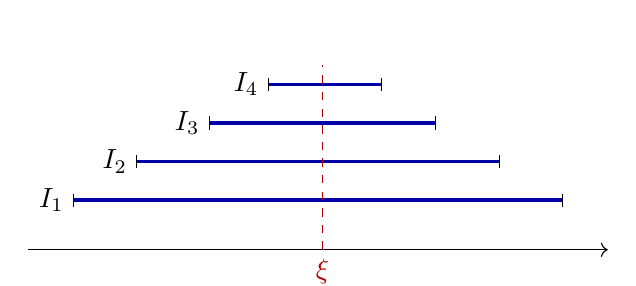
\begin{tikzpicture}[x=1.15cm,y=0.7cm]
  \draw[->] (-0.2,0) -- (6.2,0);
  \foreach \y/\a/\b/\lab in {0.9/0.3/5.7/I_1,1.6/1.0/5.0/I_2,2.3/1.8/4.3/I_3,3.0/2.45/3.7/I_4}
  {
    \draw[very thick,blue!65!black] (\a,\y)--(\b,\y);
    \draw (\a,\y+0.12)--(\a,\y-0.12);
    \draw (\b,\y+0.12)--(\b,\y-0.12);
    \node[left] at (\a,\y) {$\lab$};
  }
  \draw[dashed,red!70!black] (3.05,0)--(3.05,3.35);
  \node[below,red!70!black] at (3.05,0) {$\xi$};
\end{tikzpicture}
\end{center}
\end{intuition}

下面的证明反复把一个有界区间二等分，并选择含有数列无穷多项的半区间。闭区间套性质保证这些不断缩小的闭区间最终确定一个实数点，这个点将成为所构造子列的极限。

\begin{theorem}[博尔查诺--魏尔斯特拉斯（Bolzano--Weierstrass）定理]
\textbf{（有界数列必有收敛子列）}
任何有界数列 \(\{a_n\}\) 必定存在一个收敛的子列 \(\{a_{n_k}\}\)。
\end{theorem}

\begin{custom}{证明}
设 $\{a_n\}$ 有界，则存在闭区间 $I_0=[\alpha_0,\beta_0]$ 包含数列的全部项。 将 $I_0$ 等分为左右两个闭区间。 至少有一个半区间包含数列中的无穷多项；否则两个半区间都只含有限多项，合起来也只含有限多项，与原数列有无穷多项矛盾。 取其中一个含无穷多项的半区间记为 $I_1$。

继续这个过程：把 $I_{k-1}$ 等分，取一个包含数列中无穷多项的半区间 $I_k$。 得到一列闭区间
\[
I_0\supset I_1\supset I_2\supset\cdots,\qquad |I_k|=\frac{|I_0|}{2^k}.
\]
根据闭区间套性质，存在唯一实数 $\xi$ 属于所有 $I_k$，并且区间长度趋于 $0$。

下面从数列中选子列。 因 $I_1$ 含无穷多项，可取 $n_1$ 使 $a_{n_1}\in I_1$。 取定 $n_1,\ldots,n_{k-1}$ 后，由于 $I_k$ 含无穷多项，可选 $n_k>n_{k-1}$ 使 $a_{n_k}\in I_k$。 于是得到子列 $\{a_{n_k}\}$。

任取 $\varepsilon>0$。 因 $|I_k|\to0$，存在 $K$，当 $k\ge K$ 时 $|I_k|<\varepsilon$。 对 $k\ge K$，$a_{n_k}$ 与 $\xi$ 同属 $I_k$，故
\[
|a_{n_k}-\xi|\le |I_k|<\varepsilon.
\]
由极限定义，$a_{n_k}\to\xi$。 因此有界数列必有收敛子列。
\end{custom}

\begin{intuition}

这个定理说的是：如果你有一列数，它们都挤在某个有限的区间里（比如都在 \([-M, M]\) 之间），那么无论它们看起来多么杂乱无章，你总能从中挑出一个“收敛”的子序列。

\textbf{一个生活中的比喻：}

想象一个无限大的体育馆里有无穷多个人，每个人手里拿着一个数字，所有数字都在 0 到 1 之间。你想找出一群人，他们手里的数字越来越接近某个固定值。

博尔查诺--魏尔斯特拉斯定理保证：你一定能找到这样一群人！无论这些人怎么站队，你总能挑出一个子序列，它最终会稳定在某个数附近。

\textbf{一个更直观的几何解释：}

把数列 \(\{a_n\}\) 想象成数轴上的无限个点，所有点都被关在区间 \([-M, M]\) 这个“笼子”里。

\begin{center}
\begin{tikzpicture}[scale=0.8]
\draw[thick, -{Stealth}] (-5,0) -- (5,0) node[right] {数轴};
\draw[thick] (-4,0.1) -- (-4,-0.1) node[below] {\(-M\)};
\draw[thick] (4,0.1) -- (4,-0.1) node[below] {\(M\)};
\draw[thick, red] (-4,0.2) -- (4,0.2) node[above] {笼子（有界区间）};

\foreach \x in {-3.2, -1.5, -0.8, 0.3, 1.2, 2.5, 3.7, -2.1, 0.9, 2.8, -0.2, 1.9, -2.9, 3.1} {
    \filldraw[blue] (\x,0) circle (2pt);
}
\end{tikzpicture}
\end{center}

\textbf{核心思想——二分法：}

你可以用“不断对半分割区间”的方法来构造这个收敛子列：

\begin{enumerate}
\item 一开始，所有点都在区间 \([a, b] = [-M, M]\) 里。
\item 把这个区间分成两半：左边 \([-M, 0]\) 和右边 \([0, M]\)。由于有无穷多个点，至少有一半包含无穷多个点。选择那一半作为新区间 \([a_1, b_1]\)。
\item 再把新区间对半分，同样，至少有一半包含无穷多个点。选择那一半作为 \([a_2, b_2]\)。
\item 如此无限继续下去，我们得到一列不断缩小的区间：
\[
[a, b] \supset [a_1, b_1] \supset [a_2, b_2] \supset \cdots
\]
\item 每次区间的长度减半：\(b_n - a_n = \dfrac{2M}{2^n} \to 0\)。
\item 从每个区间里选出一个数列中的点 \(a_{n_k}\)，这些点就构成了一个收敛的子列。这些点被“挤压”在越来越小的区间里，最终会收敛到区间的公共极限点 \(c\)。
\end{enumerate}

\textbf{一个具体的例子：}

考虑数列 \(a_n = \sin n\)。虽然 \(\sin n\) 在 \([-1, 1]\) 之间振荡，看起来毫无规律，但博尔查诺--魏尔斯特拉斯定理告诉我们：一定存在一个子列收敛。事实上，可以证明 \(\sin n\) 的子列可以收敛到 \([-1, 1]\) 中的任意值，但这个定理只保证“存在”，不告诉我们具体是哪个。

\end{intuition}

\begin{custom}{单调有界准则与博尔查诺--魏尔斯特拉斯定理}

这两个定理是实数完备性的不同表现形式，它们实际上是等价的（在实数系中可以互相推导）。

\begin{tabular}{|c|c|c|}
\hline
 & \textbf{单调有界准则} & \textbf{博尔查诺--魏尔斯特拉斯定理} \\
\hline
\textbf{条件} & 数列单调 + 有界 & 数列有界（不要求单调） \\
\hline
\textbf{结论} & 数列本身收敛 & 存在收敛子列 \\
\hline
\textbf{适用场景} & 单调数列 & 任意有界数列 \\
\hline
\textbf{直观比喻} & 向右走，前面有墙 & 笼子里的无限多只鸟 \\
\hline
\end{tabular}

\textbf{关系：}
\begin{itemize}
\item 在额外具有单调性的条件下，单调有界准则能够推出整个数列收敛，结论更具体。
\item 博尔查诺--魏尔斯特拉斯定理适用于任意有界数列，但只保证其中存在收敛子列。
\item 两个定理的条件和结论不同，不能脱离前提简单地说谁“更强”。它们都是实数完备性的表现形式。
\end{itemize}

\end{custom}
\fi


\iffalse
\subsection*{拓展阅读：Landau 符号-小o与大O}

在分析无穷小量（或无穷大量）时，我们常常需要比较它们趋近于零（或无穷）的“速度”或“阶”。Landau 符号（小 \(o\) 和大 \(O\)）提供了一套简洁的语言来描述这种比较关系。

\textbf{小o记号：高阶无穷小}

\begin{definition}[小o记号]
设 \(b_n\neq0\) 对充分大的 \(n\) 成立。若
\[
\lim_{n\to\infty}\dfrac{a_n}{b_n}=0,
\]
则记作
\[
a_n = o(b_n) \quad (n \to \infty).
\]
当 \(a_n,b_n\to0\) 时，称 \(a_n\) 是比 \(b_n\) 高阶的无穷小；当两者的绝对值趋于无穷时，则表示 \(a_n\) 相对 \(b_n\) 增长更慢。
\end{definition}

\begin{intuition}
\(a_n = o(b_n)\) 的意思是：\(a_n\) 比 \(b_n\) “小得多”，或者说 \(a_n\) 趋近于 0 的速度比 \(b_n\) 快得多。

例如：
\[
\dfrac{1}{n^2} = o\left(\dfrac{1}{n}\right) \quad (n \to \infty),
\]
因为 \(\dfrac{1/n^2}{1/n} = \dfrac{1}{n} \to 0\)。这表示 \(1/n^2\) 比 \(1/n\) 更快地趋于 0。

更常见的用法是 \(a_n = o(1)\)，这直接表示 \(a_n \to 0\)（因为 \(\dfrac{a_n}{1} \to 0\)）。
\end{intuition}

\begin{example}[小o记号的例子]
当 \(n \to \infty\) 时：
\begin{itemize}
\item \(\dfrac{1}{n^2} = o\left(\dfrac{1}{n}\right)\)
\item \(\dfrac{1}{n} = o(1)\)
\item \(\dfrac{\ln n}{n} = o(1)\)
\item \(n = o(n^2)\)
\end{itemize}

\begin{custom}{函数情形的预告}
函数在 \(x\to x_0\) 时的小 \(o\) 记号必须建立在函数极限定义之上，下一章将正式讨论。届时可用
\[
f(x)=g(x)+o\bigl(h(x)\bigr)
\]
表示 \(f(x)-g(x)\) 相对于 \(h(x)\) 是高阶无穷小。
\end{custom}
\end{example}

\textbf{大O记号：同阶或更低阶}

\begin{definition}[大O记号]
设当 \(n\to\infty\) 时，存在常数 \(C>0\) 和正整数 \(N\)，使得当 \(n>N\) 时，
\[
|a_n| \leq C |b_n|,
\]
则称 \(a_n\) 的量级不超过 \(b_n\)，记作
\[
a_n = O(b_n) \quad (n \to \infty).
\]

特别地，若 \(a_n=O(1)\)，表示 \(\{a_n\}\) 是有界数列。函数情形将在正式建立函数极限之后给出。
\end{definition}

\begin{intuition}
\(a_n = O(b_n)\) 的意思是：\(|a_n|\) 不超过 \(|b_n|\) 的某个常数倍。它描述的是“增长（或衰减）速度不超过”的关系。

与 \(o\) 的区别：
\begin{itemize}
\item \(a_n = o(b_n)\) 意味着 \(a_n\) 比 \(b_n\) \textbf{严格更快}地趋于 0（或更慢地趋于无穷），比值趋于 0。
\item \(a_n = O(b_n)\) 意味着 \(a_n\) 与 \(b_n\) 同阶或更低阶，比值有界但不一定趋于 0。
\end{itemize}
\end{intuition}

\begin{example}[大O记号的例子]
当 \(n \to \infty\) 时：
\begin{itemize}
\item \(3n^2 + 2n + 1 = O(n^2)\)（因为 \(\dfrac{3n^2+2n+1}{n^2} \to 3\)，有界）
\item \(n \sin n = O(n)\)（因为 \(|\sin n| \leq 1\)，所以 \(|n \sin n| \leq n\)）
\item \(\dfrac{1}{n} = O\left(\dfrac{1}{n^2}\right)\)？不对！因为 \(\dfrac{1/n}{1/n^2} = n \to \infty\)，无界，所以 \(\dfrac{1}{n}\) 不是 \(O(1/n^2)\)。实际上 \(1/n^2 = O(1/n)\) 才对。
\end{itemize}

\begin{custom}{记号说明}
\(o(b_n)\) 与 \(O(b_n)\) 都不是某个固定数列，而是满足相应渐近条件的一类数列。同一个公式中重复出现的 \(o(b_n)\) 或 \(O(b_n)\)，也不一定代表同一个具体余项。
\end{custom}
\end{example}

\textbf{小o与大O的关系与区别}

\begin{custom}{对比表格}
\begin{tabular}{|c|c|c|}
\hline
\textbf{记号} & \textbf{含义} & \textbf{极限表述} \\
\hline
\(a_n = o(b_n)\) & \(a_n\) 比 \(b_n\) 高阶（或低阶） & \(\lim\limits_{n \to \infty} \dfrac{a_n}{b_n} = 0\) \\
\hline
\(a_n = O(b_n)\) & \(|a_n|\) 不超过 \(|b_n|\) 的常数倍 & \(\left|\dfrac{a_n}{b_n}\right|\) 最终有界 \\
\hline
\(a_n \sim b_n\) & 渐近等价（若二者趋于零，也称等价无穷小） & \(\lim \dfrac{a_n}{b_n} = 1\) \\
\hline
\end{tabular}

\textbf{关系：}
\[
a_n=o(b_n)\quad\Longrightarrow\quad a_n=O(b_n).
\]
反过来一般不成立。例如，\(\sin n=O(1)\) 但 \(\sin n\neq o(1)\)，因为 \(\sin n\) 不趋于 \(0\)。

\textbf{包含关系图：}
\begin{center}
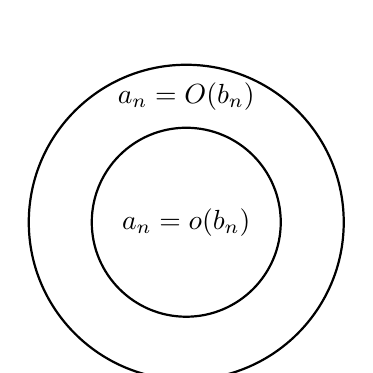
\begin{tikzpicture}
\draw[thick] (0,0) circle (2);
\draw[thick] (0,0) circle (1.2);
\node at (0,0) {$a_n = o(b_n)$};
\node at (0,1.6) {$a_n = O(b_n)$};
\end{tikzpicture}
\end{center}
\end{custom}

\begin{custom}{无穷小与无穷大的关系}
若 \(\{a_n\}\) 是非零无穷小量，则 \(\left\{\dfrac{1}{a_n}\right\}\) 是无穷大量；反之亦然。
\end{custom}

\begin{example}[常见无穷小量的比较]
当 \(n \to \infty\) 时：
\begin{itemize}
\item \(\dfrac{1}{n^p}\)（\(p>0\)）：\(p\) 越大，趋近 0 越快。
\item \(q^n\)（\(0 < q < 1\)）：指数衰减，比任何多项式都快。
\item \(\dfrac{1}{\ln n}\)：衰减极慢。
\item \(\dfrac{1}{n!}\)：衰减极快。
\end{itemize}

\textbf{增长率比较：} 当 \(n \to \infty\) 时，
\[
\ln n \ \ll\ n^p \ \ll\ a^n \ \ll\ n! \ \ll\ n^n \qquad (p>0,\ a>1).
\]
即：对数函数 < 幂函数 < 指数函数 < 阶乘 < \(n^n\)。
\end{example}

\begin{application}[工程：温度传感器的迭代校准]
设 $T_n$ 为第 $n$ 次校准得到的温度估计，标准温度为 $T_{\mathrm s}$，单位均为 $^\circ\mathrm C$。假设每次校准保留上一估计误差的固定比例 $\alpha$，其中 $0<\alpha<1$：
\[
T_{n+1}=\alpha T_n+(1-\alpha)T_{\mathrm s}.
\]
于是
\[
T_{n+1}-T_{\mathrm s}=\alpha(T_n-T_{\mathrm s}),
\qquad
T_n-T_{\mathrm s}=\alpha^{n-1}(T_1-T_{\mathrm s}).
\]
由于 $\alpha^{n-1}\to0$，故 $T_n\to T_{\mathrm s}$。数列极限在这里描述“反复修正最终是否稳定”。模型假设校准比例固定，并忽略随机测量噪声与标准源漂移。
\end{application}

\begin{remark}
农业中的谷物烘干也可出现相同的稳定结构。若第 $n$ 次观测的含水率满足
\[
M_n=M_{\mathrm e}+(M_0-M_{\mathrm e})q^n,\qquad0<q<1,
\]
则 $M_n\to M_{\mathrm e}$，其中 $M_{\mathrm e}$ 是给定环境下的平衡含水率。实际干燥速率会受温度、湿度、气流和谷层厚度影响，这里只作极限直观提示。
\end{remark}
\fi


\begin{extra}
\subsection*{柯西收敛准则（选读）}

\begin{definition}[柯西列]
若对任意 \(\varepsilon > 0\)，存在 \(N\)，当 \(m,n > N\) 时 \(|a_m - a_n| < \varepsilon\)，则称 \(\{a_n\}\) 为柯西列。
\end{definition}
在实数集中，柯西列必收敛（这等价于实数的完备性）。柯西准则的好处是：判断收敛性时不需要知道极限值。
\end{extra}


\iffalse


\subsection*{第2章课后习题}
\addcontentsline{toc}{subsection}{第2章课后习题}

\subsubsection*{第2.1--2.5节\quad 数列的基本概念、表示与差分}

\begin{exercise}写出下列数列的通项公式 \(a_n\)（用 \(n\) 表示）：
\begin{enumerate}
\item \(1, 3, 5, 7, 9, \dots\)
\item \(2, 4, 8, 16, 32, \dots\)
\item \(\dfrac{1}{2}, \dfrac{2}{3}, \dfrac{3}{4}, \dfrac{4}{5}, \dfrac{5}{6}, \dots\)
\item \(1, -\dfrac{1}{2}, \dfrac{1}{3}, -\dfrac{1}{4}, \dfrac{1}{5}, \dots\)
\end{enumerate}
\end{exercise}

\begin{exercise}已知下列递推关系及初始条件，写出数列的前 5 项：
\begin{enumerate}
\item \(a_1 = 3\)，\(a_n = 2a_{n-1}\)（\(n \geq 2\)）
\item \(a_1 = 1\)，\(a_n = a_{n-1} + n\)（\(n \geq 2\)）
\item \(a_1 = 1\)，\(a_2 = 3\)，\(a_n = a_{n-1} - a_{n-2}\)（\(n \geq 3\)）
\end{enumerate}
\end{exercise}

\begin{exercise}对于数列 \(a_n = n^2\)，计算：
\begin{enumerate}
\item 一阶差分 \(\Delta a_n\)
\item 二阶差分 \(\Delta^2 a_n\)
\item 三阶差分 \(\Delta^3 a_n\)
\end{enumerate}
观察结果，你能发现什么规律？
\end{exercise}

\begin{exercise}求下列递推数列的通项公式：
\begin{enumerate}
\item \(a_1 = 1\)，\(a_n = a_{n-1} + 3\)（\(n \geq 2\)）
\item \(a_1 = 5\)，\(a_n = a_{n-1} + 2n - 1\)（\(n \geq 2\)）
\item \(a_1 = 2\)，\(a_n = 2a_{n-1} + 1\)（\(n \geq 2\)）\quad（提示：可设 \(b_n = a_n + 1\) 构造等比数列）
\end{enumerate}
\end{exercise}

\begin{exercise}求一个数列 \(b_n\)，使得 \(\Delta b_n = n \cdot 2^n\)。
提示：设 \(b_n = (An + B)2^n\)，代入确定系数 \(A, B\)。
\end{exercise}

\begin{exercise}用差分法求下列和式：
\begin{enumerate}
\item \(\sum_{k=1}^{n} k\)
\item \(\sum_{k=1}^{n} k(k+1)\)
\end{enumerate}
\end{exercise}

\begin{exercise}已知斐波那契数列：\(F_1 = 1, F_2 = 1, F_n = F_{n-1} + F_{n-2} (n \geq 3)\)。
\begin{enumerate}
\item 计算比值 \(\dfrac{F_6}{F_5}, \dfrac{F_7}{F_6}, \dfrac{F_8}{F_7}, \dfrac{F_9}{F_8}, \dfrac{F_{10}}{F_9}\)，观察它们趋近于哪个数。
\item 证明：\(F_{n+1}F_{n-1} - F_n^2 = (-1)^n\)（卡西尼恒等式）。（选做）
\end{enumerate}
\end{exercise}

\begin{exercise}已知数列 \(\{a_n\}\) 满足 \(a_1 = 1\)，且对任意 \(n \geq 1\) 有 \(\Delta a_n = 3^n\)。
\begin{enumerate}
\item 求 \(a_n\) 的通项公式。
\item 计算 \(\sum_{k=1}^{n} k \cdot 3^{k-1}\)。（提示：利用 \(a_n\) 的表达式）
\end{enumerate}
\end{exercise}

\begin{exercise}已知一个数列的前几项为：\(a_1 = 1, a_2 = 5, a_3 = 14, a_4 = 30, a_5 = 55\)。
\begin{enumerate}
\item 计算该数列的一阶、二阶、三阶差分。
\item 根据差分结果判断 \(a_n\) 可能是几次多项式。
\item 求出 \(a_n\) 的通项公式。
\end{enumerate}
\end{exercise}

\begin{exercise}[较难：递推与差分的综合应用]
设数列 \(\{a_n\}\) 满足 \(a_1 = 1\)，且 \(a_{n+1} = 3a_n + 2^n\)（\(n \geq 1\)）。
\begin{enumerate}
\item 令 \(b_n = \dfrac{a_n}{2^n}\)，写出 \(b_n\) 满足的递推关系。
\item 求 \(b_n\) 的通项公式。
\item 求 \(a_n\) 的通项公式。
\item 计算 \(\sum_{k=1}^{n} a_k\)。
\end{enumerate}
\end{exercise}

\subsubsection*{第2.6--2.15节\quad 实数完备性与数列极限}


\begin{exercise}
用 \(\varepsilon\)-\(N\) 语言来说明这些数列的极限。
\begin{enumerate}
\item \(\lim\limits_{n\to\infty} \dfrac{3}{n} = 0\)
\item \(\lim\limits_{n\to\infty} \dfrac{1}{\sqrt{n}} = 0\)
\item \(\lim\limits_{n\to\infty} \dfrac{5n-2}{n+1} = 5\)
\end{enumerate}
\end{exercise}

\begin{exercise}
\begin{enumerate}
\item 如果数列 \(\{a_n\}\) 收敛，它的极限是否唯一？请简要说明理由。
\item 若 \(\lim\limits_{n\to\infty} a_n = 3\)，证明：存在正整数 \(N\)，使得当 \(n > N\) 时，\(a_n > 2\)。
\item 证明：若数列 \(\{a_n\}\) 收敛，则它必有界。（提示：取 \(\varepsilon = 1\)）
\end{enumerate}
\end{exercise}

\begin{exercise}
\begin{enumerate}
\item 判断下列数列是否为无穷小量：
   \[
   a_n = \dfrac{(-1)^n}{n},\quad b_n = \dfrac{n}{n+1},\quad c_n = 0.99^n,\quad d_n = \ln\left(1+\dfrac{1}{n}\right)
   \]
\item 判断下列数列是否为无穷大量：
   \[
   a_n = n^2,\quad b_n = (-1)^n n,\quad c_n = \ln n,\quad d_n = \dfrac{n^2}{n+1}
   \]
\item 若 \(\{a_n\}\) 是无穷小量且 \(a_n \neq 0\)，证明 \(\left\{\dfrac{1}{a_n}\right\}\) 是无穷大量。
\end{enumerate}
\end{exercise}

\begin{exercise}
用 \(\varepsilon\)-\(N\) 定义证明下列极限：
\begin{enumerate}
\item \(\lim\limits_{n\to\infty} \dfrac{\sin n}{n^2 + 1} = 0\)（提示：\(|\sin n| \leq 1\)）
\item \(\lim\limits_{n\to\infty} \dfrac{3n + \cos n}{2n - 1} = \dfrac{3}{2}\)（提示：先分拆，再放缩）
\end{enumerate}
\end{exercise}

\begin{exercise}
用 \(\varepsilon\)-\(N\) 定义证明：
\[
\lim_{n\to\infty} \left(\sqrt{n^2 + n} - n\right) = \dfrac{1}{2}.
\]
（提示：分子有理化后处理）
\end{exercise}

\begin{exercise}
设常数 \(c > 0\)，证明：
\[
\lim\limits_{n \to \infty} \dfrac{n^c}{a^n} = 0 \quad (a > 1).
\]
（提示：当 \(n\) 足够大时，\(a^n\) 增长快于任何幂函数；可用二项式定理或取对数）
\end{exercise}

\begin{exercise}
证明下列数列发散（极限不存在）：
\begin{enumerate}
\item \(a_n = (-1)^n\)
\item \(a_n = \sin\left(\dfrac{n\pi}{2}\right)\)
\item \(a_n = n + (-1)^n n\)（提示：考虑偶子列和奇子列）
\end{enumerate}
\end{exercise}

\begin{exercise}
用 \(\varepsilon\)-\(N\) 定义证明：
\[
\lim_{n\to\infty} \dfrac{n^2 - 2n + 3}{2n^2 + 5} = \dfrac{1}{2}.
\]
要求明确给出 \(N\) 关于 \(\varepsilon\) 的表达式（可分段处理）。
\end{exercise}

\begin{exercise}
用 \(\varepsilon\)-\(N\) 定义证明：
\begin{enumerate}
\item \(\lim\limits_{n\to\infty} \dfrac{\ln n}{n} = 0\)（提示：先证明当 \(n\) 充分大时 \(\ln n<\sqrt n\)，再取 \(N>\varepsilon^{-2}\)）
\item \(\lim\limits_{n\to\infty} \sqrt[n]{n} = 1\)（提示：设 \(\sqrt[n]{n} = 1 + h_n\)，利用二项式定理证明 \(h_n \to 0\)）
\end{enumerate}
\end{exercise}

\begin{exercise}
设 \(a_n = \dfrac{1}{n^2 + 1} + \dfrac{1}{n^2 + 2} + \cdots + \dfrac{1}{n^2 + n}\)。
\begin{enumerate}
\item 证明：\(\dfrac{n}{n^2 + n} \leq a_n \leq \dfrac{n}{n^2 + 1}\)。
\item 利用夹逼准则求 \(\lim\limits_{n\to\infty} a_n\)。
\item 用 \(\varepsilon\)-\(N\) 定义直接证明该极限。（选做）
\end{enumerate}
\end{exercise}

\begin{exercise}[*（柯西收敛准则）]
设数列 \(\{a_n\}\) 满足：对任意 \(n\)，有 \(|a_{n+1} - a_n| \leq \dfrac{1}{2^n}\)。
\begin{enumerate}
\item 证明：对任意 \(m > n\)，有 \(|a_m - a_n| \leq \dfrac{1}{2^{n-1}}\)。（提示：用三角不等式和等比数列求和）
\item 证明：\(\{a_n\}\) 是柯西列，从而收敛。
\item 若已知 \(a_1 = 1\)，能否求出 \(\lim\limits_{n\to\infty} a_n\)？为什么？
\end{enumerate}
\end{exercise}


\subsection*{第2章参考答案与提示}
\addcontentsline{toc}{subsection}{第2章参考答案与提示}

\subsubsection*{第2.1--2.5节\quad 数列的基本概念、表示与差分}

\begin{enumerate}
\item[(1)] (a) \(a_n = 2n-1\)；(b) \(a_n = 2^n\)；(c) \(a_n = \dfrac{n}{n+1}\)；(d) \(a_n = (-1)^{n-1} \dfrac{1}{n}\)。
\item[(2)] (a) \(3, 6, 12, 24, 48\)；(b) \(1, 3, 6, 10, 15\)；(c) \(1, 3, 2, -1, -3\)。
\item[(3)] \(\Delta a_n = 2n+1\)，\(\Delta^2 a_n = 2\)，\(\Delta^3 a_n = 0\)；规律：\(n^2\) 的二阶差分为常数，三阶及更高阶为 0。
\item[(4)] (a) \(a_n = 3n-2\)；(b) \(a_n = n^2 + 4\)；(c) \(a_n = 2^{n+1} - 1\)。
\item[(5)] \(b_n=(n-2)2^n+C\)（\(C\) 为任意常数）。
\item[(6)] (a) \(\dfrac{n(n+1)}{2}\)；(b) \(\dfrac{n(n+1)(n+2)}{3}\)。
\item[(7)] 比值趋近于 \(\dfrac{1+\sqrt{5}}{2} \approx 1.618\)。
\item[(8)] (a) \(a_n = \dfrac{3^n - 1}{2}\)；(b) \(\sum_{k=1}^{n} k \cdot 3^{k-1} = \dfrac{(2n-1)3^n + 1}{4}\)。
\item[(9)] 三阶差分为常数 \(2\)，是三次多项式，\(a_n=\dfrac{n(n+1)(2n+1)}{6}\)。
\item[(10)] (a) \(b_{n+1}=\dfrac{3}{2}b_n+\dfrac{1}{2}\)；(b) \(b_n=\left(\dfrac{3}{2}\right)^n-1\)；(c) \(a_n=3^n-2^n\)；(d) \(\sum_{k=1}^{n} a_k=\dfrac{3^{n+1}-3}{2}-(2^{n+1}-2)\)。
\end{enumerate}

\subsubsection*{第2.6--2.15节\quad 实数完备性与数列极限}


\begin{enumerate}
\item[(1)] 
   (a) \(N = \lceil 3/\varepsilon \rceil\)；(b) \(N = \lceil 1/\varepsilon^2 \rceil\)；(c) \(\left|\dfrac{5n-2}{n+1} - 5\right| = \dfrac{7}{n+1}\)，取 \(N = \lceil 7/\varepsilon \rceil\)。

\item[(2)] 
   (a) 唯一，反证法用 \(\varepsilon = |L_1 - L_2|/2\) 导出矛盾；(b) 取 \(\varepsilon = 1\)，存在 \(N\) 使 \(n > N\) 时 \(|a_n-3|<1\)，故 \(a_n > 2\)；(c) 取 \(\varepsilon=1\)，有界性证明略。

\item[(3)] 
   (a) 无穷小量：\(a_n, c_n, d_n\)（\(b_n \to 1\) 不是）；(b) 无穷大量：\(a_n,b_n,c_n,d_n\)。其中 \(b_n=(-1)^n n\) 满足 \(|b_n|=n\to\infty\)，但 \(b_n\) 本身既不趋于 \(+\infty\)，也不趋于 \(-\infty\)；(c) 由定义直接验证。

\item[(4)] 
   (a) \(\left|\dfrac{\sin n}{n^2+1}\right| \leq \dfrac{1}{n^2}\)，取 \(N = \lceil 1/\sqrt{\varepsilon} \rceil\)；(b)
   \[
   \frac{3n+\cos n}{2n-1}-\frac32
   =\frac{2\cos n+3}{2(2n-1)},
   \]
   再利用 \(|2\cos n+3|\leq5\) 放缩。

\item[(5)] 
   分子有理化：\(\sqrt{n^2+n} - n = \dfrac{n}{\sqrt{n^2+n}+n} = \dfrac{1}{\sqrt{1+1/n}+1}\)，然后放缩证明。

\item[(6)] 
   取整数 \(m>c\)。当 \(n\geq2m\) 时，由二项式定理，
   \[
   a^n=(1+a-1)^n\geq\binom{n}{m}(a-1)^m
   \geq\frac{(n/2)^m}{m!}(a-1)^m.
   \]
   因而 \(0\leq n^c/a^n\leq Cn^{c-m}\to0\)。

\item[(7)] 
   (a) 子列极限不同；(b) 子列 \(0,1,0,-1,\dots\) 不收敛；(c) \(a_n = n(1+(-1)^n)\)，偶数项 \(\to +\infty\)，奇数项为 0。

\item[(8)] 
   \(\left|\dfrac{n^2-2n+3}{2n^2+5} - \dfrac{1}{2}\right| = \dfrac{4n+1}{2(2n^2+5)} < \dfrac{4n+1}{4n^2} < \dfrac{5}{4n}\)（当 \(n \geq 1\)），取 \(N = \lceil 5/(4\varepsilon) \rceil\)。

\item[(9)] 
   (a) 对充分大的 \(n\)，有 \(\ln n\leq\sqrt n\)，故 \(0\leq \ln n/n\leq1/\sqrt n\to0\)；(b) 由 \(\sqrt[n]{n}=1+h_n\)，二项展开得 \(n=(1+h_n)^n\geq\binom{n}{2}h_n^2\)，故 \(h_n^2\leq\dfrac{2}{n-1}\to0\)。

\item[(10)] 
   (a) 左边放缩：每项 \(\geq \dfrac{1}{n^2+n}\)，共 \(n\) 项；右边放缩：每项 \(\leq \dfrac{1}{n^2+1}\)；(b) 夹逼得极限为 0；(c) 直接证明：\(0 \leq a_n \leq \dfrac{1}{n}\)，取 \(N = \lceil 1/\varepsilon \rceil\)。

\item[(11)] 
   (a) \(|a_m - a_n| \leq \sum_{k=n}^{m-1} |a_{k+1}-a_k| \leq \sum_{k=n}^{\infty} \dfrac{1}{2^k} = \dfrac{1}{2^{n-1}}\)；(b) 由 (a) 知 \(\{a_n\}\) 是柯西列，故收敛；(c) 不能，因为只知道差值大小，不知道具体值。
\end{enumerate}
\fi

\clearpage
\section{无穷级数}

\subsection*{级数概念的引入}

\begin{custom}{芝诺悖论}
古希腊哲学家芝诺说：阿喀琉斯永远追不上乌龟。因为阿喀琉斯每次到达乌龟之前的位置时，乌龟又向前爬了一小段。设阿喀琉斯的速度是乌龟的 10 倍，初始距离为 1。他追到乌龟原位置时，乌龟又爬了 \(0.1\)；他再追 \(0.1\)，乌龟又爬了 \(0.01\)；如此继续，他需要跑的无限段距离是：
\[
1 + 0.1 + 0.01 + 0.001 + \cdots = 1.111\ldots
\]
芝诺认为无限段长度的和是无穷大——但这是错的！

事实上，\(1 + 0.1 + 0.01 + 0.001 + \cdots = \dfrac{10}{9}\) 是有限的。阿喀琉斯只需跑 \(\dfrac{10}{9}\) 的距离就能追上乌龟。
\end{custom}

上述悖论将追赶的总距离分解为无穷多个正数之和。按照有限项求和的经验，人们容易误认为无穷多个正数相加，其结果必然是无穷大，这也是芝诺论证看似成立的根源。然而，有限项加法所满足的运算性质不能随意移植到无穷项的情形。为了准确研究无穷多个数量依次相加是否能够得到一个有限确定的值，我们需要建立 “无穷项求和” 的严格定义，由此引出级数的概念。




\subsection{级数的基本概念}




\begin{definition}[常数项级数]
给定数列 \(\{a_n\}\)，称
\[
\sum_{n=1}^{\infty} a_n = a_1 + a_2 + a_3 + \cdots
\]
为无穷级数，简称级数，\(a_n\) 称为通项。
\end{definition}

\begin{definition}[部分和]
级数 \(\sum\limits_{n = 1}^{  \infty }  a_n\) 的前 \(n\) 项和
\[
S_n = a_1 + a_2 + \cdots + a_n
\]
称为部分和。
\end{definition}

\begin{definition}[级数收敛与发散]
若部分和数列 \(\{S_n\}\) 收敛于 \(S\)，则称级数 \(\sum\limits_{n = 1}^{  \infty } a_n\) 收敛，且和为 \(S\)，记作 \(\sum\limits_{n = 1}^{  \infty } a_n = S\)；若 \(\{S_n\}\) 发散，则称级数发散。
\end{definition}

\begin{custom}{注：}
级数不是“把无穷多个数一次性相加”，而是先形成部分和数列
\[
S_1=a_1,\quad S_2=a_1+a_2,\quad \ldots,\quad S_n=a_1+\cdots+a_n,
\]
再研究 $\{S_n\}$ 是否有极限。 因此级数的敛散性完全由部分和数列决定。
\end{custom}

\begin{example}
判断级数
\[
\sum_{n=1}^{\infty}\frac{1}{n(n+1)}
\]
是否收敛，并求其和。
\end{example}
\begin{solution}
先裂项：
\[
\frac{1}{n(n+1)}=\frac1n-\frac{1}{n+1}.
\]
第 $N$ 个部分和为
\[
S_N=\sum_{n=1}^{N}\left(\frac1n-\frac{1}{n+1}\right)
=1-\frac{1}{N+1}.
\]
由于 $S_N\to1$，故原级数收敛，且
\[
\sum_{n=1}^{\infty}\frac{1}{n(n+1)}=1.
\]
\end{solution}

\subsection*{几何级数}

\begin{example}[几何级数]
几何级数 \(\sum\limits_{n = 1}^{  \infty } ar^n\)（\(a \neq 0\)）：
\[
\sum_{n=0}^{\infty} ar^n = 
\begin{cases}
\dfrac{a}{1-r}, & |r| < 1,\\[6pt]
\text{发散}, & |r| \geq 1.
\end{cases}
\]
\end{example}

\begin{custom}{证明}
当 \(r \neq 1\) 时，部分和为
\[
S_n = a + ar + ar^2 + \cdots + ar^{n-1} = a\dfrac{1-r^n}{1-r}.
\]
\begin{itemize}
\item 若 \(|r| < 1\)，则 \(r^n \to 0\)，所以 \(S_n \to \dfrac{a}{1-r}\)。
\item 若 \(|r| > 1\)，则 \(|r^n| \to \infty\)，\(S_n\) 发散。
\item 若 \(r=1\)，则 \(S_n=na\)，当 \(a\neq0\) 时有 \(|S_n|\to\infty\)。
\item 若 \(r = -1\)，则 \(S_n = a, 0, a, 0, \dots\)，发散。
\end{itemize}
\end{custom}

\begin{example}[应用：循环小数化分数]
将 \(0.333\ldots\) 化为分数。
\end{example}
\begin{solution}
\[
0.333\ldots = \dfrac{3}{10} + \dfrac{3}{100} + \dfrac{3}{1000} + \cdots = \dfrac{3/10}{1-1/10} = \dfrac{3/10}{9/10} = \dfrac{1}{3}.
\]
\end{solution}

\subsection{级数的基本性质}


\begin{property}
	设 $A$ 为非零常数，则级数 $\sum\limits_{n = 1}^{  \infty } A u_n$ 与级数 $\sum\limits_{n = 1}^{  \infty } u_n$ 同时收敛或同时发散。
\end{property}

\begin{custom}{证明}

设级数 $\sum\limits_{n = 1}^{  \infty } A u_n$ 与 $\sum\limits_{n = 1}^{  \infty } u_n$ 的部分和分别记为 $S_n^{\prime}$ 与 $S_n^{\prime \prime}$ ，则有

$$
\begin{aligned}
	S_n^{\prime} & =A u_1+A u_2+\cdots+A u_n \\
	& =A\left(u_1+u_2+\cdots+u_n\right)=A S_n^{\prime \prime}
\end{aligned}
$$

于是，由数列极限的性质可知，极限 $\lim \limits_{n \to \infty} S_n^{\prime}$ 与 $\lim \limits_{n \to \infty} S_n^{\prime \prime}$ 同时存在或同时不存在，即级数 $\sum\limits_{n = 1}^{  \infty } A u_n$ 与 $\sum\limits_{n = 1}^{  \infty } u_n$ 同时收敛或同时发散．且当二极限同时存在时，有 $\lim \limits_{n \to \infty} S_n^{\prime}=$ $A \lim \limits_{n \to \infty} S_n^{\prime \prime}$ ，即有

$$
\sum_{n=1}^{\infty} A u_n=A \sum_{n=1}^{\infty} u_n .
$$

\end{custom}

\begin{property}[级数的线性性质]
	
	
	
若级数 \(\sum\limits_{n = 1}^{  \infty } a_n\) 收敛于 \(S\)，\(\sum\limits_{n = 1}^{  \infty } b_n\) 收敛于 \(T\)，\(\alpha, \beta\) 为常数，则
\[
\sum_{n=1}^{\infty} (\alpha a_n + \beta b_n) = \alpha S + \beta T.
\]
\end{property}

\begin{custom}{证明}
记
\[
A_n=\sum_{k=1}^{n}a_k,\qquad B_n=\sum_{k=1}^{n}b_k.
\]
由条件 $A_n\to S,\ B_n\to T$。 对级数 $\sum(\alpha a_n+\beta b_n)$，其第 $n$ 个部分和为
\[
\sum_{k=1}^{n}(\alpha a_k+\beta b_k)=\alpha A_n+\beta B_n.
\]
由收敛数列四则运算法则，
\[
\alpha A_n+\beta B_n\to \alpha S+\beta T.
\]
因此该级数收敛，且和为 $\alpha S+\beta T$。
\end{custom}

\begin{property}[添加或删除有限项]
在级数中添加、删除或改变有限项，不改变级数的敛散性。但若级数收敛，其和可能会改变。
\end{property}

\begin{custom}{证明}
以改变前 $m$ 项为例。 设原级数部分和为
\[
S_n=a_1+\cdots+a_n,
\]
改变前 $m$ 项后得到的新级数部分和记为 $T_n$。 当 $n>m$ 时，$T_n$ 与 $S_n$ 只相差一个固定常数 $C$，即
\[
T_n=S_n+C.
\]
若 $S_n$ 收敛，则 $T_n$ 也收敛；若 $S_n$ 发散而 $T_n$ 收敛，则 $S_n=T_n-C$ 收敛，矛盾。 因此二者敛散性相同。 当收敛时，极限值相差 $C$，所以级数和可能改变。
\end{custom}

\begin{property}[加括号]
收敛级数任意加括号后所成的新级数仍然收敛，且和不变。

\textbf{注意：} 逆命题不成立。即加括号后收敛的级数，原级数未必收敛。例如：
\[
(1-1)+(1-1)+(1-1)+\cdots = 0+0+0+\cdots = 0,
\]
但原级数 \(1-1+1-1+1-1+\cdots\) 是发散的。
\end{property}

\begin{custom}{证明}
设原级数 $\sum\limits_{n = 1}^{  \infty } a_n$ 的部分和 $S_n\to S$。 任意加括号后，新级数的部分和等于原部分和数列中的一个子列：
\[
T_k=S_{n_k},\qquad 1\le n_1<n_2<\cdots .
\]
收敛数列的任意子列收敛到同一极限，因此 $T_k\to S$。 所以加括号后的级数仍收敛，且和不变。 逆命题不成立的例子如定理中所示。
\end{custom}



\begin{property}[级数收敛的必要条件]
若 \(\sum\limits_{n = 1}^{  \infty } a_n\) 收敛，则 \(\lim\limits_{n \to \infty} a_n = 0\)。
\end{property}

\begin{custom}{证明}
设部分和 \(S_n \to S\)，则 \(a_n = S_n - S_{n-1} \to S - S = 0\)。\(\square\)
\end{custom}

\textbf{注意：} 这个条件是必要的，但不是充分的。也就是说，\(a_n \to 0\) 不能保证级数收敛。

\begin{example}[调和级数]
调和级数 \(\sum\limits_{n = 1}^{  \infty } \dfrac{1}{n}\) 虽然通项 \(\dfrac{1}{n} \to 0\)，但它是发散的。
\end{example}
\begin{custom}{证明}
考虑部分和 \(S_{2^n}\)：
\[
S_{2^n} = 1 + \dfrac12 + \left(\dfrac13+\dfrac14\right) + \left(\dfrac15+\cdots+\dfrac18\right) + \cdots + \left(\dfrac{1}{2^{n-1}+1} + \cdots + \dfrac{1}{2^n}\right).
\]
$\dfrac13+\dfrac14 > \dfrac14 \times 2 =\dfrac12$,$\dfrac15+\cdots+\dfrac18>\dfrac18 \times 4 =\dfrac12$,以此类推，第 \(k\) 组有 \(2^{k-1}\) 项，每项不小于 \(1/2^k\)，每一括号的和至少为 \(\dfrac12\)，所以
\[
S_{2^n}\geq1+\dfrac n2\to\infty.
\]
故调和级数发散。
\end{custom}

\subsection{正项级数及其判别法}

\begin{theorem}
	设 $\sum\limits_{n = 1}^{  \infty } a_n$ 为正项级数，则 $\sum\limits_{n = 1}^{  \infty }a_n$ 收敛的充分必要条件是它的部分和数列有上界．
\end{theorem}


\begin{custom}{证明}
由 $a_n \geqslant 0(n=1,2, \cdots)$ 可知

$$
S_{n+1}=S_n+a_{n+1} \geqslant S_n \geqslant 0, \quad n \in N .
$$

可见 $\left\{S_n\right\}$ 是单调增加数列．因此，由定理 2.7 可知，若 $\left\{S_n\right\}$ 有上界，则极限 $\lim \limits_{n \to \infty} S_n$存在，从而 $\sum\limits_{n = 1}^{  \infty } a_n$ 收敛，充分性得证；若 $\left\{S_n\right\}$ 无上界，则 $\lim \limits_{n \to \infty} S_n=+\infty$ ，从而 $\sum\limits_{n = 1}^{  \infty } a_n$ 发散，换句话说，若数列收敛，则部分和数列 $\left\{S_n\right\}$ 必有上界，必要性得证．定理得证．

\end{custom}

\begin{theorem}[比较判别法]
设 \(\sum\limits_{n = 1}^{  \infty } a_n\) 和 \(\sum\limits_{n = 1}^{  \infty } b_n\) 为正项级数，且存在 \(N\)，当 \(n > N\) 时 \(a_n \leq b_n\)。
\begin{enumerate}
\item 若 \(\sum\limits_{n = 1}^{  \infty } b_n\) 收敛，则 \(\sum\limits_{n = 1}^{  \infty } a_n\) 收敛；
\item 若 \(\sum\limits_{n = 1}^{  \infty } a_n\) 发散，则 \(\sum\limits_{n = 1}^{  \infty } b_n\) 发散。
\end{enumerate}
\end{theorem}

\begin{custom}{证明}
只需考虑从 $N+1$ 项开始的尾级数，因为添加或删除有限项不改变敛散性。 记
\[
A_m=\sum_{n=N+1}^{m}a_n,\qquad B_m=\sum_{n=N+1}^{m}b_n.
\]
由于 $0\le a_n\le b_n$，所以对所有 $m>N$ 有
\[
0\le A_m\le B_m.
\]
若 $\sum\limits_{n = 1}^{  \infty } b_n$ 收敛，则 $\{B_m\}$ 有上界，从而 $\{A_m\}$ 是单调递增且有上界的数列，由单调有界准则知 $\{A_m\}$ 收敛，故 $\sum\limits_{n = 1}^{  \infty } a_n$ 收敛。

第二个结论是第一个结论的逆否命题：若 $\sum\limits_{n = 1}^{  \infty } b_n$ 收敛，则 $\sum\limits_{n = 1}^{  \infty } a_n$ 收敛。 因此若 $\sum\limits_{n = 1}^{  \infty } a_n$ 发散，$\sum\limits_{n = 1}^{  \infty } b_n$ 不可能收敛，只能发散。
\end{custom}

\begin{intuition}
比较判别法的道理很简单：想象你在往一个杯子里倒水。

如果 \(b_n\) 代表“大杯子”倒进去的水量，而 \(\sum\limits_{n = 1}^{  \infty } b_n\) 收敛意味着这个大杯子里的水总量是有限的（不会溢出）。那么，比它更小的 \(a_n\)（小杯子）倒进去的水总量当然更有限——肯定也收敛。

反过来，如果你知道小杯子 \(\sum\limits_{n = 1}^{  \infty } a_n\) 的水量已经无限大（发散），那么比它更大的大杯子 \(\sum\limits_{n = 1}^{  \infty } b_n\) 的水量一定也无限大。

一句话总结：\textbf{大的收敛，小的必收敛；小的发散，大的必发散。}
\end{intuition}


\begin{corollary}
	设 $\sum\limits_{n = 1}^{  \infty } u_n$ 和 $\sum\limits_{n = 1}^{  \infty } v_n$ 为正项级数，且存在常数 $c>0$ 和自然数 $N$ ，使当$n>N$ 时，有
	
	$$
	u_n \leqslant c v_n .
	$$
	
	则有
	\begin{itemize}
		\item[（1）] 当 $\sum\limits_{n = 1}^{  \infty } v_n$ 收敛时，$\sum\limits_{n = 1}^{  \infty } u_n$ 收敛；
		\item[（2）] 当 $\sum\limits_{n = 1}^{  \infty } u_n$ 发散时，$\sum\limits_{n = 1}^{  \infty } v_n$ 发散．
	\end{itemize}
\end{corollary}

\begin{example}
判断级数 \(\sum\limits_{n = 1}^{  \infty } \dfrac{1}{n!}\) 的敛散性。
\end{example}

\begin{solution}
当 \(n \geq 1\) 时，\(n! = 1 \cdot 2 \cdot 3 \cdots n \geq 1 \cdot 2 \cdot 2 \cdots 2 = 2^{n-1}\)，因此
\[
\dfrac{1}{n!} \leq \dfrac{1}{2^{n-1}}.
\]

而几何级数 \(\sum\limits_{n = 1}^{  \infty } \dfrac{1}{2^{n-1}} = 1 + \dfrac12 + \dfrac14 + \cdots = 2\) 是收敛的。由比较判别法，\(\sum\limits_{n = 1}^{  \infty } \dfrac{1}{n!}\) 也收敛。

事实上，这个级数的和就是自然常数 \(\ee\)：
\[
\ee = \sum_{n=0}^{\infty} \dfrac{1}{n!} = 1 + 1 + \dfrac12 + \dfrac16 + \dfrac{1}{24} + \cdots \approx 2.71828.
\]
\end{solution}

\begin{example}
判断 \(\sum\limits_{n = 1}^{  \infty } \dfrac{1}{n^2}\) 的敛散性。
\end{example}
\begin{solution}
当 \(n \geq 2\) 时，\(\dfrac{1}{n^2} \leq \dfrac{1}{n(n-1)} = \dfrac{1}{n-1} - \dfrac{1}{n}\)。
而 \(\sum\limits_{n = 2}^{  \infty } \left(\dfrac{1}{n-1} - \dfrac{1}{n}\right) = 1\) 收敛，故 \(\sum\limits_{n = 1}^{  \infty } \dfrac{1}{n^2}\) 收敛。
\end{solution}

\begin{example}[\(p\)-级数]
\[
\sum_{n=1}^{\infty} \dfrac{1}{n^p}
\]
当 \(p > 1\) 时收敛，当 \(p \leq 1\) 时发散。
\end{example}

\begin{custom}{证明}
先设 $p>1$。 将 $n\ge2$ 的项按
\[
2^k\le n\le 2^{k+1}-1\qquad(k=0,1,2,\ldots)
\]
分组。 在第 $k$ 组中共有 $2^k$ 项，且每项不超过 $1/(2^k)^p$，故该组和不超过
\[
2^k\cdot \frac{1}{(2^k)^p}=2^{k(1-p)}.
\]
因为 $p>1$，几何级数 $\sum\limits_{k = 0}^{  \infty }2^{k(1-p)}$ 收敛，由比较判别法知 $\sum\limits_{n = 1}^{  \infty } 1/n^p$ 收敛。

若 $p=1$，得到调和级数，前文已经证明其发散。 若 $p<1$，则对 $n\ge1$ 有 $n^p\le n$，从而
\[
\frac1{n^p}\ge \frac1n.
\]
由比较判别法，$\sum\limits_{n = 1}^{  \infty } 1/n^p$ 发散。
\end{custom}

\begin{intuition}
\(p=1\) 是调和级数，发散；\(p=2\) 收敛；\(p=0.5\) 的项比调和级数对应项更大，因而其部分和增长得更快。参数 \(p\) 越大，通项衰减越快。
\end{intuition}

\begin{theorem}[比值判别法（达朗贝尔判别法）]
设 \(\sum\limits_{n = 1}^{  \infty }a_n\) 为正项级数，若 \(\lim\limits_{n\to\infty}\dfrac{a_{n+1}}{a_n}=\rho\)，则
\begin{itemize}
\item 若 \(\rho < 1\)，级数收敛；
\item 若 \(\rho > 1\)（包括 \(\rho = +\infty\)），级数发散；
\item 若 \(\rho = 1\)，判别法失效，需用其他方法判断。
\end{itemize}
\end{theorem}

\begin{custom}{证明}
若 $\rho<1$，取常数 $r$ 使 $\rho<r<1$。 由极限定义，存在 $N$，当 $n\ge N$ 时
\[
\frac{a_{n+1}}{a_n}\le r.
\]
于是
\[
a_{N+k}\le a_N r^k\qquad(k=1,2,\ldots).
\]
尾级数 $\sum\limits_{k = 1}^{  \infty }a_N r^k$ 是收敛的几何级数，由比较判别法，$\sum\limits_{n = 1}^{  \infty } a_n$ 收敛。

若 $\rho>1$，取 $r$ 使 $1<r<\rho$。 则存在 $N$，当 $n\ge N$ 时
\[
\frac{a_{n+1}}{a_n}\ge r>1.
\]
因此 $a_{n+1}\ge a_n$ 对充分大的 $n$ 成立，且 $a_n$ 不可能趋于 $0$。 由级数收敛的必要条件，$\sum\limits_{n = 1}^{  \infty } a_n$ 发散。 当 $\rho=+\infty$ 时同理可取任意 $r>1$。

当 $\rho=1$ 时，该方法不能给出结论。 例如 $\sum\limits_{n = 1}^{  \infty } 1/n$ 发散而 $\sum\limits_{n = 1}^{  \infty } 1/n^2$ 收敛，二者的相邻项比值极限都为 $1$。
\end{custom}

\begin{intuition}
比值判别法的道理是：如果相邻两项的比值趋于一个小于 1 的数，那么级数的项最终会像一个公比小于 1 的几何级数那样衰减，从而收敛；如果比值趋于大于 1，则项会越来越大，级数发散。
\end{intuition}

\begin{example}
判断级数 \(\sum\limits_{n = 1}^{  \infty } \dfrac{2^n}{n!}\) 的敛散性。
\end{example}
\begin{solution}
\[
\dfrac{a_{n+1}}{a_n} = \dfrac{2^{n+1}}{(n+1)!} \cdot \dfrac{n!}{2^n} = \dfrac{2}{n+1} \to 0 < 1,
\]
由比值判别法，级数收敛。
\end{solution}

\begin{theorem}[根值判别法（柯西判别法）]
设 \(\sum\limits_{n = 1}^{  \infty } a_n\) 为正项级数，且 \(\lim\limits_{n\to\infty} \sqrt[n]{a_n} = \rho\)，则
\begin{itemize}
\item 若 \(\rho < 1\)，级数收敛；
\item 若 \(\rho > 1\)（包括 \(\rho = +\infty\)），级数发散；
\item 若 \(\rho = 1\)，判别法失效。
\end{itemize}
\end{theorem}

\begin{custom}{证明}
若 $\rho<1$，取 $r$ 使 $\rho<r<1$。 由极限定义，存在 $N$，当 $n\ge N$ 时
\[
\sqrt[n]{a_n}\le r,
\]
即 $a_n\le r^n$。 因 $\sum\limits_{n = 1}^{  \infty } r^n$ 收敛，由比较判别法知 $\sum\limits_{n = 1}^{  \infty } a_n$ 收敛。

若 $\rho>1$，取 $r$ 使 $1<r<\rho$。 则存在 $N$，当 $n\ge N$ 时
\[
\sqrt[n]{a_n}\ge r,
\]
从而 $a_n\ge r^n>1$。 因此 $a_n$ 不趋于 $0$，由级数收敛的必要条件，$\sum\limits_{n = 1}^{  \infty } a_n$ 发散。 $\rho=+\infty$ 的情形同理。

当 $\rho=1$ 时，该判别法不能区分 $\sum\limits_{n = 1}^{  \infty } 1/n$ 与 $\sum\limits_{n = 1}^{  \infty } 1/n^2$ 这类情形，因此失效。
\end{custom}

\begin{example}
判断级数 \(\sum\limits_{n = 1}^{  \infty } \left(\dfrac{n}{2n+1}\right)^n\) 的敛散性。
\end{example}
\begin{solution}
\[
\sqrt[n]{a_n} = \dfrac{n}{2n+1} = \dfrac{1}{2 + \dfrac{1}{n}} \to \dfrac{1}{2} < 1,
\]
由根值判别法，级数收敛。
\end{solution}

\subsection{任意项级数的敛散性及其判别法}

\begin{definition}[绝对收敛]
	若级数 \(\sum\limits_{n = 1}^{  \infty } |a_n|\) 收敛，则称 \(\sum\limits_{n = 1}^{  \infty } a_n\) 绝对收敛。
\end{definition}

\begin{definition}[条件收敛]
	若 \(\sum\limits_{n = 1}^{  \infty } a_n\) 收敛，但 \(\sum\limits_{n = 1}^{  \infty } |a_n|\) 发散，则称 \(\sum\limits_{n = 1}^{  \infty } a_n\) 条件收敛。
\end{definition}

\begin{theorem}[绝对收敛与收敛的关系]
	绝对收敛的级数一定收敛。即若 \(\sum\limits_{n = 1}^{  \infty } |a_n|\) 收敛，则 \(\sum\limits_{n = 1}^{  \infty } a_n\) 必收敛。
\end{theorem}

\begin{custom}{证明}
	定义
	\[
	a_n^+=\frac{|a_n|+a_n}{2},\qquad a_n^-=\frac{|a_n|-a_n}{2}.
	\]
	则 $a_n^+\ge0,\ a_n^-\ge0$，且
	\[
	a_n=a_n^+-a_n^-,\qquad 0\le a_n^+\le |a_n|,\quad 0\le a_n^-\le |a_n|.
	\]
	若 $\sum\limits_{n = 1}^{  \infty } |a_n|$ 收敛，由比较判别法，正项级数 $\sum\limits_{n = 1}^{  \infty } a_n^+$ 与 $\sum\limits_{n = 1}^{  \infty } a_n^-$ 都收敛。 由级数线性性质，
	\[
	\sum_{n=1}^{\infty} a_n=\sum_{n=1}^{\infty} a_n^+-\sum_{n=1}^{\infty} a_n^-
	\]
	收敛。 因此绝对收敛必推出收敛。
\end{custom}

\begin{intuition}
	\begin{itemize}
		\item \textbf{绝对收敛：} 无论你把所有项都取正（去掉符号），总和仍然是有限的。这类级数最“乖”，可以随意重排顺序而不改变和。
		\item \textbf{条件收敛：} 你之所以能得到有限的和，完全是因为正负项互相抵消。如果把所有项都取正，总和就会变成无穷大。这类级数很“敏感”，重排顺序可能会改变和（甚至变成发散）。
	\end{itemize}
\end{intuition}

\begin{example}
	\begin{itemize}
		\item 级数 \(\sum\limits_{n = 1}^{  \infty } \dfrac{(-1)^{n-1}}{n^2}\) 绝对收敛，因为 \(\sum\limits_{n = 1}^{  \infty } \dfrac{1}{n^2}\) 收敛。
		\item 交错调和级数 \(\sum\limits_{n = 1}^{  \infty } \dfrac{(-1)^{n-1}}{n}\) 条件收敛，因为它本身收敛，但 \(\sum\limits_{n = 1}^{  \infty } \dfrac{1}{n}\) 发散。
	\end{itemize}
\end{example}

\begin{remark}
	条件收敛是一个相当微妙的概念。一个著名的定理（黎曼重排定理）说：条件收敛的级数，可以通过重排使其收敛到任意实数，甚至发散！这再次提醒我们，无穷级数中的“加法”与有限和的加法有着本质的不同。
\end{remark}



\begin{definition}[交错级数]
$b_n > 0$,形如
\[
\sum_{n=1}^{\infty} (-1)^{n-1} b_n = b_1 - b_2 + b_3 - b_4 + \cdots \quad 
\]
的级数称为交错级数。
\end{definition}

\begin{theorem}[莱布尼茨判别法]
若交错级数 \(\sum_{n=1}^{\infty} (-1)^{n-1} b_n\) 满足：
\begin{enumerate}
\item \(b_n\) 单调递减,即 \(b_1 \geq b_2 \geq b_3 \geq \cdots\)；
\item \(\lim\limits_{n\to\infty} b_n = 0\)，
\end{enumerate}
则级数收敛，且其和 \(S\) 满足 \(\boxed{0\leq S\leq b_1}\)，余项满足
\[
\boxed{|R_n|\le b_{n+1}}.
\]
\end{theorem}

\begin{custom}{证明}
记部分和为 $S_n=\sum\limits_{k=1}^{n}(-1)^{k-1}b_k$。 偶数项部分和满足
\[
S_{2m+2}-S_{2m}=b_{2m+1}-b_{2m+2}\ge0,
\]
故 $\{S_{2m}\}$ 单调递增。 又
\[
S_{2m}=(b_1-b_2)+\cdots+(b_{2m-1}-b_{2m})\ge0,
\]
且
\[
S_{2m}=b_1-(b_2-b_3)-\cdots-(b_{2m-2}-b_{2m-1})-b_{2m}\le b_1.
\]
因此 $\{S_{2m}\}$ 单调有界，设其极限为 $S$。

奇数项部分和满足
\[
S_{2m+1}=S_{2m}+b_{2m+1}.
\]
因 $b_{2m+1}\to0$，得 $S_{2m+1}\to S$。 偶数子列和奇数子列趋于同一极限，所以 $S_n\to S$，级数收敛。 由 $0\le S_{2m}\le S\le S_{2m+1}\le b_1$ 可得 $0\le S\le b_1$。 若进一步假设 $b_n>0$ 且严格单调递减，则可进一步得到 $0<S<b_1$。

余项估计来自同样的夹逼。 从第 $n+1$ 项起的尾和是首项为 $b_{n+1}$、项的绝对值单调趋零的交错和，其值位于 $0$ 与首项之间或二者相反数之间，所以
\[
|R_n|\le b_{n+1}.
\]
若进一步假设 $b_n>0$ 且严格单调递减，则可进一步得到 $|R_n|<b_{n+1}$；主定理统一采用非严格估计。
\end{custom}

\begin{intuition}
交错级数像一个人在左右摇摆：第一步向右走 \(b_1\)，第二步向左走 \(b_2\)，第三步向右走 \(b_3\)……如果每一步的步长越来越小（单调递减），并且最终步长趋近于零，那么这个人会逐渐稳定在一个点上，而不会无限摇摆下去。
\end{intuition}

\begin{example}
判断交错调和级数 \(\sum\limits_{n=1}^{\infty} (-1)^{n-1} \dfrac{1}{n} = 1 - \dfrac12 + \dfrac13 - \dfrac14 + \cdots\) 的敛散性。
\end{example}
\begin{solution}
这里 \(b_n = \dfrac{1}{n}\) 单调递减趋于 0，满足莱布尼茨判别法的条件，故级数收敛。

值得注意的是：调和级数 \(\sum \limits_{n=1}^{\infty}\dfrac{1}{n}\) 是发散的，但给它加上交错符号后却收敛了。这说明正负交替可以“抵消”掉部分发散性。
\end{solution}


\subsection*{判别法小结}

\begin{tabular}{|c|c|c|}
\hline
\textbf{判别法} & \textbf{适用类型} & \textbf{结论} \\
\hline
比较判别法 & 正项级数 & 需已知一个比较级数 \\
\hline
比值判别法 & 正项级数（含阶乘、指数） & \(\rho < 1\) 收敛，\(\rho > 1\) 发散 \\
\hline
根值判别法 & 正项级数（含 \(n\) 次幂） & \(\rho < 1\) 收敛，\(\rho > 1\) 发散 \\
\hline
莱布尼茨判别法 & 交错级数 & 单调递减趋于 0 则收敛 \\
\hline
\end{tabular}



\begin{application}[几何级数在金融中的运用：永续年金]

假设你有一笔资金存入银行，希望每年年末都能领取固定金额 \(A\) 元，且本金永不减少（即每年只领取利息，本金保持不变）。设年利率为 \(i>0\)，问最初需要存入多少本金？

\textbf{分析：}
\begin{itemize}
\item 要保证每年年末领取 \(A\) 元，第一年末领取的 \(A\) 元来源于本金的利息。
\item 更一般的思路是：将未来每年领取的 \(A\) 元折算到当前，其现值之和应等于最初存入的本金。
\item 第 \(k\) 年末领取的 \(A\) 元，折现到当前的价值为 \(\dfrac{A}{(1+i)^k}\)。
\end{itemize}

因此，最初需要存入的本金为：
\[
P = \frac{A}{1+i} + \frac{A}{(1+i)^2} + \frac{A}{(1+i)^3} + \cdots
\]

这是一个首项 \(a=\dfrac{A}{1+i}\)、公比 \(q=\dfrac{1}{1+i}\) 的几何级数。由于 \(0<q<1\)，级数收敛，其和为：
\[
P=\frac{\frac{A}{1+i}}{1-\frac{1}{1+i}}
=\frac{A}{1+i}\cdot\frac{1+i}{i}
=\frac{A}{i}.
\]

\textbf{结论：} 永续年金的现值公式为 \(P=\dfrac{A}{i}\)。例如，若年利率为 \(5\%\)，希望每年末领取 10000 元，则最初需要存入 \(P=\dfrac{10000}{0.05}=200000\) 元。

\textbf{注：} 这个公式在养老金设计、 endowment fund（捐赠基金）等场景中广泛应用。
\end{application}

\begin{application}[几何级数在医学中的运用：药物浓度累积]

下面使用一个简化的单室、线性叠加模型说明几何级数。假设每次给药带来的浓度增量相同，药物浓度按指数规律衰减：经过时间 \(\Delta t\) 后，单次给药所贡献的浓度降至原来的 \(\ee^{-k\Delta t}\) 倍。

设每次注射后体内药物的初始浓度为 \(C_0\)，每隔时间 \(T\) 注射一次。则：
\begin{itemize}
\item 第一次注射后，体内药物浓度为 \(C_0\)。
\item 第二次注射前，第一次注射的药物浓度已衰减为 \(C_0\ee^{-kT}\)。第二次注射后，模型给出的峰浓度为 \(C_0+C_0\ee^{-kT}\)。
\item 第三次注射前，前两次的药物浓度分别衰减为 \(C_0\ee^{-2kT}\) 和 \(C_0\ee^{-kT}\)。第三次注射后的峰浓度为 \(C_0+C_0\ee^{-kT}+C_0\ee^{-2kT}\)。
\item 依此类推，第 \(n\) 次注射后的模型峰浓度为：
\[
C_n=C_0\left(1+\ee^{-kT}+\ee^{-2kT}+\cdots+\ee^{-(n-1)kT}\right).
\]
\end{itemize}

这是一个首项为 \(C_0\)、公比为 \(\ee^{-kT}\) 的几何级数部分和。由于 \(0<\ee^{-kT}<1\)，当 \(n\to\infty\) 时，给药后峰浓度趋于稳态峰值：
\[
C_{\infty}=\lim_{n\to\infty}C_n=\frac{C_0}{1-\ee^{-kT}}.
\]

\textbf{模型说明：} 该公式只展示重复给药的累积效应，不能直接用于确定临床剂量。实际的负荷剂量与维持剂量还取决于目标浓度、分布容积、清除率、生物利用度和给药间隔等，并需由专业人员结合患者情况确定。\upcite{NCBISteadyState} 例如，若一个给药间隔恰好等于半衰期，即 \(\ee^{-kT}=1/2\)，则本模型中的稳态峰值是单次给药初始峰值的 \(1/(1-0.5)=2\) 倍。

\textbf{一个小计算：} 若模型中每次给药带来的初始浓度增量为 \(10\,\text{mg/L}\)，每 8 小时给药一次，且 \(\ee^{-8k}=0.6\)，则稳态峰值为：
\[
C_{\infty} = \frac{10}{1 - 0.6} = \frac{10}{0.4} = 25\,\text{mg/L}.
\]
\end{application}

\begin{application}[工程：多次反射与信号衰减]
设初始信号能量为 $E_0$，每经过一次反射后保留固定比例 $r$，其中 $0<r<1$。若各级反射分量在接收端按能量相加，则总贡献为
\[
E=E_0+E_0r+E_0r^2+\cdots
=\frac{E_0}{1-r}.
\]
若 $E_0=2\ \mathrm{mJ}$、$r=0.3$，则 $E=20/7\ \mathrm{mJ}$。这一几何级数结构可用于理解声学回声、光学多次反射或通信中的重复衰减分量。模型忽略了相位干涉、频率依赖和随传播路径变化的衰减，因此只用于说明级数累积。
\end{application}

\iffalse


\subsection*{第3章课后习题}
\addcontentsline{toc}{subsection}{第3章课后习题}
\begin{exercise}[级数练习题]
判断下列级数的敛散性：

\begin{enumerate}
\item \(\sum_{n=1}^{\infty} \dfrac{n}{2n+1}\)
\item \(\sum_{n=1}^{\infty} \dfrac{3^{n-1}}{4^n}\)
\item \(\sum_{n=1}^{\infty} \dfrac{2^n}{n^2}\)
\item \(\sum_{n=1}^{\infty} \dfrac{1}{n(n+1)}\)
\item \(\sum_{n=1}^{\infty} \dfrac{n!}{10^n}\)
\item \(\sum_{n=1}^{\infty} (-1)^{n-1} \dfrac{1}{\sqrt{n}}\)
\item \(\sum_{n=1}^{\infty} \dfrac{\sin n}{n^2}\)
\item \(\sum_{n=1}^{\infty} \left(\dfrac{1}{n^p} - \dfrac{1}{(n+1)^p}\right) \quad (p>0)\)
\end{enumerate}
\end{exercise}

\subsection*{第3章参考答案与提示}
\addcontentsline{toc}{subsection}{第3章参考答案与提示}
\begin{enumerate}
\item 发散（通项 \(\to \dfrac12 \neq 0\)）
\item 收敛（公比 \(r = \dfrac34 < 1\) 的几何级数）
\item 发散（通项 \(\to \infty\)）
\item 收敛（裂项相消，部分和 \(S_n = 1 - \dfrac{1}{n+1} \to 1\)）
\item 发散（比值 \(\dfrac{a_{n+1}}{a_n} = \dfrac{n+1}{10} \to \infty > 1\)）
\item 条件收敛（莱布尼茨判别法，但 \(p=1/2 < 1\) 故不绝对收敛）
\item 绝对收敛（\(|\sin n| \leq 1\)，比较 \(\dfrac{1}{n^2}\)）
\item 收敛（裂项相消，\(S_n = \dfrac{1}{1^p} - \dfrac{1}{(n+1)^p} \to 1\)）
\end{enumerate}

\fi

\clearpage
\section{函数极限与连续性}

\subsection{一元函数极限}

数列极限研究的是离散点列 \(a_1,a_2,\ldots\) 的变化趋势；函数极限研究的则是自变量在某个点附近连续变化时，函数值的变化趋势。讨论 \(x\to x_0\) 时，只关心 \(x\) 充分接近 \(x_0\) 且 \(x\neq x_0\) 的情形，这一区域称为 \(x_0\) 的\textbf{去心邻域}。

\begin{definition}[函数极限的\(\varepsilon\)--\(\delta\) 语言]
设函数 \(f\) 在点 \(x_0\) 的某个去心邻域内有定义。若存在常数 \(A\)，使得对任意 \(\varepsilon>0\)，总存在 \(\delta>0\)，当
\[
0<|x-x_0|<\delta
\]
时都有
\[
|f(x)-A|<\varepsilon,
\]
则称当 \(x\to x_0\) 时 \(f(x)\) 的极限为 \(A\)，记作
\[
\lim_{x\to x_0}f(x)=A.
\]
\end{definition}

定义中的逻辑次序是“先给误差要求 \(\varepsilon\)，再寻找自变量范围 \(\delta\)”。\(\delta\) 可以依赖于 \(\varepsilon\)，但不能依赖于邻域中临时选取的 \(x\)。

\begin{example}[按定义证明函数极限]
证明
\[
\lim_{x\to2}(3x-1)=5.
\]
\end{example}
\begin{proofdetail}
任取 \(\varepsilon>0\)。注意到
\[
|(3x-1)-5|=3|x-2|.
\]
取 \(\delta=\varepsilon/3\)，则当 \(0<|x-2|<\delta\) 时，
\[
|(3x-1)-5|<3\delta=\varepsilon.
\]
因此 \(\lim_{x\to2}(3x-1)=5\)。
\end{proofdetail}

\begin{custom}{极限与函数在该点的取值无关}
函数极限只考察去心邻域，所以 \(f(x_0)\) 可以等于极限、不同于极限，甚至没有定义。例如
\[
f(x)=
\begin{cases}
\dfrac{x^2-1}{x-1},&x\neq1,\\
100,&x=1
\end{cases}
\]
满足 \(\lim_{x\to1}f(x)=2\)，尽管 \(f(1)=100\)。改变单独一个点的函数值不会改变该点的极限。
\end{custom}

\subsubsection*{单侧极限与双侧极限}

\begin{definition}[左极限与右极限]
若对任意 \(\varepsilon>0\)，存在 \(\delta>0\)，使得当 \(x_0-\delta<x<x_0\) 时，
\[
|f(x)-A|<\varepsilon,
\]
则称 \(A\) 为 \(f(x)\) 在 \(x_0\) 处的左极限，记作
\[
\lim_{x\to x_0^-}f(x)=A.
\]
类似地，当 \(x_0<x<x_0+\delta\) 时满足上述不等式，则称 \(A\) 为右极限，记作
\[
\lim_{x\to x_0^+}f(x)=A.
\]
\end{definition}

\begin{theorem}[双侧极限存在的充要条件]
\[
\lim_{x\to x_0}f(x)=A
\]
当且仅当
\[
\lim_{x\to x_0^-}f(x)=\lim_{x\to x_0^+}f(x)=A.
\]
\end{theorem}

\begin{example}[左右极限不相等]
设
\[
f(x)=
\begin{cases}
-1,&x<0,\\
1,&x\geq0.
\end{cases}
\]
则
\[
\lim_{x\to0^-}f(x)=-1,\qquad
\lim_{x\to0^+}f(x)=1.
\]
左右极限不相等，所以 \(\lim_{x\to0}f(x)\) 不存在。
\end{example}

\subsubsection*{自变量趋于无穷与无穷极限}

\begin{definition}[自变量趋于无穷时的有限极限]
若对任意 \(\varepsilon>0\)，存在 \(X>0\)，使得当 \(x>X\) 时都有
\[
|f(x)-A|<\varepsilon,
\]
则称 \(\lim_{x\to+\infty}f(x)=A\)。将条件改为 \(x<-X\)，便得到 \(\lim_{x\to-\infty}f(x)=A\) 的定义。
\end{definition}

\begin{example}
\[
\lim_{x\to+\infty}\frac{2x+1}{x+3}=2.
\]
事实上，
\[
\left|\frac{2x+1}{x+3}-2\right|=\frac5{x+3}.
\]
给定 \(\varepsilon>0\)，取 \(X>\max\{0,5/\varepsilon-3\}\)，当 \(x>X\) 时上式小于 \(\varepsilon\)。
\end{example}

\begin{definition}[无穷极限]
若对任意 \(M>0\)，存在 \(\delta>0\)，使得当 \(0<|x-x_0|<\delta\) 时都有
\[
f(x)>M,
\]
则称 \(\lim_{x\to x_0}f(x)=+\infty\)。将 \(f(x)>M\) 改为 \(f(x)<-M\)，便得到极限为 \(-\infty\) 的定义。

将 \(0<|x-x_0|<\delta\) 分别改为 \(x_0-\delta<x<x_0\) 或 \(x_0<x<x_0+\delta\)，就得到相应的单侧无穷极限；将它改为 \(x>X\) 或 \(x<-X\)，就得到 \(x\to+\infty\) 或 \(x\to-\infty\) 时的无穷极限。
\end{definition}

\begin{warning}
“在 \(x_0\) 附近无界”不等于“极限为无穷”。例如 \(f(x)=\frac{\sin(1/x)}{x}\) 在 \(x=0\) 的任意去心邻域内都无界，但函数值正负振荡，既不趋于 \(+\infty\)，也不趋于 \(-\infty\)。
\end{warning}

\subsection{函数极限的基本性质}

\begin{theorem}[极限的唯一性]
若 \(\lim_{x\to x_0}f(x)\) 存在，则其极限值唯一。
\end{theorem}
\begin{proofdetail}
假设 \(f(x)\) 同时以 \(A\) 和 \(B\) 为极限，且 \(A\neq B\)。取
\[
\varepsilon=\frac{|A-B|}{3}.
\]
当 \(x\) 充分接近 \(x_0\) 且 \(x\neq x_0\) 时，同时有
\[
|f(x)-A|<\varepsilon,\qquad |f(x)-B|<\varepsilon.
\]
由三角不等式，
\[
|A-B|\leq |A-f(x)|+|f(x)-B|<2\varepsilon=\frac23|A-B|,
\]
矛盾。因此 \(A=B\)。
\end{proofdetail}

\begin{proposition}[局部有界性与保号性]
若 \(\lim_{x\to x_0}f(x)=A\)，则 \(f\) 在 \(x_0\) 的某个去心邻域内有界。若 \(A>0\)，则在某个去心邻域内 \(f(x)>0\)；若 \(A<0\)，则在某个去心邻域内 \(f(x)<0\)。
\end{proposition}
\begin{proofdetail}
在极限定义中取 \(\varepsilon=1\)，当 \(x\) 充分接近 \(x_0\) 时有
\[
|f(x)|\leq |f(x)-A|+|A|<1+|A|,
\]
故 \(f\) 局部有界。若 \(A>0\)，取 \(\varepsilon=A/2\)，则
\[
f(x)>A-\frac A2=\frac A2>0.
\]
\(A<0\) 的情形同理。
\end{proofdetail}

\begin{theorem}[四则运算法则]
若 \(\lim_{x\to x_0}f(x)=A\)，\(\lim_{x\to x_0}g(x)=B\)，则
\[
\lim_{x\to x_0}[f(x)\pm g(x)]=A\pm B,\qquad
\lim_{x\to x_0}f(x)g(x)=AB.
\]
若 \(B\neq0\)，则
\[
\lim_{x\to x_0}\frac{f(x)}{g(x)}=\frac AB.
\]
\end{theorem}

\begin{theorem}[夹逼定理]
若在 \(x_0\) 的某个去心邻域内
\[
g(x)\leq f(x)\leq h(x),
\]
且
\[
\lim_{x\to x_0}g(x)=\lim_{x\to x_0}h(x)=A,
\]
则 \(\lim_{x\to x_0}f(x)=A\)。
\end{theorem}


\begin{extra}

\textbf{用数列刻画函数极限}

\begin{theorem}[Heine定理]
设 \(x_0\) 是函数 \(f\) 定义域的聚点。则
\[
\lim_{x\to x_0}f(x)=A
\]
当且仅当：对定义域内任意满足
\[
x_n\neq x_0,\qquad x_n\to x_0
\]
的数列 \(\{x_n\}\)，都有 \(f(x_n)\to A\)。
\end{theorem}
\begin{proofdetail}
若函数极限为 \(A\)，则给定 \(\varepsilon>0\)，当 \(x\) 充分接近 \(x_0\) 时有 \(|f(x)-A|<\varepsilon\)。又因 \(x_n\to x_0\)，充分大的 \(n\) 都满足这一邻域条件，故 \(f(x_n)\to A\)。

反之，若函数极限不为 \(A\)，则存在 \(\varepsilon_0>0\)，使得对每个正整数 \(n\)，都能在
\[
0<|x-x_0|<\frac1n
\]
中选到一个定义域内的点 \(x_n\)，满足 \(|f(x_n)-A|\geq\varepsilon_0\)。这样 \(x_n\to x_0\)，但 \(f(x_n)\) 不趋于 \(A\)，与条件矛盾。
\end{proofdetail}

\begin{custom}{Heine定理的用途}
这个定理把“从所有方式趋近”转化为“考察任意趋近数列”。要证明极限不存在，只需找到两列趋向同一点的自变量，使对应函数值趋向不同结果；要证明极限存在，则不能只检查有限几条路径。
\end{custom}

\end{extra}


\iffalse
\subsection{Landau 符号与渐近阶}

函数极限理论建立以后，可以把数列中的渐近记号推广到连续变量情形。以下均设 \(g(x)\neq0\) 在目标点的某个去心邻域内成立。

\begin{definition}[函数的小 \(o\) 记号]
若
\[
\lim_{x\to x_0}\frac{f(x)}{g(x)}=0,
\]
则写作
\[
f(x)=o\bigl(g(x)\bigr)\qquad(x\to x_0).
\]
它表示 \(f\) 相对于 \(g\) 可以忽略；当二者都趋于 \(0\) 时，也称 \(f\) 是比 \(g\) 高阶的无穷小。
\end{definition}

\begin{definition}[函数的大 \(O\) 记号]
若存在常数 \(C>0\) 和 \(\delta>0\)，使得当
\[
0<|x-x_0|<\delta
\]
时总有
\[
|f(x)|\le C|g(x)|,
\]
则写作
\[
f(x)=O\bigl(g(x)\bigr)\qquad(x\to x_0).
\]
大 \(O\) 只给出量级上界，并不要求 \(f(x)/g(x)\) 趋于某个特定值。
\end{definition}

\begin{remark}
\(o(g)\) 与 \(O(g)\) 表示满足相应条件的一类函数，不是某个固定函数。同一公式中两次出现的 \(o(g)\) 或 \(O(g)\) 未必代表相同的余项。
\end{remark}

在极限计算和渐近分析中，小 \(o\) 和大 \(O\) 具有简洁的运算规则。

\begin{theorem}[小 \(o\) 与大 \(O\) 的运算性质]
设 \(f(x),g(x),h(x)\) 定义在 \(x_0\) 的某个去心邻域内，且讨论 \(x\to x_0\)。则以下运算规则成立：

\begin{enumerate}
\item \textbf{常数倍：}
   \[
   c \cdot o(g) = o(g),\quad c \cdot O(g) = O(g) \quad (c \text{ 为非零常数})
   \]

\item \textbf{加减法：}
   \[
   o(g) + o(g) = o(g),\quad O(g) + O(g) = O(g)
   \]
   \[
   o(g) - o(g) = o(g),\quad O(g) - O(g) = O(g)
   \]
   \[
   o(g) + O(g) = O(g) \quad (\text{但通常不能写成 } o(g))
   \]

\item \textbf{乘法：}
   \[
   o(g) \cdot o(h) = o(gh),\quad O(g) \cdot O(h) = O(gh)
   \]
   \[
   o(g) \cdot O(h) = o(gh),\quad O(g) \cdot o(h) = o(gh)
   \]

\item \textbf{传递性：}
   \begin{itemize}
   \item 若 \(f = o(g)\) 且 \(g = o(h)\)，则 \(f = o(h)\)
   \item 若 \(f = O(g)\) 且 \(g = O(h)\)，则 \(f = O(h)\)
   \item 若 \(f = o(g)\) 且 \(g = O(h)\)，则 \(f = o(h)\)
   \end{itemize}

\item \textbf{与极限的关系：}
   \begin{itemize}
   \item \(f(x) \to 0\) 当且仅当 \(f(x) = o(1)\)
   \item \(f(x)\) 有界当且仅当 \(f(x) = O(1)\)
   \end{itemize}

\item \textbf{主要项法则：} 若 \(f=o(g)\)，则 \(f+g\sim g\)；若 \(f,g\to0\)，这也表示 \(f+g\) 与 \(g\) 是等价无穷小。
\end{enumerate}
\end{theorem}

\begin{custom}{规则背后的直观理解}

这些规则其实很符合直觉：

\begin{itemize}
\item \textbf{加法规则：} 两个“小东西”加起来还是“小东西”；两个“有界的东西”加起来还是有界的。
\item \textbf{乘法规则：} “小东西”乘以“小东西”更小（高阶乘高阶得更高阶）；“小东西”乘以“有界的东西”还是小东西。
\item \textbf{传递性：} 如果 \(f\) 比 \(g\) 小得多，\(g\) 比 \(h\) 小得多，那么 \(f\) 比 \(h\) 小得多。
\end{itemize}

\textbf{一个容易混淆的点：} \(o(g) + O(g) = O(g)\)，但不能写成 \(o(g)\)。因为 \(O(g)\) 可能包含一个与 \(g\) 同阶的项（比如 \(g\) 本身），而 \(o(g)\) 要求比值趋于 0，所以 \(g\) 本身不是 \(o(g)\)。
\end{custom}


\begin{example}[利用 o 和 O 比较数列增长]
比较下列数列的增长速度：
\[
a_n = n^2 + n \ln n,\quad b_n = n^2.
\]

\begin{solution}
\[
a_n = n^2 + n \ln n = n^2 \left(1 + \dfrac{\ln n}{n}\right).
\]
由于 \(\dfrac{\ln n}{n} = o(1)\)，所以
\[
a_n = n^2 (1 + o(1)) = n^2 + o(n^2).
\]
因此 \(a_n \sim n^2\)，即 \(a_n\) 与 \(b_n\) 是等价无穷大（当 \(n \to \infty\)）。
\end{solution}
\end{example}

\begin{custom}{常见错误警示}

\begin{center}
\small
\begin{tabularx}{\textwidth}{|>{\raggedright\arraybackslash}X|>{\raggedright\arraybackslash}X|>{\raggedright\arraybackslash}X|}
\hline
\textbf{错误写法} & \textbf{问题} & \textbf{正确理解} \\
\hline
\(o(g) - o(g) = 0\) & 两个不同的 \(o(g)\) 相减不一定为 0 & \(o(g) - o(g) = o(g)\) \\
\hline
\(\dfrac{o(g)}{g} = 0\) & 写法不规范 & 应写为 \(\dfrac{o(g)}{g} \to 0\) \\
\hline
\(o(1) \cdot \infty = ?\) & 未定义 & \(o(1)\) 乘以无穷大可能为任何情况 \\
\hline
\(x^3=O(x^3)\) 与 \(x^3=o(x^2)\) 混淆 & 两种写法给出的量级精度不同 & 前者给出三阶上界，后者只说明高于二阶 \\
\hline
\end{tabularx}
\end{center}

\textbf{核心原则：} 小 \(o\) 描述的是“比……高阶”，大 \(O\) 描述的是“不超过……的常数倍”。在相加时，主要项会吸收相对它而言的高阶小量；大 \(O\) 只给出量级上界。
\end{custom}

\fi


\subsection{两个重要极限}



\subsubsection*{第一个重要极限}

\[
\lim_{x \to 0} \frac{\sin x}{x} = 1.
\]

这个极限是微积分中最重要的极限之一。它告诉我们：当 \(x\) 非常接近 0 时，\(\sin x\) 和 \(x\) 几乎相等。

\begin{custom}{几何直观：从单位圆看起}

画一个半径为 1 的圆（单位圆）。在圆中取一个很小的角 \(x\)，如图：

\begin{center}
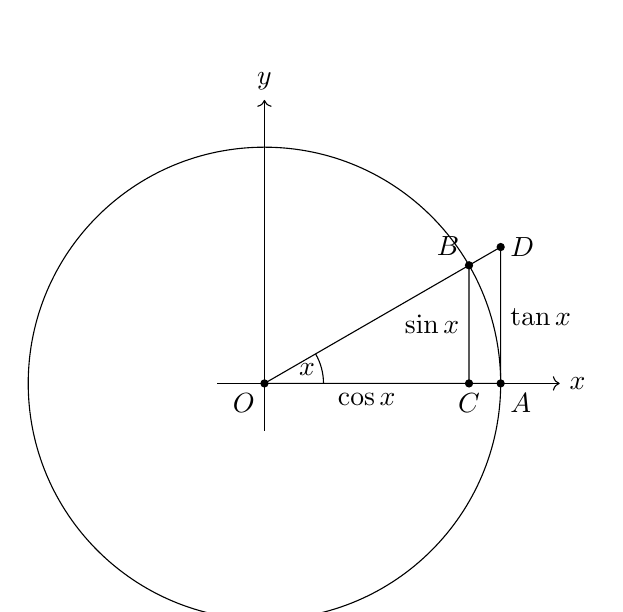
\begin{tikzpicture}[scale=3]
\coordinate (O) at (0,0);
\coordinate (A) at (1,0);
\coordinate (B) at ({cos(30)},{sin(30)});
\coordinate (C) at ({cos(30)},0);
\coordinate (D) at (1,{tan(30)});
\draw[->] (-0.2,0) -- (1.25,0) node[right] {$x$};
\draw[->] (0,-0.2) -- (0,1.2) node[above] {$y$};
\draw (O) circle (1);
\draw (O)--(A) (O)--(D) (B)--(C) (A)--(D);
\fill (O) circle (0.5pt) node[below left] {$O$};
\fill (A) circle (0.5pt) node[below right] {$A$};
\fill (B) circle (0.5pt) node[above left] {$B$};
\fill (C) circle (0.5pt) node[below] {$C$};
\fill (D) circle (0.5pt) node[right] {$D$};
\draw (0.25,0) arc (0:30:0.25);
\node at (0.18,0.06) {$x$};
\node[right] at (1,0.28) {$\tan x$};
\node[left] at ({cos(30)},0.25) {$\sin x$};
\node[below] at ({cos(30)/2},0) {$\cos x$};
\end{tikzpicture}
\end{center}

图中：
\begin{itemize}
\item 角 \(x\) 对应的圆弧长 = \(x\)（因为半径=1，弧长=半径×角度）
\item 垂线 \(BC\) 的长度 = \(\sin x\)
\item 水平线 \(OC\) 的长度 = \(\cos x\)
\item 切线 \(AD\) 的长度 = \(\tan x\)
\end{itemize}

从图中可以看出，三个面积之间有如下关系：

\[
\triangle OAB \text{ 的面积 } < \text{ 扇形 } OAB \text{ 的面积 } < \triangle OAD \text{ 的面积}.
\]

\end{custom}

\begin{custom}{面积比较}

\begin{itemize}
\item \(\triangle OAB\) 的面积 = \(\dfrac{1}{2} \times 1 \times \sin x = \dfrac{1}{2} \sin x\)
\item 扇形 \(OAB\) 的面积 = \(\dfrac{1}{2} \times 1^2 \times x = \dfrac{x}{2}\)
\item \(\triangle OAD\) 的面积 = \(\dfrac{1}{2} \times 1 \times \tan x = \dfrac{1}{2} \tan x\)
\end{itemize}

因此：

\[
\dfrac{1}{2} \sin x  <  \dfrac{x}{2} < \dfrac{1}{2} \tan x \qquad (0 < x < \dfrac{\pi}{2}).
\]

两边同时乘以 2，得到：

\[
\sin x  < x < \tan x.
\]

\end{custom}

\begin{custom}{推导 \(\dfrac{\sin x}{x}\) 的夹逼不等式}

由 \(x < \tan x = \dfrac{\sin x}{\cos x}\)，两边同时除以 \(\sin x > 0\)，得：

\[
\dfrac{x}{\sin x} < \dfrac{1}{\cos x} \quad \Longrightarrow \quad \cos x < \dfrac{\sin x}{x}.
\]

又由 \(\sin x < x\)，两边除以 \(x > 0\)，得：

\[
\dfrac{\sin x}{x} < 1.
\]

合起来：

\[
\cos x < \dfrac{\sin x}{x} < 1 \qquad (0 < x < \dfrac{\pi}{2}).
\]

\end{custom}

\begin{custom}{用夹逼准则取极限}

由 \(|\sin u|\leq|u|\)，有
\[
0\leq1-\cos x=2\sin^2\frac x2\leq\frac{x^2}{2},
\]
所以由夹逼定理可先得到 \(\lim_{x\to0}\cos x=1\)。因此，当 \(x \to 0^+\) 时：

\[
\cos x \;\longrightarrow\; 1,\quad \dfrac{\sin x}{x} \;\longrightarrow\; 1.
\]

当 \(x\) 为负时（即 \(x \to 0^-\)），由于 \(\dfrac{\sin x}{x}\) 是偶函数（\(\sin(-x)/(-x) = \sin x / x\)），左右极限相等。因此：

\[
\lim_{x \to 0} \dfrac{\sin x}{x} = 1.
\]

\end{custom}

\begin{example}
	求 \(\lim_{x \to 0} \dfrac{\sin 2x}{x}\)。
\end{example}

\begin{solution}
	\[
	\dfrac{\sin 2x}{x} = 2 \cdot \dfrac{\sin 2x}{2x} \to 2 \cdot 1 = 2.
	\]
\end{solution}


\begin{application}[物理：小角度近似]

这个极限告诉我们：当角度 \(x\) 非常小时，\(\sin x\) 和 \(x\) 几乎相等。这里的角度必须使用\textbf{弧度}。例如：

\[
x = 0.1 \text{ 弧度} \approx 5.73^\circ,\quad \sin(0.1) \approx 0.099833,\quad \dfrac{\sin 0.1}{0.1} \approx 0.99833.
\]

\[
x = 0.01 \text{ 弧度},\quad \dfrac{\sin 0.01}{0.01} \approx 0.999983.
\]

误差非常小，且随 \(x\) 越小，比值越接近 $1$。这一近似常见于小振幅单摆、光学近轴近似和小角度机械运动。本章只由极限说明近似成立，不提前使用泰勒公式；第6章将进一步估计误差。

\end{application}

\begin{application}[生物医学：饱和响应的低浓度近似]
设教学模型
\[
v(C)=\frac{V_{\max}C}{K+C},\qquad V_{\max}>0,\quad K>0,
\]
其中 $C$ 表示浓度，$v(C)$ 表示响应速率。假设在所研究范围内参数保持不变，则
\[
\frac{v(C)}{C}=\frac{V_{\max}}{K+C}
\longrightarrow\frac{V_{\max}}K
\qquad(C\to0^+).
\]
因此在低浓度范围内，
\[
v(C)\approx\frac{V_{\max}}K\,C.
\]
这说明非线性响应在局部可以近似为线性。本例只用于展示局部近似结构，不应把该公式直接解释为临床剂量关系；具体生物系统还可能存在多种反应途径和参数变化。\upcite{NCBIEnzyme}
\end{application}

\subsubsection*{第二个重要极限}


\begin{theorem}[自然常数 e ]
	\[
	\lim_{n\to\infty} \left(1 + \dfrac{1}{n}\right)^n = \ee.
	\]
\end{theorem}



\begin{custom}{具体证明}
	证明分为两步：先证 \(\{a_n\}\) 单调递增，再证它有上界。
	
	\noindent\textbf{第一步：证明单调递增}
	
	由二项式定理展开：
	\[
	a_n = \left(1+\dfrac{1}{n}\right)^n = \sum\limits_{k=0}^{n} C_n^k \dfrac{1}{n^k} = \sum_{k=0}^{n} \dfrac{1}{k!} \cdot \dfrac{n(n-1)\cdots(n-k+1)}{n^k}.
	\]
	其中 \(\dfrac{n(n-1)\cdots(n-k+1)}{n^k} = 1 \cdot \left(1-\dfrac{1}{n}\right) \cdots \left(1-\dfrac{k-1}{n}\right)\)。于是
	\[
	a_n = \sum_{k=0}^{n} \dfrac{1}{k!} \left(1-\dfrac{1}{n}\right)\left(1-\dfrac{2}{n}\right)\cdots\left(1-\dfrac{k-1}{n}\right).
	\]
	
	同理，
	\[
	a_{n+1} = \sum_{k=0}^{n+1} \dfrac{1}{k!} \left(1-\dfrac{1}{n+1}\right)\left(1-\dfrac{2}{n+1}\right)\cdots\left(1-\dfrac{k-1}{n+1}\right).
	\]
	
	比较 \(a_n\) 与 \(a_{n+1}\) 中 \(k\) 相同的项（\(1 \leq k \leq n\)）：
	\[
	\left(1-\dfrac{1}{n}\right)\left(1-\dfrac{2}{n}\right)\cdots\left(1-\dfrac{k-1}{n}\right) < \left(1-\dfrac{1}{n+1}\right)\left(1-\dfrac{2}{n+1}\right)\cdots\left(1-\dfrac{k-1}{n+1}\right),
	\]
	因为每个因子 \(1-\dfrac{j}{n}<1-\dfrac{j}{n+1}\)（\(j=1,2,\dots,k-1\)），并且 \(a_{n+1}\) 还多出一个正项。因此
	\[
	a_n < a_{n+1},
	\]
	故数列严格递增。
	
	\noindent\textbf{第二步：证明有上界}
	
	由展开式，
	\[
	a_n = \sum_{k=0}^{n} \dfrac{1}{k!} \left(1-\dfrac{1}{n}\right)\cdots\left(1-\dfrac{k-1}{n}\right) \leq \sum_{k=0}^{n} \dfrac{1}{k!}.
	\]
	
	当 \(k \geq 1\) 时，\(k! = 1 \cdot 2 \cdot 3 \cdots k \geq 1 \cdot 2 \cdot 2 \cdots 2 = 2^{k-1}\)，因此
	\[
	\dfrac{1}{k!} \leq \dfrac{1}{2^{k-1}} \quad (k \geq 1).
	\]
	
	于是
	\[
	a_n < 1 + 1 + \dfrac{1}{2} + \dfrac{1}{2^2} + \cdots + \dfrac{1}{2^{n-1}} = 1 + \dfrac{1 - (1/2)^n}{1 - 1/2} = 1 + 2\left(1 - \dfrac{1}{2^n}\right) < 3.
	\]
	
	所以 \(a_n < 3\) 对所有 \(n\) 成立，数列有上界。
	
	\noindent\textbf{结论：} 数列 \(\{a_n\}\) 单调递增且有上界，由单调有界准则，极限存在。记这个极限为 \(\ee\)，即
	\[
	\ee = \lim_{n\to\infty} \left(1+\dfrac{1}{n}\right)^n.
	\]
\end{custom}



\begin{theorem}[第二个重要极限]
\[
\lim_{x\to0}(1+x)^{1/x}=\ee.
\]
\end{theorem}
\begin{proofdetail}
先考虑 \(x\to0^+\)。令
\[
n=\left\lfloor\frac1x\right\rfloor,
\]
则当 \(x\to0^+\) 时 \(n\to\infty\)，并且
\[
\frac1{n+1}<x\leq\frac1n,\qquad n\leq\frac1x<n+1.
\]
由于此时各底数都大于 \(1\)，有
\[
\left(1+\frac1{n+1}\right)^n
\leq(1+x)^{1/x}
\leq\left(1+\frac1n\right)^{n+1}.
\]
记 \(a_n=(1+\frac1n)^n\)。前面已经证明 \(a_n\to\ee\)，而
\[
\left(1+\frac1{n+1}\right)^n
=\frac{a_{n+1}}{1+\frac1{n+1}}\to\ee,
\]
\[
\left(1+\frac1n\right)^{n+1}
=a_n\left(1+\frac1n\right)\to\ee.
\]
由夹逼定理，
\[
\lim_{x\to0^+}(1+x)^{1/x}=\ee.
\]

再考虑 \(x\to0^-\)。当 \(x\) 充分接近 \(0\) 时 \(x>-1\)。令
\[
y=-\frac{x}{1+x},
\]
则 \(y\to0^+\)，且 \(1+x=(1+y)^{-1}\)、\(1/x=-(1+y)/y\)。因此
\[
(1+x)^{1/x}
=(1+y)^{(1+y)/y}
=(1+y)^{1/y}(1+y)\to\ee.
\]
左右极限相等，所以
\[
\lim_{x\to0}(1+x)^{1/x}=\ee.
\]
\end{proofdetail}

\begin{theorem}[第二个重要极限的离散推广]
对任意实数 \(a\)，
\[
\lim_{n\to\infty}\left(1+\frac an\right)^n=\ee^a.
\]
\end{theorem}
\begin{proofdetail}
当 \(a=0\) 时结论显然成立。当 \(a\neq0\) 时，令 \(x=a/n\)，则 \(x\to0\)，且对充分大的 \(n\)，\(1+a/n>0\)。于是
\[
\left(1+\frac an\right)^n
=\left[(1+x)^{1/x}\right]^a\longrightarrow\ee^a.
\]
\end{proofdetail}


\begin{example}
	求 \(\lim\limits_{n\to\infty} \left(1 + \dfrac{2}{n}\right)^n\)。
\end{example}
\begin{solution}
	\[
	\left(1 + \dfrac{2}{n}\right)^n = \left[\left(1 + \dfrac{1}{n/2}\right)^{n/2}\right]^2 \to \ee^2.
	\]
\end{solution}

\subsection{等价无穷小}

在计算极限时，我们经常遇到两个无穷小量相乘或相除的情况。如果能用一个简单的无穷小量代替复杂的无穷小量，计算会大大简化。这就是等价无穷小的思想。

\begin{definition}[无穷小量]
	如果 $\lim _{x \rightarrow a} f(x)=0$ ，那么 $f(x)$ 称为是 $x \rightarrow a$ 时的无穷小量．如果 $f(x)$ 与 $g(x)$都是 $x \rightarrow a$ 时的无穷小量，那么
	\begin{itemize}
		\item[1．] 当 $\lim _{x \rightarrow a} \frac{g(x)}{f(x)}=0$ 时，说 $g(x)$ 是 $f(x)$ 的高阶无穷小，记为 $g(x)=o(f(x))$ ；
		\item[2．] 当 $\lim _{x \rightarrow a} \frac{g(x)}{f(x)}=L>0$ 时，说 $g(x)$ 是 $f(x)$ 的同阶无穷小，特别地，当 $L=1$ 时，称为等价无穷小，记为 $\mathrm{f}(\mathrm{x}) \sim \mathrm{g}(\mathrm{x})$ ；
	\end{itemize}

\end{definition}







\subsubsection{\texorpdfstring{常用等价无穷小（\(x \to 0\) 时）}{常用等价无穷小（x 趋于 0 时）}}

以下等价关系是微积分中最常用的，务必熟记：

\[
\boxed{
\begin{aligned}
\sin x &\sim x & \tan x &\sim x \\
\arcsin x &\sim x & \arctan x &\sim x \\
\ee^x - 1 &\sim x & \ln(1+x) &\sim x \\
1 - \cos x &\sim \dfrac{x^2}{2} & (1+x)^a - 1 &\sim ax \quad (a \neq 0)
\end{aligned}
}
\]

\begin{remark}
本章在处理指数、对数和三角函数时，使用高中阶段已经熟悉的初等函数基本连续性，例如 $\ln x$ 在 $x>0$ 上连续。本章后半部分将用极限语言正式定义函数连续性，并系统讨论一般连续函数的性质。
\end{remark}

\begin{custom}{几个等价关系的推导}

\begin{itemize}
\item \textbf{\(\sin x \sim x\)：} 这就是我们之前证明的 \(\lim_{x \to 0} \dfrac{\sin x}{x} = 1\)。

\item \textbf{\(\tan x \sim x\)：} 
\[
\lim_{x \to 0} \dfrac{\tan x}{x} = \lim_{x \to 0} \dfrac{\sin x}{x} \cdot \dfrac{1}{\cos x} = 1 \cdot 1 = 1.
\]

\item \textbf{\(\ln(1+x)\sim x\)：} 由第二个重要极限及对数函数的连续性，
\[
\lim_{x\to0}\frac{\ln(1+x)}{x}
=\lim_{x\to0}\ln\!\left[(1+x)^{1/x}\right]
=\ln\ee=1.
\]

\item \textbf{\(\ee^x-1\sim x\)：} 令 \(t=\ee^x-1\)，则 \(x=\ln(1+t)\)。当 \(x\to0\) 时 \(t\to0\)，利用刚证明的 \(\ln(1+t)\sim t\)，
\[
\lim_{x\to0}\frac{\ee^x-1}{x}
=\lim_{t\to0}\frac{t}{\ln(1+t)}=1.
\]

\item \textbf{\(1 - \cos x \sim \dfrac{x^2}{2}\)：} 
\[
\lim_{x \to 0} \dfrac{1 - \cos x}{x^2/2} = \lim_{x \to 0} \dfrac{2 \sin^2(x/2)}{x^2/2} = \lim_{x \to 0} \dfrac{4 \sin^2(x/2)}{x^2} = \lim_{x \to 0} \left(\dfrac{\sin(x/2)}{x/2}\right)^2 = 1.
\]

\item \textbf{\((1+x)^a - 1 \sim ax\)：} 
\[
\lim_{x \to 0} \dfrac{(1+x)^a - 1}{ax} = \dfrac{1}{a} \cdot \lim_{x \to 0} \dfrac{\ee^{a\ln(1+x)} - 1}{x} = \dfrac{1}{a} \cdot \lim_{x \to 0} \dfrac{a\ln(1+x)}{x} = 1.
\]
\end{itemize}
\end{custom}

\subsubsection{等价无穷小的应用：简化极限计算}

\begin{custom}{核心原则}
在乘除结构中，可以用等价无穷小替换来简化计算：
\[
\lim \dfrac{f(x)}{g(x)} = \lim \dfrac{\tilde{f}(x)}{\tilde{g}(x)},
\]
其中 \(\tilde{f} \sim f\)，\(\tilde{g} \sim g\)。

\textbf{但注意：} 在加减结构中，不能随意替换！因为主要项可能相互抵消，替换后可能丢失关键信息。
\end{custom}

\begin{example}[乘除结构中的替换]
求 \(\lim\limits_{x \to 0} \dfrac{\sin 2x \cdot \ln(1+3x)}{x^2}\)。
\end{example}
\begin{solution}
当 \(x \to 0\) 时，\(\sin 2x \sim 2x\)，\(\ln(1+3x) \sim 3x\)，所以
\[
\dfrac{\sin 2x \cdot \ln(1+3x)}{x^2} \sim \dfrac{(2x) \cdot (3x)}{x^2} = 6 \quad \Rightarrow \quad \text{极限为 } 6.
\]
更严谨地：
\[
\lim_{x \to 0} \dfrac{\sin 2x \cdot \ln(1+3x)}{x^2} = \lim_{x \to 0} \dfrac{\sin 2x}{2x} \cdot \dfrac{\ln(1+3x)}{3x} \cdot 6 = 1 \cdot 1 \cdot 6 = 6.
\]
\end{solution}

\begin{example}[加减结构的拆分]
求 \(\lim\limits_{x \to 0} \dfrac{\ee^{x^2} - \cos x}{x^2}\)。
\end{example}
\begin{solution}
这里分子是两项相减，不能把 \(\ee^{x^2}\) 与 \(\cos x\) 都直接替换为 \(1\)。将分子按已知等价无穷小拆分：
\[
\frac{\ee^{x^2}-\cos x}{x^2}
=\frac{\ee^{x^2}-1}{x^2}+\frac{1-\cos x}{x^2}.
\]
由于 \(\ee^u-1\sim u\)（取 \(u=x^2\)）且 \(1-\cos x\sim x^2/2\)，所以
\[
\lim_{x\to0}\frac{\ee^{x^2}-\cos x}{x^2}
=1+\frac12=\frac32.
\]

\textbf{注意：} 这里不能直接用 \(\ee^{x^2}\sim1\) 和 \(\cos x\sim1\)，因为 \(1-1=0\) 会丢失主要信息。
\end{solution}

\begin{example}[加减结构中的易错点]
求 \(\lim\limits_{x \to 0} \dfrac{\tan x - \sin x}{x^3}\)。




\begin{solution}
	先用恒等变形把相减结构改写为乘除结构：
	\[
	\frac{\tan x-\sin x}{x^3}
	=\frac{\sin x(1-\cos x)}{x^3\cos x}.
	\]
	利用 \(\sin x\sim x\)、\(1-\cos x\sim x^2/2\) 以及 \(\cos x\to1\)，得到
	\[
	\lim_{x\to0}\frac{\tan x-\sin x}{x^3}
	=\frac12.
	\]
	
\end{solution}

\textbf{注意：} 这里不能直接使用 \(\tan x \sim x\)，\(\sin x \sim x\)，否则 \(\tan x - \sin x \sim x - x = 0\)，极限为 0。


\iffalse

\begin{custom}{后续方法预告}
学习泰勒公式后，也可以写成
\[
\tan x=x+\frac{x^3}{3}+o(x^3),\qquad
\sin x=x-\frac{x^3}{6}+o(x^3),
\]
从而立即看出三次项的系数之差为 \(1/2\)。这里仅作方法预告，不把尚未建立的泰勒公式作为当前证明的依据。
\end{custom}

\fi
\end{example}

\begin{custom}{等价无穷小替换的口诀}
\begin{center}
\fbox{\parbox{0.85\textwidth}{
\textbf{乘除可换因子，加减先防抵消。}\\
\textbf{当前先作恒等变形，学完泰勒公式后再看高阶项。}}
}
\end{center}

\textbf{具体规则：}
\begin{itemize}
\item 在乘除结构中：可以用等价无穷小替换因子。
\item 在加减结构中，不能仅由 $\alpha\sim\widetilde\alpha$、$\beta\sim\widetilde\beta$ 就把各项分别替换后再相加或相减，因为主项可能发生抵消。
\item 若已经证明 $\alpha=o(\beta)$，则
\[
\alpha+\beta
=\beta\left(1+\frac{\alpha}{\beta}\right)
=\beta[1+o(1)]
\sim\beta.
\]
此时可以说高阶项 $\alpha$ 相对于主项 $\beta$ 可以忽略。
\item 若两个无穷小同阶，尤其需要警惕主项抵消；若发生抵消，应使用恒等变形、已知极限或后续的泰勒展开继续分析。“不是同阶”本身也不保证存在明确的高阶关系，例如两个无穷小的比值可能振荡。
\end{itemize}
\end{custom}

\subsubsection{等价无穷小与无穷小量阶的比较}

为了更精确地描述无穷小量趋近于 0 的“速度”，我们引入阶的概念。

\begin{definition}[无穷小的阶]
设 \(\alpha(x) \to 0\)，\(\beta(x) \to 0\)，且 \(\beta(x) \neq 0\)。
\begin{itemize}
\item 若 \(\lim \dfrac{\alpha}{\beta} = 0\)，称 \(\alpha\) 是比 \(\beta\) 高阶的无穷小，记作 \(\alpha = o(\beta)\)。
\item 若 \(\lim \dfrac{\alpha}{\beta} = C \neq 0\)，称 \(\alpha\) 与 \(\beta\) 是同阶无穷小。
\item 特别地，若 \(C = 1\)，称 \(\alpha\) 与 \(\beta\) 是等价无穷小，记作 \(\alpha \sim \beta\)。
\end{itemize}
\end{definition}

\begin{custom}{阶的比较：举例}
当 \(x \to 0\) 时：
\begin{itemize}
\item \(x^2\) 是比 \(x\) 高阶的无穷小：\(\dfrac{x^2}{x} = x \to 0\)，记作 \(x^2 = o(x)\)。
\item \(x^2\) 与 \(2x^2\) 是同阶无穷小：\(\dfrac{x^2}{2x^2} = \dfrac{1}{2}\)。
\item \(x\) 与 \(\sin x\) 是等价无穷小：\(\dfrac{x}{\sin x} \to 1\)。
\end{itemize}

\textbf{阶的比较示意图：}
\[
\underbrace{x^3}_{o(x^2)} \quad \ll \quad \underbrace{x^2}_{o(x)} \quad \ll \quad \underbrace{x}_{\text{一阶}} \quad \ll \quad \underbrace{\sqrt{x}}_{\text{低阶}}
\]
\end{custom}

\Needspace{0.62\textheight}
\begin{extra}
\subsection*{等价无穷小的推广（选读）}


\begin{custom}{推广一：复合函数的等价替换}
若当 \(u \to 0\) 时 \(f(u) \sim g(u)\)，且 \(u(x) \to 0\)，则当 \(x \to x_0\) 时 \(f(u(x)) \sim g(u(x))\)。

例如：\(\sin(x^2) \sim x^2\)（因为 \(x^2 \to 0\)），\(\ln(1+\sin x) \sim \sin x \sim x\)。

\begin{example}
求 \(\lim\limits_{x \to 0} \dfrac{\ln(1 + \sin x)}{x}\)。
\end{example}
\begin{solution}
当 \(x \to 0\) 时，\(\sin x \to 0\)，所以 \(\ln(1+\sin x) \sim \sin x \sim x\)，因此
\[
\lim_{x \to 0} \dfrac{\ln(1+\sin x)}{x} = 1.
\]
\end{solution}
\end{custom}

\begin{custom}{推广二：多个等价无穷小的链式替换}
若 \(\alpha \sim \beta\)，\(\beta \sim \gamma\)，则 \(\alpha \sim \gamma\)。等价关系具有传递性。

例如：\(\ee^x - 1 \sim x \sim \ln(1+x)\)，所以 \(\ee^x - 1 \sim \ln(1+x)\)。
\end{custom}
\end{extra}


\iffalse

\subsection{极限计算与易错分析}

\begin{example}
求 \(\lim_{x \to 0} \dfrac{\sin 2x}{x}\)。
\end{example}

\begin{solution}
\[
\dfrac{\sin 2x}{x} = 2 \cdot \dfrac{\sin 2x}{2x} \to 2 \cdot 1 = 2.
\]
\end{solution}

\begin{example}
求 \(\lim_{x \to 0} \dfrac{1 - \cos x}{x^2}\)。
\end{example}

\begin{solution}
利用 \(1 - \cos x = 2 \sin^2 \dfrac{x}{2}\)：
\[
\dfrac{1 - \cos x}{x^2} = \dfrac{2 \sin^2 \dfrac{x}{2}}{x^2} = \dfrac{1}{2} \cdot \left( \dfrac{\sin (x/2)}{x/2} \right)^2 \to \dfrac{1}{2} \cdot 1^2 = \dfrac{1}{2}.
\]
\end{solution}

\begin{example}
求 \(\lim\limits_{n\to\infty} \left(1 + \dfrac{2}{n}\right)^n\)。
\end{example}
\begin{solution}
\[
\left(1 + \dfrac{2}{n}\right)^n = \left[\left(1 + \dfrac{1}{n/2}\right)^{n/2}\right]^2 \to \ee^2.
\]
\end{solution}

\begin{example}
求 \(\lim\limits_{n\to\infty} \left(\dfrac{n}{n+1}\right)^n\)。
\end{example}
\begin{solution}
\[
\left(\dfrac{n}{n+1}\right)^n = \dfrac{1}{\left(1 + \dfrac{1}{n}\right)^n} \to \dfrac{1}{\ee}.
\]
\end{solution}



\begin{custom}{方法总结：用差分求幂和的大O形式}

上述方法的核心思路：
\[
k^m = \dfrac{1}{m+1} \left[(k+1)^{m+1} - k^{m+1}\right] + O(k^{m-1}).
\]

对其求和得到：
\[
\sum_{k=1}^n k^m
=\frac{n^{m+1}}{m+1}+O(n^m)
\qquad(m\ge1).
\]

这种方法的优点：
\begin{itemize}
\item 不需要记住 \(\sum  k^m\) 的精确公式。
\item 直接得到主要项和误差阶，足以计算极限。
\end{itemize}
\end{custom}

\subsubsection{易错警示：常见极限错误分析}

在学习极限时，初学者常犯的错误是滥用极限的四则运算法则，特别是将“和的极限”与“极限的和”随意混用，或者错误地拆分乘积。下面通过几个典型例子说明这些错误。

\begin{example}[错误：滥用极限的四则运算法则]
求 \(\lim\limits_{n\to\infty} \dfrac{1 + 2 + \cdots + n}{n^2}\)。

\textbf{错误解法（常见错误）：}
\[
\lim_{n\to\infty} \dfrac{1 + 2 + \cdots + n}{n^2} = \lim_{n\to\infty} \dfrac{1}{n^2} + \lim_{n\to\infty} \dfrac{2}{n^2} + \cdots + \lim_{n\to\infty} \dfrac{n}{n^2} = 0 + 0 + \cdots + 0 = 0.
\]

\textbf{为什么错误？}

极限的四则运算法则只适用于\textbf{有限项}的加减乘除。而这里，分子是 \(n\) 个项的和，当 \(n \to \infty\) 时，项数也在趋于无穷。我们不能将“有限项和”的极限法则直接推广到“无限项和”！

换句话说，\(\lim_{n\to\infty} \sum_{k=1}^{n} a_k(n)\) 不能简单地等于 \(\sum_{k=1}^{\infty} \lim_{n\to\infty} a_k(n)\)，除非有额外的条件（如一致收敛）。

\textbf{正确解法：}
先求和，再求极限：
\[
1 + 2 + \cdots + n = \dfrac{n(n+1)}{2},
\]
所以
\[
\lim_{n\to\infty} \dfrac{1 + 2 + \cdots + n}{n^2} = \lim_{n\to\infty} \dfrac{n(n+1)}{2n^2} = \lim_{n\to\infty} \dfrac{1 + 1/n}{2} = \dfrac{1}{2}.
\]

\textbf{结论：} 当分子或分母本身是随 \(n\) 变化的求和（或求积）时，必须先化简，不能逐项取极限。
\end{example}

\begin{example}[错误：拆分乘积中的无穷小量]
求 \(\lim\limits_{n\to\infty} \left(1 + \dfrac{1}{n}\right)^n\)。

\textbf{错误解法（常见错误）：}
\[
\lim_{n\to\infty} \left(1 + \dfrac{1}{n}\right)^n = \left(\lim_{n\to\infty} \left(1 + \dfrac{1}{n}\right)\right)^n = 1^\infty = 1 \quad \text{（错误!）}
\]

\textbf{为什么错误？}

这里的问题在于：指数 \(n\) 本身也在趋于无穷。我们不能先对内层取极限（得到 1），再用这个极限去做无穷次方。\(1^\infty\) 是\textbf{不定式}，不同表达式可能得到不同的有限极限、无穷大或不存在极限，需要具体分析。

正确解法见前文（第一个重要极限）。

\textbf{结论：} 遇到 \(1^\infty\) 型极限，不能直接认为等于 1，要转化为 \((1 + \dfrac{1}{n})^n\) 的形式处理。
\end{example}

\fi

\begin{extra}
\subsection*{Stolz定理（选读）}

Stolz定理可以看作处理某些 \(\dfrac{\infty}{\infty}\) 型数列极限的离散版洛必达法则：
设 \(\{a_n\}, \{b_n\}\) 满足 \(b_n \to +\infty\) 且单调递增，若 \(\lim \dfrac{a_{n+1}-a_n}{b_{n+1}-b_n} = L\)，则 \(\lim \dfrac{a_n}{b_n} = L\)。

例如，用Stolz定理可证 \(\lim_{n\to\infty} \dfrac{\ln n}{n} = 0\)：
\[
\lim_{n\to\infty} \dfrac{\ln n}{n} = \lim_{n\to\infty} \dfrac{\ln(n+1) - \ln n}{(n+1)-n} = \lim_{n\to\infty} \ln\left(1+\dfrac{1}{n}\right) = 0.
\]
\end{extra}

\subsection{一元函数的连续性}

\begin{definition}[函数在一点连续]
设函数 $f$ 在点 $x_0$ 的某邻域内有定义，且 $f(x_0)$ 有定义。 若
\[
\lim_{x\to x_0}f(x)=f(x_0),
\]
则称 $f$ 在点 $x_0$ 处连续。 等价地，对任意 $\varepsilon>0$，存在 $\delta>0$，使得当 $|x-x_0|<\delta$ 且 $x$ 属于函数定义域时，都有
\[
|f(x)-f(x_0)|<\varepsilon.
\]
\end{definition}

\begin{definition}[左右连续]
若
\[
\lim_{x\to x_0-}f(x)=f(x_0),
\]
则称 $f$ 在 $x_0$ 处左连续；若
\[
\lim_{x\to x_0+}f(x)=f(x_0),
\]
则称 $f$ 在 $x_0$ 处右连续。 函数在 $x_0$ 连续，当且仅当它在 $x_0$ 左连续且右连续。
\end{definition}

\begin{definition}[区间上的连续]
若 $f$ 在开区间 $(a,b)$ 内每一点连续，则称 $f$ 在 $(a,b)$ 上连续。 若 $f$ 在 $(a,b)$ 内连续，且
\[
\lim_{x\to a+}f(x)=f(a),\qquad \lim_{x\to b-}f(x)=f(b),
\]
则称 $f$ 在闭区间 $[a,b]$ 上连续。
\end{definition}

\begin{center}
\begin{tikzpicture}[scale=0.9,>=Stealth]
  \draw[->] (-0.3,0)--(5.8,0) node[right] {$x$};
  \draw[->] (0,-0.3)--(0,3.2) node[above] {$y$};
  \draw[domain=0.3:5.2,smooth,variable=\x,thick] plot ({\x},{1.4+0.35*sin(80*\x)});
  \node at (2.9,-0.55) {连续图像：局部变化不会出现跳跃};
\end{tikzpicture}
\qquad
\begin{tikzpicture}[scale=0.9,>=Stealth]
  \draw[->] (-0.3,0)--(5.8,0) node[right] {$x$};
  \draw[->] (0,-0.3)--(0,3.2) node[above] {$y$};
  \draw[domain=0.3:2.65,smooth,variable=\x,thick] plot ({\x},{0.7+0.25*\x});
  \draw[domain=2.75:5.2,smooth,variable=\x,thick] plot ({\x},{1.8+0.12*(\x-3)^2});
  \filldraw[white] (2.7,1.375) circle (2.2pt);
  \draw (2.7,1.375) circle (2.2pt);
  \fill (2.7,1.81) circle (2.2pt);
  \node at (2.9,-0.55) {不连续图像：极限值与函数值不一致};
\end{tikzpicture}
\end{center}


\begin{proposition}[四则运算]
若 $f,g$ 在 $x_0$ 处连续，则 $f+g,\,f-g,\,fg$ 在 $x_0$ 处连续。 若 $g(x_0)\neq0$，则 $\frac{f}{g}$ 在 $x_0$ 处连续。
\end{proposition}
\begin{proofdetail}
以乘积为例。 由连续性得
\[
\lim_{x\to x_0}f(x)=f(x_0),\qquad \lim_{x\to x_0}g(x)=g(x_0).
\]
由极限乘法法则，
\[
\lim_{x\to x_0}f(x)g(x)=f(x_0)g(x_0),
\]
故 $fg$ 在 $x_0$ 连续。 加、减同理。 对商函数，由 $g(x_0)\neq0$ 且 $g$ 连续，存在 $x_0$ 的某邻域使 $g(x)\neq0$，于是商函数在该邻域有定义，并由极限商法则得
\[
\lim_{x\to x_0}\frac{f(x)}{g(x)}=\frac{f(x_0)}{g(x_0)}.
\]
故 $\frac{f}{g}$ 连续。
\end{proofdetail}

\begin{proposition}[复合函数连续性]
若 $g$ 在 $x_0$ 处连续，$f$ 在 $g(x_0)$ 处连续，则复合函数 $f\circ g$ 在 $x_0$ 处连续。
\end{proposition}
\begin{proofdetail}
记 $y_0=g(x_0)$。 给定任意 $\varepsilon>0$。 因 $f$ 在 $y_0$ 处连续，存在 $\eta>0$，使得当 $|y-y_0|<\eta$ 时，
\[
|f(y)-f(y_0)|<\varepsilon.
\]
因 $g$ 在 $x_0$ 处连续，存在 $\delta>0$，使得当 $|x-x_0|<\delta$ 时，
\[
|g(x)-g(x_0)|<\eta.
\]
于是当 $|x-x_0|<\delta$ 时，
\[
|f(g(x))-f(g(x_0))|<\varepsilon.
\]
这正是 $f\circ g$ 在 $x_0$ 处连续。
\end{proofdetail}



\begin{definition}[间断点]
若 $f$ 在 $x_0$ 不连续，则称 $x_0$ 为 $f$ 的间断点。 常见情形包括：
\begin{enumerate}[label=(\arabic*),leftmargin=2em]
\item 可去间断：$\lim_{x\to x_0}f(x)$ 存在，但不等于 $f(x_0)$，或 $f(x_0)$ 未定义；
\item 跳跃间断：左右极限都存在但不相等；
\item 无穷间断：至少有一个单侧极限为 \(+\infty\) 或 \(-\infty\)；
\item 振荡间断：函数在该点附近无限振荡，极限不存在。
\end{enumerate}
\end{definition}

\begin{example}
讨论函数
\[
f(x)=
\begin{cases}
\dfrac{\sin x}{x},&x\neq0,\\
a,&x=0
\end{cases}
\]
在 $x=0$ 处的连续性。
\end{example}
\begin{solution}
因为
\[
\lim_{x\to0}\frac{\sin x}{x}=1,
\]
所以 $f$ 在 $0$ 处连续当且仅当 $a=1$。 若 $a\neq1$，极限存在但不等于函数值，$0$ 是可去间断点。
\end{solution}
\begin{warning}
分段函数在分段点处必须检查左极限、右极限和函数值三者。 只检查表达式能否代入，不能保证连续。
\end{warning}

\iffalse
\begin{example}
设
\[
f(x)=
\begin{cases}
x^2+1,&x<1,\\
ax+b,&x\ge1.
\end{cases}
\]
求 $a,b$ 的条件，使 $f$ 在 $x=1$ 连续；若还要求左右导数相等，求 $a,b$。
\end{example}
\begin{solution}
连续要求
\[
\lim_{x\to1-}f(x)=f(1).
\]
左极限为 $2$，右侧函数值 $f(1)=a+b$，故连续条件为
\[
a+b=2.
\]
若还要求左右导数相等，左侧导数为 $(x^2+1)'|_{x=1}=2$，右侧导数为 $a$，故 $a=2$。 代入连续条件得 $b=0$。
\end{solution}
\fi



\subsection*{闭区间连续函数的两个基本定理}

\begin{theorem}[有界性与最值定理]
若 $f$ 在闭区间 $[a,b]$ 上连续，则 $f$ 在 $[a,b]$ 上有界，并且存在 $x_m,x_M\in[a,b]$，使得
\[
f(x_m)\le f(x)\le f(x_M)\qquad (x\in[a,b]).
\]
\end{theorem}
\begin{proofdetail}
先证有界性。 若 $f$ 无界，则对每个正整数 $n$，可取 $x_n\in[a,b]$ 使 $|f(x_n)|>n$。 数列 $\{x_n\}$ 有界，故存在收敛子列 $x_{n_k}\to x_0\in[a,b]$。 由于 $f$ 在 $x_0$ 连续，有 $f(x_{n_k})\to f(x_0)$，于是 $\{f(x_{n_k})\}$ 有界。 但 $|f(x_{n_k})|>n_k\to\infty$，矛盾。 故 $f$ 有界。

设
\[
M=\sup\{f(x):x\in[a,b]\}.
\]
由上确界定义，对每个 $n$ 存在 $x_n\in[a,b]$，使
\[
M-\frac1n<f(x_n)\le M.
\]
取收敛子列 $x_{n_k}\to x_M\in[a,b]$。 连续性给出
\[
f(x_M)=\lim_{k\to\infty}f(x_{n_k})=M.
\]
故最大值取到。 对 $-f$ 应用同样结论，可得最小值取到。
\end{proofdetail}

\begin{theorem}[介值定理]
若 $f$ 在 $[a,b]$ 上连续，且 $N$ 介于 $f(a)$ 与 $f(b)$ 之间，则存在 $\xi\in[a,b]$，使得
\[
f(\xi)=N.
\]
\end{theorem}
\begin{proofdetail}
不妨设 $f(a)<N<f(b)$。 令
\[
S=\{x\in[a,b]:f(x)<N\}.
\]
则 $S$ 非空且有上界。 设 $\xi=\sup S$。 若 $f(\xi)>N$，由连续性可得 $\xi$ 左侧足够近的点也满足 $f(x)>N$，这与 $\xi$ 是 $S$ 的上确界矛盾。 若 $f(\xi)<N$，由连续性可得 $\xi$ 右侧足够近的点仍满足 $f(x)<N$，这与 $\xi$ 是 $S$ 的上界矛盾；若 $\xi=b$，则与 $f(b)>N$ 矛盾。 因此只能有 $f(\xi)=N$。
\end{proofdetail}

\begin{example}
证明方程 $x^3+x-1=0$ 在 $(0,1)$ 内至少有一个实根。
\end{example}
\begin{solution}
令 $f(x)=x^3+x-1$。 多项式函数在 $[0,1]$ 上连续。 有
\[
f(0)=-1,\qquad f(1)=1.
\]
由于 $0$ 介于 $f(0)$ 与 $f(1)$ 之间，由介值定理，存在 $\xi\in(0,1)$，使 $f(\xi)=0$。 因而方程在 $(0,1)$ 内至少有一个实根。
\end{solution}

\begin{example}
某商品价格为 $p$ 时的需求量模型为 $Q(p)=120-5p$，其中 $p$ 的单位为元，$Q$ 的单位为件。 若价格从 $12$ 元连续调整到 $20$ 元，问是否存在某个价格使需求量恰好为 $40$ 件？
\end{example}
\begin{solution}
这里的“需求函数” $Q(p)$ 表示价格 $p$ 与消费者愿意购买数量之间的函数关系。 模型 $Q(p)=120-5p$ 为一次函数，因此在 $[12,20]$ 上连续。 有
\[
Q(12)=60,\qquad Q(20)=20.
\]
由于 $40$ 介于 $20$ 与 $60$ 之间，介值定理保证存在 $\xi\in[12,20]$，使 $Q(\xi)=40$。 直接求解 $120-5\xi=40$，得 $\xi=16$。
\end{solution}

\begin{application}[工程：传感器标定与介值定理]
设压力传感器的输出电压为 $V(P)$，其中压力 $P$ 的单位为 $\mathrm{kPa}$，电压 $V$ 的单位为 $\mathrm V$。假设在量程 $100\leq P\leq200$ 内，传感器响应连续，并已测得
\[
V(100)=2.1\ \mathrm V,\qquad V(200)=3.7\ \mathrm V.
\]
目标电压 $3.0\ \mathrm V$ 介于两个端点输出之间。因此由介值定理，至少存在一个
\[
P_*\in(100,200)
\]
使 $V(P_*)=3.0\ \mathrm V$。介值定理只保证目标状态存在；若要确定 $P_*$ 的数值，还需要更具体的标定函数或数值测量。实际传感器还可能有噪声、滞后和量化误差，本例只讨论理想的连续响应。
\end{application}

\begin{application}[农业：田间含水率阈值]
沿一条长 $100\ \mathrm m$ 的田间测线，以 $x$ 表示距起点的位置，以 $M(x)$ 表示体积含水率。假设忽略局部土质突变，并用连续函数近似空间变化。若
\[
M(0)=12\%,\qquad M(100)=28\%,
\]
而灌溉管理阈值为 $20\%$，则存在 $x_*\in(0,100)$ 使 $M(x_*)=20\%$。这说明测线上必有位置达到阈值，但不说明该位置唯一。真实田间数据来自离散采样，并受土壤结构、地形和天气影响；连续性是用于说明介值定理的教学假设。\upcite{BradyWeil}
\end{application}


\subsection{二元函数的极限与连续}

一元函数中，\(x\to x_0\) 只有从左、从右两种基本方向；在平面上，点 \((x,y)\) 可以沿直线、曲线或其他任意路径趋近 \((x_0,y_0)\)。因此，二元函数的极限必须对所有趋近方式给出同一个结果。

\begin{definition}[二元函数的极限]
	设函数 \(f(x,y)\) 在点 \(P_0=(x_0,y_0)\) 的某个去心邻域内有定义。记
	\[
	\rho=\sqrt{(x-x_0)^2+(y-y_0)^2}.
	\]
	若存在常数 \(A\)，使得对任意 \(\varepsilon>0\)，总存在 \(\delta>0\)，当
	\[
	0<\rho<\delta
	\]
	时都有
	\[
	|f(x,y)-A|<\varepsilon,
	\]
	则称当 \((x,y)\to(x_0,y_0)\) 时 \(f(x,y)\) 的极限为 \(A\)，记作
	\[
	\lim_{(x,y)\to(x_0,y_0)}f(x,y)=A.
	\]
\end{definition}

\begin{example}[按定义证明二元极限]
	证明
	\[
	\lim_{(x,y)\to(0,0)}(x^2+y^2)=0.
	\]
\end{example}
\begin{proofdetail}
	任取 \(\varepsilon>0\)，取 \(\delta=\sqrt{\varepsilon}\)。当
	\[
	0<\sqrt{x^2+y^2}<\delta
	\]
	时，
	\[
	|(x^2+y^2)-0|=x^2+y^2<\delta^2=\varepsilon.
	\]
	因此该极限为 \(0\)。
\end{proofdetail}

\begin{custom}{用不同路径判定极限不存在}
	若二元极限存在，则沿任意一条趋近目标点的路径，函数值都必须趋于同一结果。因此，只要找到两条路径得到不同的极限，就能断定二元极限不存在。
\end{custom}

\begin{example}[两条路径给出不同结果]
	考察
	\[
	\lim_{(x,y)\to(0,0)}\frac{xy}{x^2+y^2}.
	\]
	沿 \(y=0\) 趋近时，
	\[
	\frac{x\cdot0}{x^2+0}=0;
	\]
	沿 \(y=x\) 趋近时，
	\[
	\frac{x^2}{x^2+x^2}=\frac12\qquad(x\neq0).
	\]
	两条路径得到的结果不同，所以该二元极限不存在。
\end{example}

\begin{warning}
	检查若干条直线路径只能用来发现极限不存在，不能据此证明极限存在。例如
	\[
	f(x,y)=\frac{x^2y}{x^4+y^2}.
	\]
	沿每条直线 \(y=mx\) 都有
	\[
	f(x,mx)=\frac{mx}{x^2+m^2}\to0
	\]
	（\(m=0\) 时也成立），但沿抛物线 \(y=x^2\) 有
	\[
	f(x,x^2)=\frac12.
	\]
	因此，即使所有直线路径给出相同结果，也仍可能存在其他曲线路径给出不同结果。
\end{warning}

\begin{theorem}[二元函数极限的基本运算法则]
	若
	\[
	\lim_{(x,y)\to(x_0,y_0)}f(x,y)=A,\qquad
	\lim_{(x,y)\to(x_0,y_0)}g(x,y)=B,
	\]
	则和、差、积的极限分别为 \(A+B\)、\(A-B\)、\(AB\)；当 \(B\neq0\) 时，商的极限为 \(A/B\)。二元函数的极限也具有唯一性、局部有界性、保号性和夹逼性质。
\end{theorem}

\begin{definition}[二元函数的连续性]
	若 \(f(x,y)\) 在点 \((x_0,y_0)\) 有定义，并且
	\[
	\lim_{(x,y)\to(x_0,y_0)}f(x,y)=f(x_0,y_0),
	\]
	则称 \(f\) 在 \((x_0,y_0)\) 连续。若 \(f\) 在区域 \(D\) 内每一点都连续，则称 \(f\) 在 \(D\) 上连续。
\end{definition}

\begin{proposition}[连续函数的运算]
	二元连续函数的和、差、积仍连续；分母不为零时，商也连续。多项式函数在整个平面上连续，有理函数在分母不为零的点连续；由连续初等函数经过有限次四则运算与复合所得的二元函数，在其定义域内连续。
\end{proposition}

\begin{example}[利用连续性求极限]
	求
	\[
	\lim_{(x,y)\to(1,2)}
	\frac{x^2+\sin(xy)}{x+y}.
	\]
\end{example}
\begin{solution}
	分子、分母均为连续函数，且目标点处分母 \(1+2=3\neq0\)，所以可直接代入：
	\[
	\lim_{(x,y)\to(1,2)}
	\frac{x^2+\sin(xy)}{x+y}
	=\frac{1+\sin2}{3}.
	\]
\end{solution}




\iffalse

\subsection*{第4章课后习题}
\addcontentsline{toc}{subsection}{第4章课后习题}

\subsubsection*{第4.1--4.6节\quad 函数极限}

\begin{exercise}求下列极限：
\begin{enumerate}
\item \(\lim\limits_{n\to\infty} \dfrac{3n^2 - 2n + 1}{n^2 + 5}\)
\item \(\lim\limits_{n\to\infty} \left(\dfrac{2n-1}{3n+2} + \dfrac{n+1}{4n-3}\right)\)
\item \(\lim\limits_{n\to\infty} \dfrac{\sqrt{n^2 + 3n} - n}{2}\)
\end{enumerate}
\end{exercise}

\begin{exercise}用夹逼准则求下列极限：
\begin{enumerate}
\item \(\lim\limits_{n\to\infty} \dfrac{\sin n}{n}\)
\item \(\lim\limits_{n\to\infty} \left(\dfrac{1}{n^2+1} + \dfrac{1}{n^2+2} + \cdots + \dfrac{1}{n^2+n}\right)\)
\end{enumerate}
\end{exercise}

\begin{exercise}求下列极限：
\begin{enumerate}
\item \(\lim\limits_{n\to\infty} \left(1 + \dfrac{3}{n}\right)^n\)
\item \(\lim\limits_{n\to\infty} \left(1 - \dfrac{1}{n}\right)^n\)
\item \(\lim\limits_{x\to 0} \dfrac{\sin 3x}{x}\)
\item \(\lim\limits_{x\to 0} \dfrac{1 - \cos x}{x^2}\)
\end{enumerate}
\end{exercise}

\begin{exercise}求下列极限：
\begin{enumerate}
\item \(\lim\limits_{x\to 0} \dfrac{\tan 2x}{\sin 5x}\)
\item \(\lim\limits_{x\to 0} \dfrac{\ee^{2x} - 1}{\ln(1+3x)}\)
\item \(\lim\limits_{x\to 0} \dfrac{\ln(1 + x^2)}{x \sin x}\)
\end{enumerate}
\end{exercise}

\begin{exercise}[改错题：找出下面解法的错误并改正]
求 \(\lim\limits_{n\to\infty} \dfrac{1 + 2 + \cdots + n}{n^2 + 1}\)。

\textbf{错误解法：}
\[
\lim_{n\to\infty} \dfrac{1 + 2 + \cdots + n}{n^2 + 1} = \lim_{n\to\infty} \dfrac{1}{n^2+1} + \lim_{n\to\infty} \dfrac{2}{n^2+1} + \cdots + \lim_{n\to\infty} \dfrac{n}{n^2+1} = 0 + 0 + \cdots + 0 = 0.
\]

请指出错误原因，并写出正确解法。
\end{exercise}

\begin{exercise}[改错题：找出下面解法的错误并改正]
求 \(\lim\limits_{n\to\infty} \left(1 + \dfrac{1}{n}\right)^{2n}\)。

\textbf{错误解法：}
\[
\lim_{n\to\infty} \left(1 + \dfrac{1}{n}\right)^{2n} = \left(\lim_{n\to\infty} \left(1 + \dfrac{1}{n}\right)\right)^{2n} = 1 ^{2n}=1.
\]

\textbf{另一位同学的解法：}
\[
\lim_{n\to\infty} \left(1 + \dfrac{1}{n}\right)^{2n} = \lim_{n\to\infty} \left(\left(1 + \dfrac{1}{n}\right)^n\right)^2 = \ee^2.
\]

请问第一位同学的解法错在哪里？第二位同学的解法正确吗？为什么？
\end{exercise}

\begin{exercise}[改错题：找出下面解法的错误并改正]
求 \(\lim\limits_{x\to 0} \dfrac{\tan x - \sin x}{x^3}\)。

\textbf{错误解法：}
由于 \(\tan x \sim x\)、\(\sin x\sim x\)（当 \(x \to 0\)），所以 \(\tan x-\sin x\sim x-x=0\)，因此原极限 \(=0\)。

请指出错误原因，并给出正确解法。
\end{exercise}

\begin{exercise}已知 \(\lim\limits_{n\to\infty} a_n = 2\)，\(\lim\limits_{n\to\infty} b_n = -1\)，求下列极限：
\begin{enumerate}
\item \(\lim\limits_{n\to\infty} (3a_n - 2b_n)\)
\item \(\lim\limits_{n\to\infty} (a_n b_n + 2a_n)\)
\item \(\lim\limits_{n\to\infty} \dfrac{a_n^2 - b_n}{a_n + b_n}\)
\end{enumerate}
\end{exercise}

\begin{exercise}判断下列说法是否正确，正确的请简要说明理由，错误的请举反例：
\begin{enumerate}
\item 有界数列一定收敛。
\item 收敛数列一定有界。
\item 若 \(\lim a_n = 0\)，则 \(\{a_n\}\) 是无穷小量。
\item 若 \(\{a_n\}\) 是无穷大量，则 \(\{a_n\}\) 无界。
\item 若 \(\{a_n\}\) 无界，则 \(\{a_n\}\) 是无穷大量。
\end{enumerate}
\end{exercise}

\begin{exercise}求下列极限：
\begin{enumerate}
\item \(\lim\limits_{n\to\infty} \left(1 + \dfrac{1}{2n}\right)^n\)
\item \(\lim\limits_{n\to\infty} \left(\dfrac{n+1}{n-1}\right)^n\)
\item \(\lim\limits_{x\to 0} (1 + 2x)^{\dfrac{1}{x}}\)
\end{enumerate}
\end{exercise}

\subsubsection*{第4.7--4.10节\quad 函数的连续性}

\begin{enumerate}[label=\textbf{练习\arabic*.},leftmargin=2.2em]
\item 求常数 $a$，使
\[
f(x)=
\begin{cases}
\dfrac{1-\cos x}{x^2},&x\neq0,\\
a,&x=0
\end{cases}
\]
在 $x=0$ 连续。
\item 讨论函数 $f(x)=\frac{x^2-1}{x-1}$ 在 $x=1$ 处的间断类型，并说明如何补充定义使其连续。
\item 证明方程 $\cos x=x$ 在 $(0,1)$ 内至少有一个实根。
\item 设成本函数 $C(x)=100+20x+0.5x^2$，价格函数 $p(x)=80-0.2x$。 若收益 $R(x)=xp(x)$，利润 $P(x)=R(x)-C(x)$，说明 $P$ 在 $[0,100]$ 上是否一定能取到最大值。
\end{enumerate}

\subsection*{第4章参考答案与提示}
\addcontentsline{toc}{subsection}{第4章参考答案与提示}

\subsubsection*{第4.1--4.6节\quad 函数极限}

\begin{enumerate}
\item[1.] 
   (a) \(3\) \quad (b) \(\dfrac{2}{3} + \dfrac{1}{4} = \dfrac{11}{12}\) \quad (c) \(\dfrac{3}{4}\)（先分子有理化：\(\sqrt{n^2+3n} - n = \dfrac{3n}{\sqrt{n^2+3n}+n} \to \dfrac{3}{2}\)，再除以2得 \(\dfrac{3}{4}\)）

\item[2.] 
   (a) \(0\)（\(-\dfrac{1}{n} \leq \dfrac{\sin n}{n} \leq \dfrac{1}{n}\)）\quad 
   (b) \(0\)（\(\dfrac{n}{n^2+n} \leq \text{原式} \leq \dfrac{n}{n^2+1}\)）

\item[3.] 
(a) \(\ee^3\) \quad (b) \(\dfrac{1}{\ee}\) \quad (c) \(3\) \quad (d) \(\dfrac{1}{2}\)

\item[4.] 
   (a) \(\dfrac{2}{5}\) \quad (b) \(\dfrac{2}{3}\) \quad (c) \(1\)

\item[5.] 
   \textbf{错误原因：} 极限的四则运算法则只适用于有限项，这里分子有 \(n\) 项，项数随 \(n\) 变化，不能逐项取极限。
   
   \textbf{正确解法：} \(1+2+\cdots+n = \dfrac{n(n+1)}{2}\)，所以原式 \(= \lim\limits_{n\to\infty} \dfrac{n(n+1)}{2(n^2+1)} = \lim\limits_{n\to\infty} \dfrac{1+1/n}{2(1+1/n^2)} = \dfrac{1}{2}\)。

\item[6.] 
   第一位同学的解法错误：他先对括号内取极限得1，然后做 \(1^{2n}\) 次方得1，这是错误的，因为 \(1^\infty\) 是不定式，不能先算括号内再算指数。
   
第二位同学的解法正确：因为 \(\left(1+\dfrac{1}{n}\right)^{2n} = \left[\left(1+\dfrac{1}{n}\right)^n\right]^2\)，而括号内极限为 \(\ee\)，平方后得 \(\ee^2\)。注意这里的指数 \(2n\) 是整体指数，不能拆成先极限再指数。

\item[7.] 
   \textbf{错误原因：} 等价无穷小替换在加减法中不能直接使用。\(\tan x\) 和 \(\sin x\) 的主要项相同，相减后主要项发生抵消。
   
   \textbf{正确解法：}
   \[
   \frac{\tan x-\sin x}{x^3}
   =\frac{\sin x}{x}\cdot\frac{1-\cos x}{x^2}\cdot\frac1{\cos x}
   \longrightarrow 1\cdot\frac12\cdot1=\frac12.
   \]

\item[8.] 
   (a) \(3 \times 2 - 2 \times (-1) = 6 + 2 = 8\) \quad
   (b) \(2 \times (-1) + 2 \times 2 = -2 + 4 = 2\) \quad
   (c) \(\dfrac{4 - (-1)}{2 + (-1)} = \dfrac{5}{1} = 5\)

\item[9.] 
   (a) 错误，反例：\(a_n = (-1)^n\) 有界但不收敛。\quad
   (b) 正确，收敛数列必有界。\quad
   (c) 正确，无穷小量的定义就是极限为 0。\quad
   (d) 正确，无穷大量一定无界。\quad
   (e) 错误，反例：\(a_n = n(1+(-1)^n)\) 无界但不是无穷大量（奇数项为 0，偶数项为 \(2n\)）。

\item[10.] 
(a) \(\lim\left(1+\dfrac{1}{2n}\right)^n = \lim\left[\left(1+\dfrac{1}{2n}\right)^{2n}\right]^{1/2} = \ee^{1/2} = \sqrt{\ee}\) \quad
   (b) \(\left(\dfrac{n+1}{n-1}\right)^n = \left(1 + \dfrac{2}{n-1}\right)^n = \left(1 + \dfrac{2}{n-1}\right)^{n-1} \cdot \left(1 + \dfrac{2}{n-1}\right) \to \ee^2 \cdot 1 = \ee^2\) \quad
   (c) \(\lim (1+2x)^{1/x} = \lim \left[(1+2x)^{\dfrac{1}{2x}}\right]^2 = \ee^2\)
\end{enumerate}

连续性连接了极限与导数。 直观地说，函数在一点连续表示当自变量发生足够小的变化时，函数值也只发生足够小的变化；几何上表现为图像在该点没有跳跃、空洞或爆裂。 但在大学数学中，仅靠图像直观是不够的，连续性必须由极限严格定义。

\subsubsection*{第4.7--4.10节\quad 函数的连续性}

\begin{enumerate}[label=\textbf{练习\arabic*.},leftmargin=2.2em]
\item 因 $\lim_{x\to0}\frac{1-\cos x}{x^2}=\frac12$，故 $a=\frac12$。
\item 当 $x\neq1$ 时 $f(x)=x+1$，故 $\lim_{x\to1}f(x)=2$，但原函数在 $x=1$ 未定义。 这是可去间断点。 定义 $f(1)=2$ 后函数在 $x=1$ 连续。
\item 令 $F(x)=\cos x-x$。 $F$ 在 $[0,1]$ 上连续，且 $F(0)=1>0$，$F(1)=\cos1-1<0$。 由介值定理，存在 $\xi\in(0,1)$ 使 $F(\xi)=0$。
\item $P(x)=x(80-0.2x)-(100+20x+0.5x^2)$ 是多项式函数，故在 $[0,100]$ 上连续。 由闭区间连续函数最值定理，$P$ 在 $[0,100]$ 上一定能取到最大值和最小值。
\end{enumerate}

\fi

\clearpage
\section{导数的概念与计算}

本章讨论一元函数微分学的起点：导数。 在前面学习极限与连续时，我们已经能够描述“函数值是否趋近某个数”“函数图像是否断开”。 但在许多问题中，仅知道函数连续是不够的；还需要知道变量变化得快还是慢、曲线在一点附近朝哪个方向延伸、经济变量在当前水平下继续增加一个单位会带来多大影响。 这些问题都指向同一个数学对象：函数改变量与自变量改变量之比的极限。


\subsection{导数的概念}
\subsubsection*{从变化率到导数}

微分学研究变量变化的快慢。 按照常见教材的处理，导数可以从两个典型问题抽象出来。

\begin{definition}[平均变化率]
设函数 $y=f(x)$ 在区间 $[x_1,x_2]$ 上有定义，且 $x_1\neq x_2$。 比值
\[
\frac{f(x_2)-f(x_1)}{x_2-x_1}
\]
称为 $f$ 在 $[x_1,x_2]$ 上的平均变化率。 若记 $x_2=x_1+\Delta x$，则平均变化率也可写成
\[
\frac{\Delta y}{\Delta x}
=\frac{f(x_1+\Delta x)-f(x_1)}{\Delta x}.
\]
它描述的是函数值在一段区间上的平均增减速度。
\end{definition}

第一，设物体作直线运动，路程为 $s=s(t)$。 在时间区间 $[t_0,t_0+\Delta t]$ 上的平均速度为
\[
\frac{\Delta s}{\Delta t}
=\frac{s(t_0+\Delta t)-s(t_0)}{\Delta t}.
\]
当 $\Delta t\to0$ 时，若这个平均速度有极限，则该极限定义为时刻 $t_0$ 的瞬时速度。

第二，设曲线为 $y=f(x)$，曲线上两点 $(x_0,f(x_0))$ 与 $(x_0+\Delta x,f(x_0+\Delta x))$ 所确定割线的斜率为
\[
\frac{\Delta y}{\Delta x}
=\frac{f(x_0+\Delta x)-f(x_0)}{\Delta x}.
\]
当 $\Delta x\to0$ 时，若割线斜率有极限，则该极限就是曲线在点 $(x_0,f(x_0))$ 处切线的斜率。 两个问题的共同数学形式都是“函数改变量与自变量改变量之比的极限”，这就是导数。

\begin{center}
\begin{tikzpicture}[scale=1.0,>=Stealth]
  \draw[->] (-0.2,0)--(5.4,0) node[right] {$x$};
  \draw[->] (0,-0.2)--(0,3.6) node[above] {$y$};
  \draw[domain=0.45:4.75,smooth,variable=\x,thick]
    plot ({\x},{0.16*(\x-2.2)*(\x-2.2)+0.8});
  \coordinate (M) at (2.0,0.806);
  \coordinate (P) at (4.0,1.318);
  \fill (M) circle (1.5pt) node[below left] {$M_0$};
  \fill (P) circle (1.5pt) node[above right] {$M$};
  \draw[thick,dashed] ($(M)!-0.45!(P)$)--($(M)!1.35!(P)$) node[right] {割线};
  \draw[thick] ($(M)+(-1.05,-0.067)$)--($(M)+(1.35,0.086)$) node[right] {切线};
  \draw[dashed] (M)--(2.0,0) node[below] {$x_0$};
  \draw[dashed] (P)--(4.0,0) node[below] {$x_0+\Delta x$};
  \node at (3.05,0.45) {$\Delta x$};
  \node at (4.35,1.05) {$\Delta y$};
\end{tikzpicture}
\end{center}

\begin{example}[平均速度与瞬时速度]
设自由落体的路程函数为
\[
s(t)=\frac12gt^2,
\]
其中 $g>0$ 为重力加速度。 求 $t_0$ 到 $t_0+\Delta t$ 这段时间内的平均速度，并求时刻 $t_0$ 的瞬时速度。
\end{example}
\begin{solution}
平均速度为
\[
\frac{s(t_0+\Delta t)-s(t_0)}{\Delta t}
=\frac{\frac12g(t_0+\Delta t)^2-\frac12gt_0^2}{\Delta t}
=gt_0+\frac12g\Delta t.
\]
令 $\Delta t\to0$，得瞬时速度
\[
v(t_0)=\lim_{\Delta t\to0}\left(gt_0+\frac12g\Delta t\right)=gt_0.
\]
这个例子说明：平均速度依赖一段时间，而瞬时速度是平均速度在时间间隔收缩到 $0$ 时的极限。
\end{solution}

\begin{definition}[导数]
设函数 $f$ 在点 $x_0$ 的某邻域内有定义。 若极限
\[
\lim_{\Delta x\to0}\frac{f(x_0+\Delta x)-f(x_0)}{\Delta x}
\]
存在且为有限实数，则称 $f$ 在 $x_0$ 处可导，并称该极限为 $f$ 在 $x_0$ 处的导数，记作
\[
f'(x_0),\quad \left.\frac{\dd y}{\dd x}\right|_{x=x_0},\quad \left.\frac{\dd f}{\dd x}\right|_{x=x_0}.
\]
若上述极限不存在，则称 $f$ 在 $x_0$ 处不可导。 若差商趋于无穷大，本讲义不把它称为有限导数；有些教材会说该点“导数为无穷大”，其含义是切线为垂直方向，而不是导数作为实数存在。
\end{definition}

令 $x=x_0+\Delta x$，导数定义也可写成
\[
f'(x_0)=\lim_{x\to x_0}\frac{f(x)-f(x_0)}{x-x_0}.
\]

\begin{definition}[左导数与右导数]
若
\[
f'_-(x_0)=\lim_{\Delta x\to0-}\frac{f(x_0+\Delta x)-f(x_0)}{\Delta x},\quad
f'_+(x_0)=\lim_{\Delta x\to0+}\frac{f(x_0+\Delta x)-f(x_0)}{\Delta x}
\]
存在，则分别称为左导数与右导数。
\end{definition}

\begin{proposition}[可导的充要条件]
$f$ 在 $x_0$ 处可导，当且仅当 $f'_-(x_0)$ 与 $f'_+(x_0)$ 都存在且相等。 此时共同值等于 $f'(x_0)$。
\end{proposition}
\begin{proofdetail}
这是函数极限左右极限判别准则在差商函数
\[
\varphi(\Delta x)=\frac{f(x_0+\Delta x)-f(x_0)}{\Delta x}\quad(\Delta x\neq0)
\]
上的直接应用。 若 $\lim_{\Delta x\to0}\varphi(\Delta x)$ 存在，则左右极限存在且等于该极限。 反过来，若左右极限均存在且相等，记共同值为 $A$，则由一元函数极限存在的左右极限定理，$\lim_{\Delta x\to0}\varphi(\Delta x)=A$，故 $f'(x_0)=A$。
\end{proofdetail}

\begin{theorem}[可导必连续]
若 $f$ 在 $x_0$ 处可导，则 $f$ 在 $x_0$ 处连续。
\end{theorem}
\begin{proofdetail}
对 $x\neq x_0$，写成
\[
f(x)-f(x_0)=\frac{f(x)-f(x_0)}{x-x_0}(x-x_0).
\]
令 $x\to x_0$。 因 $f$ 在 $x_0$ 可导，
\[
\lim_{x\to x_0}\frac{f(x)-f(x_0)}{x-x_0}=f'(x_0)
\]
为有限数，而 $\lim_{x\to x_0}(x-x_0)=0$。 由极限乘法法则，
\[
\lim_{x\to x_0}[f(x)-f(x_0)]=f'(x_0)\cdot0=0.
\]
于是 $\lim_{x\to x_0}f(x)=f(x_0)$，即 $f$ 在 $x_0$ 连续。
\end{proofdetail}

\begin{example}[用定义求导]
用导数定义求 函数 $f(x) = ax^2 + bx + c$ 在 $x_0$ 处的导数。
\end{example}
\begin{solution}
根据导数的定义，函数 $f(x) = ax^2 + bx + c$ 在 $x_0$ 处的导数为：

\begin{align*}
	f'(x_0) &= \lim_{\Delta x \to 0} \frac{f(x_0 + \Delta x) - f(x_0)}{\Delta x} \\
	&= \lim_{\Delta x \to 0} \frac{[a(x_0 + \Delta x)^2 + b(x_0 + \Delta x) + c] - (ax_0^2 + bx_0 + c)}{\Delta x} \\
	&= \lim_{\Delta x \to 0} \frac{a(x_0^2 + 2x_0\Delta x + (\Delta x)^2) + bx_0 + b\Delta x + c - ax_0^2 - bx_0 - c}{\Delta x} \\
	&= \lim_{\Delta x \to 0} \frac{2ax_0\Delta x + a(\Delta x)^2 + b\Delta x}{\Delta x} \\
	&= \lim_{\Delta x \to 0} \frac{\Delta x(2ax_0 + a\Delta x + b)}{\Delta x} \\
	&= \lim_{\Delta x \to 0} (2ax_0 + a\Delta x + b) \\
	&= 2ax_0 + b
\end{align*}
\end{solution}
\begin{idea}
定义法的关键是先做代数化简，使差商中的 $\Delta x$ 可以约去，然后再取极限。
\end{idea}

\begin{example}[用定义求根式函数的导数]
用定义求 $f(x)=\sqrt{x}$ 在 $x_0>0$ 处的导数。
\end{example}
\begin{solution}
当 $\Delta x$ 足够小时 $x_0+\Delta x>0$。 差商为
\[
\frac{\sqrt{x_0+\Delta x}-\sqrt{x_0}}{\Delta x}.
\]
分子有根式差，先有理化：
\[
\frac{\sqrt{x_0+\Delta x}-\sqrt{x_0}}{\Delta x}
=\frac{(\sqrt{x_0+\Delta x}-\sqrt{x_0})(\sqrt{x_0+\Delta x}+\sqrt{x_0})}{\Delta x(\sqrt{x_0+\Delta x}+\sqrt{x_0})}
=\frac1{\sqrt{x_0+\Delta x}+\sqrt{x_0}}.
\]
令 $\Delta x\to0$，得
\[
f'(x_0)=\frac1{2\sqrt{x_0}}.
\]
\end{solution}
\begin{idea}
含根式的定义法求导常用有理化。 这一步不是技巧炫耀，而是为了把分子中隐藏的 $\Delta x$ 提取出来。
\end{idea}

\begin{example}[连续但不可导]
证明 $f(x)=|x|$ 在 $0$ 处连续但不可导。
\end{example}
\begin{solution}
连续性：$\lim_{x\to0}|x|=0=f(0)$。

左、右导数分别为
\[
f'_-(0)=\lim_{\Delta x\to0-}\frac{|\Delta x|-0}{\Delta x}
=\lim_{\Delta x\to0-}\frac{-\Delta x}{\Delta x}=-1,
\]
\[
f'_+(0)=\lim_{\Delta x\to0+}\frac{|\Delta x|-0}{\Delta x}
=\lim_{\Delta x\to0+}\frac{\Delta x}{\Delta x}=1.
\]
左右导数不相等，故 $f$ 在 $0$ 处不可导。
\end{solution}

\begin{example}[竖切线与有限导数]
讨论 $f(x)=\sqrt[3]{x}$ 在 $0$ 处的可导性。
\end{example}
\begin{solution}
$f$ 在 $0$ 处连续，因为 $\lim_{x\to0}\sqrt[3]{x}=0=f(0)$。 其差商为
\[
\frac{f(0+h)-f(0)}{h}=\frac{\sqrt[3]{h}}{h}=\frac1{h^{2/3}}.
\]
当 $h\to0$ 时，$\frac1{h^{2/3}}\to+\infty$，不存在有限实数极限。 因此 $f$ 在 $0$ 处不可导。

从图像上看，曲线 $y=\sqrt[3]{x}$ 在原点处有竖直切线。 本讲义中“可导”要求导数为有限实数，所以竖直切线不算可导。
\end{solution}

\begin{example}[分段函数在衔接点的导数]
设
\[
f(x)=
\begin{cases}
x,&x<0,\\
\sin x,&x\geq0.
\end{cases}
\]
求 $f'(0)$。
\end{example}
\begin{solution}
$f(0)=0$。 当 $\Delta x<0$ 时，
\[
\frac{f(0+\Delta x)-f(0)}{\Delta x}=\frac{\Delta x}{\Delta x}=1.
\]
当 $\Delta x>0$ 时，
\[
\frac{f(0+\Delta x)-f(0)}{\Delta x}=\frac{\sin\Delta x}{\Delta x}\to1.
\]
左右差商极限都存在且相等，所以 $f'(0)=1$。
\end{solution}
\begin{warning}
分段函数在分界点处求导，必须使用同一个函数值 $f(0)$ 分别计算左、右差商；不能只对两侧表达式分别求导后直接代入。
\end{warning}

\begin{example}[边际成本]
若总成本函数为 $C(q)=200+5q+0.02q^2$，求产量 $q=100$ 时的边际成本，并解释含义。
\end{example}
\begin{solution}
边际成本是总成本对产量的导数：
\[
C'(q)=5+0.04q,\qquad C'(100)=9.
\]
含义是：在产量 $100$ 附近，产量增加 $1$ 个单位时，总成本约增加 $9$ 个成本单位。 这是局部线性近似，不等于任意大幅增产时的平均增量。
\end{solution}

\begin{definition}[边际函数]
在经济学中，“边际”通常指一个经济变量对另一个经济变量的瞬时变化率。 设产量或销售量为 $x$。

常见经济函数包括：
\begin{itemize}[leftmargin=2em]
\item 成本函数 $C(x)$：生产 $x$ 单位产品所需总成本；
\item 收入函数 $R(x)$：销售 $x$ 单位产品获得的总收入；
\item 利润函数 $L(x)$：总收入减总成本，即 $L(x)=R(x)-C(x)$；
\item 需求函数 $x=Q(p)$：价格为 $p$ 时市场需求量为 $Q(p)$；
\item 反需求函数 $p=p(x)$：销售量为 $x$ 时对应的价格。 若收入按销售量表示，则通常有 $R(x)=xp(x)$。
\end{itemize}

若总成本为 $C=C(x)$，则
\[
C'(x)=\lim_{\Delta x\to0}\frac{C(x+\Delta x)-C(x)}{\Delta x}
\]
称为产量为 $x$ 时的边际成本。 当 $\Delta x$ 较小时，
\[
C(x+\Delta x)-C(x)\approx C'(x)\Delta x.
\]
特别地，当产量单位取得合适时，$C'(x)$ 常被解释为“在产量 $x$ 附近再生产一个单位产品所增加的成本”的近似值。

若总收入为 $R=R(x)$，则 $R'(x)$ 称为边际收入；若总利润为 $L=L(x)$，则 $L'(x)$ 称为边际利润。 由于
\[
L(x)=R(x)-C(x),
\]
只要 $R,C$ 可导，就有
\[
L'(x)=R'(x)-C'(x),
\]
即边际利润等于边际收入减边际成本。
\end{definition}

\begin{definition}[弹性]
设经济变量 $y=f(x)$ 可导，且 $x\neq0,\ f(x)\neq0$。 比值
\[
\frac{\Delta y/f(x)}{\Delta x/x}
\]
称为从 $x$ 到 $x+\Delta x$ 的弧弹性；若极限存在，则
\[
E_y^x(x)=\lim_{\Delta x\to0}\frac{\Delta y/f(x)}{\Delta x/x}
=\frac{x}{f(x)}f'(x)
\]
称为 $y=f(x)$ 在点 $x$ 处关于 $x$ 的点弹性。 弹性刻画的是相对变化率：$x$ 变化 $1\%$ 时，$y$ 近似变化百分之几。 它不依赖变量所采用的具体计量单位。
\end{definition}

从数学上看，边际函数就是导数，弹性则是经过无量纲化的导数。 二者都来自局部线性近似：
\[
f(x+\Delta x)-f(x)\approx f'(x)\Delta x.
\]

\begin{example}[需求价格弹性]
设某商品需求函数为 $Q(p)=400-100p$，其中 $p$ 为价格，$Q$ 为需求量。 求 $p=1,2,3$ 时的需求价格弹性，并解释结果。
\end{example}
\begin{solution}
由定义，
\[
E_Q^p(p)=\frac{p}{Q(p)}Q'(p)=\frac{p}{400-100p}(-100)=-\frac{p}{4-p}.
\]
因此
\[
E_Q^p(1)=-\frac13,\qquad E_Q^p(2)=-1,\qquad E_Q^p(3)=-3.
\]
负号表示价格上升时需求下降。 从绝对值看，$p=1$ 时 $|E|<1$，需求对价格低弹性；$p=2$ 时 $|E|=1$，为单位弹性；$p=3$ 时 $|E|>1$，需求对价格高弹性。 这里的结论完全来自函数的相对变化率，不需要附加虚构情境。
\end{solution}

\begin{example}[边际成本、边际收入与边际利润]
某厂每月固定成本为 $1000$ 元，生产 $x$ 单位产品的可变成本为
\[
0.01x^2+10x
\]
元，每单位产品售价为 $30$ 元。 求边际成本、利润函数，并求边际利润为零时的产量。
\end{example}
\begin{solution}
总成本为固定成本与可变成本之和：
\[
C(x)=0.01x^2+10x+1000.
\]
因此边际成本为
\[
C'(x)=0.02x+10.
\]
总收入为
\[
R(x)=30x.
\]
利润函数为
\[
L(x)=R(x)-C(x)=30x-(0.01x^2+10x+1000)
=-0.01x^2+20x-1000.
\]
边际利润为
\[
L'(x)=-0.02x+20.
\]
令 $L'(x)=0$，得
\[
-0.02x+20=0,\qquad x=1000.
\]
这说明当月产量为 $1000$ 单位时，利润函数的瞬时变化率为零；若进一步结合二阶导数或单调性，可判断这是利润由增转减的临界产量。
\end{solution}

\begin{example}[需求函数与边际收入]
设某产品的需求函数为
\[
x=100-5p,
\]
其中 $p$ 为价格，$x$ 为需求量。 求收入函数 $R(x)$、边际收入函数 $R'(x)$，并解释 $x=20,50,70$ 时的边际收入。
\end{example}
\begin{solution}
由需求函数解出反需求函数：
\[
p=20-\frac{x}{5}.
\]
收入等于价格乘以销量，故
\[
R(x)=xp=x\left(20-\frac{x}{5}\right)=20x-\frac{x^2}{5}.
\]
边际收入为
\[
R'(x)=20-\frac{2x}{5}.
\]
于是
\[
R'(20)=12,\qquad R'(50)=0,\qquad R'(70)=-8.
\]
其含义是：当销售量为 $20$ 时，附近再多销售一个单位，总收入约增加 $12$；当销售量为 $50$ 时，收入的瞬时变化率为 $0$，处于由增转减的临界状态；当销售量为 $70$ 时，再多销售一个单位反而使总收入约减少 $8$。
\end{solution}

\begin{center}
\small
\begin{tabularx}{\textwidth}{>{\bfseries}p{1.4cm} p{2.0cm} X}
\toprule
专业 & 函数 & 导数的含义 \\
\midrule
物理 & $s(t)$ & $s'(t)$：瞬时速度，若 $[s]=\mathrm m$、$[t]=\mathrm s$，则单位为 $\mathrm{m/s}$ \\
工程 & $V(t)$ & $V'(t)$：体积流量，单位可为 $\mathrm{m^3/h}$ \\
农业 & $H(t)$ & $H'(t)$：作物高度的瞬时生长率 \\
医学 & $C(t)$ & $C'(t)$：浓度随时间的瞬时变化率 \\
\bottomrule
\end{tabularx}
\end{center}

导数是“瞬时变化率”的统一数学语言；不同学科改变的是变量的实际含义，而不是极限定义和运算法则。应用中应同时记录变量单位，因为导数的单位等于“因变量单位除以自变量单位”。


\begin{application}[导数与梯度下降的基本思想]
	
	导数还可以解释机器学习中最常见的优化步骤。 在监督学习中，模型含有参数，训练的目标通常是让损失函数尽量小。 损失函数衡量预测值与真实值之间的差距；例如一元线性模型 $\hat y=wx$ 对单个样本 $(x,y)$ 的平方损失可以写成
	\[
	L(w)=\frac12(wx-y)^2.
	\]
	这里 $w$ 是待学习参数，$L(w)$ 是关于参数的函数。 若 $L'(w)>0$，则在 $w$ 附近增大 $w$ 会使损失增大，减小 $w$ 有助于降低损失；若 $L'(w)<0$，则增大 $w$ 有助于降低损失。 因此，一维梯度下降更新为
	\[
	w_{k+1}=w_k-\eta L'(w_k),
	\]
	其中 $\eta>0$ 称为学习率。
	
	\begin{example}
		设损失函数 $L(w)=\frac12(w-3)^2$。 用梯度下降
		\[
		w_{k+1}=w_k-\eta L'(w_k)
		\]
		讨论 $0<\eta<2$ 时 $w_k$ 是否收敛到最小点。
	\end{example}
	\begin{solution}
		先求导：
		\[
		L'(w)=w-3.
		\]
		因此
		\[
		w_{k+1}=w_k-\eta(w_k-3)=(1-\eta)w_k+3\eta.
		\]
		两边同时减去 $3$，得
		\[
		w_{k+1}-3=(1-\eta)(w_k-3).
		\]
		递推得到
		\[
		w_k-3=(1-\eta)^k(w_0-3).
		\]
		当 $0<\eta<2$ 时，$|1-\eta|<1$，所以 $(1-\eta)^k\to0$，于是 $w_k\to3$。 这说明学习率过大可能破坏收敛，而合适的学习率使参数逐步靠近损失函数的最小点。
	\end{solution}
	
\end{application}


\subsubsection*{导数的几何意义}

\begin{definition}[切线与法线]
若 $f$ 在 $x_0$ 处可导，则曲线 $y=f(x)$ 在点 $(x_0,f(x_0))$ 的切线斜率为 $f'(x_0)$，切线方程为
\[
y-f(x_0)=f'(x_0)(x-x_0).
\]
若 $f'(x_0)\neq0$，法线斜率为 $-1/f'(x_0)$，法线方程为
\[
y-f(x_0)=-\frac{1}{f'(x_0)}(x-x_0).
\]
若 $f'(x_0)=0$，切线水平，法线为直线 $x=x_0$。
\end{definition}

\begin{definition}[导函数]
若 $f$ 在区间 $I$ 中每一点可导，则可定义新函数
\[
f':I\to\RR,\qquad x\mapsto f'(x),
\]
称为 $f$ 的导函数。
\end{definition}

\begin{example}[切线与法线]
求抛物线 $y=x^2$ 在点 $(-1,1)$ 处的切线方程和法线方程。
\end{example}
\begin{solution}
由 $y'=2x$，在 $x=-1$ 处切线斜率为 $-2$。 切线方程为
\[
y-1=-2(x+1),
\]
即
\[
2x+y+1=0.
\]
法线斜率为 $-\frac1{-2}=\frac12$，故法线方程为
\[
y-1=\frac12(x+1),
\]
即
\[
x-2y+3=0.
\]
\end{solution}

\begin{example}[切线与参数]
求 $a$，使曲线 $y=x^3+ax$ 在 $x=1$ 处的切线经过点 $(0,0)$。
\end{example}
\begin{solution}
$f(1)=1+a,\ f'(x)=3x^2+a$，故 $f'(1)=3+a$。 切线为
\[
y-(1+a)=(3+a)(x-1).
\]
代入 $(0,0)$ 得
\[
-(1+a)=-(3+a),
\]
即 $1+a=3+a$，矛盾。 因此不存在这样的 $a$。
\end{solution}
\begin{warning}
本题不是所有带参数题都有解。 参数同时出现在点坐标和斜率中，代入条件后必须接受方程无解的可能。
\end{warning}

\begin{example}[由切线条件反求函数值]
设 $f$ 在 $1$ 处可导，且
\[
\lim_{x\to1}\frac{xf(1)-f(x)}{x-1}=2.
\]
求 $f(1)$ 与 $f'(1)$ 的关系。
\end{example}
\begin{solution}
将分子拆为
\[
xf(1)-f(x)=(x-1)f(1)+f(1)-f(x).
\]
因此
\[
\frac{xf(1)-f(x)}{x-1}
=f(1)-\frac{f(x)-f(1)}{x-1}.
\]
令 $x\to1$，由 $f$ 在 $1$ 处可导，得到
\[
2=f(1)-f'(1).
\]
故 $f(1)-f'(1)=2$。
\end{solution}

\subsection{导数的计算}


\subsubsection*{线性组合、积、商与复合函数求导}

最常见的函数是由若干简单函数通过加减、常数倍、乘除和复合构成的。 求导时先辨认函数结构，再选择相应法则。 例如
\[
(3x^2-1)^5
\]
不是幂函数 $x^5$，而是由 $u=3x^2-1$ 与 $y=u^5$ 复合而成；这类问题需要链式法则。

\begin{theorem}[函数线性组合、积、商的求导法则]
若 $u,v$ 在 $x$ 处可导，$a,b$ 为常数，则
\[
[au+bv]'(x)=au'(x)+bv'(x),
\]
\[
(uv)'(x)=u'(x)v(x)+u(x)v'(x).
\]
若 $v(x)\neq0$，则
\[
\left(\frac{u}{v}\right)'(x)=\frac{u'(x)v(x)-u(x)v'(x)}{v^2(x)}.
\]
\end{theorem}
\begin{proofdetail}
先证线性组合。 对任意足够小的 $h\neq0$，
\[
\frac{[au+bv](x+h)-[au+bv](x)}{h}
=a\frac{u(x+h)-u(x)}{h}
+b\frac{v(x+h)-v(x)}{h}.
\]
令 $h\to0$，由 $u,v$ 在 $x$ 处可导以及极限的线性运算法则，得到
\[
[au+bv]'(x)=au'(x)+bv'(x).
\]

再证乘法公式：
\[
\frac{u(x+h)v(x+h)-u(x)v(x)}{h}
=\frac{[u(x+h)-u(x)]v(x+h)}{h}+u(x)\frac{v(x+h)-v(x)}{h}.
\]
令 $h\to0$。 可导必连续，所以 $v(x+h)\to v(x)$。 于是极限为
\[
u'(x)v(x)+u(x)v'(x).
\]
商法可由 $\frac{u}{v}=u\cdot\frac1v$ 推出。 先求
\[
\frac{\frac1{v(x+h)}-\frac1{v(x)}}{h}
=-\frac{v(x+h)-v(x)}{h\,v(x+h)v(x)}.
\]
因 $v(x)\neq0$ 且 $v$ 连续，$h$ 足够小时 $v(x+h)\neq0$，令 $h\to0$ 得 $(1/v)'(x)=-v'(x)/v^2(x)$。 再用乘法法则得商法公式。
\end{proofdetail}

\begin{example}[线性组合求导]
求
\[
y=3x^2+4\ln x-5\cos x,\qquad x>0
\]
的导数。
\end{example}
\begin{solution}
该函数由幂函数、对数函数、三角函数作线性组合得到。 逐项求导：
\[
y'=3\cdot 2x+4\cdot\frac1x-5(-\sin x)
=6x+\frac4x+5\sin x.
\]
这里要求 $x>0$，是因为 $\ln x$ 只在正数上有定义。
\end{solution}

\begin{example}[乘积与商的求导]
求
\[
y=\frac{x^2\sin x}{1+x^2}
\]
的导数。
\end{example}
\begin{solution}
先把分子看作乘积 $u=x^2\sin x$，则
\[
u'=2x\sin x+x^2\cos x.
\]
再对 $y=u/(1+x^2)$ 用商法：
\[
y'=\frac{(2x\sin x+x^2\cos x)(1+x^2)-x^2\sin x\cdot2x}{(1+x^2)^2}.
\]
若需要化简，可展开并合并含 $\sin x$ 的项：
\[
y'=\frac{2x\sin x+x^2\cos x+x^4\cos x}{(1+x^2)^2}.
\]
\end{solution}
\begin{warning}
乘积求导不能写成 $(uv)'=u'v'$。 商求导也不是分子导数除以分母导数。 这两个错误都可以用简单例子检验：若 $u=v=x$，则 $(uv)'=(x^2)'=2x$，而 $u'v'=1$。
\end{warning}

\begin{theorem}[复合函数求导法则]
设 $u=g(x)$ 在 $x$ 处可导，$y=f(u)$ 在 $u_0=g(x)$ 处可导，则复合函数 $f(g(x))$ 在 $x$ 处可导，且
\[
(f\circ g)'(x)=f'(g(x))g'(x).
\]
\end{theorem}
\begin{proofdetail}
由 $f$ 在 $u_0$ 处可导，存在函数 $\alpha(\Delta u)$，满足 $\lim_{\Delta u\to0}\alpha(\Delta u)=0$，使得
\[
f(u_0+\Delta u)-f(u_0)=f'(u_0)\Delta u+\alpha(\Delta u)\Delta u.
\]
这是因为当 $\Delta u\neq0$ 时可令
\[
\alpha(\Delta u)=\frac{f(u_0+\Delta u)-f(u_0)}{\Delta u}-f'(u_0),
\]
并定义 $\alpha(0)=0$。 令 $\Delta u=g(x+h)-g(x)$。 由于 $g$ 在 $x$ 可导，所以 $g$ 在 $x$ 连续，故 $h\to0$ 时 $\Delta u\to0$。 于是
\[
f(g(x+h))-f(g(x))
=\bigl[f'(u_0)+\alpha(\Delta u)\bigr]\,[g(x+h)-g(x)].
\]
两边除以 $h$，令 $h\to0$，得
\[
\lim_{h\to0}\frac{f(g(x+h))-f(g(x))}{h}
=\bigl[f'(u_0)+0\bigr]g'(x).
\]
\end{proofdetail}

\begin{center}
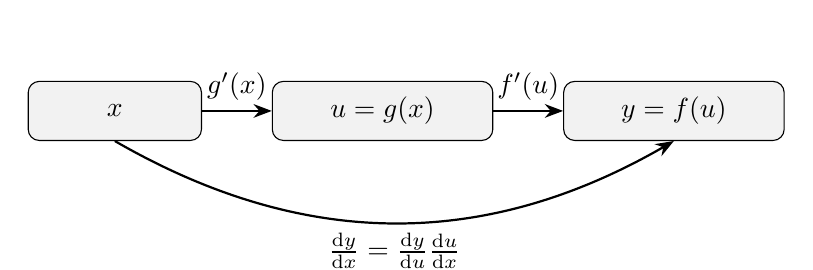
\begin{tikzpicture}[>=Stealth,scale=1.0]
  \node[draw,rounded corners,fill=gray!10,minimum width=2.2cm,minimum height=0.75cm] (x) at (0,0) {$x$};
  \node[draw,rounded corners,fill=gray!10,minimum width=2.8cm,minimum height=0.75cm] (u) at (3.4,0) {$u=g(x)$};
  \node[draw,rounded corners,fill=gray!10,minimum width=2.8cm,minimum height=0.75cm] (y) at (7.1,0) {$y=f(u)$};
  \draw[->,thick] (x) -- node[above] {$g'(x)$} (u);
  \draw[->,thick] (u) -- node[above] {$f'(u)$} (y);
  \draw[->,thick,bend right=30] (x.south) to node[below] {$\frac{\dd y}{\dd x}=\frac{\dd y}{\dd u}\frac{\dd u}{\dd x}$} (y.south);
\end{tikzpicture}
\end{center}

\begin{remark}
链式法则的关键是分清“外层函数”和“内层函数”。 若 $y=f(u)$、$u=g(x)$，则先对外层变量 $u$ 求导，再乘以内层对 $x$ 的导数。 多层复合时逐层相乘。
\end{remark}





\subsubsection*{反函数求导}

有些函数本身不是由初等四则运算直接给出，而是作为另一个函数的反函数出现。 例如 $\ln x$ 是 $\ee^x$ 的反函数，$\arcsin x$ 是适当限制定义域后的 $\sin x$ 的反函数。 反函数求导公式说明：若 $y=f(x)$ 可反解为 $x=\varphi(y)$，则反函数图像在对应点的切线斜率等于原函数切线斜率的倒数。

\begin{theorem}[反函数求导公式]
设 $y=f(x)$ 在点 $x_0$ 的某邻域内严格单调、连续，且 $f$ 在 $x_0$ 处可导，$f'(x_0)\neq0$。 设反函数为 $x=\varphi(y)$，$y_0=f(x_0)$。 若 $\varphi$ 在 $y_0$ 处连续，则 $\varphi$ 在 $y_0$ 处可导，且
\[
\varphi'(y_0)=\frac{1}{f'(x_0)}.
\]
\end{theorem}
\begin{proofdetail}
当 $\Delta y\neq0$ 时，由严格单调性知对应的 $\Delta x=\varphi(y_0+\Delta y)-\varphi(y_0)$ 也不为 $0$，并且
\[
\frac{\Delta x}{\Delta y}
=\frac{1}{\frac{f(x_0+\Delta x)-f(x_0)}{\Delta x}}.
\]
由 $\varphi$ 在 $y_0$ 连续，$\Delta y\to0$ 时 $\Delta x\to0$。 因 $f'(x_0)\neq0$，
\[
\lim_{\Delta y\to0}\frac{\Delta x}{\Delta y}
=\frac{1}{\lim_{\Delta x\to0}\frac{f(x_0+\Delta x)-f(x_0)}{\Delta x}}
=\frac1{f'(x_0)}.
\]
故反函数在 $y_0$ 处可导，公式成立。
\end{proofdetail}

\begin{example}[由反函数推出对数函数导数]
由 $y=\log_a x\ (a>0,\ a\neq1,\ x>0)$，推出其导数公式。
\end{example}
\begin{solution}
令 $y=\log_a x$，则 $x=a^y$。 把 $x$ 看成 $y$ 的函数，有
\[
\frac{\dd x}{\dd y}=a^y\ln a=x\ln a.
\]
由反函数求导公式，
\[
\frac{\dd y}{\dd x}
=\frac{1}{\dd x/\dd y}
=\frac{1}{x\ln a}.
\]
当 $a=\ee$ 时得到
\[
(\ln x)'=\frac1x.
\]
\end{solution}

\begin{example}[反三角函数导数]
求 $y=\arcsin x$ 与 $y=\arctan x$ 的导数。
\end{example}
\begin{solution}
若 $y=\arcsin x$，则
\[
x=\sin y,\qquad y\in\left[-\frac{\pi}{2},\frac{\pi}{2}\right].
\]
在 $|x|<1$ 时，$\cos y>0$，故
\[
\frac{\dd x}{\dd y}=\cos y=\sqrt{1-\sin^2y}=\sqrt{1-x^2}.
\]
由反函数求导公式，
\[
(\arcsin x)'=\frac{1}{\sqrt{1-x^2}},\qquad |x|<1.
\]

若 $y=\arctan x$，则 $x=\tan y$，$y\in(-\pi/2,\pi/2)$。 因而
\[
\frac{\dd x}{\dd y}=\sec^2y=1+\tan^2y=1+x^2,
\]
所以
\[
(\arctan x)'=\frac1{1+x^2},\qquad x\in\RR.
\]
\end{solution}


\begin{proposition}[常用基本导数公式]
	在相应定义域内，下列公式成立。 其中 $a>0,\ a\neq1$；对一般实数 $\alpha$，公式 $(x^\alpha)'=\alpha x^{\alpha-1}$ 通常在 $x>0$ 上使用，若 $\alpha$ 为整数或有理数，还需按函数本身的定义域作相应调整。
	\[
	(C)'=0,\quad (x^\alpha)'=\alpha x^{\alpha-1},\quad (a^x)'=a^x\ln a,\quad (\ee^x)'=\ee^x,
	\]
	\[
	(\log_a |x|)'=\frac1{x\ln a},\quad (\ln |x|)'=\frac1x,
	\]
	\[
	(\sin x)'=\cos x,\quad (\cos x)'=-\sin x,\quad
	(\tan x)'=\sec^2x,\quad (\cot x)'=-\csc^2x,
	\]
	\[
	(\sec x)'=\sec x\tan x,\quad (\csc x)'=-\csc x\cot x,
	\]
	\[
	(\arcsin x)'=\frac1{\sqrt{1-x^2}},\quad
	(\arccos x)'=-\frac1{\sqrt{1-x^2}},
	\]
	\[
	(\arctan x)'=\frac1{1+x^2},\quad
	(\operatorname{arccot}x)'=-\frac1{1+x^2}.
	\]
\end{proposition}remark
\begin{remark}
	这些公式是求导计算的基础。 不宜只背公式：三角函数公式来自导数定义与基本极限，指数与反三角函数公式分别依赖反函数求导和链式法则。以下是灵活运用各种求导法则的例子。
\end{remark}


\begin{example}[公式求导]
	求 $y=(3x^2-1)^5$ 的导数。
\end{example}
\begin{solution}
	令 $u=3x^2-1$，$y=u^5$。 由链式法则
	\[
	y'=5(3x^2-1)^4\cdot6x=30x(3x^2-1)^4.
	\]
\end{solution}

\begin{example}[多层复合求导]
	求
	\[
	y=\ee^{\sqrt{x}},\qquad x>0
	\]
	的导数。
\end{example}
\begin{solution}
	这里有两层复合：
	\[
	x\longmapsto \sqrt{x}\longmapsto \ee^{\sqrt{x}}.
	\]
	因此
	\[
	y'=\ee^{\sqrt{x}}\cdot(\sqrt{x})'
	=\ee^{\sqrt{x}}\cdot\frac{1}{2\sqrt{x}}
	=\frac{\ee^{\sqrt{x}}}{2\sqrt{x}}.
	\]
	在 $x=0$ 处函数有定义，但上述导数公式不适用；事实上右差商趋于无穷大，因此在通常有限导数意义下不可导。
\end{solution}

\begin{example}[复合与乘积同时出现]
	求
	\[
	y=\ee^{-x}\sin\sqrt{2x},\qquad x>0
	\]
	的导数。
\end{example}
\begin{solution}
	这是两个函数的乘积，其中第二个函数又是复合函数。 由乘积法则，
	\[
	y'=(-\ee^{-x})\sin\sqrt{2x}
	+\ee^{-x}\cdot\frac{\dd}{\dd x}\sin\sqrt{2x}.
	\]
	对第二项用链式法则：
	\[
	\frac{\dd}{\dd x}\sin\sqrt{2x}
	=\cos\sqrt{2x}\cdot\frac{\dd}{\dd x}(2x)^{1/2}
	=\cos\sqrt{2x}\cdot\frac1{\sqrt{2x}}.
	\]
	故
	\[
	y'=\ee^{-x}\left(\frac{\cos\sqrt{2x}}{\sqrt{2x}}-\sin\sqrt{2x}\right).
	\]
\end{solution}

\begin{example}[对数求导]
	求 $y=x^x\ (x>0)$ 的导数。
\end{example}
\begin{solution}
	取对数得 $\ln y=x\ln x$。 两边求导：
	\[
	\frac{y'}{y}=\ln x+1.
	\]
	因此
	\[
	y'=x^x(\ln x+1).
	\]
\end{solution}
\begin{warning}
	$x^x$ 不能直接套用幂函数 $x^a$ 或指数函数 $a^x$ 的公式，因为底数和指数都含 $x$。
\end{warning}

\begin{example}[变底变指数函数]
	求
	\[
	y=(\cot x)^{\cos x}
	\]
	的导数，其中在所讨论的区间内 $\cot x>0$。
\end{example}
\begin{solution}
	由于底数和指数都含 $x$，采用对数求导。 取对数：
	\[
	\ln y=\cos x\ln(\cot x).
	\]
	两边对 $x$ 求导：
	\[
	\frac{y'}{y}
	=-\sin x\ln(\cot x)+\cos x\cdot\frac{(\cot x)'}{\cot x}.
	\]
	又
	\[
	(\cot x)'=-\csc^2x,\qquad
	\frac{(\cot x)'}{\cot x}
	=-\frac{\csc^2x}{\cot x}
	=-\frac{1}{\sin x\cos x}.
	\]
	于是
	\[
	\frac{y'}{y}
	=-\sin x\ln(\cot x)-\frac1{\sin x}.
	\]
	因此
	\[
	y'=(\cot x)^{\cos x}\left[-\sin x\ln(\cot x)-\frac1{\sin x}\right].
	\]
\end{solution}

\begin{example}[对数求导]
	设
	\[
	y=\sqrt{\frac{(x-1)(x-2)}{(x-3)(x-4)}},
	\]
	其中 $x$ 取在使根式内的分式严格为正的区间内。 求 $y'$。
\end{example}
\begin{solution}
	取对数得
	\[
	\ln y=\frac12\left[\ln|x-1|+\ln|x-2|-\ln|x-3|-\ln|x-4|\right].
	\]
	两边求导：
	\[
	\frac{y'}{y}
	=\frac12\left(\frac1{x-1}+\frac1{x-2}-\frac1{x-3}-\frac1{x-4}\right).
	\]
	因此
	\[
	y'=\frac12\sqrt{\frac{(x-1)(x-2)}{(x-3)(x-4)}}
	\left(\frac1{x-1}+\frac1{x-2}-\frac1{x-3}-\frac1{x-4}\right).
	\]
\end{solution}


\subsubsection*{高阶导数}

\begin{definition}[高阶导数]
若 $f'$ 在区间上仍可导，则其导数称为 $f$ 的二阶导数，记作 $f''$ 或 $\frac{\dd^2y}{\dd x^2}$。 递推地，$f^{(n)}=(f^{(n-1)})'$ 称为 $n$ 阶导数。
\end{definition}

如果 $s(t)$ 表示直线运动位移，则 $s'(t)$ 是速度，$s''(t)$ 是加速度。 在经济学中，边际函数的导数也有意义：例如 $C''(x)$ 描述边际成本随产量变化的快慢。 因此高阶导数不仅是形式计算，也常用于判断变化趋势、凹凸性和近似公式。

\begin{example}[常用函数高阶导数]
求 $f(x)=\ee^{ax}$ 与 $g(x)=\sin x$ 的 $n$ 阶导数。
\end{example}
\begin{solution}
对指数函数，逐次求导得
\[
f^{(n)}(x)=a^n\ee^{ax}.
\]
对正弦函数，导数每四次循环：
\[
g^{(n)}(x)=\sin\left(x+\frac{n\pi}{2}\right).
\]
可用数学归纳法验证：$n=0$ 成立；若 $g^{(n)}(x)=\sin(x+n\pi/2)$，则
\[
g^{(n+1)}(x)=\cos\left(x+\frac{n\pi}{2}\right)=\sin\left(x+\frac{(n+1)\pi}{2}\right).
\]
\end{solution}

\begin{example}[对数函数的高阶导数]
求 $y=\ln(1+x)$ 的 $n$ 阶导数，其中 $x>-1$。
\end{example}
\begin{solution}
逐次求导：
\[
y'=\frac1{1+x},\qquad
y''=-\frac1{(1+x)^2},\qquad
y'''=\frac{2!}{(1+x)^3}.
\]
由此归纳得到
\[
y^{(n)}=(-1)^{n-1}\frac{(n-1)!}{(1+x)^n},\qquad n=1,2,3,\ldots.
\]
验证如下。 当 $n=1$ 时公式成立。 若
\[
y^{(n)}=(-1)^{n-1}(n-1)!(1+x)^{-n},
\]
则
\[
y^{(n+1)}
=(-1)^{n-1}(n-1)![-n(1+x)^{-n-1}]
=(-1)^n\frac{n!}{(1+x)^{n+1}}.
\]
故公式对所有正整数 $n$ 成立。
\end{solution}

\begin{example}[验证二阶导数关系]
设 $y=\ee^x\sin x$，证明
\[
y''-2y'+2y=0.
\]
\end{example}
\begin{solution}
先求一阶导数：
\[
y'=\ee^x\sin x+\ee^x\cos x=\ee^x(\sin x+\cos x).
\]
再求二阶导数：
\[
y''=\ee^x(\sin x+\cos x)+\ee^x(\cos x-\sin x)=2\ee^x\cos x.
\]
因此
\[
y''-2y'+2y
=2\ee^x\cos x-2\ee^x(\sin x+\cos x)+2\ee^x\sin x=0.
\]
等式成立。
\end{solution}


\begin{extra}
\begin{theorem}[莱布尼茨公式]
若 $u,v$ 均有 $n$ 阶导数，则
\[
(uv)^{(n)}=\sum_{k=0}^{n}\binom{n}{k}u^{(k)}v^{(n-k)}.
\]
\end{theorem}
\begin{proofdetail}
用数学归纳法。 当 $n=1$ 时即乘法求导法则。 假设公式对 $n$ 成立，则
\[
(uv)^{(n+1)}
=\frac{\dd}{\dd x}\sum_{k=0}^{n}\binom{n}{k}u^{(k)}v^{(n-k)}
\]
\[
=\sum_{k=0}^{n}\binom{n}{k}u^{(k+1)}v^{(n-k)}
+\sum_{k=0}^{n}\binom{n}{k}u^{(k)}v^{(n-k+1)}.
\]
第一和中令 $j=k+1$，得
\[
\sum_{j=1}^{n+1}\binom{n}{j-1}u^{(j)}v^{(n+1-j)}
+\sum_{j=0}^{n}\binom{n}{j}u^{(j)}v^{(n+1-j)}.
\]
合并同类项，端点系数为 $1$，中间项系数为$\binom{n}{j-1}+\binom{n}{j}$.



根据二项式系数的阶乘定义 $\binom{n}{k} = \frac{n!}{k!(n-k)!}$，将中间项系数展开：

\begin{align*}
	\binom{n}{j-1} + \binom{n}{j} &= \frac{n!}{(j-1)!(n - (j-1))!} + \frac{n!}{j!(n-j)!} \\
	&= \frac{n!}{(j-1)!(n-j+1)!} + \frac{n!}{j!(n-j)!}
\end{align*}

为了将这两项相加，我们需要进行通分。注意到阶乘的性质 $j! = j \cdot (j-1)!$ 以及 $(n-j+1)! = (n-j+1) \cdot (n-j)!$，因此这两项的最小公倍数（通分母）为 $j!(n-j+1)!$。

将第一项的分子分母同乘 $j$，第二项的分子分母同乘 $(n-j+1)$，得到：

\begin{align*}
	\binom{n}{j-1} + \binom{n}{j} &= \frac{n! \cdot j}{j \cdot (j-1)!(n-j+1)!} + \frac{n! \cdot (n-j+1)}{j!(n-j+1) \cdot (n-j)!} \\
	&= \frac{j \cdot n!}{j!(n-j+1)!} + \frac{(n-j+1) \cdot n!}{j!(n-j+1)!}
\end{align*}

现在分母相同，将分子相加并提取公因式 $n!$：

\begin{align*}
	\binom{n}{j-1} + \binom{n}{j} &= \frac{n! \cdot [j + (n-j+1)]}{j!(n-j+1)!} \\
	&= \frac{n! \cdot (n+1)}{j!(n+1-j)!}
\end{align*}

根据阶乘的定义，$n! \cdot (n+1) = (n+1)!$。代入上式得到：

\begin{align*}
	\binom{n}{j-1} + \binom{n}{j} &= \frac{(n+1)!}{j!((n+1)-j)!}
\end{align*}

根据二项式系数的定义，上式右侧恰好是 $\binom{n+1}{j}$ 的展开形式。

因此，中间项系数 $\binom{n}{j-1} + \binom{n}{j} = \binom{n+1}{j}$ ,于是
\[
(uv)^{(n+1)}=\sum_{j=0}^{n+1}\binom{n+1}{j}u^{(j)}v^{(n+1-j)}.
\]
归纳完成。
\end{proofdetail}

\begin{example}[莱布尼茨（Leibniz）公式]
	求 $y=x^2\ee^x$ 的 $n$ 阶导数。
\end{example}
\begin{solution}
	莱布尼茨公式为
	\[
	(uv)^{(n)}=\sum_{k=0}^n\binom nk u^{(k)}v^{(n-k)}.
	\]
	取 $u=x^2,\ v=\ee^x$。 当 $k\geq3$ 时 $u^{(k)}=0$，故
	\[
	y^{(n)}=\binom n0x^2\ee^x+\binom n1(2x)\ee^x+\binom n2(2)\ee^x
	=\ee^x\left[x^2+2nx+n(n-1)\right].
	\]
\end{solution}
\end{extra}
\begin{application}[物理：简谐运动与高阶导数]
设质点位移为
\[
x(t)=A\cos(\omega t+\varphi),
\]
其中 $A$ 为振幅，$\omega$ 为角频率。则速度和加速度分别为
\[
v(t)=x'(t)=-A\omega\sin(\omega t+\varphi),
\]
\[
a(t)=x''(t)=-A\omega^2\cos(\omega t+\varphi)
=-\omega^2x(t).
\]
若 $[x]=\mathrm m$、$[t]=\mathrm s$，则 $[v]=\mathrm{m/s}$、$[a]=\mathrm{m/s^2}$。这说明一阶、二阶导数分别描述速度和加速度，高阶导数并非纯粹的符号运算。模型假设理想无阻尼小振动。
\end{application}



\subsubsection*{参数方程求导}


\iffalse
前面讨论的函数大多写成 $y=f(x)$，这种形式称为显函数。 但在实际问题和几何问题中，变量之间常由方程给出，例如
\[
x^2+y^2=1,\qquad x^2+xy+y^2=3.
\]
它们未必能方便地解出 $y=f(x)$。 由方程 $F(x,y)=0$ 在某个范围内确定的函数称为隐函数。 例如
\[
\sqrt{y}+x^2-1=0
\]
在满足 $1-x^2\geq0$ 且 $\sqrt{y}=1-x^2$ 的范围内可写成
\[
y=(1-x^2)^2.
\]
但并不是每个方程都在任意点附近确定唯一函数。 本讲义在求导时默认题目所给方程已经在所讨论点附近确定了可导函数；更一般的存在唯一性条件将在多元函数课程中进一步解释。

\begin{center}
\begin{tikzpicture}[scale=1.15,>=Stealth]
  \draw[->] (-1.9,0) -- (1.9,0) node[right] {$x$};
  \draw[->] (0,-1.55) -- (0,1.55) node[above] {$y$};
  \draw[thick,domain=0:360,samples=160] plot ({cos(\x)},{sin(\x)});
  \fill (0.6,0.8) circle (1.5pt) node[above right] {$P(x,y)$};
  \draw[dashed] (0.6,0) -- (0.6,0.8) -- (0,0.8);
  \node at (0,-1.85) {$x^2+y^2=1$ 给出的曲线可在局部看作 $y=y(x)$};
\end{tikzpicture}
\end{center}

\begin{proposition}[隐函数一阶求导]
若方程 $F(x,y)=0$ 在某区间上确定可导函数 $y=y(x)$，且 $F$ 有连续偏导数、$F_y(x,y)\neq0$，则
\[
y'=-\frac{F_x}{F_y},
\]
其中右端在 $(x,y(x))$ 处取值。
\end{proposition}
\begin{proofdetail}
由恒等式 $F(x,y(x))\equiv0$ 对 $x$ 求导。 复合函数求导给出
\[
F_x(x,y(x))+F_y(x,y(x))y'(x)=0.
\]
由于 $F_y(x,y(x))\neq0$，移项并相除得到公式。
\end{proofdetail}

\begin{example}[隐函数一阶导数]
由方程 $x^2+xy+y^2=3$ 确定 $y=y(x)$，求 $y'$。
\end{example}
\begin{solution}
两边对 $x$ 求导：
\[
2x+y+xy'+2yy'=0.
\]
整理得
\[
y'=-\frac{2x+y}{x+2y}.
\]
该公式在 $x+2y\neq0$ 的点成立。
\end{solution}

\begin{example}[先说明隐函数再求导]
设方程
\[
\sqrt{y}+x^2-1=0
\]
在 $|x|<1$ 附近确定函数 $y=y(x)$。 用两种方法求 $y'$。
\end{example}
\begin{solution}
方法一：先解出显函数。 由方程得
\[
\sqrt{y}=1-x^2.
\]
当 $|x|<1$ 时右端为正，故
\[
y=(1-x^2)^2.
\]
于是
\[
y'=2(1-x^2)(-2x)=-4x(1-x^2).
\]

方法二：直接对原方程求导。 注意
\[
\frac{\dd}{\dd x}\sqrt{y}
=\frac{1}{2\sqrt{y}}y',
\]
因此
\[
\frac{y'}{2\sqrt{y}}+2x=0,
\qquad
y'=-4x\sqrt{y}.
\]
再代入 $\sqrt{y}=1-x^2$，得
\[
y'=-4x(1-x^2).
\]
两种方法结果一致。
\end{solution}

\begin{example}[隐函数二阶导数]
设 $x^2+y^2=1$ 在点附近确定 $y=y(x)$，求 $y''$。
\end{example}
\begin{solution}
一阶求导得
\[
2x+2yy'=0,\qquad y'=-\frac{x}{y}\quad(y\neq0).
\]
对 $2x+2yy'=0$ 再求导：
\[
2+2(y')^2+2yy''=0.
\]
故
\[
y''=-\frac{1+(y')^2}{y}=-\frac{1+x^2/y^2}{y}
=-\frac{x^2+y^2}{y^3}=-\frac1{y^3}.
\]
\end{solution}

\begin{example}[隐函数切线]
求曲线
\[
xy-\ee^x+\ee^y=0
\]
在点 $(0,0)$ 处的切线方程。
\end{example}
\begin{solution}
把 $y$ 看成 $x$ 的函数，对方程两边求导，得
\[
y+xy'-\ee^x+\ee^y y'=0.
\]
整理得
\[
(x+\ee^y)y'=\ee^x-y,\qquad
y'=\frac{\ee^x-y}{x+\ee^y}.
\]
在 $(0,0)$ 处，
\[
y'(0)=\frac{1-0}{0+1}=1.
\]
因此切线方程为 $y=x$。
\end{solution}

\fi


\begin{proposition}[参数方程求导]
若曲线由 $x=\varphi(t),\,y=\psi(t)$ 给出，且 $\varphi'(t)\neq0$，则
\[
\frac{\dd y}{\dd x}=\frac{\psi'(t)}{\varphi'(t)}.
\]
若还存在二阶导数，则
\[
\frac{\dd^2y}{\dd x^2}
=\frac{1}{\varphi'(t)}\frac{\dd}{\dd t}\left(\frac{\psi'(t)}{\varphi'(t)}\right).
\]
\end{proposition}
\begin{proofdetail}
当 $\varphi'(t)\neq0$ 时，局部可把 $t$ 看成 $x$ 的函数。 由链式法则，
\[
\frac{\dd y}{\dd t}=\frac{\dd y}{\dd x}\frac{\dd x}{\dd t}.
\]
两边除以 $\dd x/\dd t=\varphi'(t)$ 得第一式。 对第一式再关于 $x$ 求导，而 $\frac{\dd}{\dd x}=\frac1{\varphi'(t)}\frac{\dd}{\dd t}$，得第二式。
\end{proofdetail}

\begin{application}[工程与物理：抛射运动的轨迹斜率]
忽略空气阻力并把重力加速度 $g$ 视为常数。初速度为 $v_0$、发射角为 $\theta$ 的理想抛射可写成
\[
x(t)=v_0\cos\theta\,t,\qquad
y(t)=v_0\sin\theta\,t-\frac12gt^2.
\]
当 $v_0\cos\theta\neq0$ 时，
\[
\frac{\dd y}{\dd x}
=\frac{\dd y/\dd t}{\dd x/\dd t}
=\frac{v_0\sin\theta-gt}{v_0\cos\theta}.
\]
因此参数方程中的轨迹斜率可由时间参数直接求得；分子等于竖直速度，分母等于水平速度。在最高点，$v_0\sin\theta-gt=0$，所以轨迹切线水平。
\end{application}

\begin{example}[参数方程求切线]
曲线由
\[
x=t^2,\qquad y=t^3
\]
给出。 求 $t=1$ 处的切线方程。
\end{example}
\begin{solution}
当 $t=1$ 时，曲线上的点为 $(1,1)$。 又
\[
\frac{\dd y}{\dd x}
=\frac{\dd y/\dd t}{\dd x/\dd t}
=\frac{3t^2}{2t}
=\frac{3t}{2}\qquad(t\neq0).
\]
在 $t=1$ 处斜率为 $3/2$，故切线方程为
\[
y-1=\frac32(x-1).
\]
\end{solution}

\begin{example}[增长率]
某种药物在血液中的浓度 $C$ 与时间 $t$ 的关系为 $C(t)=t\ee^{-0.5t}$，求浓度变化率，并判断 $t=2$ 时浓度是增加还是减少。
\end{example}
\begin{solution}
\[
C'(t)=\ee^{-0.5t}-0.5t\ee^{-0.5t}=\ee^{-0.5t}(1-0.5t).
\]
当 \(t<2\) 时 \(C'(t)>0\)，当 \(t>2\) 时 \(C'(t)<0\)，且 \(C'(2)=0\)。因此浓度在 \(t=2\) 时由增加转为减少，并在此处达到峰值。
\end{solution}

\begin{example}[边际成本变化率]
某产品总成本函数为
\[
C(x)=0.02x^2+6x+300,\qquad x\geq0.
\]
求边际成本和边际成本的变化率，并解释 $C''(x)$ 的含义。
\end{example}
\begin{solution}
边际成本是总成本对产量的导数：
\[
C'(x)=0.04x+6.
\]
边际成本的变化率为
\[
C''(x)=0.04.
\]
这说明产量每增加一个单位，边际成本按近似 $0.04$ 的速度增加。 这里 $C'(x)$ 表示“在产量为 $x$ 附近多生产一个单位所增加的成本”，而 $C''(x)$ 描述这个边际成本本身随产量增加而上升的快慢。
\end{solution}

\subsection{一元函数的微分与线性近似}

前两章中，导数描述的是函数在一点的瞬时变化率。 微分进一步强调另一件事：在自变量改变量很小时，函数增量的主要部分是一个线性函数。 这正是“用直线近似曲线”“用切平面近似曲面”的数学基础。

以正方形面积为例。 设边长为 $x$，面积为 $S=x^2$。 当边长由 $x$ 增加到 $x+\Delta x$，其中图中取 $\Delta x>0$，面积增量为
\[
\Delta S=(x+\Delta x)^2-x^2=2x\Delta x+(\Delta x)^2.
\]
这里 $2x\Delta x$ 是关于 $\Delta x$ 的线性主部，$(\Delta x)^2$ 是比 $\Delta x$ 高阶的误差项。 因而当 $|\Delta x|$ 很小时，
\[
\Delta S\approx 2x\Delta x.
\]

\begin{center}
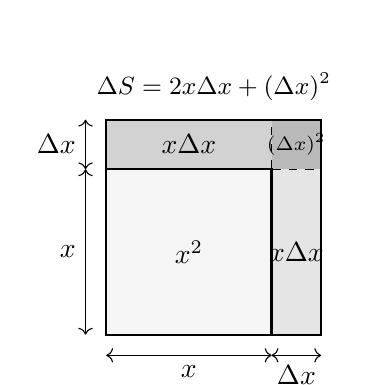
\begin{tikzpicture}[scale=1.05]
  \fill[gray!8] (0,0) rectangle (2,2);
  \fill[gray!20] (2,0) rectangle (2.6,2);
  \fill[gray!35] (0,2) rectangle (2,2.6);
  \fill[gray!55] (2,2) rectangle (2.6,2.6);
  \draw[thick] (0,0) rectangle (2,2);
  \draw[thick] (0,0) rectangle (2.6,2.6);
  \draw[dashed] (2,0)--(2,2.6);
  \draw[dashed] (0,2)--(2.6,2);
  \draw[<->] (0,-0.25)--(2,-0.25) node[midway,below] {$x$};
  \draw[<->] (2,-0.25)--(2.6,-0.25) node[midway,below] {$\Delta x$};
  \draw[<->] (-0.25,0)--(-0.25,2) node[midway,left] {$x$};
  \draw[<->] (-0.25,2)--(-0.25,2.6) node[midway,left] {$\Delta x$};
  \node at (1,1) {$x^2$};
  \node at (2.3,1) {$x\Delta x$};
  \node at (1,2.3) {$x\Delta x$};
  \node at (2.3,2.3) {\scriptsize $(\Delta x)^2$};
  \node at (1.3,3.0) {\small $\Delta S=2x\Delta x+(\Delta x)^2$};
\end{tikzpicture}
\end{center}

\begin{definition}[一元函数可微与微分]
设函数 $y=f(x)$ 在 $x$ 附近有定义。 当自变量增量为 $\Delta x$ 时，函数增量为
\[
\Delta y=f(x+\Delta x)-f(x).
\]
若存在与 $\Delta x$ 无关的常数 $A$，使得
\[
\Delta y=A\Delta x+o(\Delta x)\qquad(\Delta x\to0),
\]
则称 $f$ 在 $x$ 处可微，并称线性主部 $A\Delta x$ 为 $f$ 在 $x$ 处的微分，记作
\[
\dd y=A\Delta x.
\]
通常记 $\dd x=\Delta x$，于是微分写成 $\dd y=A\dd x$。
\end{definition}

\begin{theorem}[一元可导与可微等价]
$f$ 在 $x$ 处可微，当且仅当 $f$ 在 $x$ 处可导。 此时
\[
A=f'(x),\qquad \dd y=f'(x)\dd x.
\]
\end{theorem}
\begin{proofdetail}
若 $f$ 在 $x$ 处可微，则
\[
f(x+\Delta x)-f(x)=A\Delta x+o(\Delta x).
\]
当 $\Delta x\neq0$ 时，两边除以 $\Delta x$，得
\[
\frac{f(x+\Delta x)-f(x)}{\Delta x}
=A+\frac{o(\Delta x)}{\Delta x}.
\]
由 $o(\Delta x)$ 的定义，
\[
\frac{o(\Delta x)}{\Delta x}\to0\qquad(\Delta x\to0),
\]
所以导数存在，且 $f'(x)=A$。

反过来，若 $f$ 在 $x$ 处可导，则
\[
\frac{f(x+\Delta x)-f(x)}{\Delta x}\to f'(x).
\]
定义
\[
\alpha(\Delta x)=
\begin{cases}
\dfrac{f(x+\Delta x)-f(x)}{\Delta x}-f'(x),&\Delta x\neq0,\\[0.8em]
0,&\Delta x=0.
\end{cases}
\]
则 $\alpha(\Delta x)\to0$，并且
\[
\Delta y=f'(x)\Delta x+\alpha(\Delta x)\Delta x
=f'(x)\Delta x+o(\Delta x).
\]
因此 $f$ 在 $x$ 处可微，且 $\dd y=f'(x)\dd x$。
\end{proofdetail}

\begin{proposition}[微分运算法则]
若 $u=u(x),v=v(x)$ 在 $x$ 处可微，$c$ 为常数，则
\[
\dd(cu)=c\,\dd u,\qquad \dd(u+v)=\dd u+\dd v,
\]
\[
\dd(uv)=u\,\dd v+v\,\dd u,
\]
若 $v\neq0$，则
\[
\dd\left(\frac{u}{v}\right)=\frac{v\,\dd u-u\,\dd v}{v^2}.
\]
若 $y=f(u)$，$u=g(x)$，且相应函数可微，则
\[
\dd y=f'(u)\dd u.
\]
\end{proposition}
\begin{proofdetail}
由一元可导与可微等价，$u,v$ 可微等价于可导。 前四个公式分别由常数倍、和、积、商的求导法则乘以 $\dd x$ 得到。 例如
\[
\dd(uv)=(uv)'\dd x=(u'v+uv')\dd x=v(u'\dd x)+u(v'\dd x)=v\,\dd u+u\,\dd v.
\]
复合情形中，链式法则给出
\[
\dd y=\frac{\dd y}{\dd x}\dd x=f'(u)g'(x)\dd x=f'(u)\dd u.
\]
这说明无论 $u$ 是自变量还是 $x$ 的函数，微分形式 $\dd y=f'(u)\dd u$ 保持不变。
\end{proofdetail}

\begin{proposition}[微分的几何意义]
若 $f$ 在 $x_0$ 处可导，则曲线 $y=f(x)$ 在点 $M=(x_0,f(x_0))$ 附近可用切线作局部近似：
\[
f(x_0+\Delta x)-f(x_0)=f'(x_0)\Delta x+o(\Delta x).
\]
其中 $\Delta y=f(x_0+\Delta x)-f(x_0)$ 是真实增量，$\dd y=f'(x_0)\Delta x$ 是切线给出的线性近似，二者差为高阶误差。
\end{proposition}

\begin{center}
\begin{tikzpicture}[scale=1.0,>=Stealth]
  \draw[->] (-0.2,0)--(6.4,0) node[right] {$x$};
  \draw[->] (0,0.35)--(0,3.1) node[above] {$y$};
  \draw[domain=0.55:4.9,smooth,variable=\x,thick] plot ({\x},{0.16*(\x-1)*(\x-1)+1});
  \coordinate (M) at (2,1.16);
  \coordinate (T) at (3.4,1.608);
  \coordinate (N) at (3.4,1.922);
  \coordinate (B) at (3.4,1.16);
  \draw[thick] (0.7,0.744)--(5.15,2.168);
  \draw[dashed] (M)--(2,0) node[below] {$x_0$};
  \draw[dashed] (N)--(3.4,0) node[below] {$x_0+\Delta x$};
  \draw[dashed] (M)--(B);
  \draw[dashed] (N)--(T);
  \draw[dashed] (T)--(B);
  \draw[<->] (2,0.55)--(3.4,0.55) node[midway,below] {$\Delta x$};
  \draw[<->] (3.66,1.16)--(3.66,1.608);
  \draw[<->] (3.66,1.608)--(3.66,1.922);
  \draw[thin] (3.66,1.384)--(4.65,1.34) node[right] {$\dd y$};
  \draw[thin] (3.66,1.765)--(4.65,1.78) node[right] {\scriptsize $\Delta y-\dd y$};
  \fill (M) circle (1.5pt) node[above left] {$M$};
  \fill (T) circle (1.4pt) node[below left] {$T$};
  \fill (N) circle (1.5pt) node[above left] {$N$};
  \node[fill=white,inner sep=1pt] at (4.95,2.35) {切线};
\end{tikzpicture}
\end{center}

\begin{example}[近似计算]
用微分近似计算 $\sqrt{4.04}$。
\end{example}
\begin{solution}
取 $f(x)=\sqrt{x}$，在 $x=4$ 处线性化。 有
\[
f(4)=2,\qquad f'(x)=\frac{1}{2\sqrt{x}},\qquad f'(4)=\frac14.
\]
当 $\Delta x=0.04$ 时，
\[
\sqrt{4.04}=f(4+0.04)\approx f(4)+f'(4)\Delta x
=2+\frac14\cdot0.04=2.01.
\]
\end{solution}
\begin{warning}
微分近似不是等式。 本题真实值约为 $2.009975\cdots$，近似值 $2.01$ 的误差很小，是因为 $\Delta x=0.04$ 相对基点 $4$ 很小。
\end{warning}

\begin{example}[相对误差]
球的半径 $r$ 测量有小误差 $\Delta r$。 设体积 $V=\frac43\pi r^3$。 用微分估计体积的相对误差。
\end{example}
\begin{solution}
体积微分为
\[
\dd V=4\pi r^2\dd r.
\]
当 $\Delta r$ 很小时，$\Delta V\approx \dd V=4\pi r^2\Delta r$。 因此体积相对误差近似为
\[
\frac{\Delta V}{V}\approx
\frac{\dd V}{V}
=\frac{4\pi r^2\dd r}{\frac43\pi r^3}
=3\frac{\dd r}{r}.
\]
这说明半径的相对误差约放大为体积相对误差的三倍。 该结论来自数学模型 $V=\frac43\pi r^3$，不依赖具体计量单位。
\end{solution}

\begin{example}[微分形式不变性]
求函数
\[
y=\ee^{1-3x}\sin2x
\]
的微分。
\end{example}
\begin{solution}
由乘积微分法则，
\[
\dd y=\sin2x\,\dd(\ee^{1-3x})+\ee^{1-3x}\,\dd(\sin2x).
\]
利用微分形式不变性，
\[
\dd(\ee^{1-3x})=\ee^{1-3x}\dd(1-3x)=-3\ee^{1-3x}\dd x,
\]
\[
\dd(\sin2x)=\cos2x\,\dd(2x)=2\cos2x\,\dd x.
\]
故
\[
\dd y=\ee^{1-3x}(2\cos2x-3\sin2x)\dd x.
\]
\end{solution}



\subsection{偏导数与全微分}

	
	上一章讲述了二元函数的极限以及二元函数的连续性，描述函数在所有方向上的整体趋近行为；偏导数只考察平行于坐标轴的两个方向；可微性则要求函数增量能够由一个统一的线性表达式逼近。下面将依次学习偏导数与全微分，并进一步说明
	\[
	\text{可微}\Longrightarrow\text{连续},
	\]
	而偏导数存在一般不能推出连续。

\subsubsection*{偏导数}

二元函数 $z=f(x,y)$ 的输入是平面上的点。 若只让 $x$ 改变而保持 $y$ 不变，就得到沿平行于 $x$ 轴方向的变化率；若只让 $y$ 改变而保持 $x$ 不变，就得到沿平行于 $y$ 轴方向的变化率。 这两个变化率分别称为偏导数。

\begin{definition}[偏导数]
设 $z=f(x,y)$ 在点 $(x_0,y_0)$ 的某邻域内有定义。 若极限
\[
\lim_{h\to0}\frac{f(x_0+h,y_0)-f(x_0,y_0)}{h}
\]
存在，则称其为 $f$ 对 $x$ 的偏导数，记为
\[
f_x(x_0,y_0),\qquad \frac{\partial f}{\partial x}(x_0,y_0).
\]
若极限
\[
\lim_{k\to0}\frac{f(x_0,y_0+k)-f(x_0,y_0)}{k}
\]
存在，则称其为 $f$ 对 $y$ 的偏导数，记为 $f_y(x_0,y_0)$ 或 $\frac{\partial f}{\partial y}(x_0,y_0)$。
\end{definition}

\begin{example}[偏导计算]
设 $f(x,y)=x^2y+\sin(xy)$，求 $f_x,f_y$。
\end{example}
\begin{solution}
求 $f_x$ 时把 $y$ 看作常数：
\[
f_x=2xy+y\cos(xy).
\]
求 $f_y$ 时把 $x$ 看作常数：
\[
f_y=x^2+x\cos(xy).
\]
偏导计算中的“把另一个变量看作常数”不是说另一个变量永远不变，而是说此刻只沿一个坐标方向取变化率。
\end{solution}

\begin{example}[边际产量]
设 Cobb-Douglas 型生产函数为
\[
Q(K,L)=A K^\alpha L^\beta,\qquad A>0,\quad K>0,\quad L>0.
\]
其中 $K$ 表示资本投入，$L$ 表示劳动投入，$Q$ 表示产出。 求资本的边际产量和劳动的边际产量。
\end{example}
\begin{solution}
资本的边际产量指在劳动投入 $L$ 固定时，产出对资本投入 $K$ 的偏导数：
\[
Q_K=A\alpha K^{\alpha-1}L^\beta.
\]
劳动的边际产量指在资本投入 $K$ 固定时，产出对劳动投入 $L$ 的偏导数：
\[
Q_L=A\beta K^\alpha L^{\beta-1}.
\]
这两个量分别表示在当前投入水平附近，单独增加一单位资本或一单位劳动时，产出的近似增量。
\end{solution}

\begin{definition}[二阶偏导数]
若一阶偏导函数 $f_x,f_y$ 仍有偏导数，则称这些偏导数为二阶偏导数，记作
\[
f_{xx}=\frac{\partial^2 f}{\partial x^2},\qquad
f_{xy}=\frac{\partial^2 f}{\partial y\partial x},
\]
\[
f_{yx}=\frac{\partial^2 f}{\partial x\partial y},\qquad
f_{yy}=\frac{\partial^2 f}{\partial y^2}.
\]
这里 $f_{xy}$ 表示先对 $x$ 求偏导，再对 $y$ 求偏导；$f_{yx}$ 表示先对 $y$ 求偏导，再对 $x$ 求偏导。
\end{definition}

\begin{theorem}[混合偏导相等的充分条件]
若 $f_{xy}$ 与 $f_{yx}$ 在点 $(x_0,y_0)$ 的某邻域内存在，并且都在 $(x_0,y_0)$ 连续，则
\[
f_{xy}(x_0,y_0)=f_{yx}(x_0,y_0).
\]
\end{theorem}
\begin{proofdetail}
取充分小的非零 $h,k$，记
\[
\Delta=f(x_0+h,y_0+k)-f(x_0+h,y_0)-f(x_0,y_0+k)+f(x_0,y_0).
\]
先把 $\Delta$ 写为
\[
\Delta=\bigl[f(x_0+h,y_0+k)-f(x_0,y_0+k)\bigr]
-\bigl[f(x_0+h,y_0)-f(x_0,y_0)\bigr].
\]
对函数
\[
\Phi(y)=f(x_0+h,y)-f(x_0,y)
\]
在区间端点 $y_0,y_0+k$ 使用一元中值定理，存在 $\eta$ 介于 $0$ 与 $k$ 之间，使
\[
\Delta=\Phi'(y_0+\eta)k
=\bigl[f_y(x_0+h,y_0+\eta)-f_y(x_0,y_0+\eta)\bigr]k.
\]
再对函数 $x\mapsto f_y(x,y_0+\eta)$ 在 $x_0,x_0+h$ 上使用中值定理，存在 $\xi$ 介于 $0$ 与 $h$ 之间，使
\[
\Delta=f_{yx}(x_0+\xi,y_0+\eta)hk.
\]
因此
\[
\frac{\Delta}{hk}=f_{yx}(x_0+\xi,y_0+\eta).
\]

另一方面，把 $\Delta$ 写为
\[
\Delta=\bigl[f(x_0+h,y_0+k)-f(x_0+h,y_0)\bigr]
-\bigl[f(x_0,y_0+k)-f(x_0,y_0)\bigr],
\]
同理可得存在 $\xi_1$ 介于 $0$ 与 $h$ 之间、$\eta_1$ 介于 $0$ 与 $k$ 之间，使
\[
\frac{\Delta}{hk}=f_{xy}(x_0+\xi_1,y_0+\eta_1).
\]
令 $(h,k)\to(0,0)$，由 $f_{xy},f_{yx}$ 在 $(x_0,y_0)$ 连续，两种表示的极限分别为 $f_{xy}(x_0,y_0)$ 与 $f_{yx}(x_0,y_0)$，而左端是同一个量的极限，故两者相等。
\end{proofdetail}

\begin{example}[二阶偏导]
设 $f(x,y)=x^3y^2+\ee^{xy}$，求 $f_{xy}$ 与 $f_{yx}$。
\end{example}
\begin{solution}
先求
\[
f_x=3x^2y^2+y\ee^{xy},
\]
再对 $y$ 求偏导：
\[
f_{xy}=6x^2y+\ee^{xy}+xy\ee^{xy}.
\]
另一方面，
\[
f_y=2x^3y+x\ee^{xy},
\]
再对 $x$ 求偏导：
\[
f_{yx}=6x^2y+\ee^{xy}+xy\ee^{xy}.
\]
两者相等。 这里函数由初等函数复合而成，各相关偏导连续，因此符合混合偏导相等的充分条件。
\end{solution}

\begin{example}[偏导存在不推出连续]
设
\[
f(x,y)=
\begin{cases}
\dfrac{xy}{x^2+y^2},&(x,y)\neq(0,0),\\[0.6em]
0,&(x,y)=(0,0).
\end{cases}
\]
证明 $f_x(0,0),f_y(0,0)$ 存在，但 $f$ 在 $(0,0)$ 不连续。
\end{example}
\begin{solution}
按定义，
\[
f_x(0,0)=\lim_{h\to0}\frac{f(h,0)-f(0,0)}{h}=0,\qquad
f_y(0,0)=\lim_{h\to0}\frac{f(0,h)-f(0,0)}{h}=0.
\]
但沿直线 $y=x$，
\[
f(x,x)=\frac{x^2}{2x^2}=\frac12\quad(x\neq0),
\]
故 $\lim_{(x,y)\to(0,0)}f(x,y)$ 不等于 $0$，函数在原点不连续。
\end{solution}
\begin{warning}
偏导数只检测坐标轴方向的变化，不能控制所有趋近方向。因此“两个偏导数都存在”远弱于“二元函数可微”，也不能保证函数连续。
\end{warning}

\subsubsection*{隐函数求导}

前面讨论的函数大多写成 $y=f(x)$，这种形式称为显函数。 但在实际问题和几何问题中，变量之间常由方程给出，例如
\[
x^2+y^2=1,\qquad x^2+xy+y^2=3.
\]
它们未必能方便地解出 $y=f(x)$。 由方程 $F(x,y)=0$ 在某个范围内确定的函数称为隐函数。 例如
\[
\sqrt{y}+x^2-1=0
\]
在满足 $1-x^2\geq0$ 且 $\sqrt{y}=1-x^2$ 的范围内可写成
\[
y=(1-x^2)^2.
\]
但并不是每个方程都在任意点附近确定唯一函数。 本讲义在求导时默认题目所给方程已经在所讨论点附近确定了可导函数；更一般的存在唯一性条件将在多元函数课程中进一步解释。

\begin{center}
	\begin{tikzpicture}[scale=1.15,>=Stealth]
		\draw[->] (-1.9,0) -- (1.9,0) node[right] {$x$};
		\draw[->] (0,-1.55) -- (0,1.55) node[above] {$y$};
		\draw[thick,domain=0:360,samples=160] plot ({cos(\x)},{sin(\x)});
		\fill (0.6,0.8) circle (1.5pt) node[above right] {$P(x,y)$};
		\draw[dashed] (0.6,0) -- (0.6,0.8) -- (0,0.8);
		\node at (0,-1.85) {$x^2+y^2=1$ 给出的曲线可在局部看作 $y=y(x)$};
	\end{tikzpicture}
\end{center}

\begin{proposition}[隐函数一阶求导]
	若方程 $F(x,y)=0$ 在某区间上确定可导函数 $y=y(x)$，且 $F$ 有连续偏导数、$F_y(x,y)\neq0$，则
	\[
	y'=-\frac{F_x}{F_y},
	\]
	其中右端在 $(x,y(x))$ 处取值。
\end{proposition}
\begin{proofdetail}
	由恒等式 $F(x,y(x))\equiv0$ 对 $x$ 求导。 复合函数求导给出
	\[
	F_x(x,y(x))+F_y(x,y(x))y'(x)=0.
	\]
	由于 $F_y(x,y(x))\neq0$，移项并相除得到公式。
\end{proofdetail}

\begin{example}[隐函数一阶导数]
	由方程 $x^2+xy+y^2=3$ 确定 $y=y(x)$，求 $y'$。
\end{example}
\begin{solution}
	两边对 $x$ 求导：
	\[
	2x+y+xy'+2yy'=0.
	\]
	整理得
	\[
	y'=-\frac{2x+y}{x+2y}.
	\]
	该公式在 $x+2y\neq0$ 的点成立。
\end{solution}

\begin{example}[先说明隐函数再求导]
	设方程
	\[
	\sqrt{y}+x^2-1=0
	\]
	在 $|x|<1$ 附近确定函数 $y=y(x)$。 用两种方法求 $y'$。
\end{example}
\begin{solution}
	方法一：先解出显函数。 由方程得
	\[
	\sqrt{y}=1-x^2.
	\]
	当 $|x|<1$ 时右端为正，故
	\[
	y=(1-x^2)^2.
	\]
	于是
	\[
	y'=2(1-x^2)(-2x)=-4x(1-x^2).
	\]
	
	方法二：直接对原方程求导。 注意
	\[
	\frac{\dd}{\dd x}\sqrt{y}
	=\frac{1}{2\sqrt{y}}y',
	\]
	因此
	\[
	\frac{y'}{2\sqrt{y}}+2x=0,
	\qquad
	y'=-4x\sqrt{y}.
	\]
	再代入 $\sqrt{y}=1-x^2$，得
	\[
	y'=-4x(1-x^2).
	\]
	两种方法结果一致。
\end{solution}

\begin{example}[隐函数二阶导数]
	设 $x^2+y^2=1$ 在点附近确定 $y=y(x)$，求 $y''$。
\end{example}
\begin{solution}
	一阶求导得
	\[
	2x+2yy'=0,\qquad y'=-\frac{x}{y}\quad(y\neq0).
	\]
	对 $2x+2yy'=0$ 再求导：
	\[
	2+2(y')^2+2yy''=0.
	\]
	故
	\[
	y''=-\frac{1+(y')^2}{y}=-\frac{1+x^2/y^2}{y}
	=-\frac{x^2+y^2}{y^3}=-\frac1{y^3}.
	\]
\end{solution}

\begin{example}[隐函数切线]
	求曲线
	\[
	xy-\ee^x+\ee^y=0
	\]
	在点 $(0,0)$ 处的切线方程。
\end{example}
\begin{solution}
	把 $y$ 看成 $x$ 的函数，对方程两边求导，得
	\[
	y+xy'-\ee^x+\ee^y y'=0.
	\]
	整理得
	\[
	(x+\ee^y)y'=\ee^x-y,\qquad
	y'=\frac{\ee^x-y}{x+\ee^y}.
	\]
	在 $(0,0)$ 处，
	\[
	y'(0)=\frac{1-0}{0+1}=1.
	\]
	因此切线方程为 $y=x$。
\end{solution}



\subsubsection*{全微分与多元链式法则}

二元函数的偏导数只给出两个坐标方向的变化率。 若要像一元函数那样用一个线性表达式近似总增量，就需要全微分。 全微分的线性主部同时包含 $\Delta x$ 与 $\Delta y$：
\[
\Delta z\approx f_x(x_0,y_0)\Delta x+f_y(x_0,y_0)\Delta y.
\]

\begin{definition}[二元函数可微与全微分]
设 $z=f(x,y)$ 在 $(x_0,y_0)$ 附近有定义。 若
\[
\Delta z=f(x_0+\Delta x,y_0+\Delta y)-f(x_0,y_0)
\]
可写成
\[
\Delta z=A\Delta x+B\Delta y+o(\rho),
\qquad \rho=\sqrt{(\Delta x)^2+(\Delta y)^2},
\]
则称 $f$ 在 $(x_0,y_0)$ 可微，并称
\[
\dd z=A\dd x+B\dd y
\]
为 $f$ 在该点的全微分。
\end{definition}

\begin{theorem}[可微推出连续且偏导存在]
若 $f$ 在 $(x_0,y_0)$ 可微，则 $f$ 在该点连续，且 $f_x(x_0,y_0),f_y(x_0,y_0)$ 存在，并且
\[
\dd z=f_x(x_0,y_0)\dd x+f_y(x_0,y_0)\dd y.
\]
\end{theorem}
\begin{proofdetail}
由可微性，
\[
\Delta z=A\Delta x+B\Delta y+o(\rho).
\]
由于 $|\Delta x|\leq\rho,\ |\Delta y|\leq\rho$，当 $\rho\to0$ 时，
\[
A\Delta x+B\Delta y\to0,\qquad o(\rho)\to0.
\]
故 $\Delta z\to0$，即 $f$ 在 $(x_0,y_0)$ 连续。

取 $\Delta y=0$，则 $\rho=|\Delta x|$，且
\[
f(x_0+\Delta x,y_0)-f(x_0,y_0)=A\Delta x+o(|\Delta x|).
\]
当 $\Delta x\neq0$ 时除以 $\Delta x$ 并令 $\Delta x\to0$，得
\[
f_x(x_0,y_0)=A.
\]
同理取 $\Delta x=0$ 得 $f_y(x_0,y_0)=B$。 因此
\[
\dd z=f_x(x_0,y_0)\dd x+f_y(x_0,y_0)\dd y.
\]
\end{proofdetail}

\begin{theorem}[偏导连续推出可微]
若 $f_x,f_y$ 在 $(x_0,y_0)$ 的某邻域内存在，并且在 $(x_0,y_0)$ 连续，则 $f$ 在 $(x_0,y_0)$ 可微。
\end{theorem}
\begin{proofdetail}
记
\[
\Delta z=f(x_0+\Delta x,y_0+\Delta y)-f(x_0,y_0).
\]
分两段改变变量：
\[
\Delta z=[f(x_0+\Delta x,y_0+\Delta y)-f(x_0,y_0+\Delta y)]
+[f(x_0,y_0+\Delta y)-f(x_0,y_0)].
\]
对第一项把 $y_0+\Delta y$ 固定，对一元函数 $x\mapsto f(x,y_0+\Delta y)$ 使用中值定理。 当 $\Delta x\neq0$ 时，存在 $\theta_1\in(0,1)$ 使
\[
f(x_0+\Delta x,y_0+\Delta y)-f(x_0,y_0+\Delta y)
=f_x(x_0+\theta_1\Delta x,y_0+\Delta y)\Delta x.
\]
当 $\Delta x=0$ 时该等式也成立，因为两边均为 $0$，$\theta_1$ 可任取。 对第二项同理，存在 $\theta_2\in(0,1)$ 使
\[
f(x_0,y_0+\Delta y)-f(x_0,y_0)
=f_y(x_0,y_0+\theta_2\Delta y)\Delta y.
\]
于是
\[
\Delta z=f_x(x_0,y_0)\Delta x+f_y(x_0,y_0)\Delta y+R,
\]
其中
\[
R=[f_x(x_0+\theta_1\Delta x,y_0+\Delta y)-f_x(x_0,y_0)]\Delta x
\]
\[
\quad+[f_y(x_0,y_0+\theta_2\Delta y)-f_y(x_0,y_0)]\Delta y.
\]
由 $f_x,f_y$ 在 $(x_0,y_0)$ 连续，两个方括号中的差都趋于 $0$。 又 $|\Delta x|\leq\rho,\ |\Delta y|\leq\rho$，所以 $R=o(\rho)$。 因此 $f$ 可微。
\end{proofdetail}

\begin{center}
\begin{tikzpicture}[scale=1.0,>=Stealth]
  \draw[->] (-0.2,0)--(5.2,0) node[right] {$x$};
  \draw[->] (0,-0.2)--(0,3.4) node[above] {$y$};
  \coordinate (P) at (1.3,1.0);
  \coordinate (A) at (4.2,1.0);
  \coordinate (B) at (4.2,2.75);
  \coordinate (C) at (1.3,2.75);
  \draw[dashed] (P)--(A)--(B);
  \draw[dashed] (P)--(C)--(B);
  \draw[->,thick] (P)--(A) node[midway,below] {$\Delta x$};
  \draw[->,thick] (A)--(B) node[midway,right] {$\Delta y$};
  \draw[->,thick] (P)--(C) node[midway,left] {$\Delta y$};
  \draw[->,thick] (C)--(B) node[midway,above] {$\Delta x$};
  \fill (P) circle (1.5pt) node[below left] {$(x_0,y_0)$};
  \fill (B) circle (1.5pt) node[right=3pt] {$(x_0+\Delta x,y_0+\Delta y)$};
  \node at (2.75,3.55) {\small 总增量可沿两段坐标方向分解};
\end{tikzpicture}
\end{center}

\begin{example}[全微分近似]
估计 $f(x,y)=x^2y+\ln y$ 在 $(2,1)$ 附近，当 $x$ 增加 $0.01$、$y$ 减少 $0.02$ 时的函数增量。
\end{example}
\begin{solution}
\[
f_x=2xy,\qquad f_y=x^2+\frac1y.
\]
在 $(2,1)$ 处，
\[
f_x(2,1)=4,\qquad f_y(2,1)=5.
\]
故
\[
\Delta f\approx \dd f=4(0.01)+5(-0.02)=0.04-0.10=-0.06.
\]
这里的 $-0.06$ 是函数真实增量的线性近似；若要得到真实增量，需要代入原函数计算。
\end{solution}

\begin{example}[可微性判断]
证明函数
\[
f(x,y)=x^2+y^2+xy
\]
在任意点可微，并求其全微分。
\end{example}
\begin{solution}
先求偏导数：
\[
f_x=2x+y,\qquad f_y=2y+x.
\]
这两个偏导函数在全平面连续。 由偏导连续推出可微的定理，$f$ 在任意点可微，且
\[
\dd z=(2x+y)\dd x+(2y+x)\dd y.
\]
\end{solution}

\begin{theorem}[二元链式法则：一元参数情形]
设 $z=f(x,y)$ 在点 $(x(t),y(t))$ 处可微，且 $x=x(t),y=y(t)$ 在 $t$ 处可导，则复合函数 $z=f(x(t),y(t))$ 在 $t$ 处可导，且
\[
\frac{\dd z}{\dd t}=f_x\frac{\dd x}{\dd t}+f_y\frac{\dd y}{\dd t},
\]
其中 $f_x,f_y$ 在点 $(x(t),y(t))$ 处取值。
\end{theorem}
\begin{proofdetail}
由 $f$ 可微，
\[
\Delta z=f_x\Delta x+f_y\Delta y+o(\rho),
\qquad \rho=\sqrt{(\Delta x)^2+(\Delta y)^2}.
\]
两边除以 $\Delta t$。 因 $x,y$ 在 $t$ 处可导，故
\[
\Delta x=x'(t)\Delta t+o(\Delta t),\qquad
\Delta y=y'(t)\Delta t+o(\Delta t).
\]
于是 $\rho=O(|\Delta t|)$。 因此
\[
\frac{o(\rho)}{\Delta t}
=\frac{o(\rho)}{\rho}\cdot\frac{\rho}{\Delta t}\to0,
\]
其中第二个因子有界。 令 $\Delta t\to0$，得到
\[
\frac{\dd z}{\dd t}=f_x x'(t)+f_y y'(t).
\]
\end{proofdetail}

\begin{center}
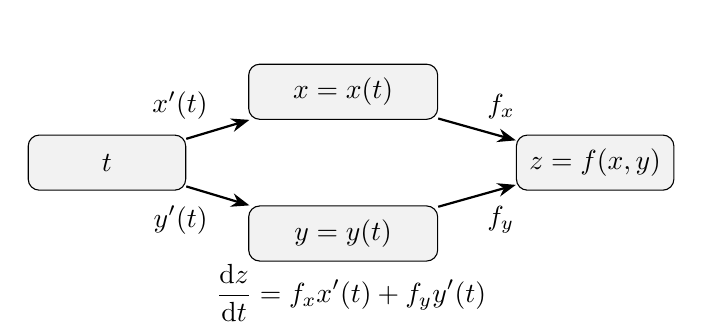
\begin{tikzpicture}[>=Stealth,scale=1.0]
  \node[draw,rounded corners,fill=gray!10,minimum width=2cm,minimum height=0.7cm] (t) at (0,0) {$t$};
  \node[draw,rounded corners,fill=gray!10,minimum width=2.4cm,minimum height=0.7cm] (x) at (3,0.9) {$x=x(t)$};
  \node[draw,rounded corners,fill=gray!10,minimum width=2.4cm,minimum height=0.7cm] (y) at (3,-0.9) {$y=y(t)$};
  \node[draw,rounded corners,fill=gray!10,minimum width=2cm,minimum height=0.7cm] (z) at (6.2,0) {$z=f(x,y)$};
  \draw[->,thick] (t)--(x) node[midway,above left] {$x'(t)$};
  \draw[->,thick] (t)--(y) node[midway,below left] {$y'(t)$};
  \draw[->,thick] (x)--(z) node[midway,above right] {$f_x$};
  \draw[->,thick] (y)--(z) node[midway,below right] {$f_y$};
  \node at (3.1,-1.65) {$\displaystyle \frac{\dd z}{\dd t}=f_xx'(t)+f_yy'(t)$};
\end{tikzpicture}
\end{center}

\begin{example}[多元链式法则]
设
\[
z=x^2y+\sin y,\qquad x=t^2,\qquad y=\ee^t.
\]
求 $\frac{\dd z}{\dd t}$。
\end{example}
\begin{solution}
先求
\[
z_x=2xy,\qquad z_y=x^2+\cos y.
\]
又
\[
\frac{\dd x}{\dd t}=2t,\qquad \frac{\dd y}{\dd t}=\ee^t.
\]
由链式法则，
\[
\frac{\dd z}{\dd t}
=z_x\frac{\dd x}{\dd t}+z_y\frac{\dd y}{\dd t}
=2xy\cdot2t+(x^2+\cos y)\ee^t.
\]
代入 $x=t^2,\ y=\ee^t$，得
\[
\frac{\dd z}{\dd t}
=4t^3\ee^t+(t^4+\cos(\ee^t))\ee^t.
\]
\end{solution}

\begin{theorem}[二元链式法则：二元中间变量情形]
设 $z=f(u,v)$ 在相应点可微，且
\[
u=u(x,y),\qquad v=v(x,y)
\]
在 $(x,y)$ 处有连续偏导数，则复合函数 $z=f(u(x,y),v(x,y))$ 在该点的偏导数为
\[
\frac{\partial z}{\partial x}=f_u\frac{\partial u}{\partial x}+f_v\frac{\partial v}{\partial x},
\qquad
\frac{\partial z}{\partial y}=f_u\frac{\partial u}{\partial y}+f_v\frac{\partial v}{\partial y}.
\]
\end{theorem}
\begin{proofdetail}
只证关于 $x$ 的公式，关于 $y$ 的公式同理。 固定 $y$，令 $x$ 改变为 $x+\Delta x$。 由于 $u,v$ 对 $x$ 可导，
\[
\Delta u=u_x\Delta x+o(\Delta x),\qquad
\Delta v=v_x\Delta x+o(\Delta x).
\]
由 $f$ 在 $(u,v)$ 处可微，
\[
\Delta z=f_u\Delta u+f_v\Delta v+o(\rho),
\qquad \rho=\sqrt{(\Delta u)^2+(\Delta v)^2}.
\]
又 $\Delta u=O(\Delta x),\Delta v=O(\Delta x)$，故 $\rho=O(|\Delta x|)$，从而 $o(\rho)=o(\Delta x)$。 代入得
\[
\Delta z=(f_u u_x+f_v v_x)\Delta x+o(\Delta x).
\]
两边除以 $\Delta x$ 并令 $\Delta x\to0$，得到
\[
\frac{\partial z}{\partial x}=f_u u_x+f_v v_x.
\]
\end{proofdetail}

\begin{example}[二元复合函数偏导]
设 $z=f(x^2+y,xy)$，其中 $f$ 有连续一阶偏导数。 求 $\frac{\partial z}{\partial x}$ 与 $\frac{\partial z}{\partial y}$。
\end{example}
\begin{solution}
令
\[
u=x^2+y,\qquad v=xy.
\]
则 $z=f(u,v)$。 记 $f_u,f_v$ 分别为 $f$ 对第一、第二个变量的偏导数，并在 $(u,v)=(x^2+y,xy)$ 处取值。 由链式法则，
\[
\frac{\partial z}{\partial x}
=f_u\frac{\partial u}{\partial x}+f_v\frac{\partial v}{\partial x}
=2x f_u+y f_v,
\]
\[
\frac{\partial z}{\partial y}
=f_u\frac{\partial u}{\partial y}+f_v\frac{\partial v}{\partial y}
=f_u+x f_v.
\]
\end{solution}



\begin{application}[作物产量对水分和氮肥的敏感性]
设简化产量模型为
\[
Y=Y(W,N),
\]
其中 $W$ 是灌溉量（$\mathrm{m^3/ha}$），$N$ 是氮肥投入量（$\mathrm{kg/ha}$），$Y$ 是产量（$\mathrm{t/ha}$）。在其他条件暂时保持不变的局部分析中，
\[
\frac{\partial Y}{\partial W}
\]
表示施肥条件不变时，灌溉量微小改变对产量的局部影响；而
\[
\frac{\partial Y}{\partial N}
\]
表示水分条件不变时，氮肥投入微小改变的局部影响。若 $Y$ 可微，且 $\Delta W,\Delta N$ 较小，则
\[
\Delta Y\approx Y_W\Delta W+Y_N\Delta N.
\]
这正体现了偏导数与全微分的区别。真实产量还受温度、土壤、品种、病虫害以及水肥交互作用影响，因此该局部模型不能直接给出灌溉或施肥处方。\upcite{TaizPlant}
\end{application}


\begin{application}[偏导数在多参数机器学习模型中的应用]
	
	多元函数的偏导数可以直接解释多参数模型训练。 设有 $m$ 个样本 $(x_i,y_i)$，用一元线性模型
	\[
	\hat y_i=wx_i+b
	\]
	进行预测。 常用的均方误差损失为
	\[
	J(w,b)=\frac{1}{2m}\sum_{i=1}^{m}(wx_i+b-y_i)^2.
	\]
	这里 $J$ 是关于两个变量 $w,b$ 的函数。 对 $w$ 和 $b$ 分别求偏导，得
	\[
	\frac{\partial J}{\partial w}
	=\frac{1}{m}\sum_{i=1}^{m}(wx_i+b-y_i)x_i,
	\qquad
	\frac{\partial J}{\partial b}
	=\frac{1}{m}\sum_{i=1}^{m}(wx_i+b-y_i).
	\]
	梯度下降更新为
	\[
	w_{k+1}=w_k-\eta\frac{\partial J}{\partial w}(w_k,b_k),\qquad
	b_{k+1}=b_k-\eta\frac{\partial J}{\partial b}(w_k,b_k).
	\]
	
	\begin{example}
		对两个样本 $(1,2),(2,3)$，写出线性模型 $\hat y=wx+b$ 的损失函数，并求 $\nabla J(0,0)$。
	\end{example}
	\begin{solution}
		此时 $m=2$，
		\[
		J(w,b)=\frac14\left[(w+b-2)^2+(2w+b-3)^2\right].
		\]
		由上面的公式，
		\[
		\frac{\partial J}{\partial w}
		=\frac12\left[(w+b-2)\cdot1+(2w+b-3)\cdot2\right],
		\]
		\[
		\frac{\partial J}{\partial b}
		=\frac12\left[(w+b-2)+(2w+b-3)\right].
		\]
		代入 $(w,b)=(0,0)$，
		\[
		\frac{\partial J}{\partial w}(0,0)=\frac12[-2+2(-3)]=-4,\qquad
		\frac{\partial J}{\partial b}(0,0)=\frac12(-2-3)=-\frac52.
		\]
		故
		\[
		\nabla J(0,0)=\left(-4,-\frac52\right).
		\]
		若学习率为 $\eta$，第一次更新为
		\[
		(w_1,b_1)=\left(0,0\right)-\eta\left(-4,-\frac52\right)
		=\left(4\eta,\frac52\eta\right).
		\]
	\end{solution}
	
	
	
	
\end{application}





\iffalse

\subsection*{第5章课后习题}
\addcontentsline{toc}{subsection}{第5章课后习题}

\subsubsection*{第5.1--5.3节\quad 导数的概念与意义}

\begin{enumerate}[label=\textbf{练习\arabic*.},leftmargin=2.2em]
\item 判断下列函数在指定点是否可导：
\[
|x-1|\text{ 在 }x=1;\qquad
x^{2/3}\text{ 在 }x=0;\qquad
\begin{cases}x\sin\frac1x,&x\neq0,\\0,&x=0,\end{cases}\text{ 在 }x=0.
\]
\item 求曲线 $y=x^2-2x$ 在点 $(1,-1)$ 处的切线方程和法线方程。
\item 设总成本函数 $C(x)=0.02x^2+8x+500$，求边际成本函数，并解释 $C'(100)$ 的含义。
\item 用导数定义求 $f(x)=\frac1x$ 在 $x_0\neq0$ 处的导数。
\item 设需求函数 $x=80-2p$。 求收入函数 $R(x)$ 与边际收入函数，并求 $x=30$ 时的边际收入。
\item 设
\[
f(x)=
\begin{cases}
ax+b,&x<1,\\
x^2,&x\geq1.
\end{cases}
\]
求 $a,b$，使 $f$ 在 $x=1$ 处可导。
\end{enumerate}

\subsubsection*{第5.4--5.6节\quad 一元函数求导法则}

\begin{enumerate}[label=\textbf{练习\arabic*.},leftmargin=2.2em]
\item 求下列函数的导数：
\[
y=3x^2+4\ln x-5\cos x,\qquad
y=\ln(\sin x),\qquad
y=\ee^{\sqrt{x}}.
\]
\item 求
\[
y=\frac{x^2\sin x}{1+x^2}
\]
的导数，并说明用到了哪些求导法则。
\item 求下列函数的导数：
\[
y=(1+x^2)^{\arctan x},\qquad
y=(\cot x)^{\cos x}.
\]
\item 由反函数求导公式推出 $y=\arccos x$ 的导数。
\item 求 $y=x^2\ln x$ 的二阶导数，其中 $x>0$。
\item 求 $y=x^2\ee^x$ 的 $n$ 阶导数。
\item 设 $x^3+y^3-3xy=0$ 确定 $y=y(x)$，求 $y'$。
\item 求曲线
\[
xy+\ln y=1
\]
在点 $(1,1)$ 处的切线方程。
\item 曲线由参数方程
\[
x=t-\sin t,\qquad y=1-\cos t
\]
给出，求 $\frac{\dd y}{\dd x}$。
\item 某产品总收入函数为
\[
R(x)=50x-0.1x^2.
\]
求边际收入函数和边际收入的变化率，并解释 $R''(x)$ 的经济含义。
\end{enumerate}

\subsubsection*{第5.7--5.11节\quad 微分、偏导数与多元微分}

\begin{enumerate}[label=\textbf{练习\arabic*.},leftmargin=2.2em]
\item 判断下列命题真伪，并说明理由：偏导数存在必连续；连续且偏导存在必可微；偏导数连续必可微；可微必连续。
\item 求 $z=x^2y+\ee^{xy}$ 的全微分。
\item 用微分近似计算 $\sqrt{9.06}$。
\item 用微分估计 $\ln(1.02)$。
\item 设 $f(x,y)=x^3y^2+\ee^{xy}$，求 $f_x,f_y,f_{xy},f_{yx}$。
\item 设生产函数 $Q(K,L)=10K^{1/2}L^{1/2}$。 求 $Q_K,Q_L$，并解释它们的意义。
\item 证明函数 $f(x,y)=x^2+y^2-2xy$ 在任意点可微，并写出全微分。
\item 设 $z=x^2y+\sin y,\ x=t^2,\ y=\ee^t$。 求 $\frac{\dd z}{\dd t}$。
\item 设 $z=f(x^2+y,xy)$，其中 $f$ 有连续一阶偏导数。 求 $\frac{\partial z}{\partial x}$ 与 $\frac{\partial z}{\partial y}$。
\item 设
\[
f(x,y)=
\begin{cases}
\dfrac{x^2y}{x^2+y^2},&(x,y)\neq(0,0),\\[0.6em]
0,&(x,y)=(0,0).
\end{cases}
\]
求 $f_x(0,0),f_y(0,0)$，并判断 $f$ 在 $(0,0)$ 是否连续。
\end{enumerate}

\subsection*{第5章参考答案与提示}
\addcontentsline{toc}{subsection}{第5章参考答案与提示}

\subsubsection*{第5.1--5.3节\quad 导数的概念与意义}

\begin{enumerate}[label=\textbf{练习\arabic*.},leftmargin=2.2em]
\item $|x-1|$ 在 $x=1$ 左导数为 $-1$，右导数为 $1$，不可导；$x^{2/3}$ 在 $0$ 处差商为 $h^{-1/3}$，极限不存在，作为有限导数不可导；第三个函数在 $0$ 处差商为 $\sin(1/h)$，极限不存在，故不可导。
\item $y'=2x-2$，在 $x=1$ 处斜率为 $0$。 切线为 $y=-1$，法线为 $x=1$。
\item $C'(x)=0.04x+8$，故 $C'(100)=12$。 它表示产量在 $100$ 附近增加一个单位时，总成本约增加 $12$ 个成本单位。
\item
\[
\frac{f(x_0+h)-f(x_0)}{h}
=\frac{\frac1{x_0+h}-\frac1{x_0}}{h}
=-\frac1{x_0(x_0+h)}.
\]
令 $h\to0$，得 $f'(x_0)=-\frac1{x_0^2}$。
\item 由 $x=80-2p$ 得 $p=40-\frac{x}{2}$。 因此
\[
R(x)=xp=40x-\frac{x^2}{2},\qquad R'(x)=40-x.
\]
故 $R'(30)=10$，表示销量为 $30$ 附近多销售一个单位时，总收入约增加 $10$。
\item 可导必连续，先由连续性得
\[
a+b=1.
\]
左导数为 $a$，右导数为 $2$，可导要求 $a=2$。 代回得 $b=-1$。
\end{enumerate}

上一章给出了导数的定义。 如果每遇到一个函数都从差商
\[
\frac{f(x+h)-f(x)}{h}
\]
出发求极限，理论上可行，但实际计算会非常繁琐。 本章的任务是把“从定义求导”的工作整理成一套可靠的计算规则：简单函数用基本公式，复杂函数先分解结构，再按线性组合、乘积、商、复合、反函数、隐函数或参数方程分别处理。

求导法则不是独立于导数定义之外的技巧，而是由极限运算法则和可导函数的连续性推出的。 因此使用公式时必须同时注意两个问题：第一，函数在所讨论的点是否有定义；第二，公式中的分母、根式、反函数条件等是否允许这样求导。

\subsubsection*{第5.4--5.6节\quad 一元函数求导法则}

\begin{enumerate}[label=\textbf{练习\arabic*.},leftmargin=2.2em]
\item
\[
(3x^2+4\ln x-5\cos x)'=6x+\frac4x+5\sin x.
\]
又
\[
(\ln\sin x)'=\frac{\cos x}{\sin x}=\cot x,
\]
其中需 $\sin x>0$ 或至少在选定区间内 $\ln(\sin x)$ 有定义。 最后
\[
(\ee^{\sqrt{x}})'=\ee^{\sqrt{x}}\cdot\frac1{2\sqrt{x}}
=\frac{\ee^{\sqrt{x}}}{2\sqrt{x}},\qquad x>0.
\]
\item 先对分子用乘积法则，再对整体用商法：
\[
\left(x^2\sin x\right)'=2x\sin x+x^2\cos x,
\]
\[
y'=\frac{(2x\sin x+x^2\cos x)(1+x^2)-2x\cdot x^2\sin x}{(1+x^2)^2}.
\]
化简得
\[
y'=\frac{2x\sin x+x^2\cos x+x^4\cos x}{(1+x^2)^2}.
\]
\item 对第一个函数取对数：
\[
\ln y=(\arctan x)\ln(1+x^2),
\]
故
\[
y'=(1+x^2)^{\arctan x}\left[\frac{\ln(1+x^2)}{1+x^2}+\frac{2x\arctan x}{1+x^2}\right].
\]
对第二个函数，取对数得
\[
\ln y=\cos x\ln(\cot x).
\]
因此
\[
y'=(\cot x)^{\cos x}\left[-\sin x\ln(\cot x)-\frac1{\sin x}\right],
\]
其中要求在所讨论区间内 $\cot x>0$。
\item 令 $y=\arccos x$，则 $x=\cos y$，$y\in[0,\pi]$。 当 $-1<x<1$ 时，$\sin y>0$，故
\[
\frac{\dd x}{\dd y}=-\sin y=-\sqrt{1-x^2}.
\]
由反函数求导公式，
\[
(\arccos x)'=-\frac1{\sqrt{1-x^2}},\qquad -1<x<1.
\]
\item
\[
y'=2x\ln x+x,\qquad y''=2\ln x+3.
\]
\item 由莱布尼茨公式，取 $u=x^2,\ v=\ee^x$。 因 $u^{(k)}=0\ (k\geq3)$，得
\[
y^{(n)}=\ee^x\left[x^2+2nx+n(n-1)\right].
\]
\item 两边对 $x$ 求导：
\[
3x^2+3y^2y'-3y-3xy'=0,
\]
故
\[
y'=\frac{y-x^2}{y^2-x}.
\]
\item 将 $y$ 看成 $x$ 的函数。 对
\[
xy+\ln y=1
\]
两边求导：
\[
y+xy'+\frac{y'}{y}=0.
\]
在 $(1,1)$ 处，
\[
1+y'+y'=0,\qquad y'=-\frac12.
\]
故切线方程为
\[
y-1=-\frac12(x-1).
\]
\item
\[
\frac{\dd y}{\dd x}=\frac{\sin t}{1-\cos t},
\]
其中 $1-\cos t\neq0$。
\item
\[
R'(x)=50-0.2x,\qquad R''(x)=-0.2.
\]
其中 $R'(x)$ 为边际收入，表示销量在 $x$ 附近增加一个单位时收入的近似增量；$R''(x)=-0.2$ 表示边际收入随销量增加而下降，且下降速度为常数 $0.2$。
\end{enumerate}

\subsubsection*{第5.7--5.11节\quad 微分、偏导数与多元微分}

\begin{enumerate}[label=\textbf{练习\arabic*.},leftmargin=2.2em]
\item 偏导数存在不一定连续，反例可取本章例题
\[
f(x,y)=\frac{xy}{x^2+y^2},\quad f(0,0)=0.
\]
连续且偏导存在不一定可微；例如
\[
f(x,y)=
\begin{cases}
\dfrac{xy}{\sqrt{x^2+y^2}},&(x,y)\neq(0,0),\\[0.6em]
0,&(x,y)=(0,0).
\end{cases}
\]
在原点连续，且
\[
f_x(0,0)=\lim_{h\to0}\frac{f(h,0)-0}{h}=0,\qquad
f_y(0,0)=\lim_{k\to0}\frac{f(0,k)-0}{k}=0.
\]
若它在原点可微，则线性主部应为 $0\cdot x+0\cdot y=0$。 但沿 $y=x$，
\[
\frac{f(x,x)-0}{\sqrt{x^2+x^2}}
=\frac{x^2/\sqrt{2x^2}}{\sqrt{2x^2}}
=\frac12\qquad(x\neq0),
\]
不趋于 $0$，故不可微。 偏导数在邻域内存在且在该点连续可推出可微；可微必连续。
\item
\[
z_x=2xy+y\ee^{xy},\qquad z_y=x^2+x\ee^{xy},
\]
所以
\[
\dd z=(2xy+y\ee^{xy})\dd x+(x^2+x\ee^{xy})\dd y.
\]
\item 取 $f(x)=\sqrt{x}$，在 $x=9$ 处线性化：
\[
\sqrt{9.06}\approx3+\frac{1}{2\sqrt9}\cdot0.06=3.01.
\]
\item 取 $f(x)=\ln x$，在 $x=1$ 处线性化。 因 $f(1)=0,\ f'(1)=1$，且 $\Delta x=0.02$，
\[
\ln(1.02)\approx0+1\cdot0.02=0.02.
\]
\item
\[
f_x=3x^2y^2+y\ee^{xy},\qquad
f_y=2x^3y+x\ee^{xy}.
\]
进一步，
\[
f_{xy}=6x^2y+\ee^{xy}+xy\ee^{xy},
\]
\[
f_{yx}=6x^2y+\ee^{xy}+xy\ee^{xy}.
\]
\item
\[
Q_K=10\cdot\frac12K^{-1/2}L^{1/2}
=5\sqrt{\frac{L}{K}},
\]
\[
Q_L=10\cdot\frac12K^{1/2}L^{-1/2}
=5\sqrt{\frac{K}{L}}.
\]
$Q_K$ 表示劳动投入固定时资本投入增加一单位带来的产出近似增量；$Q_L$ 表示资本投入固定时劳动投入增加一单位带来的产出近似增量。
\item
\[
f_x=2x-2y,\qquad f_y=2y-2x.
\]
二者在全平面连续，故 $f$ 处处可微，且
\[
\dd f=(2x-2y)\dd x+(2y-2x)\dd y.
\]
\item
\[
z_x=2xy,\qquad z_y=x^2+\cos y,
\]
\[
\frac{\dd x}{\dd t}=2t,\qquad \frac{\dd y}{\dd t}=\ee^t.
\]
故
\[
\frac{\dd z}{\dd t}=2xy\cdot2t+(x^2+\cos y)\ee^t.
\]
代入 $x=t^2,\ y=\ee^t$ 得
\[
\frac{\dd z}{\dd t}=4t^3\ee^t+(t^4+\cos(\ee^t))\ee^t.
\]
\item 令 $u=x^2+y,\ v=xy$。 则
\[
\frac{\partial z}{\partial x}=f_u(u,v)\cdot2x+f_v(u,v)\cdot y,
\]
\[
\frac{\partial z}{\partial y}=f_u(u,v)+f_v(u,v)\cdot x,
\]
其中 $(u,v)=(x^2+y,xy)$。
\item 按定义，
\[
f_x(0,0)=\lim_{h\to0}\frac{f(h,0)-f(0,0)}{h}=0,
\]
\[
f_y(0,0)=\lim_{k\to0}\frac{f(0,k)-f(0,0)}{k}=0.
\]
沿任意直线 $y=mx$，
\[
f(x,mx)=\frac{x^2(mx)}{x^2+m^2x^2}
=\frac{mx}{1+m^2}\to0.
\]
但连续性不能只看直线。 由估计
\[
\left|\frac{x^2y}{x^2+y^2}\right|
\leq |y|\frac{x^2}{x^2+y^2}\leq |y|,
\]
当 $(x,y)\to(0,0)$ 时右端趋于 $0$，故 $f$ 在原点连续。
\end{enumerate}


\fi

\clearpage
\section{导数的应用}

本章讨论导数理论中的一组核心桥梁：中值定理。 前几章主要研究“某一点附近”的变化率；中值定理则把区间上的整体变化与某个中间点的导数联系起来。 例如拉格朗日中值定理说明，只要函数在闭区间上连续、开区间内可导，那么区间两端的平均变化率一定等于某个内点的瞬时变化率。




\subsection{罗尔定理与拉格朗日中值定理}

\begin{theorem}[费马（Fermat）引理]
若 $f$ 在 $x_0$ 的某邻域内有定义，在 $x_0$ 处可导，且 $x_0$ 是 $f$ 的局部极值点，则 $f'(x_0)=0$。
\end{theorem}
\begin{proofdetail}
设 $x_0$ 为局部极大点。 存在 $\delta>0$，当 $|h|<\delta$ 时 $f(x_0+h)\leq f(x_0)$。 当 $h>0$ 时，
\[
\frac{f(x_0+h)-f(x_0)}{h}\leq0;
\]
当 $h<0$ 时，由于分母为负，
\[
\frac{f(x_0+h)-f(x_0)}{h}\geq0.
\]
若导数存在，则右极限 $\leq0$，左极限 $\geq0$，二者相等，只能等于 $0$。 局部极小点情形不等号反向，结论同样成立。
\end{proofdetail}

\begin{theorem}[罗尔定理]
若 $f$ 在 $[a,b]$ 上连续，在 $(a,b)$ 内可导，且 $f(a)=f(b)$，则存在 $\xi\in(a,b)$，使得 $f'(\xi)=0$。
\end{theorem}
\begin{proofdetail}
由闭区间连续函数最值定理，$f$ 在 $[a,b]$ 上取得最大值 $M$ 与最小值 $m$。 若 $M=m$，则 $f$ 为常数，任取 $\xi\in(a,b)$ 有 $f'(\xi)=0$。

若 $M>m$，因 $f(a)=f(b)$，最大值或最小值至少有一个不只在端点取得。具体地，若最大值和最小值都只在端点取得，则端点函数值既等于最大值又等于最小值，矛盾。 因此存在内点 $\xi\in(a,b)$，使 $f$ 在 $\xi$ 处取得局部极大或局部极小。 由费马引理，$f'(\xi)=0$。
\end{proofdetail}

罗尔定理的几何意义是：若一段连续光滑曲线的两个端点等高，则曲线内部至少有一点的切线水平。

\begin{center}
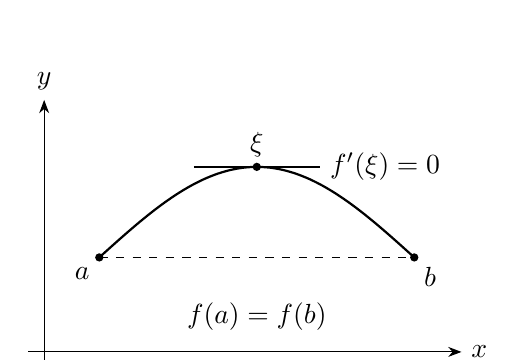
\begin{tikzpicture}[scale=1.0,>=Stealth]
  \draw[->] (-0.2,0)--(5.3,0) node[right] {$x$};
  \draw[->] (0,-0.2)--(0,3.2) node[above] {$y$};
  \draw[domain=0.7:4.7,smooth,variable=\x,thick]
    plot ({\x},{1.2+1.15*sin(45*(\x-0.7))});
  \coordinate (A) at (0.7,1.2);
  \coordinate (B) at (4.7,1.2);
  \coordinate (C) at (2.7,2.35);
  \fill (A) circle (1.5pt) node[below left] {$a$};
  \fill (B) circle (1.5pt) node[below right] {$b$};
  \fill (C) circle (1.5pt) node[above] {$\xi$};
  \draw[dashed] (A)--(B);
  \draw[thick] (1.9,2.35)--(3.5,2.35) node[right] {$f'(\xi)=0$};
  \node at (2.7,0.45) {$f(a)=f(b)$};
\end{tikzpicture}
\end{center}

\begin{theorem}[拉格朗日中值定理]
若 $f$ 在 $[a,b]$ 上连续，在 $(a,b)$ 内可导，则存在 $\xi\in(a,b)$，使得
\[
f'(\xi)=\frac{f(b)-f(a)}{b-a}.
\]
\end{theorem}
\begin{proofdetail}
构造辅助函数
\[
F(x)=f(x)-\frac{f(b)-f(a)}{b-a}(x-a).
\]
$F$ 在 $[a,b]$ 上连续，在 $(a,b)$ 内可导，且
\[
F(a)=f(a),\qquad F(b)=f(b)-[f(b)-f(a)]=f(a).
\]
由罗尔定理，存在 $\xi\in(a,b)$ 使 $F'(\xi)=0$。 而
\[
F'(x)=f'(x)-\frac{f(b)-f(a)}{b-a},
\]
故结论成立。
\end{proofdetail}

拉格朗日中值定理的几何意义是：连续光滑曲线上至少有一点的切线平行于连接两端点的弦。 公式
\[
f(b)-f(a)=f'(\xi)(b-a)
\]
说明“总改变量”等于某个中间点的瞬时变化率乘以区间长度。

\begin{center}
\begin{tikzpicture}[scale=1.0,>=Stealth]
  \draw[->] (-0.2,0)--(5.4,0) node[right] {$x$};
  \draw[->] (0,-0.2)--(0,4.0) node[above] {$y$};
  % y=0.18(x-2.2)^2+1, with a=0.8, b=4.6.
  % The secant slope equals f'(2.7)=0.18, so the tangent at xi=2.7 is parallel to the secant.
  \draw[domain=0.55:4.85,smooth,variable=\x,thick]
    plot ({\x},{0.18*(\x-2.2)*(\x-2.2)+1});
  \coordinate (A) at (0.8,1.353);
  \coordinate (B) at (4.6,2.037);
  \coordinate (C) at (2.7,1.045);
  \fill (A) circle (1.5pt) node[below left] {$(a,f(a))$};
  \fill (B) circle (1.5pt) node[above right] {$(b,f(b))$};
  \fill (C) circle (1.5pt) node[below] {$(\xi,f(\xi))$};
  \draw[thick,dashed] (A)--(B) node[midway,above,sloped] {弦};
  \draw[thick] ($(C)+(-1.2,-0.216)$)--($(C)+(1.2,0.216)$) node[right] {切线};
  \draw[dashed] (0.8,0)--(0.8,1.353);
  \draw[dashed] (2.7,0)--(2.7,1.045);
  \draw[dashed] (4.6,0)--(4.6,2.037);
  \node[below] at (0.8,0) {$a$};
  \node[below] at (2.7,0) {$\xi$};
  \node[below] at (4.6,0) {$b$};
\end{tikzpicture}
\end{center}

\begin{example}[验证中值定理]
对 $f(x)=x^2$ 在 $[1,3]$ 上求满足拉格朗日中值定理的 $\xi$。
\end{example}
\begin{solution}
\[
\frac{f(3)-f(1)}{3-1}=\frac{9-1}{2}=4.
\]
因 $f'(x)=2x$，令 $2\xi=4$ 得 $\xi=2\in(1,3)$。
\end{solution}

\begin{example}[罗尔定理的条件核查]
判断函数
\[
f(x)=|x|
\]
在区间 $[-1,1]$ 上能否应用罗尔定理。
\end{example}
\begin{solution}
首先，
\[
f(-1)=1,\qquad f(1)=1,
\]
两端函数值相等，且 $f$ 在 $[-1,1]$ 上连续。 但是 $f$ 在 $x=0$ 处不可导，因为
\[
\lim_{h\to0+}\frac{|h|-0}{h}=1,\qquad
\lim_{h\to0-}\frac{|h|-0}{h}=-1,
\]
左右导数不相等。 因此 $f$ 不满足“在 $(-1,1)$ 内可导”的条件，不能应用罗尔定理。
\end{solution}
\begin{warning}
罗尔定理的结论不是只由 $f(a)=f(b)$ 推出。 连续性和开区间可导性缺一不可，本题图像有尖点，正好破坏了可导性。
\end{warning}

\begin{example}[罗尔定理证明方程根的个数]
证明方程
\[
x^3-3x+1=0
\]
在区间 $(-2,2)$ 内有三个不同实根。
\end{example}
\begin{solution}
设
\[
f(x)=x^3-3x+1.
\]
计算得
\[
f(-2)=-1,\quad f(-1)=3,\quad f(0)=1,\quad f(1)=-1,\quad f(2)=3.
\]
由介值定理，区间 $(-2,-1)$、$(0,1)$、$(1,2)$ 内各至少有一个零点，所以 $(-2,2)$ 内至少有三个不同实根。

下面证明不可能有四个或更多不同实根。 若存在四个不同实根
\[
r_1<r_2<r_3<r_4,
\]
则在每个区间 $[r_i,r_{i+1}]$ 上，函数连续、开区间内可导，且两端函数值都为 $0$。 由罗尔定理，$f'$ 在 $(r_1,r_2)$、$(r_2,r_3)$、$(r_3,r_4)$ 内各至少有一个零点，因此 $f'$ 至少有三个不同零点。 但
\[
f'(x)=3x^2-3=3(x-1)(x+1)
\]
只有两个零点 $-1,1$，矛盾。 故方程在 $(-2,2)$ 内恰有三个不同实根。
\end{solution}

\begin{example}[构造辅助函数]
设 $f$ 在 $[0,1]$ 上连续，在 $(0,1)$ 内可导，且 $f(1)=0$。 证明存在 $\xi\in(0,1)$，使得
\[
f'(\xi)=-\frac{f(\xi)}{\xi}.
\]
\end{example}
\begin{solution}
令
\[
F(x)=xf(x).
\]
则 $F$ 在 $[0,1]$ 上连续，在 $(0,1)$ 内可导，并且
\[
F(0)=0,\qquad F(1)=f(1)=0.
\]
由罗尔定理，存在 $\xi\in(0,1)$，使得 $F'(\xi)=0$。 而
\[
F'(x)=f(x)+xf'(x),
\]
所以
\[
f(\xi)+\xi f'(\xi)=0.
\]
由于 $\xi\in(0,1)$，可除以 $\xi$，得到
\[
f'(\xi)=-\frac{f(\xi)}{\xi}.
\]
\end{solution}

\begin{example}[构造辅助函数]
设 $f$ 在 $[a,b]$ 上连续，在 $(a,b)$ 内可导，且 $f(a)=f(b)=0$。 证明存在 $\xi\in(a,b)$，使得
\[
f'(\xi)+f(\xi)=0.
\]
\end{example}
\begin{solution}
观察到表达式 $f'(x)+f(x)$ 是 $\ee^x f(x)$ 的导数中除去正因子后的部分。 令
\[
F(x)=\ee^x f(x).
\]
则 $F$ 在 $[a,b]$ 上连续，在 $(a,b)$ 内可导，并且
\[
F(a)=\ee^a f(a)=0,\qquad F(b)=\ee^b f(b)=0.
\]
由罗尔定理，存在 $\xi\in(a,b)$，使得 $F'(\xi)=0$。 而
\[
F'(x)=\ee^x f(x)+\ee^x f'(x)=\ee^x[f'(x)+f(x)].
\]
由于 $\ee^\xi>0$，所以
\[
f'(\xi)+f(\xi)=0.
\]
\end{solution}

\begin{example}[由导数界估计函数增量]
设 $f$ 在 $[a,b]$ 上连续，在 $(a,b)$ 内可导，且存在常数 $M>0$，使得
\[
|f'(x)|\leq M,\qquad x\in(a,b).
\]
证明对任意 $x_1,x_2\in[a,b]$，有
\[
|f(x_2)-f(x_1)|\leq M|x_2-x_1|.
\]
\end{example}
\begin{solution}
若 $x_1=x_2$，结论成立。 设 $x_1<x_2$。 由拉格朗日中值定理，存在 $\xi\in(x_1,x_2)$，使得
\[
f(x_2)-f(x_1)=f'(\xi)(x_2-x_1).
\]
取绝对值得
\[
|f(x_2)-f(x_1)|=|f'(\xi)|\,|x_2-x_1|\leq M|x_2-x_1|.
\]
当 $x_1>x_2$ 时交换两点即可。
\end{solution}

\begin{application}[物理：平均速度与瞬时速度]
设质点位置为 $s(t)$，单位分别为 $[s]=\mathrm m$、$[t]=\mathrm s$。若 $s$ 在 $[t_1,t_2]$ 上连续、在 $(t_1,t_2)$ 内可导，则拉格朗日中值定理保证存在 $\xi\in(t_1,t_2)$，使
\[
s'(\xi)=\frac{s(t_2)-s(t_1)}{t_2-t_1}.
\]
左边是时刻 $\xi$ 的瞬时速度，右边是该时间段的平均速度，二者单位均为 $\mathrm{m/s}$。因此，一段时间内的平均速度会在某个中间时刻真正取到。这里要求位置函数可导；若运动发生瞬时跳变，这一结论的条件便不满足。
\end{application}

\begin{application}[工程：传感器误差上界]
设温度传感器的标定函数为 $V(T)$，并假设在工作区间内
\[
|V'(T)|\leq0.02\ \mathrm{V/^{\circ}C}.
\]
若输入温度误差满足 $|\Delta T|\leq0.5\,^{\circ}\mathrm C$，则由中值定理，存在中间温度 $\xi$ 使
\[
|\Delta V|=|V'(\xi)|\,|\Delta T|
\leq0.02\times0.5
=0.01\ \mathrm V.
\]
这个估计把“灵敏度上界”转化为“输出误差上界”。它只计入由温度输入误差引起的变化；零点漂移、噪声等其他误差需要另行分析。
\end{application}

\subsection{柯西中值定理与若干推论}

\begin{theorem}[柯西中值定理]
若 $f,g$ 在 $[a,b]$ 上连续，在 $(a,b)$ 内可导，且 $g'(x)\neq0$ 对所有 $x\in(a,b)$ 成立，则存在 $\xi\in(a,b)$，使得
\[
\frac{f'(\xi)}{g'(\xi)}=\frac{f(b)-f(a)}{g(b)-g(a)}.
\]
\end{theorem}
\begin{proofdetail}
先说明 $g(b)\neq g(a)$。 若 $g(b)=g(a)$，由罗尔定理存在 $\eta\in(a,b)$ 使 $g'(\eta)=0$，与条件矛盾。

构造
\[
F(x)=f(x)-f(a)-\frac{f(b)-f(a)}{g(b)-g(a)}[g(x)-g(a)].
\]
则 $F$ 在 $[a,b]$ 连续，在 $(a,b)$ 可导，且 $F(a)=F(b)=0$。 由罗尔定理，存在 $\xi\in(a,b)$ 使 $F'(\xi)=0$。 即
\[
f'(\xi)-\frac{f(b)-f(a)}{g(b)-g(a)}g'(\xi)=0.
\]
因 $g'(\xi)\neq0$，除以 $g'(\xi)$ 得结论。
\end{proofdetail}

\begin{proposition}[导数恒为零的函数为常数]
若 $f$ 在区间 $I$ 上可导，且 $f'(x)=0$ 对所有 $x\in I$ 成立，则 $f$ 在 $I$ 上为常数。
\end{proposition}
\begin{proofdetail}
任取 $x_1,x_2\in I$，不妨 $x_1<x_2$。 $f$ 在 $[x_1,x_2]$ 连续、在 $(x_1,x_2)$ 可导。 由拉格朗日中值定理，存在 $\xi\in(x_1,x_2)$ 使
\[
f(x_2)-f(x_1)=f'(\xi)(x_2-x_1)=0.
\]
故任意两点函数值相等，$f$ 为常数。
\end{proofdetail}

\begin{proposition}[导数相等的函数相差常数]
若 $f,g$ 在区间 $I$ 上可导，且
\[
f'(x)=g'(x),\qquad x\in I,
\]
则存在常数 $C$，使得
\[
f(x)=g(x)+C,\qquad x\in I.
\]
\end{proposition}
\begin{proofdetail}
令 $h(x)=f(x)-g(x)$。 则 $h$ 在 $I$ 上可导，且
\[
h'(x)=f'(x)-g'(x)=0.
\]
由“导数恒为零的函数为常数”，$h(x)=C$。 即
\[
f(x)-g(x)=C.
\]
\end{proofdetail}

\begin{example}[柯西中值定理验证]
设
\[
f(x)=\ln x,\qquad g(x)=x,\qquad x\in[1,\ee].
\]
求柯西中值定理中的 $\xi$。
\end{example}
\begin{solution}
$f,g$ 在 $[1,\ee]$ 上连续，在 $(1,\ee)$ 内可导，且 $g'(x)=1\neq0$。柯西中值定理给出存在 $\xi\in(1,\ee)$，使
\[
\frac{f'(\xi)}{g'(\xi)}
=\frac{f(\ee)-f(1)}{g(\ee)-g(1)}.
\]
即
\[
\frac{1/\xi}{1}=\frac{1-0}{\ee-1}=\frac1{\ee-1}.
\]
因此
\[
\xi=\ee-1.
\]
由于 $1<\ee-1<\ee$，该点确在区间内部。
\end{solution}

\begin{example}[用柯西中值定理证明不等式]
证明当 $0<a<b$ 时，
\[
\frac{b-a}{b}<\ln b-\ln a<\frac{b-a}{a}.
\]
\end{example}
\begin{solution}
对 $f(x)=\ln x$ 和 $g(x)=x$ 在 $[a,b]$ 上应用柯西中值定理，存在 $\xi\in(a,b)$，使得
\[
\frac{\ln b-\ln a}{b-a}=\frac{f'(\xi)}{g'(\xi)}=\frac1{\xi}.
\]
因为 $a<\xi<b$，所以
\[
\frac1b<\frac1\xi<\frac1a.
\]
又 $b-a>0$，两边同乘以 $b-a$ 得
\[
\frac{b-a}{b}<\ln b-\ln a<\frac{b-a}{a}.
\]
\end{solution}

\begin{example}[不等式]
证明当 $x>0$ 时，$\ln(1+x)<x$。
\end{example}
\begin{solution}
令 $f(t)=\ln(1+t)$，在 $[0,x]$ 上应用拉格朗日中值定理，存在 $\xi\in(0,x)$ 使
\[
\ln(1+x)-\ln1=f'(\xi)x=\frac{x}{1+\xi}.
\]
因 $\xi>0$，有 $1+\xi>1$，故 $\ln(1+x)=x/(1+\xi)<x$。
\end{solution}

\begin{example}[不等式]
证明当 $x>0$ 时，
\[
\ln(1+x)>\frac{x}{1+x}.
\]
\end{example}
\begin{solution}
令
\[
F(x)=\ln(1+x)-\frac{x}{1+x},\qquad x\geq0.
\]
有 $F(0)=0$，且当 $x>0$ 时
\[
F'(x)=\frac1{1+x}-\frac1{(1+x)^2}
=\frac{x}{(1+x)^2}>0.
\]
由单调性判别法，$F$ 在 $[0,\infty)$ 上单调增加。 因此对 $x>0$，
\[
F(x)>F(0)=0,
\]
即
\[
\ln(1+x)>\frac{x}{1+x}.
\]
\end{solution}

\begin{example}[三角函数不等式]
证明当 $x>0$ 时，
\[
\sin x<x.
\]
\end{example}
\begin{solution}
当 $x\geq\pi$ 时，$\sin x\leq1<x$，结论成立。 下面只需考虑 $0<x<\pi$。

令 $f(t)=\sin t$，在 $[0,x]$ 上应用拉格朗日中值定理，存在 $\xi\in(0,x)$，使得
\[
\sin x-\sin0=f'(\xi)x=\cos\xi\,x.
\]
由于 $0<\xi<\pi$，有 $\cos\xi<1$，故
\[
\sin x=x\cos\xi<x.
\]
\end{solution}

\begin{example}[指数函数不等式]
证明对一切实数 $x$，
\[
\ee^x\geq1+x,
\]
且等号当且仅当 $x=0$。
\end{example}
\begin{solution}
令
\[
F(x)=\ee^x-1-x.
\]
则
\[
F'(x)=\ee^x-1.
\]
当 $x<0$ 时，$F'(x)<0$；当 $x>0$ 时，$F'(x)>0$。 因而 $F$ 在 $(-\infty,0)$ 上单调减少，在 $(0,\infty)$ 上单调增加，所以 $x=0$ 是全局最小点。 又
\[
F(0)=0.
\]
于是 $F(x)\geq0$，即
\[
\ee^x\geq1+x.
\]
当 $x\neq0$ 时，$F(x)>F(0)=0$，故等号仅当 $x=0$ 成立。
\end{solution}

\subsection{洛必达法则}

\begin{theorem}[洛必达法则：$0/0$ 型]
设 $f,g$ 在 $a$ 的某去心右邻域内可导，且 $g'(x)\neq0$。 若
\[
\lim_{x\to a+}f(x)=\lim_{x\to a+}g(x)=0,\qquad
\lim_{x\to a+}\frac{f'(x)}{g'(x)}=L
\]
其中 $L$ 可为有限数或无穷大，则
\[
\lim_{x\to a+}\frac{f(x)}{g(x)}=L.
\]
左极限、双侧极限与 $x\to\infty$ 的相应形式类似成立。
\end{theorem}
\begin{proofdetail}
先证 $L$ 为有限数的情形。 任取 $\varepsilon>0$，由 $\frac{f'}{g'}\to L$，存在 $\delta>0$，当 $a<x<a+\delta$ 时，
\[
L-\varepsilon<\frac{f'(x)}{g'(x)}<L+\varepsilon.
\]
取 $x\in(a,a+\delta)$，再取 $t\in(a,x)$。 在 $[t,x]$ 上对 $f,g$ 应用柯西中值定理，存在 $\xi\in(t,x)$ 使
\[
\frac{f(x)-f(t)}{g(x)-g(t)}=\frac{f'(\xi)}{g'(\xi)}.
\]
因此
\[
\left|\frac{f(x)-f(t)}{g(x)-g(t)}-L\right|<\varepsilon.
\]
固定 $x$ 后令 $t\to a+$，由 $f(t)\to0,g(t)\to0$ 得
\[
\left|\frac{f(x)}{g(x)}-L\right|\leq\varepsilon
\]
其中 $x\in(a,a+\delta)$ 且 $g(x)\neq0$。 因 $\varepsilon$ 任意，得 $\frac{f(x)}{g(x)}\to L$。

若 $L=+\infty$，任取 $M>0$，可令 $\delta>0$ 充分小，使 $a<x<a+\delta$ 时 $\frac{f'(x)}{g'(x)}>2M$。重复上面的柯西中值定理步骤，先得到相应差商大于 $2M$，再令 $t\to a+$，可得 $\frac{f(x)}{g(x)}\geq2M>M$，故极限为 $+\infty$。若 $L=-\infty$，同理使用 $\frac{f'}{g'}<-2M$，得到 $\frac{f(x)}{g(x)}\leq-2M<-M$。
\end{proofdetail}

\begin{theorem}[洛必达法则：$\infty/\infty$ 型]
设 $f,g$ 在 $a$ 的某去心右邻域内可导，且 $g'(x)\neq0$。 若
\[
\lim_{x\to a+}|f(x)|=+\infty,\qquad
\lim_{x\to a+}|g(x)|=+\infty,
\]
并且
\[
\lim_{x\to a+}\frac{f'(x)}{g'(x)}=L,
\]
其中 $L$ 可为有限数或无穷大，则
\[
\lim_{x\to a+}\frac{f(x)}{g(x)}=L.
\]
左极限、双侧极限与 $x\to\infty$ 的相应形式类似成立。
\end{theorem}
\begin{proofdetail}
证明有限 \(L\) 的情形。任取 \(\varepsilon>0\)，由 \(\frac{f'}{g'}\to L\)，存在 \(\delta>0\)，使得任意 \(u\in(a,a+\delta)\) 都满足
\[
\left|\frac{f'(u)}{g'(u)}-L\right|<\varepsilon.
\]
固定 \(x_0\in(a,a+\delta)\)。对任意 \(x\in(a,x_0)\)，在 \([x,x_0]\) 上应用柯西中值定理，存在 \(\xi\in(x,x_0)\subset(a,a+\delta)\)，使
\[
\frac{f(x)-f(x_0)}{g(x)-g(x_0)}=\frac{f'(\xi)}{g'(\xi)}.
\]
因此
\[
\left|\frac{f(x)-f(x_0)}{g(x)-g(x_0)}-L\right|<\varepsilon.
\]
另一方面，
\[
\frac{f(x)}{g(x)}
=\frac{f(x)-f(x_0)}{g(x)-g(x_0)}
\left(1-\frac{g(x_0)}{g(x)}\right)
+\frac{f(x_0)}{g(x)}.
\]
当 \(x\to a+\) 时，后两个因子分别趋于 \(1\) 和 \(0\)。由上式与 \(\varepsilon\) 的任意性可得 \(\frac{f(x)}{g(x)}\to L\)。

若 \(L=+\infty\)，任取 \(M>0\)，令 \(x\) 充分接近 \(a\)，使柯西中值定理给出的差商大于 \(4M\)，并且
\[
1-\frac{g(x_0)}{g(x)}>\frac12,
\qquad
\left|\frac{f(x_0)}{g(x)}\right|<M.
\]
代入上式即得 \(\frac{f(x)}{g(x)}>4M\cdot\frac12-M=M\)，所以 \(\frac{f(x)}{g(x)}\to+\infty\)。若 \(L=-\infty\)，使用差商小于 \(-4M\) 的同样估计，可得 \(\frac{f(x)}{g(x)}<-M\)。
\end{proofdetail}

\begin{warning}
洛必达法则只给出一组充分条件，不能反向使用。即使 \(\lim f(x)/g(x)\) 存在，\(\lim f'(x)/g'(x)\) 也可能不存在；使用法则前还必须先确认原式确为 \(0/0\) 型或 \(\infty/\infty\) 型。
\end{warning}

\begin{example}[$0/0$ 型]
求 $\displaystyle\lim_{x\to0}\frac{\sin x}{x}$。
\end{example}
\begin{solution}
这是 $0/0$ 型。 用洛必达法则：
\[
\lim_{x\to0}\frac{\sin x}{x}=\lim_{x\to0}\frac{\cos x}{1}=1.
\]
\end{solution}

\begin{example}[多次使用]
求 $\displaystyle\lim_{x\to0}\frac{\ee^x-1-x}{x^2}$。
\end{example}
\begin{solution}
第一次洛必达：
\[
\lim_{x\to0}\frac{\ee^x-1-x}{x^2}
=\lim_{x\to0}\frac{\ee^x-1}{2x}.
\]
仍为 $0/0$ 型，第二次洛必达：
\[
=\lim_{x\to0}\frac{\ee^x}{2}=\frac12.
\]
\end{solution}
\begin{warning}
使用洛必达前必须确认是 $0/0$ 或 $\infty/\infty$ 型，并确认分母导数不为零的条件在去心邻域内成立。
\end{warning}

\begin{example}[$\infty/\infty$ 型]
求
\[
\lim_{x\to\infty}\frac{\ln x}{x^\alpha},\qquad \alpha>0.
\]
\end{example}
\begin{solution}
当 $x\to\infty$ 时，分子、分母都趋于 $+\infty$，属于 $\infty/\infty$ 型。 用洛必达法则：
\[
\lim_{x\to\infty}\frac{\ln x}{x^\alpha}
=\lim_{x\to\infty}\frac{1/x}{\alpha x^{\alpha-1}}
=\lim_{x\to\infty}\frac{1}{\alpha x^\alpha}=0.
\]
这说明任意正幂函数 $x^\alpha$ 的增长都快于 $\ln x$。
\end{solution}

\begin{example}[三角函数高阶小量]
求
\[
\lim_{x\to0}\frac{\tan x-x}{x^3}.
\]
\end{example}
\begin{solution}
这是 $0/0$ 型。 第一次洛必达：
\[
\lim_{x\to0}\frac{\tan x-x}{x^3}
=\lim_{x\to0}\frac{\sec^2x-1}{3x^2}
=\lim_{x\to0}\frac{\tan^2x}{3x^2}.
\]
因为 $\lim_{x\to0}\frac{\tan x}{x}=1$，所以
\[
\lim_{x\to0}\frac{\tan^2x}{3x^2}
=\frac13.
\]
\end{solution}

\begin{example}[不能机械使用洛必达法则]
讨论 $\displaystyle\lim_{x\to\infty}\frac{x+\sin x}{x+\cos x}$。
\end{example}
\begin{solution}
这是 $\infty/\infty$ 型，但直接看导数之比会得到
\[
\frac{(x+\sin x)'}{(x+\cos x)'}=\frac{1+\cos x}{1-\sin x},
\]
该式当 $x\to\infty$ 时无极限，因此不能由洛必达法则推出原极限不存在。 原式应先整理：
\[
\frac{x+\sin x}{x+\cos x}
=\frac{1+\frac{\sin x}{x}}{1+\frac{\cos x}{x}}.
\]
由于 $\sin x/x\to0,\ \cos x/x\to0$，原极限为 $1$。
\end{solution}
\begin{warning}
洛必达法则给出的是充分条件：若导数之比的极限存在，原比值极限等于它。 导数之比极限不存在时，原极限仍可能存在。
\end{warning}

\begin{example}[转化未定式]
求 $\displaystyle\lim_{x\to0+}x\ln x$。
\end{example}
\begin{solution}
原式为 $0\cdot(-\infty)$ 型，改写为
\[
x\ln x=\frac{\ln x}{1/x}.
\]
当 $x\to0+$ 时为 $-\infty/\infty$ 型。 用洛必达法则：
\[
\lim_{x\to0+}\frac{\ln x}{1/x}
=\lim_{x\to0+}\frac{1/x}{-1/x^2}
=\lim_{x\to0+}(-x)=0.
\]
\end{solution}

\begin{example}[指数型未定式]
求
\[
\lim_{x\to0+}x^x.
\]
\end{example}
\begin{solution}
原式为 $0^0$ 型。 设
\[
y=x^x.
\]
取对数得
\[
\ln y=x\ln x.
\]
由上一例，
\[
\lim_{x\to0+}x\ln x=0.
\]
因此
\[
\lim_{x\to0+}\ln y=0.
\]
由于指数函数连续，
\[
\lim_{x\to0+}x^x=\ee^0=1.
\]
\end{solution}

\begin{example}[差型未定式]
求
\[
\lim_{x\to0+}\left(\frac1x-\frac1{\ee^x-1}\right).
\]
\end{example}
\begin{solution}
原式为 $\infty-\infty$ 型，先通分：
\[
\frac1x-\frac1{\ee^x-1}
=\frac{\ee^x-1-x}{x(\ee^x-1)}.
\]
当 $x\to0+$ 时为 $0/0$ 型。 用洛必达法则：
\[
\lim_{x\to0+}\frac{\ee^x-1-x}{x(\ee^x-1)}
=\lim_{x\to0+}\frac{\ee^x-1}{\ee^x-1+x\ee^x}.
\]
仍为 $0/0$ 型，再用一次洛必达：
\[
=\lim_{x\to0+}\frac{\ee^x}{2\ee^x+x\ee^x}
=\frac12.
\]
\end{solution}

\begin{example}[参数型极限]
设 $a>0$。 求
\[
\lim_{x\to0}\frac{a^x-1}{x}.
\]
\end{example}
\begin{solution}
当 $x\to0$ 时为 $0/0$ 型。 由洛必达法则，
\[
\lim_{x\to0}\frac{a^x-1}{x}
=\lim_{x\to0}\frac{a^x\ln a}{1}
=\ln a.
\]
特别地，当 $a=\ee$ 时，得到
\[
\lim_{x\to0}\frac{\ee^x-1}{x}=1.
\]
\end{solution}

\subsection{函数单调性判别法}

\begin{theorem}[单调性判别法]
设 $f$ 在区间 $I$ 上连续，在 $I$ 的内部可导。 若 $f'(x)\geq0$ 对内部所有点成立，则 $f$ 在 $I$ 上单调不减；若 $f'(x)>0$ 对内部所有点成立，则 $f$ 在 $I$ 上严格单调增加。 相应地，$f'(x)\leq0$ 推出单调不增，$f'(x)<0$ 推出严格单调减少。
\end{theorem}
\begin{proofdetail}
任取 $x_1<x_2$，由拉格朗日中值定理，存在 $\xi\in(x_1,x_2)$，使
\[
f(x_2)-f(x_1)=f'(\xi)(x_2-x_1).
\]
若 $f'\geq0$，则右端 $\geq0$，故 $f(x_2)\geq f(x_1)$。 若 $f'>0$，则右端 $>0$，故严格增加。 其余情形同理。
\end{proofdetail}

\begin{example}[求单调区间]
求 $f(x)=x^3-3x$ 的单调区间。
\end{example}
\begin{solution}
\[
f'(x)=3x^2-3=3(x-1)(x+1).
\]
当 $x<-1$ 或 $x>1$ 时 $f'(x)>0$；当 $-1<x<1$ 时 $f'(x)<0$。 故 $f$ 在 $(-\infty,-1)$ 与 $(1,\infty)$ 上单调增加，在 $(-1,1)$ 上单调减少。
\end{solution}

\begin{example}[求单调区间]
求函数
\[
f(x)=2x^3-9x^2+12x-3
\]
的单调区间。
\end{example}
\begin{solution}
\[
f'(x)=6x^2-18x+12=6(x-1)(x-2).
\]
临界点为 $x=1,2$。 当 $x<1$ 时 $f'(x)>0$；当 $1<x<2$ 时 $f'(x)<0$；当 $x>2$ 时 $f'(x)>0$。 因此 $f$ 在 $(-\infty,1)$ 与 $(2,\infty)$ 上单调增加，在 $(1,2)$ 上单调减少。
\end{solution}

\subsection{函数的极值}

\begin{definition}[局部极值]
若存在 $\delta>0$，使得对所有满足 $|x-x_0|<\delta$ 的 $x$，都有 $f(x)\leq f(x_0)$，则称 $f(x_0)$ 为局部极大值。 若不等号反向，则称为局部极小值。
\end{definition}

\begin{theorem}[一阶导数变号判别法]
设 $f$ 在 $x_0$ 连续，在 $x_0$ 的去心邻域内可导。 若 $f'$ 在 $x_0$ 左侧为正、右侧为负，则 $f(x_0)$ 为局部极大值；若左侧为负、右侧为正，则为局部极小值。 若在 $x_0$ 左右两侧，$f'$ 保持相同的严格符号，即两侧均有 $f'(x)>0$ 或两侧均有 $f'(x)<0$，则 $x_0$ 不是极值点。
\end{theorem}
\begin{proofdetail}
只证由正变负的情形。 存在 $\delta>0$，使 $f'(x)>0$ 对 $x\in(x_0-\delta,x_0)$ 成立，$f'(x)<0$ 对 $x\in(x_0,x_0+\delta)$ 成立。 由单调性判别法，$f$ 在左侧区间单调增加，在右侧区间单调减少。 因 $f$ 在 $x_0$ 连续，对任意 $x\in(x_0-\delta,x_0)$ 有 $f(x)<f(x_0)$，对任意 $x\in(x_0,x_0+\delta)$ 有 $f(x)<f(x_0)$。 因此 $f(x_0)$ 为局部极大值。 其余情形同理。
\end{proofdetail}

\begin{theorem}[二阶导数判别法]
设 $f'(x_0)=0$，且 $f''(x_0)$ 存在。 若 $f''(x_0)>0$，则 $f(x_0)$ 是局部极小值；若 $f''(x_0)<0$，则是局部极大值。
\end{theorem}
\begin{proofdetail}
由二阶导数定义，
\[
f''(x_0)=\lim_{x\to x_0}\frac{f'(x)-f'(x_0)}{x-x_0}
=\lim_{x\to x_0}\frac{f'(x)}{x-x_0}.
\]
若 $f''(x_0)>0$，则存在 $\delta>0$，当 $0<|x-x_0|<\delta$ 时
\[
\frac{f'(x)}{x-x_0}>0.
\]
于是 $x<x_0$ 时 $f'(x)<0$，$x>x_0$ 时 $f'(x)>0$，由一阶变号判别法得局部极小。 $f''(x_0)<0$ 时同理得到导数由正变负，故为局部极大。
\end{proofdetail}

\begin{example}[极值]
求 $f(x)=x^4-4x^3$ 的极值。
\end{example}
\begin{solution}
\[
f'(x)=4x^3-12x^2=4x^2(x-3).
\]
临界点为 $x=0,3$。 因 $x^2\geq0$，$f'(x)$ 在 $0$ 两侧均为负，所以 $x=0$ 不是极值点。 $f'$ 在 $3$ 左侧负、右侧正，故 $x=3$ 为局部极小点，
\[
f(3)=81-108=-27.
\]
\end{solution}
\begin{warning}
导数为零只是极值的必要条件，不是充分条件。 $x=0$ 就是典型反例。
\end{warning}

\begin{example}[极值]
求函数
\[
f(x)=(x-1)^2(x+1)^3
\]
的极值。
\end{example}
\begin{solution}
求导得
\[
f'(x)=2(x-1)(x+1)^3+3(x-1)^2(x+1)^2
=(x-1)(x+1)^2(5x-1).
\]
临界点为 $x=-1,\frac15,1$。 由于 $(x+1)^2\geq0$，且除 $x=-1$ 外不改变符号，只需考察 $(x-1)(5x-1)$ 的符号，并注意 $x=-1$ 两侧符号是否改变。

当 $x<\frac15$ 且 $x\neq-1$ 时，$(x-1)<0,\ 5x-1<0$，故 $f'(x)>0$；当 $\frac15<x<1$ 时，$f'(x)<0$；当 $x>1$ 时，$f'(x)>0$。 因而 $x=-1$ 不是极值点，$x=\frac15$ 为局部极大点，$x=1$ 为局部极小点。

函数值为
\[
f\left(\frac15\right)=\left(-\frac45\right)^2\left(\frac65\right)^3=\frac{3456}{3125},\qquad
f(1)=0.
\]
故局部极大值为 $\frac{3456}{3125}$，局部极小值为 $0$。
\end{solution}

\subsection{函数的最值与应用优化}

\begin{proposition}[闭区间最值求法]
若 $f$ 在 $[a,b]$ 连续，则最大值和最小值只能在端点、不可导点或内部驻点 $f'(x)=0$ 处取得。 逐一比较这些点的函数值即可。
\end{proposition}
\begin{proofdetail}
最值存在性来自闭区间连续函数最值定理。 若最值在内部点 $x_0$ 取得且 $f$ 在 $x_0$ 可导，则由费马引理 $f'(x_0)=0$。 若内部点不可导，也必须列入候选。 端点处费马引理不适用，因此端点也必须比较。
\end{proofdetail}

\begin{example}[利润最大化]
某产品价格与销量满足 $p(q)=100-q$，成本 $C(q)=20q+100$，其中 $0\leq q\leq100$。 求最大利润。
\end{example}
\begin{solution}
收入 $R(q)=qp(q)=100q-q^2$，利润
\[
\Pi(q)=R(q)-C(q)=80q-q^2-100.
\]
\[
\Pi'(q)=80-2q.
\]
令 $\Pi'(q)=0$ 得 $q=40$。 比较
\[
\Pi(0)=-100,\quad \Pi(40)=1600-100=1500,\quad \Pi(100)=8000-10000-100=-2100.
\]
最大利润为 $1500$，在 $q=40$ 时取得。
\end{solution}

\begin{example}[证明方程根的个数]
证明方程 $x^3-3x+1=0$ 在区间 $(-2,2)$ 内有三个不同实根。
\end{example}
\begin{solution}
设 $f(x)=x^3-3x+1$。 有
\[
f(-2)=-1,\quad f(-1)=3,\quad f(0)=1,\quad f(1)=-1,\quad f(2)=3.
\]
由介值定理，$(-2,-1)$、$(0,1)$、$(1,2)$ 内各至少有一个根。

再证至多三个根。 若有四个不同实根 $r_1<r_2<r_3<r_4$，由罗尔定理，$f'$ 在三个相邻根之间至少有三个不同零点。 但
\[
f'(x)=3x^2-3
\]
只有两个零点 $\pm1$，矛盾。 故恰有三个不同实根。
\end{solution}

\begin{application}[农业：简化的最佳施肥量模型]
设 $N$ 为每公顷氮肥投入量，单位为 $\mathrm{kg/ha}$；$Y(N)$ 为作物产量，单位为 $\mathrm{t/ha}$。在给定品种、土壤和水分条件近似不变的一个有限试验范围内，用教学模型
\[
Y(N)=Y_0+aN-bN^2,\qquad a,b>0
\]
描述边际增产逐渐减弱的情形。由
\[
Y'(N)=a-2bN,\qquad Y''(N)=-2b<0
\]
可知唯一内部临界点
\[
N_*=\frac{a}{2b}
\]
在模型范围内对应产量极大值。该结论展示了导数求最值的方法，并不是生产处方：真实产量还受土壤、水分、品种、天气、病虫害及水肥交互作用影响，模型参数也必须由试验数据估计。\upcite{TaizPlant}
\end{application}

\subsection{曲线的凸性与拐点}

\begin{definition}[曲线的上凸与下凸]
设曲线 $y=f(x)$ 在区间 $(a,b)$ 内每一点都有切线。 若曲线上任意一点处的切线都在曲线的上方，则称曲线在 $(a,b)$ 内为\textbf{上凸}；若曲线上任意一点处的切线都在曲线的下方，则称曲线在 $(a,b)$ 内为\textbf{下凸}。

教材之间关于“凸”“凹”的命名不完全一致。 本讲义在本节采用曲线的上凸、下凸说法，避免与现代凸分析中“凸函数”定义混淆。
\end{definition}

\begin{center}
\begin{tikzpicture}[scale=0.95,>=Stealth]
  \begin{scope}
    \draw[->] (-2.1,0)--(2.2,0) node[right] {$x$};
    \draw[->] (0,-0.3)--(0,2.7) node[above] {$y$};
    \draw[domain=-1.65:1.65,smooth,variable=\x,thick]
      plot ({\x},{0.42*\x*\x+0.45});
    \coordinate (P) at (0.75,0.686);
    \draw[thick] ($(P)+(-1.35,-0.851)$)--($(P)+(1.35,0.851)$);
    \fill (P) circle (1.5pt);
    \node at (0,-0.65) {下凸：切线在曲线下方};
  \end{scope}
  \begin{scope}[xshift=7cm]
    \draw[->] (-2.1,0)--(2.2,0) node[right] {$x$};
    \draw[->] (0,-0.3)--(0,2.7) node[above] {$y$};
    \draw[domain=-1.65:1.65,smooth,variable=\x,thick]
      plot ({\x},{2.25-0.42*\x*\x});
    \coordinate (Q) at (0.75,2.014);
    \draw[thick] ($(Q)+(-1.35,0.851)$)--($(Q)+(1.35,-0.851)$);
    \fill (Q) circle (1.5pt);
    \node at (0,-0.65) {上凸：切线在曲线上方};
  \end{scope}
\end{tikzpicture}
\end{center}

\begin{theorem}[二阶导数判别凸性]
若 $f$ 在 $(a,b)$ 内二阶可导，则：
\[
f''(x)>0\quad (x\in(a,b))\quad\Longrightarrow\quad y=f(x)\text{ 在 }(a,b)\text{ 内下凸};
\]
\[
f''(x)<0\quad (x\in(a,b))\quad\Longrightarrow\quad y=f(x)\text{ 在 }(a,b)\text{ 内上凸}.
\]
\end{theorem}
\begin{proofdetail}
只证 $f''>0$ 的情形。 任取 $x_0\in(a,b)$，点 $(x_0,f(x_0))$ 处切线为
\[
T(x)=f(x_0)+f'(x_0)(x-x_0).
\]
令
\[
F(x)=f(x)-T(x).
\]
则 $F(x_0)=0,\ F'(x_0)=0$，且
\[
F''(x)=f''(x)>0.
\]
由单调性判别法，$F'$ 在 $(a,b)$ 内严格增加。 因 $F'(x_0)=0$，当 $x<x_0$ 时 $F'(x)<0$，当 $x>x_0$ 时 $F'(x)>0$。 因此 $F$ 在 $x_0$ 左侧随 $x$ 增大而减少，在 $x_0$ 右侧随 $x$ 增大而增加。 对任意 $x\neq x_0$，都有 $F(x)>F(x_0)=0$，即
\[
f(x)>f(x_0)+f'(x_0)(x-x_0).
\]
这说明切线在曲线下方，故曲线下凸。 若 $f''<0$，则对 $-f$ 应用已证结论，得到原曲线切线在曲线上方，故上凸。
\end{proofdetail}

\begin{definition}[拐点]
若曲线 $y=f(x)$ 在点 $x_0$ 的两侧凸凹性发生改变，则称 $(x_0,f(x_0))$ 为曲线的拐点。
\end{definition}

\begin{center}
\begin{tikzpicture}[scale=1.0,>=Stealth]
  \draw[->] (-2.6,0)--(2.7,0) node[right] {$x$};
  \draw[->] (0,0.2)--(0,3.4) node[above] {$y$};
  \draw[domain=-2.05:2.05,smooth,variable=\x,thick]
    plot ({\x},{1.75+0.18*\x*\x*\x});
  \coordinate (I) at (0,1.75);
  \fill (I) circle (1.5pt) node[above left] {拐点};
  \draw[dashed] (0,0)--(I);
  \node at (-1.55,2.55) {上凸};
  \node at (1.45,1.0) {下凸};
  \node[below] at (0,0) {$x_0$};
\end{tikzpicture}
\end{center}

\begin{example}[凸性与拐点]
讨论 $f(x)=x^3-3x$ 的凸性与拐点。
\end{example}
\begin{solution}
\[
f''(x)=6x.
\]
当 $x<0$ 时 $f''(x)<0$，曲线上凸；当 $x>0$ 时 $f''(x)>0$，曲线下凸。 上凸、下凸性在 $x=0$ 改变，故 $(0,0)$ 是拐点。
\end{solution}

\begin{example}[凸性与拐点]
求曲线
\[
y=2x^3+3x^2+12x+14
\]
的上凸区间、下凸区间和拐点。
\end{example}
\begin{solution}
\[
y'=6x^2+6x+12,\qquad y''=12x+6=6(2x+1).
\]
令 $y''=0$ 得 $x=-\frac12$。 当 $x<-\frac12$ 时 $y''<0$，曲线上凸；当 $x>-\frac12$ 时 $y''>0$，曲线下凸。 因此上凸区间为
\[
\left(-\infty,-\frac12\right),
\]
下凸区间为
\[
\left(-\frac12,\infty\right).
\]
又
\[
y\left(-\frac12\right)=2\left(-\frac18\right)+3\left(\frac14\right)+12\left(-\frac12\right)+14
=\frac{17}{2}.
\]
所以拐点为
\[
\left(-\frac12,\frac{17}{2}\right).
\]
\end{solution}

\subsection{曲线的渐近线与函数图像}

\begin{definition}[渐近线]
若
\[
\lim_{x\to x_0^-}f(x)=+\infty,\quad
\lim_{x\to x_0^-}f(x)=-\infty,\quad
\lim_{x\to x_0^+}f(x)=+\infty,\quad
\lim_{x\to x_0^+}f(x)=-\infty
\]
四种情形中至少有一种成立，则 $x=x_0$ 为垂直渐近线。若 $\lim_{x\to+\infty}f(x)=b$ 或 $\lim_{x\to-\infty}f(x)=b$，则 $y=b$ 是相应方向上的水平渐近线。若存在 $a,b$ 使
\[
\lim_{x\to+\infty}[f(x)-(ax+b)]=0
\]
则 $y=ax+b$ 为 $x\to+\infty$ 时的斜渐近线；$x\to-\infty$ 时同理。
\end{definition}

\begin{center}
\begin{tikzpicture}[scale=0.95,>=Stealth]
  \begin{scope}
    \draw[->] (-1.6,0)--(3.2,0) node[right] {$x$};
    \draw[->] (0,-1.1)--(0,3.0) node[above] {$y$};
    \draw[dashed] (1,-1.0)--(1,2.8) node[above] {$x=x_0$};
    \draw[dashed] (-1.5,1)--(3.0,1) node[right] {$y=b$};
    \draw[domain=-1.4:0.72,smooth,variable=\x,thick]
      plot ({\x},{1+0.55/(\x-1)});
    \draw[domain=1.28:3.0,smooth,variable=\x,thick]
      plot ({\x},{1+0.55/(\x-1)});
    \node at (0.75,-1.45) {垂直渐近线与水平渐近线};
  \end{scope}
  \begin{scope}[xshift=7.0cm]
    \draw[->] (-1.6,0)--(3.3,0) node[right] {$x$};
    \draw[->] (0,-1.0)--(0,3.2) node[above] {$y$};
    \draw[dashed] (-1.3,-0.2)--(3.0,2.8) node[right] {$y=ax+b$};
    \draw[domain=-1.25:3.0,smooth,variable=\x,thick]
      plot ({\x},{0.7*\x+0.7+0.55/(\x*\x+1.2)});
    \node at (0.75,-1.45) {斜渐近线};
  \end{scope}
\end{tikzpicture}
\end{center}

\begin{proposition}[斜渐近线求法]
若
\[
a=\lim_{x\to\infty}\frac{f(x)}{x},\qquad
b=\lim_{x\to\infty}[f(x)-ax]
\]
均存在且有限，则 $y=ax+b$ 是 $x\to\infty$ 时的斜渐近线。
\end{proposition}
\begin{proofdetail}
由 $b$ 的定义，
\[
\lim_{x\to\infty}[f(x)-(ax+b)]
=\lim_{x\to\infty}\{[f(x)-ax]-b\}=0.
\]
这正是斜渐近线定义。 其中 $a$ 的公式来自若 $f(x)-(ax+b)\to0$，则
\[
\frac{f(x)}x-a-\frac bx\to0,
\]
因此 $f(x)/x\to a$。
\end{proofdetail}

\begin{example}[完整图像分析]
讨论 $f(x)=\frac{x^2}{x-1}$ 的单调性、极值与渐近线。
\end{example}
\begin{solution}
定义域为 $(-\infty,1)\cup(1,\infty)$。 垂直渐近线：$x=1$。
作除法：
\[
\frac{x^2}{x-1}=x+1+\frac1{x-1},
\]
故斜渐近线为 $y=x+1$。

求导：
\[
f'(x)=\frac{2x(x-1)-x^2}{(x-1)^2}=\frac{x(x-2)}{(x-1)^2}.
\]
因分母为正，符号由 $x(x-2)$ 决定。 故在 $(-\infty,0)$、$(2,\infty)$ 上增加，在 $(0,1)$、$(1,2)$ 上减少。 $x=0$ 处导数由正变负，为局部极大，$f(0)=0$；$x=2$ 处导数由负变正，为局部极小，$f(2)=4$。
\end{solution}

\begin{center}
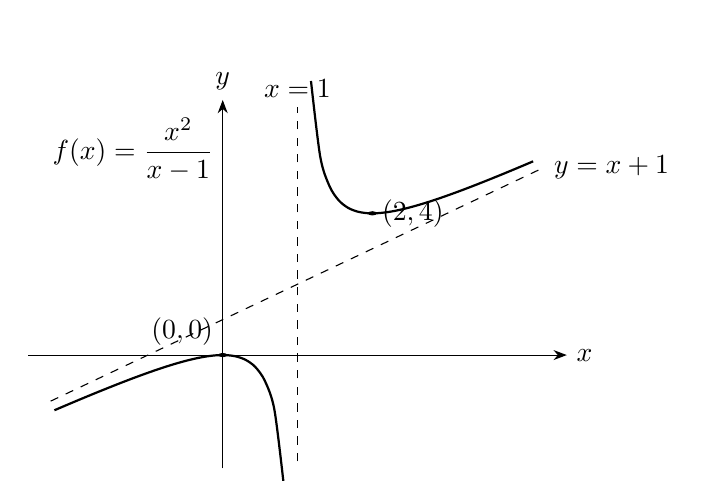
\begin{tikzpicture}[xscale=0.95,yscale=0.45,>=Stealth]
  \draw[->] (-2.6,0)--(4.6,0) node[right] {$x$};
  \draw[->] (0,-3.2)--(0,7.2) node[above] {$y$};
  \draw[dashed] (1,-3.0)--(1,7.0) node[above] {$x=1$};
  \draw[dashed] (-2.3,-1.3)--(4.3,5.3) node[right] {$y=x+1$};
  \draw[domain=-2.25:0.82,smooth,variable=\x,thick]
    plot ({\x},{\x+1+1/(\x-1)});
  \draw[domain=1.18:4.15,smooth,variable=\x,thick]
    plot ({\x},{\x+1+1/(\x-1)});
  \fill (0,0) circle (1.7pt) node[above left] {$(0,0)$};
  \fill (2,4) circle (1.7pt) node[right] {$(2,4)$};
  \node at (-1.2,5.8) {$f(x)=\dfrac{x^2}{x-1}$};
\end{tikzpicture}
\end{center}


\begin{application}[凸性与机器学习优化]
	凸性在优化问题中非常重要。 直观地说，凸函数的图像没有“局部低谷冒充全局最低点”的现象。 在一元情形下，若 $f''(x)\ge0$，则 $f$ 为下凸函数；若严格凸且存在临界点，那么该临界点就是全局最小点。 许多基础机器学习模型，例如线性回归的均方误差损失，关于参数是凸函数，因此可以用导数和梯度方法稳定地寻找最优参数。
	
	\begin{example}
		设单样本线性模型损失为
		\[
		L(w)=\frac12(wx-y)^2,
		\]
		其中 $x,y$ 为常数。 讨论 $L$ 关于 $w$ 的凸性。
	\end{example}
	\begin{solution}
		对 $w$ 求导：
		\[
		L'(w)=x(wx-y),\qquad L''(w)=x^2\ge0.
		\]
		因此 $L$ 关于 $w$ 是下凸函数。 若 $x\neq0$，则 $L''(w)=x^2>0$，函数严格凸，唯一最小点由 $L'(w)=0$ 给出，即
		\[
		w=\frac{y}{x}.
		\]
		若 $x=0$，则 $L(w)=\frac12y^2$ 为常数函数，任意 $w$ 都是最小点。
	\end{solution}
	
\end{application}




\subsection{泰勒公式}

\begin{theorem}[泰勒公式：拉格朗日余项]
若 $f$ 在含 $x_0$ 与 $x$ 的区间上有 $n+1$ 阶连续导数，则存在介于 $x_0$ 与 $x$ 之间的 $\xi$，使得
\[
f(x)=\sum_{k=0}^{n}\frac{f^{(k)}(x_0)}{k!}(x-x_0)^k
+\frac{f^{(n+1)}(\xi)}{(n+1)!}(x-x_0)^{n+1}.
\]
\end{theorem}
\begin{proofdetail}
记
\[
P_n(t)=\sum_{k=0}^{n}\frac{f^{(k)}(x_0)}{k!}(t-x_0)^k.
\]
固定 $x\neq x_0$，令
\[
R=f(x)-P_n(x),\qquad
M=\frac{R}{(x-x_0)^{n+1}}.
\]
构造
\[
F(t)=f(t)-P_n(t)-M(t-x_0)^{n+1}.
\]
由 $P_n$ 的构造可知
\[
F(x_0)=F'(x_0)=\cdots=F^{(n)}(x_0)=0,
\]
且由 $M$ 的定义，$F(x)=0$。 对 $F$ 在以 $x_0,x$ 为端点的区间反复使用罗尔定理：由 $F(x_0)=F(x)=0$，存在一点使 $F'=0$；又 $F'(x_0)=0$，可在相应子区间再次使用罗尔定理，逐次得到存在 $\xi$ 介于 $x_0$ 与 $x$ 之间，使
\[
F^{(n+1)}(\xi)=0.
\]
而
\[
F^{(n+1)}(t)=f^{(n+1)}(t)-M(n+1)!.
\]
故
\[
M=\frac{f^{(n+1)}(\xi)}{(n+1)!}.
\]
代回 $R=M(x-x_0)^{n+1}$，得泰勒公式。
\end{proofdetail}

\begin{theorem}[泰勒公式：皮亚诺（Peano）余项]
若 \(f\) 在 \(x_0\) 的某邻域内有定义，并且在 \(x_0\) 处具有直到 \(n\) 阶的导数，则当 \(x\to x_0\) 时，
\[
f(x)=\sum_{k=0}^{n}\frac{f^{(k)}(x_0)}{k!}(x-x_0)^k
+o\bigl((x-x_0)^n\bigr).
\]
这里的 \(o((x-x_0)^n)\) 表示余项除以 \((x-x_0)^n\) 后趋于 \(0\)。与拉格朗日余项相比，皮亚诺余项直接描述局部渐近阶，特别适合计算极限。
\end{theorem}

\begin{example}[麦克劳林（Maclaurin）公式]
写出 $\ee^x,\sin x,\ln(1+x)$ 在 $0$ 处到常用阶数的展开。
\end{example}
\begin{solution}
\[
\ee^x=1+x+\frac{x^2}{2!}+\cdots+\frac{x^n}{n!}+o(x^n).
\]
\[
\sin x=x-\frac{x^3}{3!}+\frac{x^5}{5!}+\cdots+(-1)^m\frac{x^{2m+1}}{(2m+1)!}+o(x^{2m+1}).
\]
\[
\ln(1+x)=x-\frac{x^2}{2}+\frac{x^3}{3}-\cdots+(-1)^{n-1}\frac{x^n}{n}+o(x^n).
\]
这些公式是皮亚诺余项形式的泰勒公式在 \(x_0=0\) 时的应用。以 \(0\) 为展开点的泰勒公式也称为麦克劳林公式。
\end{solution}

\begin{example}[极限]
求 $\displaystyle\lim_{x\to0}\frac{\cos x-1+\frac{x^2}{2}}{x^4}$。
\end{example}
\begin{solution}
由泰勒展开
\[
\cos x=1-\frac{x^2}{2}+\frac{x^4}{24}+o(x^4).
\]
故分子为
\[
\left(1-\frac{x^2}{2}+\frac{x^4}{24}+o(x^4)\right)-1+\frac{x^2}{2}
=\frac{x^4}{24}+o(x^4).
\]
因此极限为 $1/24$。
\end{solution}

\begin{example}[用泰勒判别极值]
设 $f'(x_0)=f''(x_0)=0$，$f^{(3)}(x_0)\neq0$。 证明 $x_0$ 不是极值点。
\end{example}
\begin{solution}
由泰勒公式，
\[
f(x)=f(x_0)+\frac{f^{(3)}(x_0)}{3!}(x-x_0)^3+o((x-x_0)^3).
\]
记 $A=f^{(3)}(x_0)/6\neq0$。 则
\[
f(x)-f(x_0)=(x-x_0)^3[A+o(1)].
\]
当 $x$ 足够接近 $x_0$ 时，$A+o(1)$ 与 $A$ 同号。 而 $(x-x_0)^3$ 在 $x_0$ 两侧异号，所以 $f(x)-f(x_0)$ 在两侧异号。 因此 $f(x_0)$ 既不是局部极大值，也不是局部极小值。
\end{solution}

\begin{application}[工程与物理：小角度近似的误差]
第4章由重要极限知道 $\sin\theta\approx\theta$（$\theta$ 必须用弧度）。现在用已建立的泰勒公式进一步说明误差：
\[
\sin\theta=\theta-\frac{\theta^3}{6}+O(\theta^5),
\qquad
\sin\theta-\theta=-\frac{\theta^3}{6}+O(\theta^5).
\]
因此主要误差是三阶量。用 $|\theta^3|/6$ 估计其量级：
\[
\begin{array}{c|ccc}
\theta&0.1&0.2&0.5\\ \hline
|\theta|^3/6&1.67\times10^{-4}&1.33\times10^{-3}&2.08\times10^{-2}
\end{array}
\]
角度减半时，主要误差约缩小到原来的 $1/8$。这一结论可用于理解小振幅单摆或近轴光学中的线性化，但近似是否足够精确仍取决于具体问题允许的误差。
\end{application}

\iffalse



\subsection*{第6章课后习题}
\addcontentsline{toc}{subsection}{第6章课后习题}

\subsubsection*{第6.1--6.3节\quad 中值定理与洛必达法则}

\begin{enumerate}[label=\textbf{练习\arabic*.},leftmargin=2.2em]
\item 判断下列函数在给定区间上能否应用罗尔定理；若能，求出满足结论的点：
\[
f(x)=x^2-1,\ [-1,1];\qquad
g(x)=|x|,\ [-1,1].
\]
\item 对函数 $f(x)=x^3$ 在区间 $[-1,2]$ 上求满足拉格朗日中值定理的 $\xi$。
\item 设 $f$ 在 $[0,1]$ 上连续，在 $(0,1)$ 内可导，且 $f(0)=f(1)$。 证明存在 $\xi\in(0,1)$，使得
\[
f'(\xi)=0.
\]
\item 设 $f$ 在 $[a,b]$ 上连续，在 $(a,b)$ 内可导，且 $f(a)=f(b)=0$。 证明存在 $\xi\in(a,b)$，使得
\[
f'(\xi)+f(\xi)=0.
\]
\item 证明当 $x>0$ 时，
\[
\frac{x}{1+x}<\ln(1+x)<x.
\]
\item 证明对一切实数 $x$，有
\[
\ee^x\geq1+x.
\]
\item 证明当 $0<a<b$ 时，
\[
\frac{b-a}{b}<\ln b-\ln a<\frac{b-a}{a}.
\]
\item 求极限：
\[
\lim_{x\to0}\frac{\tan x-x}{x^3},\qquad
\lim_{x\to0}\frac{\ee^x-1-x}{x^2}.
\]
\item 求极限：
\[
\lim_{x\to\infty}\frac{\ln x}{\sqrt{x}},\qquad
\lim_{x\to0+}x\ln x.
\]
\item 求极限：
\[
\lim_{x\to0+}x^x,\qquad
\lim_{x\to0+}\left(\frac1x-\frac1{\ee^x-1}\right).
\]
\item 设 $a>0$，求
\[
\lim_{x\to0}\frac{a^x-1}{x}.
\]
\item 讨论
\[
\lim_{x\to\infty}\frac{x+\sin x}{x+\cos x},
\]
并说明为什么不能因导数之比无极限就断定原极限不存在。
\end{enumerate}

\subsubsection*{第6.4--6.6节\quad 单调性、极值与最值}

\begin{enumerate}[label=\textbf{练习\arabic*.},leftmargin=2.2em]
\item 求函数 $f(x)=x+\frac1x$ 在 $(0,\infty)$ 上的最小值。
\item 证明 $\ee^x\geq1+x$，并说明等号何时成立。
\item 求 $y=x^3-6x^2+9x+1$ 的单调区间和极值。
\end{enumerate}

\subsubsection*{第6.7--6.10节\quad 凸性、渐近线与泰勒公式}

\begin{enumerate}[label=\textbf{练习\arabic*.},leftmargin=2.2em]
\item 讨论 $y=x^4-2x^2$ 的凸性与拐点。
\item 求 $f(x)=\frac{x^2+1}{x-1}$ 的垂直渐近线与斜渐近线。
\item 用泰勒公式求下列极限或近似：
\[
\lim_{x\to0}\frac{\ln(1+x)-x+\frac{x^2}{2}}{x^3},\quad
\lim_{x\to0}\frac{\ee^{x^2}-1}{1-\cos x},\quad
\sqrt[3]{8.12}.
\]
\end{enumerate}

\subsection*{第6章参考答案与提示}
\addcontentsline{toc}{subsection}{第6章参考答案与提示}

\subsubsection*{第6.1--6.3节\quad 中值定理与洛必达法则}

\begin{enumerate}[label=\textbf{练习\arabic*.},leftmargin=2.2em]
\item $f(x)=x^2-1$ 在 $[-1,1]$ 上连续、在 $(-1,1)$ 内可导，且 $f(-1)=f(1)=0$，可用罗尔定理。 由
\[
f'(x)=2x
\]
得 $\xi=0$。 函数 $g(x)=|x|$ 虽在 $[-1,1]$ 上连续且 $g(-1)=g(1)$，但在 $0$ 处不可导，不能应用罗尔定理。
\item
\[
\frac{f(2)-f(-1)}{2-(-1)}=\frac{8-(-1)}{3}=3.
\]
而 $f'(x)=3x^2$，令 $3\xi^2=3$，得 $\xi=\pm1$。 由于 $\xi\in(-1,2)$，故只有 $\xi=1$ 满足。
\item 这正是罗尔定理。 由于 $f$ 在 $[0,1]$ 上连续、在 $(0,1)$ 内可导，且 $f(0)=f(1)$，存在 $\xi\in(0,1)$ 使 $f'(\xi)=0$。
\item 令 $F(x)=\ee^x f(x)$。 则 $F(a)=F(b)=0$，由罗尔定理存在 $\xi$ 使
\[
F'(\xi)=\ee^\xi[f'(\xi)+f(\xi)]=0.
\]
由于 $\ee^\xi>0$，故 $f'(\xi)+f(\xi)=0$。
\item 左侧可令
\[
F(x)=\ln(1+x)-\frac{x}{1+x}.
\]
则 $F(0)=0$，且
\[
F'(x)=\frac{x}{(1+x)^2}>0\qquad(x>0),
\]
所以 $F(x)>0$。 右侧由拉格朗日中值定理得
\[
\ln(1+x)=\frac{x}{1+\xi}<x,\qquad 0<\xi<x.
\]
\item 令 $F(x)=\ee^x-1-x$。 则 $F'(x)=\ee^x-1$。 $F$ 在 $(-\infty,0)$ 上递减，在 $(0,\infty)$ 上递增，故 $F(0)=0$ 为全局最小值。 因此 $\ee^x\geq1+x$。
\item 对 $f(x)=\ln x$、$g(x)=x$ 在 $[a,b]$ 上应用柯西中值定理，存在 $\xi\in(a,b)$，使
\[
\frac{\ln b-\ln a}{b-a}=\frac1\xi.
\]
由 $a<\xi<b$，得
\[
\frac1b<\frac1\xi<\frac1a.
\]
同乘 $b-a>0$ 即得结论。
\item
\[
\lim_{x\to0}\frac{\tan x-x}{x^3}
=\lim_{x\to0}\frac{\sec^2x-1}{3x^2}
=\lim_{x\to0}\frac{\tan^2x}{3x^2}=\frac13.
\]
又
\[
\lim_{x\to0}\frac{\ee^x-1-x}{x^2}
=\lim_{x\to0}\frac{\ee^x-1}{2x}
=\lim_{x\to0}\frac{\ee^x}{2}=\frac12.
\]
\item
\[
\lim_{x\to\infty}\frac{\ln x}{\sqrt{x}}
=\lim_{x\to\infty}\frac{1/x}{1/(2\sqrt{x})}
=\lim_{x\to\infty}\frac{2}{\sqrt{x}}=0.
\]
另外
\[
\lim_{x\to0+}x\ln x
=\lim_{x\to0+}\frac{\ln x}{1/x}
=\lim_{x\to0+}\frac{1/x}{-1/x^2}
=\lim_{x\to0+}(-x)=0.
\]
\item
\[
x^x=\ee^{x\ln x},\qquad x\ln x\to0,
\]
所以 $\lim_{x\to0+}x^x=1$。 其次
\[
\frac1x-\frac1{\ee^x-1}
=\frac{\ee^x-1-x}{x(\ee^x-1)}.
\]
两次洛必达得
\[
\lim_{x\to0+}\frac{\ee^x-1-x}{x(\ee^x-1)}
=\lim_{x\to0+}\frac{\ee^x-1}{\ee^x-1+x\ee^x}
=\lim_{x\to0+}\frac{\ee^x}{2\ee^x+x\ee^x}
=\frac12.
\]
\item
\[
\lim_{x\to0}\frac{a^x-1}{x}
=\lim_{x\to0}a^x\ln a=\ln a.
\]
\item
\[
\frac{x+\sin x}{x+\cos x}
=\frac{1+\frac{\sin x}{x}}{1+\frac{\cos x}{x}}\to1.
\]
导数之比为
\[
\frac{1+\cos x}{1-\sin x},
\]
它没有极限。 洛必达法则只能说“若导数之比极限存在，则原极限等于它”，不能反过来由导数之比无极限推出原极限不存在。
\end{enumerate}

\subsubsection*{第6.4--6.6节\quad 单调性、极值与最值}

\begin{enumerate}[label=\textbf{练习\arabic*.},leftmargin=2.2em]
\item
\[
f'(x)=1-\frac1{x^2}.
\]
当 $0<x<1$ 时 $f'<0$，当 $x>1$ 时 $f'>0$，故 $x=1$ 处取最小值 $2$。
\item 令 $F(x)=\ee^x-1-x$。 则 $F'(x)=\ee^x-1$，$F$ 在 $(-\infty,0)$ 上递减，在 $(0,\infty)$ 上递增，故 $F(0)=0$ 为最小值。 等号仅当 $x=0$ 成立。
\item
\[
y'=3x^2-12x+9=3(x-1)(x-3).
\]
函数在 $(-\infty,1)$、$(3,\infty)$ 上增加，在 $(1,3)$ 上减少。 $x=1$ 为局部极大点，$y(1)=5$；$x=3$ 为局部极小点，$y(3)=1$。
\end{enumerate}

\subsubsection*{第6.7--6.10节\quad 凸性、渐近线与泰勒公式}

\begin{enumerate}[label=\textbf{练习\arabic*.},leftmargin=2.2em]
\item
\[
y''=12x^2-4=4(3x^2-1).
\]
当 $|x|<1/\sqrt3$ 时 $y''<0$，曲线上凸；当 $|x|>1/\sqrt3$ 时 $y''>0$，曲线下凸。 拐点为
\[
\left(\pm\frac1{\sqrt3},\,\frac19-\frac23\right)=\left(\pm\frac1{\sqrt3},-\frac59\right).
\]
\item $x=1$ 是垂直渐近线。 作除法：
\[
\frac{x^2+1}{x-1}=x+1+\frac2{x-1},
\]
故斜渐近线为 $y=x+1$。
\item
\[
\ln(1+x)=x-\frac{x^2}{2}+\frac{x^3}{3}+o(x^3),
\]
故第一个极限为 $\frac13$。 又
\[
\ee^{x^2}-1=x^2+o(x^2),\qquad 1-\cos x=\frac{x^2}{2}+o(x^2),
\]
第二个极限为 $2$。 对 $\sqrt[3]{8.12}$，取 $f(x)=x^{1/3}$，在 $x=8$ 处线性化：
\[
\sqrt[3]{8.12}\approx2+\frac{1}{3\cdot 8^{2/3}}\cdot0.12=2+\frac{0.12}{12}=2.01.
\]
\end{enumerate}

\fi


\clearpage
\section{不定积分}

不定积分是求导的逆运算。求导运算解决的问题是：已知函数，求它的变化率。在实际问题中，常会遇到相反的问题：已知某个量的变化率，要求这个量本身。例如，已知速度求路程，已知边际成本求总成本，都属于这类问题。这正是积分学要完成的任务。

本节介绍不定积分的基本概念和性质，以及求不定积分的基本方法。作为求导运算的逆运算，计算不定积分的各种方法都源自求导的相应方法：根据复合函数求导法则，导出积分的换元积分法；由乘积求导法则，导出分部积分法。最后，还将给出有理函数的不定积分的计算方法。

\subsection{不定积分的概念与性质}

求导运算回答的是“已知函数，求变化率”，本小节先讨论它的逆问题：已知变化率，求原来的函数。

\begin{definition}[原函数]
设函数 $f(x)$ 在区间 $I$ 上有定义。如果存在函数 $F(x)$，使得
\[
F'(x)=f(x),\qquad x\in I,
\]
则称 $F(x)$ 是 $f(x)$ 在区间 $I$ 上的一个\textbf{原函数}。
\end{definition}

\begin{theorem}[原函数族]
如果 $F(x)$ 是 $f(x)$ 在区间 $I$ 上的一个原函数，则 $f(x)$ 在 $I$ 上的所有原函数恰好为
\[
F(x)+C,\qquad C\in\RR.
\]
\textbf{证明}\quad 一方面，若 $G(x)$ 也是 $f(x)$ 的原函数，则
\[
(G-F)'=G'-F'=f-f=0.
\]
由拉格朗日中值定理的推论，$G(x)-F(x)$ 在区间 $I$ 上为常数。

另一方面，
\[
(F(x)+C)'=F'(x)=f(x),
\]
所以 $F(x)+C$ 都是 $f(x)$ 的原函数。\hfill$\square$
\end{theorem}

这个定理说明，只要知道函数 $f(x)$ 的一个原函数 $F(x)$，就可以得到 $f(x)$ 的全部原函数。

\begin{definition}[不定积分]
设 $F(x)$ 是 $f(x)$ 在区间 $I$ 上的一个原函数，则 $f(x)$ 在 $I$ 上的全体原函数
\[
F(x)+C\qquad(C\text{ 为任意常数})
\]
称为 $f(x)$ 在区间 $I$ 上的\textbf{不定积分}，记作
\[
\int f(x)\,\dd x=F(x)+C.
\]
其中，“$\int$”称为\textbf{积分号}，$f(x)$ 称为\textbf{被积函数}，$x$ 称为\textbf{积分变量}，$C$ 称为\textbf{积分常数}。求已知函数 $f(x)$ 的不定积分称为积分 $f(x)$。
\end{definition}

不定积分和求导互为逆运算。常用写法为
\[
\left(\int f(x)\,\dd x\right)'=f(x),\qquad
\int F'(x)\,\dd x=F(x)+C,\qquad
\int \dd F(x)=F(x)+C.
\]
作为求导运算的逆运算，计算不定积分的各种方法都源自求导的相应方法。首先，根据不定积分的定义和已知的求导公式，可以反向列出一些基本积分公式。

\begin{custom}{基本积分表}
\[
\begin{array}{ll}
\displaystyle \int 0\,\dd x=C,
&
\displaystyle \int x^\alpha\,\dd x=\frac{x^{\alpha+1}}{\alpha+1}+C\quad(x>0,\ \alpha\neq-1),
\\[1.2em]
\displaystyle \int \frac{1}{x}\,\dd x=\ln|x|+C,
&
\displaystyle \int a^x\,\dd x=\frac{a^x}{\ln a}+C\quad(a>0,\ a\neq1),
\\[1.2em]
\displaystyle \int \ee^x\,\dd x=\ee^x+C,
&
\displaystyle \int \sin x\,\dd x=-\cos x+C,
\\[1.2em]
\displaystyle \int \cos x\,\dd x=\sin x+C,
&
\displaystyle \int \sec^2 x\,\dd x=\tan x+C,
\\[1.2em]
\displaystyle \int \csc^2 x\,\dd x=-\cot x+C,
&
\displaystyle \int \frac{1}{\sqrt{1-x^2}}\,\dd x=\arcsin x+C,
\\[1.2em]
\displaystyle \int \frac{1}{1+x^2}\,\dd x=\arctan x+C,
&
\end{array}
\]
\end{custom}

\begin{proposition}[线性性质]
若 $a,b$ 为常数，且 $f,g$ 都有原函数，则
\[
\int \bigl(af(x)+bg(x)\bigr)\,\dd x
=a\int f(x)\,\dd x+b\int g(x)\,\dd x.
\]
因此，遇到和、差、常数倍时，通常先展开、拆项、化简，再逐项积分。最后只写\textbf{一个}积分常数 $C$。
\end{proposition}

结合基本积分表和线性性质，可以计算一些简单的不定积分。

\begin{example}[直接积分]
计算
\[
\int \left(2x^3-\frac{4}{x^2}+\sqrt{x}\right)\dd x.
\]
利用线性性质和幂函数公式，
\[
\begin{aligned}
\int \left(2x^3-\frac{4}{x^2}+\sqrt{x}\right)\dd x
&=2\int x^3\,\dd x-4\int x^{-2}\,\dd x+\int x^{1/2}\,\dd x\\
&=\frac{x^4}{2}+\frac{4}{x}+\frac{2}{3}x^{3/2}+C.
\end{aligned}
\]
\end{example}

\begin{example}[先化简再积分]
计算
\[
\int \frac{\cos 2x}{\sin x+\cos x}\,\dd x.
\]
因为 $\cos2x=\cos^2x-\sin^2x=(\cos x-\sin x)(\cos x+\sin x)$，所以
\[
\begin{aligned}
\int \frac{\cos 2x}{\sin x+\cos x}\,\dd x
&=\int(\cos x-\sin x)\,\dd x\\
&=\sin x+\cos x+C.
\end{aligned}
\]
\end{example}

\begin{example}[三角恒等变形]
计算
\[
\int \tan^2x\,\dd x.
\]
利用 $\tan^2x=\sec^2x-1$，有
\[
\int\tan^2x\,\dd x=\int(\sec^2x-1)\dd x=\tan x-x+C.
\]
\end{example}

上面几个例题主要使用基本积分表和线性性质，这种方法也称为\textbf{直接积分法}。能直接算出的不定积分很有限，下面两小节分别介绍换元积分法和分部积分法。



\begin{application}[从变化率恢复状态量]
	不定积分的共同用途是由变化率恢复状态量。设时间单位为 $\mathrm h$。
	\begin{itemize}
		\item 物理中，若加速度 $a(t)=\dd v/\dd t$，则
		\[
		v(t)=\int a(t)\,\dd t+C.
		\]
		给定初速度 $v(0)=v_0$ 后才能确定 $C$。
		\item 工程中，若水箱体积为 $V(t)$、净流量为 $q(t)=\dd V/\dd t$，且 $[q]=\mathrm{m^3/h}$，则
		\[
		V(t)=\int q(t)\,\dd t+C,\qquad [V]=\mathrm{m^3}.
		\]
		\item 农业灌溉中，若累计供水量为 $W(t)$，灌溉流量满足 $q(t)=\dd W/\dd t$，则同样有
		\[
		W(t)=\int q(t)\,\dd t+C.
		\]
	\end{itemize}
	例如 $q(t)=2t+3\ \mathrm{m^3/h}$ 时，$V(t)=t^2+3t+C$。两个水箱即使具有完全相同的净流量，也可能因初始水量不同而使体积函数相差一个常数。这正是不定积分必须写“$+C$”的现实含义。上述模型均假设流量可用连续函数描述，并忽略测量误差与瞬时开关过程。
\end{application}




\subsection{换元积分法}

换元积分法来自\textbf{复合函数求导法则}。它的目标是通过适当的\textbf{变量替换}，将某
些较难计算的不定积分化为容易计算的不定积分。先介绍\textbf{第一换元法}，也常称为\textbf{凑微分法}。

\begin{theorem}[第一换元法]
设 $F'(u)=f(u)$，$\varphi(x)$ 可导，则
\[
\int f(\varphi(x))\varphi'(x)\,\dd x=F(\varphi(x))+C.
\]
也可写成
\[
\int f(\varphi(x))\,\dd\varphi(x)=\int f(u)\,\dd u,\qquad u=\varphi(x).
\]
\textbf{证明}\quad 由复合函数求导法则，
\[
\frac{\dd}{\dd x}F(\varphi(x))=F'(\varphi(x))\varphi'(x)=f(\varphi(x))\varphi'(x).
\]
所以 $F(\varphi(x))$ 是 $f(\varphi(x))\varphi'(x)$ 的一个原函数，即
\[
\int f(\varphi(x))\varphi'(x)\,\dd x=F(\varphi(x))+C.
\]
又因为 $\dd\varphi(x)=\varphi'(x)\dd x$，所以
\[
\int f(\varphi(x))\varphi'(x)\,\dd x
=\int f(\varphi(x))\,\dd\varphi(x)
=\int f(u)\,\dd u.
\]
\noindent\hfill$\square$
\end{theorem}

第一换元法的关键是将待求不定积分的被积表达式凑成两个部分的乘积：一部分是关于 $\varphi(x)$ 的函数 $f[\varphi(x)]$，另一部分是 $\varphi(x)$ 的微分
\[
\dd\varphi(x)=\varphi'(x)\dd x.
\]
如果 $f(u)$ 的不定积分容易求出，那么就可以令 $u=\varphi(x)$，把原积分转化为关于 $u$ 的积分：
\[
\begin{aligned}
\int f[\varphi(x)]\varphi'(x)\,\dd x
&=\int f[\varphi(x)]\,\dd\varphi(x)\\
&=\int f(u)\,\dd u\qquad (u=\varphi(x))\\
&=F(u)+C\\
&=F[\varphi(x)]+C.
\end{aligned}
\]
具体计算时，通常先找括号、根号、指数、对数、三角函数里面的表达式作为 $\varphi(x)$，再检查剩下的因子能否凑成 $\dd\varphi(x)$。若只差一个非零常数，就把这个常数补出来。其步骤可概括为：
\begin{enumerate}
\item 找出合适的 $\varphi(x)$；
\item 写出 $\dd\varphi(x)=\varphi'(x)\dd x$；
\item 将被积表达式凑成 $f[\varphi(x)]\,\dd\varphi(x)$；
\item 令 $u=\varphi(x)$，计算 $\int f(u)\dd u$，最后代回原变量。
\end{enumerate}

\begin{custom}{常见凑微分形式}
\[
\begin{array}{ll}
\displaystyle \int f(ax+b)\,\dd x=\frac1a\int f(ax+b)\,\dd(ax+b), & a\neq0,\\[0.8em]
\displaystyle \int f(x^a)x^{a-1}\,\dd x=\frac1a\int f(x^a)\,\dd(x^a), & a\neq0,\\[0.8em]
\displaystyle \int f(\ee^x)\ee^x\,\dd x=\int f(\ee^x)\,\dd(\ee^x),& \\[0.8em]
\displaystyle \int f(\ln x)\frac1x\,\dd x=\int f(\ln x)\,\dd(\ln x),& x>0,\\[0.8em]
\displaystyle \int f(\sin x)\cos x\,\dd x=\int f(\sin x)\,\dd(\sin x),& \\[0.8em]
\displaystyle \int f(\cos x)\sin x\,\dd x=-\int f(\cos x)\,\dd(\cos x).&
\end{array}
\]
\end{custom}

\begin{example}[线性换元]
计算
\[
\int (5x+7)^9\,\dd x.
\]
因为 $\dd(5x+7)=5\dd x$，所以
\[
\begin{aligned}
\text{原式}
&=\frac15\int (5x+7)^9\,\dd(5x+7)\qquad (5x+7=u)\\
&=\frac15\int u^9\,\dd u\\
&=\frac1{50}u^{10}+C\\
&=\frac1{50}(5x+7)^{10}+C\qquad \text{(代回原变量)}.
\end{aligned}
\]
\end{example}

\begin{example}[对数换元]
计算
\[
\int \frac{\ln x}{x}\,\dd x,\qquad x>0.
\]
因为 $\frac1x\dd x=\dd\ln x$，所以
\[
\begin{aligned}
\text{原式}
&=\int \ln x\,\dd\ln x\qquad (\ln x=u)\\
&=\int u\,\dd u\\
&=\frac12u^2+C\\
&=\frac12(\ln x)^2+C\qquad \text{(代回原变量)}.
\end{aligned}
\]
\end{example}

\begin{example}[三角函数中的凑微分]
计算
\[
\int \tan x\,\dd x.
\]
先写成
\[
\tan x=\frac{\sin x}{\cos x}.
\]
因为 $\dd(\cos x)=-\sin x\,\dd x$，所以
\[
\begin{aligned}
\text{原式}
&=-\int \frac{1}{\cos x}\,\dd(\cos x)\qquad (\cos x=u)\\
&=-\int \frac1u\,\dd u\\
&=-\ln|u|+C\\
&=-\ln|\cos x|+C\qquad \text{(代回原变量)}.
\end{aligned}
\]
同理
\[
\int \cot x\,\dd x=\ln|\sin x|+C.
\]
\end{example}

\begin{example}[反三角型]
计算
\[
\int \frac{1}{a^2+x^2}\,\dd x,\qquad a\neq0.
\]
把分母化成 $1+(\frac{x}{a})^2$：
\[
\begin{aligned}
\text{原式}
&=\frac1a\int \frac{1}{1+(\frac xa)^2}\,\dd\left(\frac xa\right)\qquad \left(\frac xa=u\right)\\
&=\frac1a\int \frac{1}{1+u^2}\,\dd u\\
&=\frac1a\arctan u+C\\
&=\frac1a\arctan\frac xa+C\qquad \text{(代回原变量)}.
\end{aligned}
\]
类似地，当 $a>0$ 时，
\[
\int \frac{1}{\sqrt{a^2-x^2}}\,\dd x=\arcsin\frac xa+C.
\]
\end{example}

\begin{example}[根式换元]
计算
\[
\int \frac{\sin\sqrt{x}}{\sqrt{x}}\,\dd x,\qquad x>0.
\]
因为 $\dd\sqrt{x}=\frac{1}{2\sqrt{x}}\dd x$，所以 $\frac1{\sqrt{x}}\dd x=2\dd\sqrt{x}$，于是
\[
\begin{aligned}
\text{原式}
&=2\int \sin\sqrt{x}\,\dd\sqrt{x}\qquad (\sqrt{x}=u)\\
&=2\int \sin u\,\dd u\\
&=-2\cos u+C\\
&=-2\cos\sqrt{x}+C\qquad \text{(代回原变量)}.
\end{aligned}
\]
\end{example}

\begin{remark}
初学时应将换元这一步明确标出，这样不容易漏掉常数因子。运算熟练之后，可以不单独写出新变量；把待求不定积分凑成第一换元法的形式后，直接把 $\varphi(x)$ 看成一个整体来套用基本积分公式。
\end{remark}

第一换元法的要点，是选择适当的变量 $u=\varphi(x)$，使被积表达式能够凑成 $f[\varphi(x)]\varphi'(x)\dd x$，其中 $f(u)$ 容易积分。
但是有些积分不容易这样凑出 $\varphi'(x)\dd x$，反而适合令 $x=\varphi(t)$，把原来的 $g(x)\dd x$ 化为 $g[\varphi(t)]\varphi'(t)\dd t$，并使后者容易积分。这就是第二换元法的思路。

\begin{theorem}[第二换元法]
设 \(\varphi\) 在区间 \(J\) 上连续可微且 \(\varphi'(t)\neq0\)，从而 \(x=\varphi(t)\) 在 \(J\) 上一一对应并有可导反函数 \(t=\varphi^{-1}(x)\)。若 \(f\) 在 \(\varphi(J)\) 上连续，且 \(F(t)\) 是 \(f[\varphi(t)]\varphi'(t)\) 的一个原函数，则
\[
\int f(x)\,\dd x=F[\varphi^{-1}(x)]+C.
\]
\textbf{证明}\quad 因为 $F(t)$ 是 $f[\varphi(t)]\varphi'(t)$ 的原函数，所以由复合函数与反函数求导公式，有
\[
\begin{aligned}
\{F[\varphi^{-1}(x)]\}'
&=F'(t)[\varphi^{-1}(x)]'\qquad (t=\varphi^{-1}(x))\\
&=f[\varphi(t)]\varphi'(t)\cdot\frac{1}{\varphi'(t)}\\
&=f[\varphi(t)]\\
&=f(x)\qquad (x=\varphi(t)).
\end{aligned}
\]
因此 $F[\varphi^{-1}(x)]$ 是 $f(x)$ 的一个原函数，公式成立。\hfill$\square$
\end{theorem}

第二换元法的关键，是直接令原变量 $x=\varphi(t)$，把关于 $x$ 的被积表达式改写成关于 $t$ 的表达式。如果
\[
\int f[\varphi(t)]\varphi'(t)\,\dd t
\]
容易计算，那么就可以先在新变量 $t$ 下求积分，再代回原变量：
\[
\begin{aligned}
\int f(x)\,\dd x
&=\int f[\varphi(t)]\varphi'(t)\,\dd t\qquad (x=\varphi(t))\\
&=F(t)+C\\
&=F[\varphi^{-1}(x)]+C\qquad \text{(代回原变量)}.
\end{aligned}
\]
这种方法常用于含根式的积分。选择代换时，要使根式在新变量下变得简单，同时 $\dd x=\varphi'(t)\dd t$ 也容易处理。

\begin{example}[平方差根式]
计算
\[
\int \sqrt{a^2-x^2}\,\dd x,\qquad a>0.
\]
令 \(x=a\sin t\)，并取 \(t\in[-\pi/2,\pi/2]\)，则 \(\cos t\geq0\)，所以 \(\dd x=a\cos t\,\dd t\)，\(\sqrt{a^2-x^2}=a\cos t\)。于是
\[
\begin{aligned}
\text{原式}
&=a^2\int \cos^2t\,\dd t\qquad (x=a\sin t)\\
&=\frac{a^2}{2}\int(1+\cos2t)\,\dd t\\
&=\frac{a^2}{2}t+\frac{a^2}{4}\sin2t+C.
\end{aligned}
\]
由 $t=\arcsin\frac xa$，且 $\sin2t=2\sin t\cos t=\frac{2x\sqrt{a^2-x^2}}{a^2}$，得到
\[
\int \sqrt{a^2-x^2}\,\dd x
=\frac12x\sqrt{a^2-x^2}+\frac{a^2}{2}\arcsin\frac xa+C.
\]
\end{example}

\begin{example}[反三角型积分]
计算
\[
\int \frac{1}{\sqrt{a^2-x^2}}\,\dd x,\qquad a>0.
\]
令 \(x=a\sin t\)，并取 \(t\in(-\pi/2,\pi/2)\)，则 \(\cos t>0\)，所以 \(\dd x=a\cos t\,\dd t\)，\(\sqrt{a^2-x^2}=a\cos t\)。于是
\[
\begin{aligned}
\text{原式}
&=\int \frac{1}{a\cos t}\cdot a\cos t\,\dd t\qquad (x=a\sin t)\\
&=\int\dd t\\
&=t+C\\
&=\arcsin\frac xa+C\qquad \text{(代回原变量)}.
\end{aligned}
\]
\end{example}

\begin{example}[平方和型积分]
计算
\[
\int \frac{1}{a^2+x^2}\,\dd x,\qquad a>0.
\]
令 $x=a\tan t$，则 $\dd x=a\sec^2t\,\dd t$，且 $a^2+x^2=a^2(1+\tan^2t)=a^2\sec^2t$。于是
\[
\begin{aligned}
\text{原式}
&=\int \frac{a\sec^2t}{a^2\sec^2t}\,\dd t\qquad (x=a\tan t)\\
&=\frac1a\int\dd t\\
&=\frac1a t+C\\
&=\frac1a\arctan\frac xa+C\qquad \text{(代回原变量)}.
\end{aligned}
\]
\end{example}

\begin{example}[平方和根式]
计算
\[
\int \frac{\dd x}{\sqrt{a^2+x^2}},\qquad a>0.
\]
令 \(x=a\tan t\)，并取 \(t\in(-\pi/2,\pi/2)\)，则 \(\sec t>0\)，所以 \(\dd x=a\sec^2t\,\dd t\)，\(\sqrt{a^2+x^2}=a\sec t\)。于是
\[
\begin{aligned}
\text{原式}
&=\int \sec t\,\dd t\qquad (x=a\tan t)\\
&=\ln|\sec t+\tan t|+C.
\end{aligned}
\]
代回原变量时，
\[
\tan t=\frac xa,\qquad \sec t=\frac{\sqrt{a^2+x^2}}{a},
\]
所以
\[
\int \frac{\dd x}{\sqrt{a^2+x^2}}
=\ln\left|x+\sqrt{a^2+x^2}\right|+C.
\]
其中常数 $\ln a$ 已并入积分常数 $C$。
\end{example}

\begin{example}[平方差分母]
计算
\[
\int \frac{1}{x\sqrt{x^2-a^2}}\,\dd x,\qquad x>a>0.
\]
令 \(x=a\sec t\)，并取 \(t\in(0,\pi/2)\)，则 \(\tan t>0\)，所以 \(\dd x=a\sec t\tan t\,\dd t\)，\(\sqrt{x^2-a^2}=a\tan t\)。于是
\[
\begin{aligned}
\text{原式}
&=\int \frac{a\sec t\tan t}{a\sec t\cdot a\tan t}\,\dd t\qquad (x=a\sec t)\\
&=\frac1a\int\dd t\\
&=\frac1a t+C\\
&=\frac1a\arccos\frac ax+C\qquad \text{(代回原变量)}.
\end{aligned}
\]
\end{example}

\begin{custom}{常见第二换元}
遇到根式时，可以优先考虑下列代换：
\[
\begin{array}{ll}
\sqrt{a^2-x^2}: & x=a\sin t,\\[0.3em]
\sqrt{a^2+x^2}: & x=a\tan t,\\[0.3em]
\sqrt{x^2-a^2}: & x=a\sec t.
\end{array}
\]
这些代换不必机械使用。若能通过简单凑微分解决，应优先用更短的方法。
\end{custom}

前面的两类换元法主要处理复合函数结构；遇到乘积型被积函数且不容易换元时，可以转向乘积求导公式。

\subsection{分部积分法}

换元积分法可以处理许多不定积分，但对 $\int\ln x\,\dd x$、$\int x\sin x\,\dd x$ 这类乘积型积分并不适用。处理这类积分，需要回到乘积求导公式。

\textbf{分部积分法}来自乘积求导公式
\[
(uv)'=u'v+uv'.
\]
两边同时积分，得到
\[
\int u v'\,\dd x=uv-\int v u'\,\dd x,
\]
或
$$
\int u\,\dd v=uv-\int v\,\dd u.
$$
这就是\textbf{分部积分公式}。

当 $\int v \dd u$ 比$\int u \dd v$容易求出，就可以利用分部积分，由$\int v \dd u$得到$\int u \dd v$。
实际计算时，将被积函数写成两个函数的乘积（$u, v'$），其中一个的导数（$u'$）和另一个的原函数（$v$）的乘积
（$u'v$）容易求原函数。将相应的$u$和$v$代入分部积分公式即可。下面用例子说明。

\begin{example}[对数函数]
计算
\[
\int \ln x\,\dd x,\qquad x>0.
\]
取 $u=\ln x$，$\dd v=\dd x$，则 $\dd u=\frac1x\dd x$，$v=x$。于是
\[
\int\ln x\,\dd x=x\ln x-\int x\cdot\frac1x\,\dd x=x\ln x-x+C.
\]
\end{example}

\begin{example}[多项式乘三角函数]
计算
\[
\int x\cos x\,\dd x.
\]
取 $u=x$，$\dd v=\cos x\,\dd x$，则 $\dd u=\dd x$，$v=\sin x$，所以
\[
\int x\cos x\,\dd x=x\sin x-\int\sin x\,\dd x=x\sin x+\cos x+C.
\]
\end{example}

\begin{example}[反三角函数]
计算
\[
\int x\arctan x\,\dd x.
\]
取 $u=\arctan x$，$\dd v=x\,\dd x$，则 $\dd u=\frac{1}{1+x^2}\dd x$，$v=\frac12x^2$。于是
\[
\begin{aligned}
\int x\arctan x\,\dd x
&=\frac12x^2\arctan x-\frac12\int\frac{x^2}{1+x^2}\,\dd x\\
&=\frac12x^2\arctan x-\frac12\int\left(1-\frac1{1+x^2}\right)\dd x\\
&=\frac12(x^2+1)\arctan x-\frac12x+C.
\end{aligned}
\]
\end{example}

\begin{example}[连续两次分部积分]
计算
\[
\int x^2\ee^x\,\dd x.
\]
第一次取 $u=x^2$，$\dd v=\ee^x\dd x$：
\[
\int x^2\ee^x\,\dd x=x^2\ee^x-2\int x\ee^x\,\dd x.
\]
再对 $\int x\ee^x\,\dd x$ 分部积分：
\[
\int x\ee^x\,\dd x=x\ee^x-\int \ee^x\,\dd x=x\ee^x-\ee^x.
\]
因此
\[
\int x^2\ee^x\,\dd x=(x^2-2x+2)\ee^x+C.
\]
\end{example}

\begin{example}[结果中出现原积分]
计算
\[
\int \ee^x\sin x\,\dd x.
\]
记 $I=\int \ee^x\sin x\,\dd x$。取 $\dd v=\ee^x\dd x$，得
\[
I=\ee^x\sin x-\int \ee^x\cos x\,\dd x.
\]
对右边的 $\int \ee^x\cos x\,\dd x$ 再分部积分：
\[
\int \ee^x\cos x\,\dd x=\ee^x\cos x+\int \ee^x\sin x\,\dd x=\ee^x\cos x+I.
\]
代回得
\[
I=\ee^x\sin x-\ee^x\cos x-I,
\]
所以
\[
\int \ee^x\sin x\,\dd x=\frac12\ee^x(\sin x-\cos x)+C.
\]
\end{example}

分部积分法仍需要观察被积函数的结构；对于有理函数，可以先用代数方法把它拆成较简单的分式，再分别积分。

\subsection{有理函数的积分}

两个多项式之比
\[
\frac{P(x)}{Q(x)}
\]
称为\textbf{有理函数}。若为假分式，即 $\deg P\geq \deg Q$，先做\textbf{多项式除法}，
把它写成“多项式 $+$ 真分式”的形式；多项式部分可直接积分，关键在真分式。

下面只讨论真分式的情形。真分式积分的基本方法，是把它拆成若干简单分式的代数和，
这称为真分式的\textbf{部分分式分解}。

设 $P_m(x)$ 和 $Q_n(x)$ 分别为 $m$ 次和 $n$ 次多项式，且 $m<n$。由代数学基本定理，实系数多项式 $Q_n(x)$ 在实数范围内分解时，其因子只可能是一次因子
\[
(x-a)^k,\qquad k\geq 1,
\]
或不可约二次因子
\[
(x^2+\alpha x+\beta)^k,\qquad \alpha^2-4\beta<0,\quad k\geq 1.
\]
相应地，真分式可分解为下列简单分式之和：
\[
\frac{A_1}{x-a}+\frac{A_2}{(x-a)^2}+\cdots+\frac{A_k}{(x-a)^k},
\]
以及
\[
\frac{B_1x+C_1}{x^2+\alpha x+\beta}
+\frac{B_2x+C_2}{(x^2+\alpha x+\beta)^2}
+\cdots+
\frac{B_kx+C_k}{(x^2+\alpha x+\beta)^k}.
\]
实际计算时，先按分母因式写出这种形式，再通分比较系数或代入特殊值求出待定常数。

\begin{custom}{有理函数积分的一般步骤}
\begin{enumerate}
\item 若是假分式，先做多项式除法；
\item 将分母因式分解；
\item 将真分式分解为\textbf{部分分式}；
\item 分别积分。一次因子和不可约二次因子常用下列形式：
\[
\int\frac{1}{x-a}\,\dd x=\ln|x-a|+C,
\]
\[
\int\frac{1}{(x-a)^n}\,\dd x
=-\frac{1}{(n-1)(x-a)^{n-1}}+C,\qquad n\geq2,
\]
\[
\int\frac{1}{x^2+1}\,\dd x=\arctan x+C,
\]
\[
\int\frac{x}{x^2+1}\,\dd x=\frac12\ln(x^2+1)+C.
\]
一般地，对于
\[
\frac{Bx+C}{x^2+\alpha x+\beta},\qquad \alpha^2-4\beta<0,
\]
可以先将分母配方为
\[
x^2+\alpha x+\beta=\left(x+\frac{\alpha}{2}\right)^2+\beta-\frac{\alpha^2}{4},
\]
再把分子凑成分母导数的一部分和常数项，并作简单变量代换，化为上面两个基本公式来计算。因此一次因子给出对数项或幂函数项，不可约二次因子通常给出对数项和反正切项。
\end{enumerate}
\end{custom}

\begin{example}[先做多项式除法]
计算
\[
\int \frac{x^3+1}{x-1}\,\dd x.
\]
先除法：
\[
\frac{x^3+1}{x-1}=x^2+x+1+\frac{2}{x-1}.
\]
所以
\[
\int \frac{x^3+1}{x-1}\,\dd x
=\int\left(x^2+x+1+\frac{2}{x-1}\right)\dd x
=\frac{x^3}{3}+\frac{x^2}{2}+x+2\ln|x-1|+C.
\]
\end{example}

\begin{example}[不同一次因子]
计算
\[
\int \frac{2x-1}{x^2-3x+2}\,\dd x.
\]
因为 $x^2-3x+2=(x-1)(x-2)$，设
\[
\frac{2x-1}{x^2-3x+2}=\frac{A}{x-1}+\frac{B}{x-2}.
\]
通分得
\[
2x-1=A(x-2)+B(x-1).
\]
令 $x=1$，得 $A=-1$；令 $x=2$，得 $B=3$。因此
\[
\begin{aligned}
\int \frac{2x-1}{x^2-3x+2}\,\dd x
&=\int\left(-\frac1{x-1}+\frac3{x-2}\right)\dd x\\
&=-\ln|x-1|+3\ln|x-2|+C.
\end{aligned}
\]
\end{example}

\begin{example}[重复一次因子]
计算
\[
\int \frac{1}{x(x+1)^2}\,\dd x.
\]
设
\[
\frac{1}{x(x+1)^2}=\frac{A}{x}+\frac{B}{x+1}+\frac{C}{(x+1)^2}.
\]
通分得
\[
1=A(x+1)^2+Bx(x+1)+Cx.
\]
令 $x=0$，得 $A=1$；令 $x=-1$，得 $C=-1$；再取 $x=1$，得 $B=-1$。于是
\[
\begin{aligned}
\int \frac{1}{x(x+1)^2}\,\dd x
&=\int\left(\frac1x-\frac1{x+1}-\frac1{(x+1)^2}\right)\dd x\\
&=\ln|x|-\ln|x+1|+\frac1{x+1}+C\\
&=\ln\left|\frac{x}{x+1}\right|+\frac1{x+1}+C.
\end{aligned}
\]
\end{example}

\begin{example}[不可约二次因子]
计算
\[
\int \frac{x+1}{x^2-2x+2}\,\dd x.
\]
分母
\[
x^2-2x+2=(x-1)^2+1.
\]
把分子凑成分母的导数：
\[
x+1=\frac12(2x-2)+2.
\]
于是
\[
\begin{aligned}
\int \frac{x+1}{x^2-2x+2}\,\dd x
&=\frac12\int\frac{2x-2}{x^2-2x+2}\,\dd x
  +2\int\frac{1}{(x-1)^2+1}\,\dd x\\
&=\frac12\ln(x^2-2x+2)+2\arctan(x-1)+C.
\end{aligned}
\]
\end{example}

\begin{example}[二次因子的平方]
计算
\[
\int \frac{2x^3+x-1}{(1+x^2)^2}\,\dd x.
\]
先把分子按 $1+x^2$ 的导数和剩余项分开：
\[
\frac{2x^3+x-1}{(1+x^2)^2}
=\frac{2x}{1+x^2}-\frac{x+1}{(1+x^2)^2}.
\]
于是
\[
\begin{aligned}
\int \frac{2x^3+x-1}{(1+x^2)^2}\,\dd x
&=\int\frac{2x}{1+x^2}\,\dd x
-\int\frac{x}{(1+x^2)^2}\,\dd x
-\int\frac{1}{(1+x^2)^2}\,\dd x.
\end{aligned}
\]
其中
\[
\int\frac{2x}{1+x^2}\,\dd x=\ln(1+x^2),
\qquad
\int\frac{x}{(1+x^2)^2}\,\dd x=-\frac{1}{2(1+x^2)}.
\]
又令 $x=\tan t$，可得
\[
\int\frac{1}{(1+x^2)^2}\,\dd x
=\frac12\arctan x+\frac{x}{2(1+x^2)}.
\]
因此
\[
\int \frac{2x^3+x-1}{(1+x^2)^2}\,\dd x
=\ln(1+x^2)+\frac{1-x}{2(1+x^2)}-\frac12\arctan x+C.
\]
\end{example}

\begin{custom}{本节计算策略}
做不定积分时，可按以下顺序尝试：
\begin{enumerate}
\item 先化简：展开、约分、三角恒等变形、多项式除法；
\item 能直接用基本积分表时，直接积分；
\item 出现明显的复合函数和内层导数时，用第一换元法；
\item 乘积中含有 $\ln x$、反三角函数、多项式乘指数或三角函数时，考虑分部积分；
\item 有理函数先除法、分解、拆部分分式。
\end{enumerate}
若一种方法变复杂，应回头重新观察被积函数的结构。
\end{custom}

\clearpage

\iffalse

\subsection*{第7章课后习题}
\addcontentsline{toc}{subsection}{第7章课后习题}

\begin{enumerate}
\item[]\textbf{A.\ 基础积分与原函数}
\item 求下列不定积分：
\begin{enumerate}
\item[(1)] $\displaystyle \int 3^{2x}\,\dd x$；
\item[(2)] $\displaystyle \int (3^x-2\cdot5^x)\,\dd x$；
\item[(3)] $\displaystyle \int \ee^{2x}\ee^x\,\dd x$；
\item[(4)] $\displaystyle \int (1+x^3)^2\,\dd x$；
\item[(5)] $\displaystyle \int \frac{2^x+5^x}{10^x}\,\dd x$；
\item[(6)] $\displaystyle \int \frac{\dd x}{\sqrt{9-9x^2}}$；
\item[(7)] $\displaystyle \int \sin^2\frac{x}{2}\,\dd x$；
\item[(8)] $\displaystyle \int \frac{\cos2x}{\sin^2x\cos^2x}\,\dd x$；
\item[(9)] $\displaystyle \int \frac{x^2-1}{x^2+1}\,\dd x$；
\item[(10)] $\displaystyle \int (x^2\ee^{-x}+2\ee^x)\,\dd x$。
\end{enumerate}

\item 已知一曲线在横坐标为 $x$ 的点处，切线斜率为 $(x+1)^2$，且曲线过点 $(3,24)$。求此曲线的方程。

\item[]\textbf{B.\ 第一换元法}
\setcounter{enumi}{0}
\item 计算下列不定积分：
\begin{enumerate}
\item[(1)] $\displaystyle \int \frac{\dd x}{x+a}$；
\item[(2)] $\displaystyle \int (3x-10)^{20}\,\dd x$；
\item[(3)] $\displaystyle \int \frac{\ee^{\sqrt{x}}}{\sqrt{x}}\,\dd x$；
\item[(4)] $\displaystyle \int (x-1)\ee^{x^2-2x}\,\dd x$；
\item[(5)] $\displaystyle \int \ee^{\cos x}\sin x\,\dd x$；
\item[(6)] $\displaystyle \int \frac{\dd x}{x^2+2x+5}$；
\item[(7)] $\displaystyle \int \frac{\dd x}{1+\cos x}$；
\item[(8)] $\displaystyle \int \frac{x+3}{6x-x^2}\,\dd x$；
\item[(9)] $\displaystyle \int \frac{1+\ln^2x}{x}\,\dd x$；
\item[(10)] $\displaystyle \int \frac{x^2+\ln x}{x}\,\dd x$；
\item[(11)] $\displaystyle \int \tan x\ln(\cos x)\,\dd x$；
\item[(12)] $\displaystyle \int \frac{x+\cos x}{x^2+2\sin x}\,\dd x$。
\end{enumerate}

\item[]\textbf{C.\ 第二换元法与综合换元}
\setcounter{enumi}{0}
\item 用换元法计算下列不定积分：
\begin{enumerate}
\item[(1)] $\displaystyle \int \frac{x\,\dd x}{\sqrt{1+x^2}}$；
\item[(2)] $\displaystyle \int \frac{\dd x}{\sqrt{1+\ee^x}}$；
\item[(3)] $\displaystyle \int \frac{\sqrt{x^2-4}}{x}\,\dd x$；
\item[(4)] $\displaystyle \int \frac{\dd x}{x\sqrt{4x^2+9}}$；
\item[(5)] $\displaystyle \int \frac{\dd x}{x\sqrt{a^2-x^2}}\quad(a>0)$；
\item[(6)] $\displaystyle \int \frac{\dd x}{(1+x^2)^{3/2}}$；
\item[(7)] $\displaystyle \int \frac{\sqrt{x}}{\sqrt{x}-\sqrt[3]{x}}\,\dd x$；
\item[(8)] $\displaystyle \int \frac{\arctan x}{1+x^2}\,\dd x$；
\item[(9)] $\displaystyle \int \sqrt{1-\ee^x}\,\dd x$；
\item[(10)] $\displaystyle \int \frac{\dd x}{\sqrt{1+x}}$。
\end{enumerate}

\item[]\textbf{D.\ 分部积分}
\setcounter{enumi}{0}
\item 用分部积分法计算下列不定积分：
\begin{enumerate}
\item[(1)] $\displaystyle \int \ln x\,\dd x$；
\item[(2)] $\displaystyle \int \ln(4+x^2)\,\dd x$；
\item[(3)] $\displaystyle \int (4x-2)\cos2x\,\dd x$；
\item[(4)] $\displaystyle \int (4-2x)\sin2x\,\dd x$；
\item[(5)] $\displaystyle \int \frac{x\,\dd x}{\sin^2x}$；
\item[(6)] $\displaystyle \int x\sin^2x\,\dd x$；
\item[(7)] $\displaystyle \int (3x+4)\ee^{3x}\,\dd x$；
\item[(8)] $\displaystyle \int \ee^x\sin x\,\dd x$；
\item[(9)] $\displaystyle \int \arcsin x\,\dd x$；
\item[(10)] $\displaystyle \int \arctan\sqrt{4x-1}\,\dd x$；
\item[(11)] $\displaystyle \int \ln(1-\sqrt{x})\,\dd x$；
\item[(12)] $\displaystyle \int x\ln\frac{1-x}{1+x}\,\dd x$。
\end{enumerate}

\item[]\textbf{E.\ 有理函数积分}
\setcounter{enumi}{0}
\item 求下列有理函数的不定积分：
\begin{enumerate}
\item[(1)] $\displaystyle \int \frac{x^3+1}{x^2-1}\,\dd x$；
\item[(2)] $\displaystyle \int \frac{3x^3+1}{x^2-1}\,\dd x$；
\item[(3)] $\displaystyle \int \frac{\dd x}{4x^2-x^4}$；
\item[(4)] $\displaystyle \int \frac{2x+3}{x^2+3x-10}\,\dd x$；
\item[(5)] $\displaystyle \int \frac{x\,\dd x}{x^4-16}$；
\item[(6)] $\displaystyle \int \frac{x\,\dd x}{1+x^{16}}$；
\item[(7)] $\displaystyle \int \frac{x^{2n-1}}{1+x^n}\,\dd x\quad(n\text{ 为正整数})$；
\item[(8)] $\displaystyle \int \frac{\dd x}{x(1+x^{10})^2}$。
\end{enumerate}

\item[]\textbf{F.\ 综合题与选做题}
\setcounter{enumi}{0}
\item 设 $n,m$ 为正整数，完成下列证明或推导：
\begin{enumerate}
\item[(1)] 求 $\displaystyle I_n=\int(\ln x)^n\,\dd x$ 的递推公式；
\item[(2)] 求 $\displaystyle J_n=\int(\arcsin x)^n\,\dd x$ 的递推公式；
\item[(3)] 求 $\displaystyle I_{n,m}=\int x^n(\ln x)^m\,\dd x$ 的递推公式；
\item[(4)] 若 $F(x)$ 是 $f(x)$ 的一个原函数，证明 $\displaystyle \int f(x)F(x)\,\dd x=\frac12F^2(x)+C$。
\end{enumerate}
\end{enumerate}

\subsection*{第7章参考答案与提示}
\addcontentsline{toc}{subsection}{第7章参考答案与提示}

\textbf{A.\ 基础积分与原函数}

\begin{enumerate}
\item[1.] 
\begin{enumerate}
\item[(1)] $\displaystyle \frac{3^{2x}}{2\ln3}+C$；
\item[(2)] $\displaystyle \frac{3^x}{\ln3}-\frac{2\cdot5^x}{\ln5}+C$；
\item[(3)] $\displaystyle \frac13\ee^{3x}+C$；
\item[(4)] $\displaystyle x+\frac{x^4}{2}+\frac{x^7}{7}+C$；
\item[(5)] $\displaystyle -\frac{(1/5)^x}{\ln5}-\frac{(1/2)^x}{\ln2}+C$；
\item[(6)] $\displaystyle \frac13\arcsin x+C$；
\item[(7)] $\displaystyle \frac{x-\sin x}{2}+C$；
\item[(8)] $\displaystyle -\cot x-\tan x+C$；
\item[(9)] $\displaystyle x-2\arctan x+C$；
\item[(10)] $\displaystyle -(x^2+2x+2)\ee^{-x}+2\ee^x+C$。
\end{enumerate}
\item[2.] $\displaystyle y=\frac{x^3}{3}+x^2+x+3$。
\end{enumerate}

\textbf{B.\ 第一换元法}

\begin{enumerate}
\item[1.]
\begin{enumerate}
\item[(1)] $\ln|x+a|+C$；
\item[(2)] $\displaystyle \frac{(3x-10)^{21}}{63}+C$；
\item[(3)] $2\ee^{\sqrt{x}}+C$；
\item[(4)] $\displaystyle \frac12\ee^{x^2-2x}+C$；
\item[(5)] $-\ee^{\cos x}+C$；
\item[(6)] $\displaystyle \frac12\arctan\frac{x+1}{2}+C$；
\item[(7)] $\displaystyle \tan\frac{x}{2}+C$；
\item[(8)] $\displaystyle \frac12\ln|x|-\frac32\ln|6-x|+C$；
\item[(9)] $\displaystyle \ln x+\frac13(\ln x)^3+C$；
\item[(10)] $\displaystyle \frac{x^2}{2}+\frac12(\ln x)^2+C$；
\item[(11)] $\displaystyle -\frac12\bigl[\ln(\cos x)\bigr]^2+C$；
\item[(12)] $\displaystyle \frac12\ln|x^2+2\sin x|+C$。
\end{enumerate}
\end{enumerate}

\textbf{C.\ 第二换元法与综合换元}

\begin{enumerate}
\item[1.]
\begin{enumerate}
\item[(1)] $\sqrt{1+x^2}+C$；
\item[(2)] $\displaystyle \ln\left|\frac{\sqrt{1+\ee^x}-1}{\sqrt{1+\ee^x}+1}\right|+C$；
\item[(3)] $\displaystyle \sqrt{x^2-4}-2\arctan\frac{\sqrt{x^2-4}}{2}+C$；
\item[(4)] $\displaystyle \frac13\ln\left|\frac{2x}{3+\sqrt{4x^2+9}}\right|+C$；
\item[(5)] $\displaystyle \frac1a\ln\left|\frac{x}{a+\sqrt{a^2-x^2}}\right|+C$；
\item[(6)] $\displaystyle \frac{x}{\sqrt{1+x^2}}+C$；
\item[(7)] 令 $t=x^{1/6}$，原积分等于
\[
t^6+\frac65t^5+\frac32t^4+2t^3+3t^2+6t+6\ln|t-1|+C;
\]
\item[(8)] $\displaystyle \frac12(\arctan x)^2+C$；
\item[(9)] 令 $t=\sqrt{1-\ee^x}$，结果为 $\displaystyle 2t-\ln\left|\frac{1+t}{1-t}\right|+C$；
\item[(10)] $2\sqrt{1+x}+C$。
\end{enumerate}
\end{enumerate}

\textbf{D.\ 分部积分}

\begin{enumerate}
\item[1.]
\begin{enumerate}
\item[(1)] $x\ln x-x+C$；
\item[(2)] $\displaystyle x\ln(4+x^2)-2x+4\arctan\frac{x}{2}+C$；
\item[(3)] $\displaystyle (2x-1)\sin2x+\cos2x+C$；
\item[(4)] $\displaystyle (x-2)\cos2x-\frac12\sin2x+C$；
\item[(5)] $\displaystyle -x\cot x+\ln|\sin x|+C$；
\item[(6)] $\displaystyle \frac{x^2}{4}-\frac{x\sin2x}{4}-\frac{\cos2x}{8}+C$；
\item[(7)] $(x+1)\ee^{3x}+C$；
\item[(8)] $\displaystyle \frac12\ee^x(\sin x-\cos x)+C$；
\item[(9)] $\displaystyle x\arcsin x+\sqrt{1-x^2}+C$；
\item[(10)] $\displaystyle x\arctan\sqrt{4x-1}-\frac14\sqrt{4x-1}+C$；
\item[(11)] $\displaystyle (x-1)\ln|1-\sqrt{x}|-\frac{x}{2}-\sqrt{x}+C$；
\item[(12)] $\displaystyle \frac{x^2-1}{2}\ln\left|\frac{1-x}{1+x}\right|-x+C$。
\end{enumerate}
\end{enumerate}

\textbf{E.\ 有理函数积分}

\begin{enumerate}
\item[1.]
\begin{enumerate}
\item[(1)] $\displaystyle \frac{x^2}{2}+\ln|x-1|+C$；
\item[(2)] $\displaystyle \frac32x^2+2\ln|x-1|+\ln|x+1|+C$；
\item[(3)] $\displaystyle -\frac1{4x}+\frac1{16}\ln\left|\frac{2+x}{2-x}\right|+C$；
\item[(4)] $\ln|x+5|+\ln|x-2|+C$；
\item[(5)] $\displaystyle \frac1{16}\ln\left|\frac{x^2-4}{x^2+4}\right|+C$；
\item[(6)] 令 $u=x^2$，化为 $\displaystyle \frac12\int\frac{\dd u}{1+u^8}$，再将 $1+u^8$ 分解为实二次因式后作部分分式分解；
\item[(7)] $\displaystyle \frac1n\bigl[x^n-\ln|1+x^n|\bigr]+C$；
\item[(8)] $\displaystyle \frac1{10}\left[\ln\left|\frac{x^{10}}{1+x^{10}}\right|+\frac1{1+x^{10}}\right]+C$。
\end{enumerate}
\end{enumerate}

\textbf{F.\ 综合题与选做题}

\begin{enumerate}
\item[1.]
\begin{enumerate}
\item[(1)] $\displaystyle I_n=x(\ln x)^n-nI_{n-1}$；
\item[(2)] 记 $J_n=\int(\arcsin x)^n\,\dd x$，则
\[
J_n=x(\arcsin x)^n+n\sqrt{1-x^2}(\arcsin x)^{n-1}-n(n-1)J_{n-2};
\]
\item[(3)] $\displaystyle I_{n,m}=\frac{x^{n+1}}{n+1}(\ln x)^m-\frac{m}{n+1}I_{n,m-1}$；
\item[(4)] 由 $\dd\!\left(F^2/2\right)=F\,\dd F=F(x)f(x)\,\dd x$ 即得。
\end{enumerate}
\end{enumerate}


\fi


\clearpage
\section{定积分与二重积分}

不定积分解决的是“已知变化率，求一个原函数”的问题。定积分要解决的则是另一类问题：当一个量随着时间、位置或其他变量连续变化时，怎样求它在一段区间上的总累积量。

在药代动力学中，服药后血液中的药物浓度通常先上升，达到峰值后再逐渐下降。若用 $c(t)$ 表示时刻 $t$ 的血药浓度，则从 $t=a$ 到 $t=b$ 这一段时间内的药物暴露量，常用浓度--时间曲线下方的面积来衡量。这个面积通常称为 AUC（area under the curve），即曲线下面积。

\begin{center}
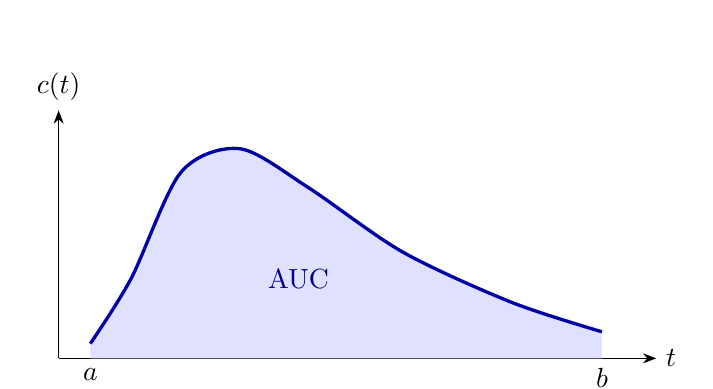
\begin{tikzpicture}[x=1.15cm,y=0.75cm,>=Stealth]
  \draw[->] (0,0) -- (6.6,0) node[right] {$t$};
  \draw[->] (0,0) -- (0,4.2) node[above] {$c(t)$};
  \fill[blue!12] (0.35,0)
    -- plot[smooth] coordinates {(0.35,0.25) (0.8,1.35) (1.35,3.15) (2.0,3.55) (2.75,2.9) (3.8,1.8) (5.0,0.95) (6.0,0.45)}
    -- (6.0,0) -- cycle;
  \draw[very thick,blue!65!black]
    plot[smooth] coordinates {(0.35,0.25) (0.8,1.35) (1.35,3.15) (2.0,3.55) (2.75,2.9) (3.8,1.8) (5.0,0.95) (6.0,0.45)};
  \node[blue!55!black] at (2.65,1.35) {AUC};
  \node[below] at (0.35,0) {$a$};
  \node[below] at (6.0,0) {$b$};
\end{tikzpicture}
\end{center}

从数学上看，浓度--时间曲线下方的面积就是一种\textbf{曲边梯形}的面积。为了说明这类面积怎样计算，设 $f(x)$ 是 $[a,b]$ 上的非负连续函数。由曲线 $y=f(x)$、直线 $x=a,x=b$ 与 $x$ 轴围成的图形称为曲边梯形。要求它的面积 $A$，在 $[a,b]$ 上任取一个分割
\[
a=x_0<x_1<\cdots<x_{n-1}<x_n=b.
\]
记
\[
\Delta x_i=x_i-x_{i-1},\qquad \lambda=\max_{1\leq i\leq n}\Delta x_i.
\]

\begin{center}
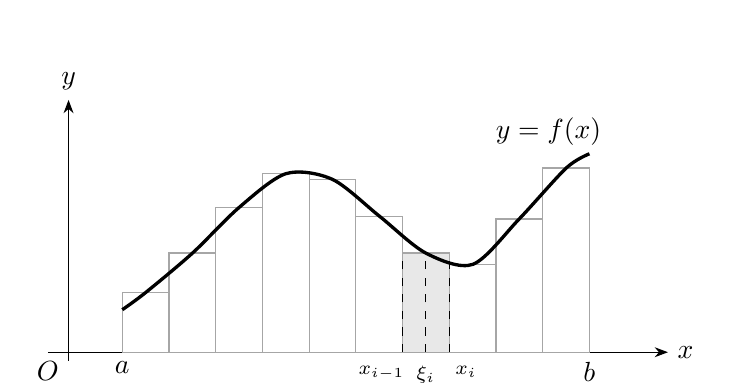
\begin{tikzpicture}[x=1.05cm,y=0.72cm,>=Stealth]
  \draw[->] (-0.25,0) -- (7.25,0) node[right] {$x$};
  \draw[->] (0,-0.15) -- (0,4.45) node[above] {$y$};
  \node[below left] at (0,0) {$O$};
  \def\a{0.65}
  \def\b{6.3}
  \def\xim{4.04}
  \def\xistar{4.32}
  \def\xip{4.605}
  \node[below] at (\a,0) {$a$};
  \node[below] at (\b,0) {$b$};
  \foreach \xl/\xr/\h in {
    0.65/1.215/1.05,
    1.215/1.78/1.75,
    1.78/2.345/2.55,
    2.345/2.91/3.15,
    2.91/3.475/3.05,
    3.475/4.04/2.40,
    4.04/4.605/1.75,
    4.605/5.17/1.55,
    5.17/5.735/2.35,
    5.735/6.3/3.25}
  {
    \draw[gray!70] (\xl,0) rectangle (\xr,\h);
  }
  \fill[gray!18] (\xim,0) rectangle (\xip,1.75);
  \draw[gray!70] (\xim,0) rectangle (\xip,1.75);
  \draw[very thick]
    plot[smooth] coordinates {(\a,0.75) (0.93,1.05) (1.50,1.75) (2.06,2.55) (2.63,3.15) (3.19,3.05) (3.76,2.40) (\xistar,1.75) (4.89,1.55) (5.45,2.35) (6.02,3.25) (\b,3.50)};
  \draw[dashed] (\xim,0) -- (\xim,1.75);
  \draw[dashed] (\xistar,0) -- (\xistar,1.75);
  \draw[dashed] (\xip,0) -- (\xip,1.75);
  \node[font=\scriptsize,anchor=north east] at (4.18,-0.08) {$x_{i-1}$};
  \node[font=\scriptsize,anchor=north] at (\xistar,-0.08) {$\xi_i$};
  \node[font=\scriptsize,anchor=north west] at (4.56,-0.08) {$x_i$};
  \node[above right] at (5.05,3.48) {$y=f(x)$};
\end{tikzpicture}
\end{center}

在第 $i$ 个小区间 $[x_{i-1},x_i]$ 中任取一点 $\xi_i$，用高为 $f(\xi_i)$、宽为 $\Delta x_i$ 的小矩形近似代替这一小段曲边梯形，则第 $i$ 小段的面积近似为
\[
f(\xi_i)\Delta x_i.
\]
于是总面积近似为
\[
A\approx \sum_{i=1}^n f(\xi_i)\Delta x_i.
\]
当 $\lambda$ 越来越小时，小矩形的近似误差越来越小，因此把曲边梯形面积定义为
\[
A=\lim_{\lambda\to0}\sum_{i=1}^n f(\xi_i)\Delta x_i.
\]
这给出了求曲边梯形面积的一般途径：分割、近似、求和、取极限。

\begin{custom}{路程问题}
设质点沿直线运动，时刻 $t$ 的速度为 $v(t)\geq0$，求它在 $[a,b]$ 内经过的路程 $s$。取分割
\[
a=t_0<t_1<\cdots<t_{n-1}<t_n=b,
\]
记
\[
\Delta t_i=t_i-t_{i-1},\qquad \lambda=\max_{1\leq i\leq n}\Delta t_i.
\]
如果速度是常数 $v_0$，路程就是 $v_0(b-a)$。现在速度随时间变化，但在很短的时间段 $[t_{i-1},t_i]$ 内，可以用某一点 $\xi_i$ 处的速度 $v(\xi_i)$ 近似代替这一小段内的速度。于是第 $i$ 小段路程近似为
\[
v(\xi_i)\Delta t_i,
\]
总路程近似为
\[
s\approx\sum_{i=1}^n v(\xi_i)\Delta t_i.
\]
令 $\lambda\to0$，得到
\[
s=\lim_{\lambda\to0}\sum_{i=1}^n v(\xi_i)\Delta t_i.
\]
由药物暴露量到曲边梯形面积，再到变速直线运动的路程，问题背景虽然不同，最后都落到同一类和式的极限。定积分正是为了统一处理这类连续累积问题而引入的。
\end{custom}

\subsection{定积分的概念}

前面两个例子背景不同，但最后都归结为同一类和式的极限。撇开各类问题的具体背景，把这种和式的极限抽象出来，就得到定积分的概念。

设函数 $f(x)$ 在区间 $[a,b]$ 上有界。任取分点
\[
a=x_0<x_1<\cdots<x_{n-1}<x_n=b,
\]
把 $[a,b]$ 分成 $n$ 个小区间 $[x_{i-1},x_i]$。记
\[
\Delta x_i=x_i-x_{i-1},\qquad \lambda=\max_{1\leq i\leq n}\Delta x_i.
\]
在每个小区间 $[x_{i-1},x_i]$ 中任取一点 $\xi_i$，作和式
\[
\sum_{i=1}^n f(\xi_i)\Delta x_i.
\]
这个和式称为函数 $f(x)$ 在 $[a,b]$ 上的一个\textbf{积分和}，也称为\textbf{黎曼和}。

\begin{definition}[定积分]
如果当 $\lambda\to0$ 时，积分和
\[
\sum_{i=1}^n f(\xi_i)\Delta x_i
\]
的极限存在，且这个极限与分法以及点 $\xi_i$ 的取法无关，则称函数 $f(x)$ 在 $[a,b]$ 上\textbf{可积}。这个极限称为 $f(x)$ 在 $[a,b]$ 上的\textbf{定积分}，记作
\[
\int_a^b f(x)\,\dd x
=\lim_{\lambda\to0}\sum_{i=1}^n f(\xi_i)\Delta x_i.
\]
其中 $f(x)$ 称为\textbf{被积函数}，$a$ 称为\textbf{积分下限}，$b$ 称为\textbf{积分上限}，$[a,b]$ 称为\textbf{积分区间}，$x$ 称为积分变量。
\end{definition}

定积分的值只与被积函数和积分区间有关，与积分变量的字母无关。因此
\[
\int_a^b f(x)\,\dd x=\int_a^b f(t)\,\dd t=\int_a^b f(u)\,\dd u.
\]
若 $f(x)$ 在 $[a,b]$ 上连续，则 $f(x)$ 在 $[a,b]$ 上可积（证明超出本讲义范围，从略）。更一般地，如果 $f(x)$ 在 $[a,b]$ 上有界，且只有有限个间断点，则它也可积。在本讲义中，若无特别说明，被积函数都取为连续函数或分段连续函数。


\begin{example}[用定义计算常数函数]
设 $k$ 为常数，计算
\[
\int_a^b k\,\dd x.
\]
对任意分割和任意取点 $\xi_i$，都有
\[
\sum_{i=1}^n k\Delta x_i
=k\sum_{i=1}^n \Delta x_i
=k(b-a).
\]
因此
\[
\int_a^b k\,\dd x=k(b-a).
\]
特别地，
\[
\int_a^b 1\,\dd x=b-a,
\]
这与长度的几何意义一致。
\end{example}

\noindent\textbf{定积分的几何意义}\quad 当 $f(x)\geq0$ 时，$\int_a^b f(x)\,\dd x$ 表示曲线 $y=f(x)$ 与 $x$ 轴、直线 $x=a,x=b$ 围成图形的面积。当 $f(x)$ 可正可负时，定积分表示带符号的面积：$x$ 轴上方的部分取正，$x$ 轴下方的部分取负。

\begin{example}[用定义计算]
计算
\[
\int_0^1 x^2\,\dd x.
\]
\begin{wrapfigure}{r}{0.28\textwidth}
\vspace{-1.2em}
\centering
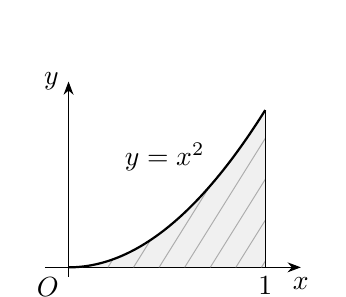
\begin{tikzpicture}[x=2.5cm,y=2.0cm,>=Stealth,baseline]
  \draw[->] (-0.12,0) -- (1.18,0) node[below] {$x$};
  \draw[->] (0,-0.06) -- (0,1.18) node[left] {$y$};
  \begin{scope}
    \clip (0,0) -- plot[domain=0:1,samples=60] (\x,{(\x)^2}) -- (1,0) -- cycle;
    \fill[gray!12] (0,0) rectangle (1,1);
    \foreach \s in {-0.45,-0.32,...,1.20}
      \draw[gray!65,line width=0.35pt] (\s,0) -- ({\s+0.55},1.1);
  \end{scope}
  \draw[thick,domain=0:1,samples=80] plot (\x,{(\x)^2});
  \draw (1,0) -- (1,1);
  \node[below left] at (0,0) {$O$};
  \node[below] at (1,0) {$1$};
  \node[above left] at (0.74,0.55) {$y=x^2$};
\end{tikzpicture}
\vspace{-1.2em}
\end{wrapfigure}
从几何意义看，这个定积分就是右图阴影部分的面积；下面仍按定义计算。
把 $[0,1]$ 等分成 $n$ 份，取右端点 $\xi_i=\frac{i}{n}$，则 $\Delta x=\frac1n$。于是
\[
\sum_{i=1}^n f(\xi_i)\Delta x
=\sum_{i=1}^n \left(\frac{i}{n}\right)^2\frac1n
=\frac1{n^3}\sum_{i=1}^n i^2.
\]
利用
\[
\sum_{i=1}^n i^2=\frac{n(n+1)(2n+1)}6,
\]
得
\[
\int_0^1 x^2\,\dd x
=\lim_{n\to\infty}\frac{n(n+1)(2n+1)}{6n^3}
=\frac13.
\]
\end{example}

从上面的例子可以看出，按定义计算定积分的基本步骤是“分割、近似、求和、取极限”
。定义可以直接计算一些简单定积分，但一般并不方便。实际计算定积分，主要依靠后面的微积分基本定理和各种积分法。
在建立更有效的计算方法之前，先列出定积分的一些基本性质。

\subsection{定积分的性质}

前面定义定积分时，一般假定积分下限小于积分上限，即 $a<b$。 为了使记号更加完整，约定
\[
\int_a^a f(x)\,\dd x=0,\qquad
\int_b^a f(x)\,\dd x=-\int_a^b f(x)\,\dd x.
\]
下面把定积分的常用性质分开列出。这些性质一方面来自定积分的定义，另一方面也是后面计算和估计定积分时经常使用的工具。

\begin{proposition}[线性性质]
设 $f(x),g(x)$ 在 $[a,b]$ 上可积，$k,l$ 为常数，则
\[
\int_a^b \bigl(kf(x)+lg(x)\bigr)\,\dd x
=k\int_a^b f(x)\,\dd x+l\int_a^b g(x)\,\dd x.
\]
\textbf{证明}\quad 对 $[a,b]$ 作任意分割，并在每个小区间上取点 $\xi_i$，则
\[
\sum_{i=1}^n\bigl(kf(\xi_i)+lg(\xi_i)\bigr)\Delta x_i
=k\sum_{i=1}^n f(\xi_i)\Delta x_i
+l\sum_{i=1}^n g(\xi_i)\Delta x_i.
\]
当分割加细并取极限时，左边趋于 $\int_a^b (kf(x)+lg(x))\,\dd x$，右边分别趋于 $k\int_a^b f(x)\,\dd x$ 与 $l\int_a^b g(x)\,\dd x$，所以结论成立。\hfill$\square$
\end{proposition}

\begin{proposition}[区间可加性]
设 $f(x)$ 在包含 $a,b,c$ 的区间上可积，且 $c$ 在 $a,b$ 之间，则
\[
\int_a^b f(x)\,\dd x=\int_a^c f(x)\,\dd x+\int_c^b f(x)\,\dd x.
\]
\textbf{证明}\quad 先设 $a<c<b$。 把 $[a,c]$ 和 $[c,b]$ 上的分割合并起来，就得到 $[a,b]$ 的一个分割。相应的积分和可写成两部分之和：
\[
\sum f(\xi_i)\Delta x_i
=\sum_{[a,c]} f(\xi_i)\Delta x_i+\sum_{[c,b]} f(\xi_i)\Delta x_i.
\]
两边分别取极限，便得
\[
\int_a^b f(x)\,\dd x=\int_a^c f(x)\,\dd x+\int_c^b f(x)\,\dd x.
\]
若 $c=a$ 或 $c=b$，结论由 $\int_a^a f(x)\,\dd x=0$ 得到。若积分上下限顺序改变，则由前面的约定同样成立。\hfill$\square$
\end{proposition}

\begin{proposition}[保号性与保序性]
若 $f(x)$ 在 $[a,b]$ 上可积，且 $f(x)\geq0$，则
\[
\int_a^b f(x)\,\dd x\geq0.
\]
若 $f(x),g(x)$ 在 $[a,b]$ 上可积，且 $f(x)\leq g(x)$，则
\[
\int_a^b f(x)\,\dd x\leq \int_a^b g(x)\,\dd x.
\]
\textbf{证明}\quad 若 $f(x)\geq0$，则每一个积分和
\[
\sum_{i=1}^n f(\xi_i)\Delta x_i
\]
都非负，取极限后仍非负，故 $\int_a^b f(x)\,\dd x\geq0$。若 $f(x)\leq g(x)$，则 $g(x)-f(x)\geq0$。由刚证得的保号性和线性性质，
\[
\int_a^b g(x)\,\dd x-\int_a^b f(x)\,\dd x
=\int_a^b (g(x)-f(x))\,\dd x\geq0,
\]
于是
\[
\int_a^b f(x)\,\dd x\leq \int_a^b g(x)\,\dd x.
\]
\noindent\hfill$\square$
\end{proposition}

\begin{proposition}[估值性质]
若 $f(x)$ 在 $[a,b]$ 上可积，且
\[
m\leq f(x)\leq M,\qquad a\leq x\leq b,
\]
则
\[
m(b-a)\leq \int_a^b f(x)\,\dd x\leq M(b-a).
\]
\textbf{证明}\quad 由保序性，有
\[
\int_a^b m\,\dd x\leq \int_a^b f(x)\,\dd x\leq \int_a^b M\,\dd x.
\]
又由常数函数的定积分公式，
\[
\int_a^b m\,\dd x=m(b-a),\qquad \int_a^b M\,\dd x=M(b-a),
\]
所以估值性质成立。\hfill$\square$
\end{proposition}

\begin{proposition}[绝对值不等式]
若 $f(x)$ 在 $[a,b]$ 上可积，则
\[
\left|\int_a^b f(x)\,\dd x\right|\leq \int_a^b |f(x)|\,\dd x.
\]
\textbf{证明}\quad 因为
\[
-|f(x)|\leq f(x)\leq |f(x)|,
\]
由保序性得
\[
-\int_a^b |f(x)|\,\dd x\leq \int_a^b f(x)\,\dd x\leq \int_a^b |f(x)|\,\dd x.
\]
这正是
\[
\left|\int_a^b f(x)\,\dd x\right|\leq \int_a^b |f(x)|\,\dd x.
\]
\noindent\hfill$\square$
\end{proposition}

估值性质和绝对值不等式常用于判断积分大小。在不能直接求出定积分时，先给出它的上下界也是一种重要方法。

\begin{theorem}[积分中值定理]
若 $f(x)$ 在 $[a,b]$ 上连续，且 $a<b$，则存在 $\xi\in[a,b]$，使得
\[
\int_a^b f(x)\,\dd x=f(\xi)(b-a).
\]
\textbf{证明}\quad 因为 $f(x)$ 在 $[a,b]$ 上连续，所以它在 $[a,b]$ 上能取到最大值和最小值。设
\[
m\leq f(x)\leq M,\qquad a\leq x\leq b.
\]
由估值性质，
\[
m(b-a)\leq \int_a^b f(x)\,\dd x\leq M(b-a).
\]
由于 $b-a>0$，两边同除以 $b-a$，得
\[
m\leq \frac1{b-a}\int_a^b f(x)\,\dd x\leq M.
\]
连续函数在区间上能取到介于最小值和最大值之间的任意值，因此存在 $\xi\in[a,b]$，使得
\[
f(\xi)=\frac1{b-a}\int_a^b f(x)\,\dd x.
\]
两边乘以 $b-a$，即得
\[
\int_a^b f(x)\,\dd x=f(\xi)(b-a).
\]
\noindent\hfill$\square$
\end{theorem}

积分中值定理可以理解为：连续函数在一段区间上的总累积量，等于某个中间值 $f(\xi)$ 乘以区间长度。因此
\[
\frac1{b-a}\int_a^b f(x)\,\dd x
\]
可看作 $f(x)$ 在 $[a,b]$ 上的平均值。

\begin{proposition}[奇偶性与周期性]
若 $f(x)$ 在 $[-a,a]$ 上可积，则
\[
\int_{-a}^{a} f(x)\,\dd x=0,\qquad f(x)\text{ 为奇函数},
\]
\[
\int_{-a}^{a} f(x)\,\dd x=2\int_0^a f(x)\,\dd x,\qquad f(x)\text{ 为偶函数}.
\]
若 \(f(x)\) 以 \(T>0\) 为周期且在任意有限区间上可积，则对任意实数 \(a\)，
\[
\int_a^{a+T} f(x)\,\dd x=\int_0^T f(x)\,\dd x.
\]
\textbf{证明}\quad 若 $f(x)$ 为奇函数，作代换 $x=-t$，则
\[
\int_{-a}^{0}f(x)\,\dd x
=\int_a^0 f(-t)(-\dd t)
=\int_0^a f(-t)\,\dd t
=-\int_0^a f(t)\,\dd t.
\]
所以 $\int_{-a}^{a}f(x)\,\dd x=0$。若 $f(x)$ 为偶函数，同理有
\[
\int_{-a}^{0}f(x)\,\dd x
=\int_0^a f(-t)\,\dd t
=\int_0^a f(t)\,\dd t,
\]
从而
\[
\int_{-a}^{a}f(x)\,\dd x=2\int_0^a f(x)\,\dd x.
\]
最后证明周期情形。由周期性可先把 \(a\) 改写为 \(a=mT+r\)，其中 \(m\) 为整数且 \(0\leq r<T\)；平移 \(mT\) 不改变函数值，故只需考虑 \(a=r\)。此时
\[
\begin{aligned}
\int_r^{r+T}f(x)\,\dd x
&=\int_r^T f(x)\,\dd x+\int_T^{T+r}f(x)\,\dd x\\
&=\int_r^T f(x)\,\dd x+\int_0^r f(u+T)\,\dd u\\
&=\int_r^T f(x)\,\dd x+\int_0^r f(u)\,\dd u\\
&=\int_0^T f(x)\,\dd x.
\end{aligned}
\]
\noindent\hfill$\square$
\end{proposition}

\begin{example}[利用奇偶性]
计算
\[
\int_{-1}^{1}(x^5+x^2)\,\dd x.
\]
其中 $x^5$ 为奇函数，$x^2$ 为偶函数，所以
\[
\int_{-1}^{1}(x^5+x^2)\,\dd x
=\int_{-1}^{1}x^5\,\dd x+\int_{-1}^{1}x^2\,\dd x
=2\int_0^1x^2\,\dd x=\frac23.
\]
\end{example}

\begin{example}[估计积分]
估计
\[
\int_0^1 \ee^{-x^2}\,\dd x
\]
的范围。

当 $0\leq x\leq1$ 时，$0\leq x^2\leq1$，所以
\[
\ee^{-1}\leq \ee^{-x^2}\leq1.
\]
由估值性质，
\[
\ee^{-1}\leq \int_0^1 \ee^{-x^2}\,\dd x\leq1.
\]
\end{example}

\begin{example}[利用周期性]
计算
\[
\int_0^{3\pi}|\sin x|\,\dd x.
\]
函数 $|\sin x|$ 的周期为 $\pi$，所以
\[
\int_0^{3\pi}|\sin x|\,\dd x
=3\int_0^\pi \sin x\,\dd x
=3\left[-\cos x\right]_0^\pi=6.
\]
\end{example}

\subsection{微积分基本定理}

在 2.1 节中按定义计算定积分，需要先求和式再取极限，即使被积函数很简单，计算也相当繁琐。自然要问：由极限定义的定积分，与由原函数定义的不定积分，这两个看似无关的概念之间是否有直接联系？微积分基本定理给出了肯定的回答，从而把定积分的计算化为求原函数。

\begin{definition}[积分上限函数]
设 $f(x)$ 在 $[a,b]$ 上连续。对 $x\in[a,b]$，定义
\[
\Phi(x)=\int_a^x f(t)\,\dd t,
\]
则称 $\Phi(x)$ 为 $f(x)$ 的\textbf{积分上限函数}。
\end{definition}

\begin{theorem}[积分上限函数的导数]
若 $f(x)$ 在 $[a,b]$ 上连续，则
\[
\Phi(x)=\int_a^x f(t)\,\dd t
\]
在 $(a,b)$ 内可导，且
\[
\Phi'(x)=f(x).
\]
\textbf{证明}\quad 对充分小的 $\Delta x$，有
\[
\Phi(x+\Delta x)-\Phi(x)=\int_x^{x+\Delta x}f(t)\,\dd t.
\]
由积分中值定理，存在 $\xi$ 介于 $x$ 与 $x+\Delta x$ 之间，使得
\[
\int_x^{x+\Delta x}f(t)\,\dd t=f(\xi)\Delta x.
\]
于是
\[
\frac{\Phi(x+\Delta x)-\Phi(x)}{\Delta x}=f(\xi).
\]
当 $\Delta x\to0$ 时，$\xi\to x$，由 $f$ 的连续性得 $\Phi'(x)=f(x)$。\hfill$\square$
\end{theorem}

\begin{example}[变上限积分求导]
求
\[
y=\int_1^{x^2}\ln(1+t^2)\,\dd t
\]
的导数。

令
\[
\Phi(u)=\int_1^u\ln(1+t^2)\,\dd t,
\]
则 $y=\Phi(x^2)$。由积分上限函数的导数和链式法则，
\[
y'=\Phi'(x^2)\cdot 2x=2x\ln(1+x^4).
\]
\end{example}

\begin{proposition}[变上下限积分求导]
设 $f(t)$ 连续，$u(x),v(x)$ 可导，则
\[
\left(\int_{v(x)}^{u(x)}f(t)\,\dd t\right)'
=f(u(x))u'(x)-f(v(x))v'(x).
\]
特别地，
\[
\left(\int_a^{u(x)}f(t)\,\dd t\right)'=f(u(x))u'(x),
\qquad
\left(\int_{v(x)}^b f(t)\,\dd t\right)'=-f(v(x))v'(x).
\]
\textbf{证明}\quad 令
\[
\Phi(y)=\int_a^y f(t)\,\dd t.
\]
则由积分上限函数的导数可知 $\Phi'(y)=f(y)$。又
\[
\int_{v(x)}^{u(x)}f(t)\,\dd t
=\int_a^{u(x)}f(t)\,\dd t-\int_a^{v(x)}f(t)\,\dd t
=\Phi(u(x))-\Phi(v(x)).
\]
两边对 $x$ 求导，并用链式法则，得
\[
\left(\int_{v(x)}^{u(x)}f(t)\,\dd t\right)'
=\Phi'(u(x))u'(x)-\Phi'(v(x))v'(x)
=f(u(x))u'(x)-f(v(x))v'(x).
\]
\noindent\hfill$\square$
\end{proposition}

\begin{example}[上下限都含 $x$]
求
\[
y=\int_x^{x^2} \ee^{-t^2}\,\dd t
\]
的导数。

由变上下限积分求导公式，取 $u(x)=x^2,\ v(x)=x$，得
\[
y'=\ee^{-(x^2)^2}\cdot 2x-\ee^{-x^2}\cdot 1
=2x \ee^{-x^4}-\ee^{-x^2}.
\]
也可以把积分拆成两个变上限积分：
\[
y=\int_0^{x^2}\ee^{-t^2}\,\dd t-\int_0^x \ee^{-t^2}\,\dd t,
\]
再分别求导，得到同样结果。遇到上下限都随 $x$ 改变的情形，先把它化为两个以常数为下限的积分，通常最不容易出错。
\end{example}

\noindent\textbf{补充（不作要求）}\quad 如果被积函数还含有参数 $x$，则求导时除了上下限变化带来的两项外，还要加上被积函数本身随 $x$ 变化产生的一项。具体地，若 $f(x,t)$ 关于 $x,t$ 有足够好的连续性，且关于 $x$ 的偏导数 $f_x(x,t)$ 连续，则
\[
\frac{\dd}{\dd x}\int_{v(x)}^{u(x)}f(x,t)\,\dd t
=f(x,u(x))u'(x)-f(x,v(x))v'(x)
+\int_{v(x)}^{u(x)}f_x(x,t)\,\dd t.
\]
当上下限为常数 $a,b$ 时，上式化为
\[
\frac{\dd}{\dd x}\int_a^b f(x,t)\,\dd t
=\int_a^b f_x(x,t)\,\dd t.
\]
这部分只作了解。下面回到定积分计算的基本公式。

\begin{theorem}[牛顿--莱布尼茨（Newton--Leibniz）公式]
若 $f(x)$ 在 $[a,b]$ 上连续，$F(x)$ 是 $f(x)$ 的一个原函数，则
\[
\int_a^b f(x)\,\dd x=F(b)-F(a).
\]
通常记作
\[
\int_a^b f(x)\,\dd x=\left.F(x)\right|_a^b.
\]
\textbf{证明}\quad 由上一定理，$\Phi(x)=\int_a^x f(t)\,\dd t$ 是 $f(x)$ 的一个原函数。若 $F(x)$ 也是 $f(x)$ 的原函数，则 $\Phi(x)=F(x)+C$。代入 $x=a$ 得 $\Phi(a)=0=F(a)+C$，所以 $C=-F(a)$。于是
\[
\int_a^b f(x)\,\dd x=\Phi(b)=F(b)-F(a).
\]
\noindent\hfill$\square$
\end{theorem}

\begin{example}[直接计算]
计算
\[
\int_0^1(3x^2+2x+1)\,\dd x.
\]
因为 $x^3+x^2+x$ 是 $3x^2+2x+1$ 的一个原函数，所以
\[
\int_0^1(3x^2+2x+1)\,\dd x
=\left.(x^3+x^2+x)\right|_0^1=3.
\]
\end{example}

\begin{example}[含绝对值的定积分]
计算
\[
\int_{-1}^{2}|x|\,\dd x.
\]
被积函数在 $x=0$ 处表达式发生变化，应先分段：
\[
|x|=
\begin{cases}
-x,&x<0,\\
x,&x\geq0.
\end{cases}
\]
于是
\[
\int_{-1}^{2}|x|\,\dd x
=\int_{-1}^0(-x)\,\dd x+\int_0^2x\,\dd x
=\frac12+2=\frac52.
\]
\end{example}

\begin{example}[分段后再用 牛顿--莱布尼茨公式]
计算
\[
\int_0^3 |x^2-1|\,\dd x.
\]
因为 $x^2-1$ 在 $[0,3]$ 内的零点为 $x=1$，所以
\[
|x^2-1|=
\begin{cases}
1-x^2,&0\leq x\leq1,\\
x^2-1,&1<x\leq3.
\end{cases}
\]
于是
\[
\begin{aligned}
\int_0^3 |x^2-1|\,\dd x
&=\int_0^1(1-x^2)\,\dd x+\int_1^3(x^2-1)\,\dd x\\
&=\left.\left(x-\frac{x^3}{3}\right)\right|_0^1
+\left.\left(\frac{x^3}{3}-x\right)\right|_1^3\\
&=\frac23+\frac{20}{3}=\frac{22}{3}.
\end{aligned}
\]
\end{example}

有些定积分虽然仍由 牛顿--莱布尼茨公式计算，但原函数不容易直接看出，这时需要把换元法和分部积分法用于定积分，并同时注意上下限和边界项。

\subsection{定积分的换元积分法与分部积分法}

定积分的换元法与不定积分的换元法一样，来源于复合函数求导法则。区别在于：定积分换元时，积分上下限也要随新变量一起改变。

\begin{theorem}[定积分的换元公式]
设 \(x=\varphi(t)\) 在 \([\alpha,\beta]\) 上有连续导数，且 \(\varphi(\alpha)=a,\ \varphi(\beta)=b\)。若 \(f\) 在包含 \(\varphi([\alpha,\beta])\) 的区间上连续，则
\[
\int_a^b f(x)\,\dd x
=\int_{\alpha}^{\beta}f(\varphi(t))\varphi'(t)\,\dd t.
\]
\end{theorem}

实际计算时，若令 $u=\varphi(x)$，则应同时把上下限换成
\[
x=a\Rightarrow u=\varphi(a),\qquad x=b\Rightarrow u=\varphi(b).
\]
这样计算结束后不必再代回原变量。

\begin{example}[换元后改变上下限]
计算
\[
\int_0^1 x\sqrt{1+x^2}\,\dd x.
\]
令 $u=1+x^2$，则 $\dd u=2x\,\dd x$。当 $x=0$ 时，$u=1$；当 $x=1$ 时，$u=2$。故
\[
\begin{aligned}
\int_0^1 x\sqrt{1+x^2}\,\dd x
&=\frac12\int_1^2 u^{1/2}\,\dd u\\
&=\frac12\left.\frac23u^{3/2}\right|_1^2
=\frac13(2\sqrt2-1).
\end{aligned}
\]
\end{example}

\begin{example}[半圆面积]
计算
\[
\int_{-a}^{a}\sqrt{a^2-x^2}\,\dd x\qquad(a>0).
\]
令 $x=a\sin t$，则 $\dd x=a\cos t\,\dd t$。当 $x=-a$ 时，$t=-\frac{\pi}{2}$；当 $x=a$ 时，$t=\frac{\pi}{2}$。于是
\[
\begin{aligned}
\int_{-a}^{a}\sqrt{a^2-x^2}\,\dd x
&=\int_{-\pi/2}^{\pi/2}a\cos t\cdot a\cos t\,\dd t\\
&=a^2\int_{-\pi/2}^{\pi/2}\cos^2t\,\dd t
=\frac{\pi a^2}{2}.
\end{aligned}
\]
这正是半径为 $a$ 的上半圆面积。
\end{example}

\begin{example}[对称性与换元结合]
计算
\[
\int_0^{\pi/2}\frac{\sin x}{\sin x+\cos x}\,\dd x.
\]
令
\[
I=\int_0^{\pi/2}\frac{\sin x}{\sin x+\cos x}\,\dd x.
\]
作代换 $x=\frac{\pi}{2}-t$，则
\[
I=\int_0^{\pi/2}\frac{\cos t}{\sin t+\cos t}\,\dd t.
\]
两式相加得
\[
2I=\int_0^{\pi/2}1\,\dd t=\frac{\pi}{2}.
\]
所以
\[
I=\frac{\pi}{4}.
\]
这类题不一定需要先求原函数，观察积分区间和被积函数的对称性往往更快。
\end{example}

\begin{theorem}[定积分的分部积分公式]
若 $u(x),v(x)$ 在 $[a,b]$ 上有连续导数，则
\[
\int_a^b u(x)v'(x)\,\dd x
=\left.u(x)v(x)\right|_a^b-\int_a^b v(x)u'(x)\,\dd x.
\]
也可写为
\[
\int_a^b u\,\dd v=\left.uv\right|_a^b-\int_a^b v\,\dd u.
\]
\textbf{证明}\quad 由乘积求导公式
\[
(uv)'=u'v+uv',
\]
两边在 $[a,b]$ 上积分，并用 牛顿--莱布尼茨公式，即得结论。\hfill$\square$
\end{theorem}

\begin{example}[对数函数]
计算
\[
\int_1^\ee\ln x\,\dd x.
\]
取 $u=\ln x,\ \dd v=\dd x$，则 $\dd u=\frac1x\dd x,\ v=x$。故
\[
\int_1^\ee\ln x\,\dd x
=\left.x\ln x\right|_1^\ee-\int_1^\ee1\,\dd x
=\ee-(\ee-1)=1.
\]
\end{example}

\begin{example}[含参数的递推型]
设
\[
I_n=\int_0^{\pi/2}\sin^n x\,\dd x\qquad(n\geq2).
\]
因为
\[
I_n=\int_0^{\pi/2}\sin^{n-1}x\sin x\,\dd x,
\]
取 $u=\sin^{n-1}x,\ \dd v=\sin x\,\dd x$，则 $v=-\cos x$。分部积分得
\[
\begin{aligned}
I_n
&=\left.-\sin^{n-1}x\cos x\right|_0^{\pi/2}
+(n-1)\int_0^{\pi/2}\sin^{n-2}x\cos^2x\,\dd x\\
&=(n-1)\int_0^{\pi/2}\sin^{n-2}x(1-\sin^2x)\,\dd x\\
&=(n-1)(I_{n-2}-I_n).
\end{aligned}
\]
因此
\[
I_n=\frac{n-1}{n}I_{n-2}.
\]
\end{example}

\begin{example}[连续两次分部积分]
计算
\[
\int_0^\pi \ee^x\sin x\,\dd x.
\]
记
\[
I=\int_0^\pi \ee^x\sin x\,\dd x.
\]
先取 $u=\sin x,\ \dd v=\ee^x\dd x$，得
\[
I=\left.\ee^x\sin x\right|_0^\pi-\int_0^\pi \ee^x\cos x\,\dd x
=-\int_0^\pi \ee^x\cos x\,\dd x.
\]
再对右端积分分部积分：
\[
\int_0^\pi \ee^x\cos x\,\dd x
=\left.\ee^x\cos x\right|_0^\pi+\int_0^\pi \ee^x\sin x\,\dd x
=-\ee^\pi-1+I.
\]
于是
\[
I=-(-\ee^\pi-1+I),
\]
所以
\[
\int_0^\pi \ee^x\sin x\,\dd x=\frac{\ee^\pi+1}{2}.
\]
\end{example}

\begin{custom}{定积分的计算思路}
计算定积分时，一般按以下顺序观察：
\begin{enumerate}
\item 先看区间和被积函数是否有奇偶性、周期性或对称性；
\item 再看是否能直接找到原函数，用 牛顿--莱布尼茨公式计算；
\item 若被积函数含复合结构，考虑换元，并同时改变上下限；
\item 若被积函数是乘积，特别是含有 $\ln x$、反三角函数、多项式乘指数函数或三角函数，考虑分部积分；
\item 若被积函数含绝对值或分段表达式，先分段，再分别积分。
\end{enumerate}
定积分的结果是一个数。换元后上下限已经改变时，计算结束不必再代回原变量；分部积分时，边界项 $\left.uv\right|_a^b$ 不能漏掉。
\end{custom}

\subsection{定积分的应用}

定积分应用的基本思想是\textbf{微元法}：先在一个很小的区间上写出局部近似量，再把这些局部近似量累加，最后取极限。写成公式时，就是把微元 $\dd x$ 或 $\dd t$ 上的近似量积分起来。

使用微元法时，可按以下步骤进行：
\begin{enumerate}
\item 选定积分变量，并确定它的变化区间；
\item 在一个小区间上写出局部量的近似表达式；
\item 把局部量写成形如 $q(x)\dd x$ 的微元；
\item 在整个区间上积分。
\end{enumerate}
关键是第二步：小区间足够短时，连续变化的量可以近似看成常量，曲边小块可以近似看成规则图形。这正是定积分定义中“局部近似，再求和取极限”的思想。

\begin{custom}{平面图形面积}
平面图形面积的基本原则是“上减下”或“右减左”。若在 $[a,b]$ 上有 $f(x)\geq g(x)$，则两条曲线 $y=f(x)$ 与 $y=g(x)$ 之间的面积为
\[
S=\int_a^b\bigl(f(x)-g(x)\bigr)\,\dd x.
\]
若用 $y$ 作积分变量，且在 $[c,d]$ 上右边界为 $x=\varphi(y)$，左边界为 $x=\psi(y)$，则
\[
S=\int_c^d\bigl(\varphi(y)-\psi(y)\bigr)\,\dd y.
\]
选用 $x$ 还是 $y$ 作积分变量，主要看哪一方向上的上下边界或左右边界更容易写出。如果两条曲线的上下关系发生改变，应先按交点把区域分段。
\end{custom}

\begin{example}[两曲线围成面积]
求曲线 $y=x$ 与 $y=x^2$ 围成图形的面积。

交点由 $x=x^2$ 得 $x=0,1$。在 $[0,1]$ 上有 $x\geq x^2$，所以
\[
S=\int_0^1(x-x^2)\,\dd x
=\left.\left(\frac{x^2}{2}-\frac{x^3}{3}\right)\right|_0^1
=\frac16.
\]
\end{example}

\begin{example}[用 $y$ 作积分变量]
求曲线 $x=y^2$ 与直线 $x=2-y$ 围成图形的面积。

交点由
\[
y^2=2-y
\]
得 $y=-2,1$。在 $[-2,1]$ 上，右边界为 $x=2-y$，左边界为 $x=y^2$。所以
\[
\begin{aligned}
S&=\int_{-2}^1\bigl[(2-y)-y^2\bigr]\,\dd y\\
&=\left.\left(2y-\frac{y^2}{2}-\frac{y^3}{3}\right)\right|_{-2}^{1}
=\frac92.
\end{aligned}
\]
当图形左右边界比较清楚时，用 $y$ 作积分变量往往比解出上下边界更简洁。
\end{example}

\begin{custom}{已知平行截面的立体体积}
如果一个立体被一族互相平行的平面截开，并且垂直于 $x$ 轴、过点 $x$ 的截面面积为 $A(x)$，其中 $a\leq x\leq b$，则该立体的体积为
\[
V=\int_a^b A(x)\,\dd x.
\]
这是面积公式的空间版本。在 $[x,x+\dd x]$ 上取一薄片，当 $\dd x$ 很小时，这一薄片的体积近似为
\[
\dd V=A(x)\,\dd x.
\]
若垂直于 $y$ 轴的截面面积为 $B(y)$，其中 $c\leq y\leq d$，则同理有
\[
V=\int_c^d B(y)\,\dd y.
\]
\end{custom}

\begin{example}[已知截面积求体积]
某立体垂直于 $x$ 轴的截面都是正方形，且在位置 $x$ 处正方形的边长为 $\sqrt{1+x}$，其中 $0\leq x\leq3$。求该立体的体积。

截面面积为
\[
A(x)=(\sqrt{1+x})^2=1+x.
\]
故体积为
\[
V=\int_0^3(1+x)\,\dd x
=\left.\left(x+\frac{x^2}{2}\right)\right|_0^3
=\frac{15}{2}.
\]
\end{example}

\begin{custom}{旋转体的体积}
旋转体体积可以看作截面法的特殊情形。若曲线 $y=f(x)\geq0$、直线 $x=a,x=b$ 与 $x$ 轴围成的曲边梯形绕 $x$ 轴旋转一周，则在位置 $x$ 处的截面是半径为 $f(x)$ 的圆，所以
\[
V=\pi\int_a^b [f(x)]^2\,\dd x.
\]
更一般地，若 $0\leq g(x)\leq f(x)$，两条曲线 $y=f(x),y=g(x)$ 之间的图形绕 $x$ 轴旋转一周，则截面为圆环，外半径为 $f(x)$，内半径为 $g(x)$，因此
\[
V=\pi\int_a^b\bigl([f(x)]^2-[g(x)]^2\bigr)\,\dd x.
\]
若用 $y$ 作积分变量，例如图形绕 $y$ 轴旋转，则把横向半径写成 $y$ 的函数。若 $x=\varphi(y)\geq0$，$c\leq y\leq d$，则
\[
V=\pi\int_c^d [\varphi(y)]^2\,\dd y.
\]
\end{custom}

\begin{example}[绕 $x$ 轴旋转]
求由 $y=x^2$、$x=0$、$x=1$ 与 $x$ 轴围成的曲边梯形绕 $x$ 轴旋转一周所得旋转体的体积。

在位置 $x$ 处，截面是半径为 $x^2$ 的圆，截面面积为
\[
A(x)=\pi x^4.
\]
因此
\[
V=\pi\int_0^1x^4\,\dd x=\frac{\pi}{5}.
\]
\end{example}

\begin{example}[绕 $y$ 轴旋转]
求由 $y=x^2$、$y=1$ 与 $y$ 轴围成的图形绕 $y$ 轴旋转一周所得旋转体的体积。

用 $y$ 作积分变量。由 $y=x^2$ 得 $x=\sqrt y$，且 $0\leq y\leq1$。绕 $y$ 轴旋转时，位置 $y$ 处的截面是半径为 $\sqrt y$ 的圆，故
\[
V=\pi\int_0^1(\sqrt y)^2\,\dd y
=\pi\int_0^1y\,\dd y
=\frac{\pi}{2}.
\]
\end{example}

\begin{custom}{变化率与总量}
如果某个量 $Q(t)$ 的变化率为 $q(t)$，则从 $t=a$ 到 $t=b$ 的改变量等于变化率在这段区间上的累积：
\[
\Delta Q=Q(b)-Q(a)=\int_a^b q(t)\,\dd t.
\]
这类问题常见于总产量、总成本、总收益、人口变化、温度变化等连续累积模型。题目若给出“每单位时间的变化量”，通常就应考虑把变化率积分起来。
\end{custom}

\begin{example}[由变化率求总量]
某量 $Q(t)$ 的变化率为
\[
Q'(t)=3t^2+2t,\qquad 0\leq t\leq2.
\]
求这段时间内 $Q$ 的改变量。

由定积分的意义，
\[
\Delta Q=Q(2)-Q(0)=\int_0^2(3t^2+2t)\,\dd t
=\left.(t^3+t^2)\right|_0^2=12.
\]
\end{example}

\begin{custom}{运动学应用：由速度求路程}
若质点沿直线运动，速度为 $v(t)$。当 $v(t)\geq0$ 时，从 $t=a$ 到 $t=b$ 经过的路程为
\[
s=\int_a^b v(t)\,\dd t.
\]
若速度可能取负，则位移为
\[
\Delta x=\int_a^b v(t)\,\dd t,
\]
路程应计算
\[
s=\int_a^b |v(t)|\,\dd t.
\]
\end{custom}

\begin{example}[由速度求路程]
某质点作直线运动，速度为
\[
v(t)=2t+1,\qquad 0\leq t\leq3.
\]
求这段时间内质点经过的路程。

由于 $v(t)>0$，所以路程为
\[
s=\int_0^3(2t+1)\,\dd t
=\left.(t^2+t)\right|_0^3=12.
\]
\end{example}

\begin{custom}{物理应用：变力做功}
若物体沿直线从 $x=a$ 移动到 $x=b$，受力 $F(x)$ 与位置有关，且方向与运动方向一致，则在小位移 $\dd x$ 上所做的功近似为
\[
\dd W=F(x)\,\dd x.
\]
因此总功为
\[
W=\int_a^bF(x)\,\dd x.
\]
如果力的方向与运动方向相反，积分结果会带负号；在只求功的大小时，要根据题意处理符号。
\end{custom}

\begin{example}[变力做功]
某物体沿直线运动，所受力为
\[
F(x)=2x+1.
\]
求物体从 $x=0$ 移动到 $x=3$ 时该力所做的功。

\[
W=\int_0^3(2x+1)\,\dd x=\left.(x^2+x)\right|_0^3=12.
\]
\end{example}

\begin{application}[农业：总灌溉水量]
设灌溉系统从启动到稳定的流量用简化模型
\[
q(t)=q_0(1-\ee^{-kt}),\qquad q_0>0,\quad k>0
\]
描述，其中 $t$ 的单位为 $\mathrm h$，$q$ 的单位为 $\mathrm{m^3/h}$。假设参数在 $0\leq t\leq T$ 内保持不变，则总供水量为
\[
\begin{aligned}
W&=\int_0^Tq(t)\,\dd t\\
&=q_0\int_0^T(1-\ee^{-kt})\,\dd t
=q_0\left[T-\frac{1-\ee^{-kT}}{k}\right].
\end{aligned}
\]
因此 $[W]=\mathrm{m^3}$。式中的第二项反映启动阶段尚未达到稳定流量所造成的供水量差额。实际系统还会受压力波动、阀门控制、渗漏和流量计误差影响，本例只说明“流量的定积分等于累计水量”。
\end{application}

\begin{custom}{应用题的共同结构}
定积分应用题看起来类型很多，核心都可以归结为“总量等于局部量的累积”。面积问题中，局部量是小矩形面积；已知截面的体积问题中，局部量是薄片体积；旋转体问题中，局部量是圆片或圆环体积；变化率、路程和做功问题中，局部量分别是小段改变量、小段路程和小段功。写公式前先问一句：在一个很小的区间上，这一小段贡献是多少？能写出这个微元，积分式通常就确定了。
\end{custom}

\subsection{反常积分初步}

前面讨论的定积分有两个基本前提：积分区间是有限闭区间，被积函数在这个区间上有界。如果积分区间无限，或者被积函数在积分区间的某一点附近无界，就不能直接照搬通常的定积分定义。这时引入\textbf{反常积分}。反常积分的思想仍然是极限：先在没有问题的有限区间上作普通定积分，再让端点趋向无穷远处，或让端点趋向无界点。

学习反常积分时要先分清两个问题：第一，积分是否\textbf{收敛}；第二，如果收敛，它的值是多少。若对应的极限不存在，或趋于无穷大，就称反常积分\textbf{发散}。许多题目只要求判断收敛性，此时不一定要把积分值算出来。

\begin{definition}[无穷区间上的反常积分]
若 $f(x)$ 在 $[a,+\infty)$ 上连续，则定义
\[
\int_a^{+\infty}f(x)\,\dd x
=\lim_{A\to+\infty}\int_a^A f(x)\,\dd x.
\]
若右端极限存在，则称该反常积分\textbf{收敛}；若极限不存在，则称其\textbf{发散}。

类似地，若 $f(x)$ 在 $(-\infty,b]$ 上连续，则
\[
\int_{-\infty}^b f(x)\,\dd x
=\lim_{A\to-\infty}\int_A^b f(x)\,\dd x.
\]
若 $f(x)$ 在 $(-\infty,+\infty)$ 上连续，则先任取一点 $c$，把积分分成
\[
\int_{-\infty}^{+\infty}f(x)\,\dd x
=\int_{-\infty}^{c}f(x)\,\dd x+\int_c^{+\infty}f(x)\,\dd x.
\]
只有右边两个反常积分都收敛时，才称左边的积分收敛。
\end{definition}

\begin{example}[指数函数在无穷区间上的积分]
讨论
\[
\int_0^{+\infty}\ee^{-ax}\,\dd x
\]
的收敛性，其中 $a$ 为常数。

若 $a>0$，则
\[
\int_0^A \ee^{-ax}\,\dd x
=\left.-\frac1a \ee^{-ax}\right|_0^A
=\frac{1-\ee^{-aA}}a.
\]
令 $A\to+\infty$，得
\[
\int_0^{+\infty}\ee^{-ax}\,\dd x=\frac1a.
\]
若 $a=0$，则被积函数恒为 $1$，积分发散；若 $a<0$，则 $\ee^{-ax}$ 随 $x$ 增大而增大，积分也发散。因此
\[
\int_0^{+\infty}\ee^{-ax}\,\dd x
\begin{cases}
\text{收敛,且等于 }\dfrac1a,&a>0,\\
\text{发散},&a\leq0.
\end{cases}
\]
\end{example}

\begin{example}[$p$ 型无穷积分]
讨论
\[
\int_1^{+\infty}\frac1{x^p}\,\dd x
\]
的收敛性，其中 $p$ 为常数。

当 $p\neq1$ 时，
\[
\int_1^A x^{-p}\,\dd x
=\left.\frac{x^{1-p}}{1-p}\right|_1^A
=\frac{A^{1-p}-1}{1-p}.
\]
若 $p>1$，则 $A^{1-p}\to0$，积分收敛，且
\[
\int_1^{+\infty}\frac1{x^p}\,\dd x=\frac1{p-1}.
\]
若 $p<1$，则极限不存在，积分发散。当 $p=1$ 时，
\[
\int_1^A\frac1x\,\dd x=\ln A\to+\infty,
\]
也发散。因此
\[
\int_1^{+\infty}\frac1{x^p}\,\dd x
\begin{cases}
\text{收敛},&p>1,\\
\text{发散},&p\leq1.
\end{cases}
\]
\end{example}

\begin{custom}{无穷区间上的基本判断}
上例是最常用的比较对象之一。在 $[1,+\infty)$ 上，
\[
\int_1^{+\infty}\frac1{x^p}\,\dd x
\]
当 $p>1$ 时收敛，当 $p\leq1$ 时发散。直观上说，函数在无穷远处下降得足够快，曲线下面积才可能有限。很多题只需把被积函数在 $+\infty$ 附近与 $\frac1{x^p}$ 比较。
\end{custom}

\begin{definition}[无界函数的反常积分]
若 $f(x)$ 在 $(a,b]$ 上连续，且在 $x=a$ 的右侧无界，则定义
\[
\int_a^b f(x)\,\dd x
=\lim_{\varepsilon\to0^+}\int_{a+\varepsilon}^b f(x)\,\dd x.
\]
若右端极限存在，则称该反常积分收敛；否则称其发散。

若 $f(x)$ 在 $[a,b)$ 上连续，且在 $x=b$ 的左侧无界，则定义
\[
\int_a^b f(x)\,\dd x
=\lim_{\varepsilon\to0^+}\int_a^{b-\varepsilon} f(x)\,\dd x.
\]
若无界点 $c$ 在区间内部，则应分成两部分：
\[
\int_a^b f(x)\,\dd x
=\int_a^c f(x)\,\dd x+\int_c^b f(x)\,\dd x.
\]
只有这两个反常积分都收敛时，原积分才收敛。这样的无界点也称为\textbf{瑕点}。
\end{definition}

\begin{example}[$p$ 型瑕积分]
讨论
\[
\int_0^1\frac1{x^p}\,\dd x
\]
的收敛性。

当 $p\neq1$ 时，
\[
\int_\varepsilon^1x^{-p}\,\dd x
=\left.\frac{x^{1-p}}{1-p}\right|_{\varepsilon}^{1}
=\frac{1-\varepsilon^{1-p}}{1-p}.
\]
若 $p<1$，则 $\varepsilon^{1-p}\to0$，积分收敛，且
\[
\int_0^1\frac1{x^p}\,\dd x=\frac1{1-p}.
\]
若 $p>1$，则极限不存在，积分发散。当 $p=1$ 时，
\[
\int_\varepsilon^1\frac1x\,\dd x=-\ln\varepsilon\to+\infty,
\]
也发散。因此
\[
\int_0^1\frac1{x^p}\,\dd x
\begin{cases}
\text{收敛},&p<1,\\
\text{发散},&p\geq1.
\end{cases}
\]
\end{example}

\begin{custom}{无界点附近的基本判断}
在 $(0,1]$ 上，
\[
\int_0^1\frac1{x^p}\,\dd x
\]
当 $p<1$ 时收敛，当 $p\geq1$ 时发散。这与无穷区间上的结论方向相反：在 $0$ 附近，$\frac1{x^p}$ 爆得太快时，面积会变成无穷大。
\end{custom}

\begin{example}[端点无界但积分收敛]
计算
\[
\int_0^1\frac{x^3}{\sqrt{1-x^2}}\,\dd x.
\]
被积函数在 $x=1$ 附近无界，因此这是反常积分。按定义，
\[
\int_0^1\frac{x^3}{\sqrt{1-x^2}}\,\dd x
=\lim_{\varepsilon\to0^+}\int_0^{1-\varepsilon}\frac{x^3}{\sqrt{1-x^2}}\,\dd x.
\]
令 $u=1-x^2$，则 $x\,\dd x=-\frac12\dd u$，且 $x^2=1-u$。于是
\[
\int_0^{1-\varepsilon}\frac{x^3}{\sqrt{1-x^2}}\,\dd x
=\frac12\int_{2\varepsilon-\varepsilon^2}^{1}(1-u)u^{-\frac12}\,\dd u.
\]
令 $\varepsilon\to0^+$，得
\[
\int_0^1\frac{x^3}{\sqrt{1-x^2}}\,\dd x
=\frac12\int_0^1(1-u)u^{-\frac12}\,\dd u
=\frac12\left(2-\frac23\right)=\frac23.
\]
这个例子说明，反常积分在作适当变量代换以后，有时会化成更容易计算的反常积分；上式右端在 \(u=0\) 处仍是反常的。
\end{example}

\begin{example}[内部瑕点必须拆开]
讨论
\[
\int_{-1}^1\frac1{x^2}\,\dd x
\]
的收敛性。

被积函数在 $x=0$ 处无界，所以要拆成
\[
\int_{-1}^1\frac1{x^2}\,\dd x
=\int_{-1}^0\frac1{x^2}\,\dd x+\int_0^1\frac1{x^2}\,\dd x.
\]
其中
\[
\int_0^1\frac1{x^2}\,\dd x
=\lim_{\varepsilon\to0^+}\int_{\varepsilon}^1\frac1{x^2}\,\dd x
=\lim_{\varepsilon\to0^+}\left(-1+\frac1{\varepsilon}\right)=+\infty.
\]
因此原反常积分发散。

这里不能直接写
\[
\int_{-1}^1\frac1{x^2}\,\dd x
=\left.-\frac1x\right|_{-1}^{1}=-2.
\]
牛顿--莱布尼茨公式要求被积函数在闭区间上连续，且原函数在整个区间上有效；这里 $x=0$ 是瑕点，上面的做法漏掉了反常积分的定义。
\end{example}

\begin{theorem}[比较判别法]
设 $f(x),g(x)$ 在 $[a,+\infty)$ 上非负连续，且当 $x$ 充分大时有
\[
0\leq f(x)\leq g(x).
\]
如果
\[
\int_a^{+\infty}g(x)\,\dd x
\]
收敛，则
\[
\int_a^{+\infty}f(x)\,\dd x
\]
也收敛；如果
\[
\int_a^{+\infty}f(x)\,\dd x
\]
发散，则
\[
\int_a^{+\infty}g(x)\,\dd x
\]
也发散。

无界函数的反常积分也有同样的比较思想，只需把“$x$ 充分大”换成“在瑕点附近”。
\end{theorem}

\begin{example}[用比较判别法判断收敛]
讨论
\[
\int_1^{+\infty}\frac{\ln x}{x^2}\,\dd x
\]
的收敛性。

当 $x$ 充分大时，$\ln x<\sqrt{x}$，于是
\[
0\leq\frac{\ln x}{x^2}<\frac{\sqrt{x}}{x^2}=\frac1{x^{3/2}}.
\]
而
\[
\int_1^{+\infty}\frac1{x^{3/2}}\,\dd x
\]
收敛，所以由比较判别法可知
\[
\int_1^{+\infty}\frac{\ln x}{x^2}\,\dd x
\]
收敛。

事实上，这个积分也可以直接用分部积分计算：
\[
\int_1^A\frac{\ln x}{x^2}\,\dd x
=\left.-\frac{\ln x}{x}\right|_1^A+\int_1^A\frac1{x^2}\,\dd x
=-\frac{\ln A}{A}+1-\frac1A.
\]
令 $A\to+\infty$，得
\[
\int_1^{+\infty}\frac{\ln x}{x^2}\,\dd x=1.
\]
\end{example}

\begin{example}[无界点附近的比较]
讨论
\[
\int_0^1\frac{\sin\frac1x}{\sqrt{x}}\,\dd x
\]
的收敛性。

因为
\[
\left|\frac{\sin\frac1x}{\sqrt{x}}\right|\leq\frac1{\sqrt{x}},
\]
且
\[
\int_0^1\frac1{\sqrt{x}}\,\dd x
\]
收敛，所以
\[
\int_0^1\left|\frac{\sin\frac1x}{\sqrt{x}}\right|\,\dd x
\]
收敛。这时称原反常积分\textbf{绝对收敛}。绝对收敛一定推出收敛，因此原反常积分收敛。
\end{example}

\begin{custom}{$\Gamma$ 函数与 $\mathrm B$ 函数简介}
有些重要函数本身就是由反常积分定义的。其中最常见的是 \textbf{$\Gamma$ 函数}。对 $a>0$，定义
\[
\Gamma(a)=\int_0^{+\infty}x^{a-1}\ee^{-x}\,\dd x.
\]
这个积分有两个需要注意的地方：一是积分区间为 $[0,+\infty)$，二是当 $0<a<1$ 时，$x^{a-1}$ 在 $x=0$ 附近无界。因此它是一个典型的反常积分。它的收敛性可分两段看：
\[
\int_0^{+\infty}x^{a-1}\ee^{-x}\,\dd x
=\int_0^1x^{a-1}\ee^{-x}\,\dd x+\int_1^{+\infty}x^{a-1}\ee^{-x}\,\dd x.
\]
在 $(0,1]$ 上，$\ee^{-x}$ 有界且接近 $1$，所以收敛性与
\[
\int_0^1x^{a-1}\,\dd x
\]
相同，故要求 $a>0$。在 $[1,+\infty)$ 上，指数函数 $\ee^{-x}$ 衰减很快，足以保证积分收敛。因此 $\Gamma(a)$ 在 $a>0$ 时有定义。

$\Gamma$ 函数满足一个重要递推公式：
\[
\Gamma(a+1)=a\Gamma(a)\qquad(a>0).
\]
这是由分部积分得到的。事实上，先在有限区间 $[\varepsilon,A]$ 上分部积分，再令 $\varepsilon\to0^+,\ A\to+\infty$，即可得到上式。特别地，
\[
\Gamma(1)=\int_0^{+\infty}\ee^{-x}\,\dd x=1,
\]
于是对正整数 $n$，有
\[
\Gamma(n+1)=n!.
\]

另一个常见函数是 \textbf{$\mathrm B$ 函数}。对 $p>0,\ q>0$，定义
\[
\mathrm B(p,q)=\int_0^1x^{p-1}(1-x)^{q-1}\,\dd x.
\]
这个积分在两个端点都可能出现无界情形：$x=0$ 附近主要看 $x^{p-1}$，$x=1$ 附近主要看 $(1-x)^{q-1}$，因此 $p>0,\ q>0$ 时收敛。由代换 $x=1-t$ 可知
\[
\mathrm B(p,q)=\mathrm B(q,p).
\]
此外，$\Gamma$ 函数与 $\mathrm B$ 函数之间有联系公式
\[
\mathrm B(p,q)=\frac{\Gamma(p)\Gamma(q)}{\Gamma(p+q)}\qquad(p>0,\ q>0),
\]
本讲义只作介绍，不要求证明。
\end{custom}

\begin{example}[Gamma 函数的简单计算]
计算 $\Gamma(4)$。

由递推公式，
\[
\Gamma(4)=3\Gamma(3)=3\cdot2\Gamma(2)=3\cdot2\cdot1\Gamma(1)=3!=6.
\]
也就是说，
\[
\int_0^{+\infty}x^3\ee^{-x}\,\dd x=6.
\]
\end{example}

\begin{example}[Beta 函数的简单计算]
计算 $\mathrm B(2,3)$。

按定义，
\[
\mathrm B(2,3)=\int_0^1x(1-x)^2\,\dd x
=\int_0^1(x-2x^2+x^3)\,\dd x.
\]
因此
\[
\mathrm B(2,3)=\left.\left(\frac{x^2}{2}-\frac{2x^3}{3}+\frac{x^4}{4}\right)\right|_0^1
=\frac12-\frac23+\frac14=\frac1{12}.
\]
\end{example}

\begin{custom}{关于柯西主值的提醒}
有些对称极限会给出一个有限值，称为\textbf{柯西主值}。例如
\[
\lim_{\varepsilon\to0^+}\left(\int_{-1}^{-\varepsilon}\frac1x\,\dd x+\int_{\varepsilon}^{1}\frac1x\,\dd x\right)=0.
\]
但
\[
\int_{-1}^{0}\frac1x\,\dd x,\qquad \int_{0}^{1}\frac1x\,\dd x
\]
分别发散，所以
\[
\int_{-1}^{1}\frac1x\,\dd x
\]
作为反常积分是发散的。本节只把柯西主值作为提醒：遇到内部瑕点时，必须按定义分别讨论左右两边，不能用对称抵消代替收敛性判断。
\end{custom}

\begin{custom}{反常积分的计算步骤}
计算反常积分时，一般按下面几步做：
\begin{enumerate}
\item 找出导致反常的地方：无穷区间、端点无界、内部瑕点，或几种情况同时出现；
\item 把积分拆成若干个只含一个反常点的积分；
\item 对每一部分写成普通定积分的极限；
\item 先判断极限是否存在；若存在，再求积分值；
\item 只要有一部分发散，原反常积分就发散。
\end{enumerate}
在实际计算中，若原函数容易求，就直接按定义取极限；若原函数不容易求，常用 $p$ 型积分、指数衰减和比较判别法先判断收敛性。
\end{custom}

\subsection{二重积分的概念与计算}

一元定积分处理区间上的累积量，二重积分则把“分割、近似、求和、取极限”的思想推广到平面区域。下面从曲顶柱体的体积出发建立二重积分，并介绍直角坐标与极坐标下的计算方法。

\textbf{曲顶柱体的体积}

设 $D$ 是 $xOy$ 平面上的有界闭区域，函数 $f(x,y)$ 在 $D$ 上连续且满足 $f(x,y)\geq0$。以 $D$ 为底，曲面 $z=f(x,y)$ 为顶，并以平行于 $z$ 轴的直线为侧棱，得到一个曲顶柱体。当 $f(x,y)$ 不是常数时，这个立体的高度随底面位置变化，不能直接使用“底面积乘高”得到体积。

把底面区域 $D$ 分成 $n$ 个小区域 $\Delta D_1,\Delta D_2,\ldots,\Delta D_n$，记它们的面积为 $\Delta\sigma_1,\Delta\sigma_2,\ldots,\Delta\sigma_n$。在每个小区域 $\Delta D_i$ 内取一点 $(\xi_i,\eta_i)$。当分割足够细时，曲顶柱体在 $\Delta D_i$ 上方的那一小块可以近似看成高为 $f(\xi_i,\eta_i)$ 的小柱体，于是
\[
\Delta V_i\approx f(\xi_i,\eta_i)\Delta\sigma_i.
\]
把所有小块的体积近似值相加，得到
\[
V\approx\sum_{i=1}^n f(\xi_i,\eta_i)\Delta\sigma_i.
\]
令各小区域的直径中的最大值趋于 $0$，上式的近似值趋于曲顶柱体的准确体积，因而
\[
V=\lim_{\lambda\to0}\sum_{i=1}^n f(\xi_i,\eta_i)\Delta\sigma_i.
\]
由此可见，曲顶柱体体积的求法仍以“分割、近似、求和、取极限”为基础。将这类和式极限抽象出来，便得到二重积分的概念。

\begin{center}
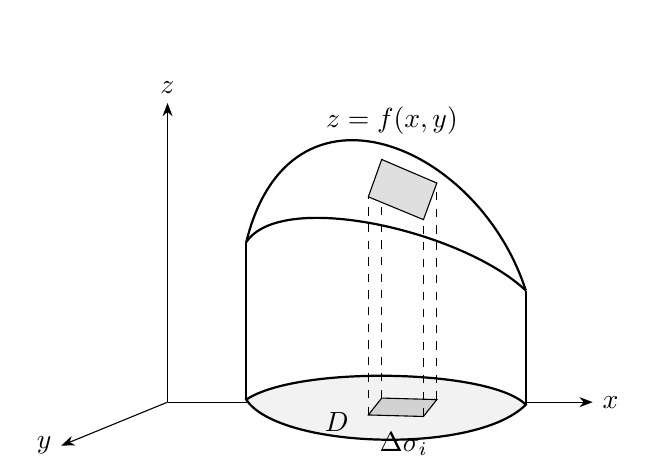
\begin{tikzpicture}[x=1cm,y=0.65cm,z={(0cm,1cm)},>=Stealth]
  \draw[->] (0,0,0) -- (5.4,0,0) node[right] {$x$};
  \draw[->] (0,0,0) -- (-1.35,-0.85,0) node[left] {$y$};
  \draw[->] (0,0,0) -- (0,0,3.8) node[above] {$z$};
  \fill[gray!10] (1.0,0.05,0) .. controls (1.4,-0.9,0) and (3.9,-1.05,0) .. (4.55,-0.05,0)
    .. controls (4.1,0.65,0) and (1.65,0.72,0) .. cycle;
  \draw[thick] (1.0,0.05,0) .. controls (1.4,-0.9,0) and (3.9,-1.05,0) .. (4.55,-0.05,0)
    .. controls (4.1,0.65,0) and (1.65,0.72,0) .. cycle;
  \draw[thick] (1.0,0.05,0) -- (1.0,0.05,2.0);
  \draw[thick] (4.55,-0.05,0) -- (4.55,-0.05,1.45);
  \draw[thick] (1.0,0.05,2.0) .. controls (1.45,-0.3,2.9) and (3.75,-0.5,2.5) .. (4.55,-0.05,1.45);
  \draw[thick] (1.0,0.05,2.0) .. controls (1.55,0.9,3.7) and (3.95,0.9,2.7) .. (4.55,-0.05,1.45);
  \node at (2.85,0.42,3.30) {$z=f(x,y)$};
  \node at (2.15,-0.38,0) {$D$};
  \fill[gray!35] (2.55,-0.25,0) -- (3.25,-0.28,0) -- (3.42,0.05,0) -- (2.72,0.08,0) -- cycle;
  \draw (2.55,-0.25,0) -- (3.25,-0.28,0) -- (3.42,0.05,0) -- (2.72,0.08,0) -- cycle;
  \draw[dashed] (2.55,-0.25,0) -- (2.55,-0.25,2.77);
  \draw[dashed] (3.25,-0.28,0) -- (3.25,-0.28,2.50);
  \draw[dashed] (3.42,0.05,0) -- (3.42,0.05,2.75);
  \draw[dashed] (2.72,0.08,0) -- (2.72,0.08,3.03);
  \fill[gray!25] (2.55,-0.25,2.77) -- (3.25,-0.28,2.50) -- (3.42,0.05,2.75) -- (2.72,0.08,3.03) -- cycle;
  \draw (2.55,-0.25,2.77) -- (3.25,-0.28,2.50) -- (3.42,0.05,2.75) -- (2.72,0.08,3.03) -- cycle;
  \node[below] at (3.0,-0.4,0) {$\Delta\sigma_i$};
\end{tikzpicture}
\end{center}

\begin{definition}[二重积分]
设函数 $f(x,y)$ 在有界闭区域 $D$ 上有定义。将 $D$ 分成 $n$ 个小区域 $\Delta D_i$，其面积记为 $\Delta\sigma_i$，各小区域的直径中的最大值记为 $\lambda$。在 $\Delta D_i$ 内任取一点 $(\xi_i,\eta_i)$。当 $\lambda\to0$ 时，若极限
\[
\lim_{\lambda\to0}\sum_{i=1}^n f(\xi_i,\eta_i)\Delta\sigma_i
\]
存在，且与区域的分法及点 $(\xi_i,\eta_i)$ 的取法无关，则称函数 $f(x,y)$ 在区域 $D$ 上\textbf{可积}。这个极限称为 $f(x,y)$ 在 $D$ 上的\textbf{二重积分}，记作
\[
\iint_D f(x,y)\,\dd\sigma
=\lim_{\lambda\to0}\sum_{i=1}^n f(\xi_i,\eta_i)\Delta\sigma_i.
\]
其中，$f(x,y)$ 称为\textbf{被积函数}，$D$ 称为\textbf{积分区域}，$\dd\sigma$ 称为\textbf{面积元素}。在直角坐标系中，通常写作
\[
\dd\sigma=\dd x\,\dd y,
\qquad
\iint_D f(x,y)\,\dd\sigma
=\iint_D f(x,y)\,\dd x\,\dd y.
\]
当 $f(x,y)\geq0$ 时，二重积分表示以 $D$ 为底、以 $z=f(x,y)$ 为顶的曲顶柱体体积。特别地，取 $f(x,y)=1$，有
\[
\iint_D\dd\sigma=\iint_D\dd x\,\dd y,
\]
其值就是区域 $D$ 的面积。
\end{definition}

如果 $f(x,y)$ 在有界闭区域 $D$ 上连续，则它在 $D$ 上可积。计算二重积分时，通常不直接按照定义作和式极限，而是把它化为两个定积分依次计算。为便于计算，先列出二重积分的常用性质。

\begin{theorem}[二重积分的性质]
设 $f(x,y)$ 与 $g(x,y)$ 在区域 $D$ 上可积，$k$ 为常数，则
\begin{enumerate}
\item 线性性：
\[
\iint_D\bigl[kf(x,y)+g(x,y)\bigr]\,\dd\sigma
=k\iint_Df(x,y)\,\dd\sigma+\iint_Dg(x,y)\,\dd\sigma;
\]
\item 可加性：若 $D$ 可分成除边界外没有公共部分的两个区域 $D_1,D_2$，则
\[
\iint_Df(x,y)\,\dd\sigma
=\iint_{D_1}f(x,y)\,\dd\sigma+\iint_{D_2}f(x,y)\,\dd\sigma;
\]
\item 保序性：若在 $D$ 上 $f(x,y)\leq g(x,y)$，则
\[
\iint_Df(x,y)\,\dd\sigma\leq\iint_Dg(x,y)\,\dd\sigma;
\]
\item 绝对值估计：
\[
\left|\iint_Df(x,y)\,\dd\sigma\right|
\leq\iint_D|f(x,y)|\,\dd\sigma;
\]
\item 积分中值性质：若 \(D\) 是面积为正的有界闭连通区域，且 \(f(x,y)\) 在 \(D\) 上连续，则存在点 \((\xi,\eta)\in D\)，使得
\[
\iint_Df(x,y)\,\dd\sigma=f(\xi,\eta)\iint_D\dd\sigma.
\]
\end{enumerate}
\end{theorem}

\begin{proof}
把各小区域上的和式分别写出即可得到线性性和可加性。保序性来自每一项
\[
f(\xi_i,\eta_i)\Delta\sigma_i
\leq g(\xi_i,\eta_i)\Delta\sigma_i,
\]
对所有小区域求和并取极限即得。由 $-|f|\leq f\leq|f|$ 以及保序性，有
\[
-\iint_D|f|\,\dd\sigma
\leq\iint_Df\,\dd\sigma
\leq\iint_D|f|\,\dd\sigma,
\]
从而得到绝对值估计。最后，设 \(D\) 是面积为正的有界闭连通区域。连续函数在 \(D\) 上能取得最大值 \(M\) 和最小值 \(m\)，于是
\[
m\leq\frac{1}{\iint_D\dd\sigma}\iint_Df(x,y)\,\dd\sigma\leq M.
\]
由于连通集在连续映射下的像仍为连通集，\(f(D)\) 是包含 \(m,M\) 的区间。因此存在 \((\xi,\eta)\in D\)，使上式中间的平均值等于 \(f(\xi,\eta)\)，即得积分中值性质。
\end{proof}

上述性质说明了二重积分可以进行拆分、比较和估计。实际计算时，还需要把它化为两个定积分依次计算，这就是累次积分。

\subsubsection*{累次积分}

\textbf{累次积分}是把二重积分化成两个定积分依次计算。关键是把积分区域用不等式准确表示出来。例如，若
\[
D=\{(x,y)\mid a\leq x\leq b,\ \varphi_1(x)\leq y\leq\varphi_2(x)\},
\]
则称 $D$ 为 $x$ 型区域。固定 $x$ 后，$y$ 从下边界 $\varphi_1(x)$ 变化到上边界 $\varphi_2(x)$，先对 $y$ 积分，再让 $x$ 在 $[a,b]$ 上变化，得到
\[
\iint_Df(x,y)\,\dd\sigma
=\int_a^b\left[\int_{\varphi_1(x)}^{\varphi_2(x)}f(x,y)\,\dd y\right]\dd x.
\]
也常简写为
\[
\iint_Df(x,y)\,\dd\sigma
=\int_a^b\dd x\int_{\varphi_1(x)}^{\varphi_2(x)}f(x,y)\,\dd y.
\]

如果区域可以表示为
\[
D=\{(x,y)\mid c\leq y\leq d,\ \psi_1(y)\leq x\leq\psi_2(y)\},
\]
则称 $D$ 为 $y$ 型区域，相应的计算公式为
\[
\iint_Df(x,y)\,\dd\sigma
=\int_c^d\left[\int_{\psi_1(y)}^{\psi_2(y)}f(x,y)\,\dd x\right]\dd y.
\]
在矩形区域 $D=[a,b]\times[c,d]$ 上，两种积分次序都可以使用：
\[
\iint_Df(x,y)\,\dd\sigma
=\int_a^b\dd x\int_c^df(x,y)\,\dd y
=\int_c^d\dd y\int_a^bf(x,y)\,\dd x.
\]

若积分区域不能直接表示为一个 $x$ 型区域或 $y$ 型区域，可以先把它分割成若干个标准区域，再利用二重积分的可加性分别计算。

计算累次积分可按以下顺序进行：先画出积分区域的草图，找出曲线交点；再分别尝试用竖直线段或水平线段穿过区域，确定积分次序和上下限；最后进行内层积分和外层积分。同一个二重积分有时可以按两种次序表示，应优先选择内层积分容易计算的一种。

\begin{example}[直角坐标下的累次积分]
计算
\[
I=\iint_D(x+y)\,\dd\sigma,
\]
其中 $D$ 是曲线 $y=x^2$ 与 $y=2x$ 所围成的区域。

两条曲线的交点满足 $x^2=2x$，所以 $x=0,2$。区域可表示为
\[
D=\{(x,y)\mid0\leq x\leq2,\ x^2\leq y\leq2x\}.
\]
因此
\[
\begin{aligned}
I&=\int_0^2\dd x\int_{x^2}^{2x}(x+y)\,\dd y\\
&=\int_0^2\left[xy+\frac{y^2}{2}\right]_{x^2}^{2x}\dd x\\
&=\int_0^2\left(4x^2-x^3-\frac12x^4\right)\dd x
=\frac{52}{15}.
\end{aligned}
\]

如果改用水平线段，则区域也可写成
\[
D=\left\{(x,y)\mid0\leq y\leq4,\ \frac y2\leq x\leq\sqrt y\right\}.
\]
于是
\[
I=\int_0^4\dd y\int_{y/2}^{\sqrt y}(x+y)\,\dd x,
\]
结果相同。由此可见，确定积分区域的表示方式是计算二重积分的基础，而积分次序的选择会直接影响计算过程的长短。
\end{example}

\begin{example}[根据被积函数选择积分次序]
计算
\[
I=\iint_D\frac{y}{(1+x^2+y^2)^{3/2}}\,\dd\sigma,
\qquad D=[0,1]\times[0,1].
\]

区域是矩形，两种次序都可以。观察被积函数，先对 $y$ 积分时容易出现 $1+x^2+y^2$ 的导数，因此取
\[
\begin{aligned}
I&=\int_0^1\dd x\int_0^1\frac{y}{(1+x^2+y^2)^{3/2}}\,\dd y\\
&=\frac12\int_0^1\left[\frac{-2}{\sqrt{1+x^2+y^2}}\right]_{y=0}^{y=1}\dd x\\
&=\int_0^1\left(\frac1{\sqrt{1+x^2}}-\frac1{\sqrt{2+x^2}}\right)\dd x\\
&=\ln(1+\sqrt2)-\ln\frac{1+\sqrt3}{\sqrt2}.
\end{aligned}
\]
若先对 $x$ 积分，内层积分会出现同样形式但计算较繁。所以，画出区域后还要结合被积函数观察积分次序。
\end{example}

在某些区域上，即使直接写出累次积分较为繁琐，也可以先观察区域和被积函数的对称性。若区域关于 $y$ 轴对称，而被积函数关于 $x$ 为奇函数，则二重积分为零；关于 $x$ 轴对称时有类似结论。

\begin{example}[利用对称性]
计算
\[
I=\iint_Dx(1+y^2)\,\dd\sigma,
\qquad D=\{(x,y)\mid -1\leq x\leq1,\ 0\leq y\leq1\}.
\]

区域 $D$ 关于 $y$ 轴对称，而被积函数关于 $x$ 为奇函数。因此
\[
I=0.
\]
\end{example}

直角坐标下的累次积分适合处理边界曲线容易表示为 $x$ 或 $y$ 的函数的区域。当区域边界含有圆、圆弧，或被积函数中出现 $x^2+y^2$ 时，可以改用极坐标描述积分区域和被积函数。

\subsubsection*{在极坐标系下计算二重积分}

当积分区域的边界含有圆或圆弧，或者被积函数中出现 $x^2+y^2$ 时，使用极坐标往往能同时简化积分区域和被积函数。平面上一点 $P$ 的极坐标记为 $(r,\theta)$，其中 $r$ 是 $P$ 到原点的距离，$\theta$ 是射线 $OP$ 从 $x$ 轴正向转过的角度。通常取
\[
r\geq0,\qquad 0\leq\theta<2\pi.
\]
极坐标与直角坐标之间的关系为
\[
x=r\cos\theta,\qquad y=r\sin\theta,
\]
从而
\[
r=\sqrt{x^2+y^2},\qquad x^2+y^2=r^2.
\]
同一个点的极角可以相差 $2\pi$ 的整数倍；原点的极角没有唯一取值。因此，在表示积分区域时，应选择一段合适的角度区间，使除边界上的少数点外，区域中的点只被表示一次。

\begin{custom}{曲线与区域的极坐标表示}
把曲线的直角坐标方程中的 $x,y$ 分别换成 $r\cos\theta,r\sin\theta$，即可得到相应的极坐标方程。例如，
\[
x^2+y^2=a^2
\]
化为 $r=a$；当 $a>0$ 时，
\[
x^2+y^2=2ax
\]
化为
\[
r=2a\cos\theta.
\]
对于平面区域，也应先画出草图，再沿着从原点出发的射线观察该射线进入和离开区域时的半径。
\end{custom}

\begin{example}[区域的极坐标表示]
将区域
\[
D=\{(x,y)\mid 1\leq x^2+y^2\leq2x,\ y\geq0\}
\]
用极坐标表示。

两个边界圆分别化为
\[
r=1,\qquad r=2\cos\theta.
\]
由于 $y\geq0$，只考虑上半平面；同时必须满足
\[
1\leq2\cos\theta.
\]
结合区域草图可知
\[
0\leq\theta\leq\frac{\pi}{3},\qquad
1\leq r\leq2\cos\theta.
\]
因此，区域 $D$ 的极坐标表示为
\[
\Omega=\left\{(r,\theta)\,\middle|\,
0\leq\theta\leq\frac{\pi}{3},\
1\leq r\leq2\cos\theta\right\}.
\]
\end{example}

\begin{custom}{极坐标下的面积元素}
在极坐标网格中，用半径分别为 $r$ 和 $r+\Delta r$ 的两个圆以及极角分别为 $\theta$ 和 $\theta+\Delta\theta$ 的两条射线围成一个小曲边四边形。它的面积等于两个扇形面积之差，即
\[
\Delta\sigma
=\frac12\bigl[(r+\Delta r)^2-r^2\bigr]\Delta\theta
=r\,\Delta r\,\Delta\theta
+ \frac12(\Delta r)^2\Delta\theta.
\]
当 $\Delta r$ 和 $\Delta\theta$ 都很小时，后一项相对于前一项可以忽略，因而
\[
\Delta\sigma\approx r\,\Delta r\,\Delta\theta.
\]
在分割不断加细的极限过程中，极坐标下的面积元素为
\[
\boxed{\dd\sigma=r\,\dd r\,\dd\theta}.
\]
因子 $r$ 反映了同样的角度增量在离原点较远处会扫过更长的圆弧，计算时不能遗漏。
\end{custom}

于是，若区域 $D$ 在极坐标下表示为 $\Omega$，则
\[
\boxed{\iint_D f(x,y)\,\dd\sigma
=\iint_\Omega
f(r\cos\theta,r\sin\theta)\,r\,\dd r\,\dd\theta}.
\]
这个公式可以直接由二重积分的分割求和理解，不需要借助矩阵或行列式。

\begin{custom}{极坐标区域的三种常见类型}
\begin{enumerate}
\item 若原点在区域内部，并且边界可写成 $r=\rho(\theta)$，则常取
\[
0\leq\theta\leq2\pi,\qquad 0\leq r\leq\rho(\theta).
\]
\item 若区域位于两条曲线 $r=r_1(\theta)$ 与 $r=r_2(\theta)$ 之间，则常取
\[
\alpha\leq\theta\leq\beta,\qquad
r_1(\theta)\leq r\leq r_2(\theta).
\]
\item 若原点在区域边界上，并且区域由两条射线与曲线 $r=\rho(\theta)$ 围成，则常取
\[
\alpha\leq\theta\leq\beta,\qquad 0\leq r\leq\rho(\theta).
\]
\end{enumerate}
这些形式都以 $\theta$ 为外层变量、$r$ 为内层变量。若一个区域不能用一组连续的半径范围表示，应先把它分成若干部分。
\end{custom}

使用极坐标计算二重积分时，可以按以下步骤进行：先画出区域草图；把边界方程改写成极坐标形式；确定射线扫过的角度范围以及每条射线上的内外半径；把被积函数中的 $x,y$ 换成 $r\cos\theta,r\sin\theta$；最后写出面积元素中的因子 $r$。

\begin{example}[圆环区域上的二重积分]
计算
\[
I=\iint_D \ee^{-(x^2+y^2)}\,\dd\sigma,
\qquad D=\{(x,y)\mid1\leq x^2+y^2\leq4\}.
\]

区域 $D$ 是以原点为圆心、内半径为 $1$、外半径为 $2$ 的圆环。在极坐标下，
\[
1\leq r\leq2,\qquad0\leq\theta\leq2\pi.
\]
因此
\[
\begin{aligned}
I&=\int_0^{2\pi}\dd\theta\int_1^2\ee^{-r^2}r\,\dd r\\
&=2\pi\left[-\frac12\ee^{-r^2}\right]_1^2
=\pi(\ee^{-1}-\ee^{-4}).
\end{aligned}
\]
极坐标同时简化了积分区域和被积函数。
\end{example}

\begin{example}[偏心圆区域上的二重积分]
计算
\[
I=\iint_Dxy\,\dd\sigma,
\]
其中 $D$ 是圆域 $x^2+y^2\leq2x$ 位于 $x$ 轴上方的部分。

将圆的方程化为极坐标形式：
\[
r^2=2r\cos\theta,\qquad r=2\cos\theta.
\]
由于只取 $x$ 轴上方的半圆，有
\[
0\leq\theta\leq\frac\pi2,\qquad0\leq r\leq2\cos\theta.
\]
又 $xy=r^2\cos\theta\sin\theta$，所以
\[
\begin{aligned}
I&=\int_0^{\pi/2}\dd\theta\int_0^{2\cos\theta}
r^3\cos\theta\sin\theta\,\dd r\\
&=4\int_0^{\pi/2}\cos^5\theta\sin\theta\,\dd\theta
=\frac23.
\end{aligned}
\]
对于圆心不在原点的圆域，仍可先把边界方程化为极坐标形式。若极坐标边界较简单，则应先由边界方程确定 $r$ 的范围，再确定 $\theta$ 的范围。
\end{example}

\subsubsection*{面积密度型应用}

二重积分不仅表示曲顶柱体体积，还可以累积二维区域上的密度。若 $q(x,y)$ 表示单位面积上的某种量，则区域 $D$ 内的总量为
\[
Q=\iint_D q(x,y)\,\dd A.
\]

\begin{application}[工程：薄板总质量]
设矩形薄板 $D=[0,1]\times[0,2]$ 的面密度为
\[
\rho(x,y)=1+x+y\quad(\mathrm{kg/m^2}),
\]
其中 $x,y$ 的单位为 $\mathrm m$。忽略厚度变化，则
\[
\begin{aligned}
M&=\iint_D\rho(x,y)\,\dd A\\
&=\int_0^1\int_0^2(1+x+y)\,\dd y\,\dd x
=5\ \mathrm{kg}.
\end{aligned}
\]
积分中的“面密度乘小面积”具有质量单位，所有小块累加便得到总质量。
\end{application}

\begin{application}[农业与医学：区域总量]
若 $f(x,y)$ 是田块上的施肥面密度，单位为 $\mathrm{kg/m^2}$，则总施肥量为
\[
F=\iint_D f(x,y)\,\dd A,
\qquad [F]=\mathrm{kg}.
\]
模型假设面密度可由可积函数近似；真实施用还会受到设备轨迹、风和地形影响。类似地，若二维截面上的剂量密度或信号强度为 $I(x,y)$，则区域总量可写为
\[
Q=\iint_D I(x,y)\,\dd A.
\]
后一公式只说明面积密度的数学累积方式，不涉及具体临床治疗剂量设计。
\end{application}

\subsubsection*{反常二重积分}

本书只讨论最常见且理论较稳定的情形：$f(x,y)\geq0$，或已经知道
\[
\iint_D|f(x,y)|\,\dd\sigma<+\infty.
\]
在这些情况下，可以通过一列不断扩大的有界区域理解反常二重积分。对于一般符号变化的函数，若不能保证绝对可积，积分值可能依赖于区域的扩张方式，本书不展开讨论。

设 $D_R$ 是一列有界区域，满足
\[
D_R\subset D_{R'}\subset D\quad(R<R'),
\qquad
\bigcup_{R>0}D_R=D.
\]
若 $f\geq0$，定义
\[
\iint_Df(x,y)\,\dd\sigma
=\lim_{R\to+\infty}\iint_{D_R}f(x,y)\,\dd\sigma,
\]
其中极限允许为 $+\infty$；若该极限有限，则称反常二重积分收敛。若 $f$ 已知绝对可积，也可用同样的有界区域逼近理解其积分。

\begin{example}[全平面上的反常二重积分]
计算
\[
I=\iint_{\RR^2}\ee^{-(x^2+y^2)}\,\dd\sigma.
\]

取 $D_R$ 为以原点为圆心、半径为 $R$ 的圆域。在极坐标下，
\[
\begin{aligned}
I&=\lim_{R\to+\infty}\int_0^{2\pi}\dd\theta\int_0^R \ee^{-r^2}r\,\dd r\\
&=\lim_{R\to+\infty}2\pi\left[-\frac12\ee^{-r^2}\right]_0^R
=\pi.
\end{aligned}
\]
\end{example}

\subsubsection*{跨学科拓展：极坐标换元在概率统计中的应用}

\begin{extra}
本节为选读内容，需要读者了解概率密度、联合分布与随机变量独立性的基本概念。

极坐标不仅适合处理圆形积分区域，还能揭示二维正态分布的径向结构。下面先用反常二重积分计算高斯积分，再讨论二维正态随机变量的半径分布以及生成正态随机数的 Box--Muller 变换。

\begin{example}[高斯积分与正态分布的归一化常数]
对 $R>0$，记
\[
G_R=\int_{-R}^{R}\ee^{-x^2/2}\,\dd x,
\qquad
G=\lim_{R\to+\infty}G_R.
\]
设 $Q_R=[-R,R]\times[-R,R]$，并以 $D_R$ 表示以原点为圆心、半径为 $R$ 的圆域。把两个有限区间上的积分相乘，得到
\[
G_R^2
=\iint_{Q_R}\ee^{-(x^2+y^2)/2}\,\dd\sigma.
\]
由于
\[
D_R\subset Q_R\subset D_{\sqrt2R},
\]
并且被积函数非负，所以
\[
\iint_{D_R}\ee^{-(x^2+y^2)/2}\,\dd\sigma
\leq G_R^2\leq
\iint_{D_{\sqrt2R}}\ee^{-(x^2+y^2)/2}\,\dd\sigma.
\]
在圆域上使用极坐标可得
\[
\begin{aligned}
\iint_{D_R}\ee^{-(x^2+y^2)/2}\,\dd\sigma
&=\int_0^{2\pi}\dd\theta\int_0^R\ee^{-r^2/2}r\,\dd r\\
&=2\pi\bigl(1-\ee^{-R^2/2}\bigr).
\end{aligned}
\]
把上式中的 $R$ 换成 $\sqrt2R$，夹逼不等式的左右两端在 $R\to+\infty$ 时都趋于 $2\pi$。因此 $G_R^2\to2\pi$。又因为 $G_R>0$，所以
\[
\boxed{G=\sqrt{2\pi}}.
\]
再令 $x=\sigma t$，其中 $\sigma>0$，可得
\[
\int_{-\infty}^{+\infty}
\ee^{-x^2/(2\sigma^2)}\,\dd x
=\sigma\sqrt{2\pi}.
\]
所以
\[
f_X(x)=\frac{1}{\sqrt{2\pi}\sigma}
\ee^{-x^2/(2\sigma^2)},\qquad -\infty<x<+\infty,
\]
在全实数轴上的积分等于 $1$，这就是均值为 $0$、方差为 $\sigma^2$ 的正态分布密度中的归一化常数。
\end{example}

\begin{example}[二维正态分布、独立性与瑞利分布]
设 $X,Y$ 相互独立，并且
\[
X,Y\sim\mathcal N(0,\sigma^2),\qquad \sigma>0.
\]
由独立性，二者的联合概率密度等于各自密度的乘积：
\[
\begin{aligned}
f_{X,Y}(x,y)
&=f_X(x)f_Y(y)\\
&=\frac{1}{2\pi\sigma^2}
\exp\left(-\frac{x^2+y^2}{2\sigma^2}\right).
\end{aligned}
\]
令
\[
R=\sqrt{X^2+Y^2},\qquad
\Theta=\text{点 $(X,Y)$ 的极角},
\]
其中 $R\geq0,\ 0\leq\Theta<2\pi$。极坐标中的小区域面积为 $r\,\dd r\,\dd\theta$，因此 $(R,\Theta)$ 的联合密度为
\[
\begin{aligned}
f_{R,\Theta}(r,\theta)
&=f_{X,Y}(r\cos\theta,r\sin\theta)\,r\\
&=\frac{r}{2\pi\sigma^2}
\exp\left(-\frac{r^2}{2\sigma^2}\right),
\end{aligned}
\]
其中 $r\geq0,\ 0\leq\theta<2\pi$；在其他位置密度为 $0$。上式可以分解为
\[
f_{R,\Theta}(r,\theta)
=\underbrace{\frac{r}{\sigma^2}
\exp\left(-\frac{r^2}{2\sigma^2}\right)}_{f_R(r)}
\underbrace{\frac{1}{2\pi}}_{f_\Theta(\theta)}.
\]
因此 $R$ 与 $\Theta$ 相互独立，$\Theta$ 在 $[0,2\pi)$ 上服从均匀分布，而 $R$ 的密度为
\[
\boxed{f_R(r)=\frac{r}{\sigma^2}
\exp\left(-\frac{r^2}{2\sigma^2}\right),\qquad r\geq0}.
\]
这称为参数为 $\sigma$ 的\textbf{瑞利分布}。其分布函数为
\[
F_R(r)
=\int_0^r\frac{s}{\sigma^2}
\ee^{-s^2/(2\sigma^2)}\,\dd s
=1-\ee^{-r^2/(2\sigma^2)},\qquad r\geq0.
\]
例如，把 $X,Y$ 看作二维平面上相互垂直方向的射击误差时，$R$ 表示落点到靶心的距离；把它们看作复高斯白噪声的实部和虚部时，$R$ 表示复数噪声的幅值。
\end{example}

\begin{custom}{Box--Muller 变换}
设 $U_1,U_2$ 是相互独立的 $(0,1)$ 上均匀分布随机变量。定义
\[
R=\sigma\sqrt{-2\ln U_1},\qquad
\Theta=2\pi U_2,
\]
再令
\[
\boxed{
\begin{aligned}
Z_1&=R\cos\Theta
=\sigma\sqrt{-2\ln U_1}\cos(2\pi U_2),\\
Z_2&=R\sin\Theta
=\sigma\sqrt{-2\ln U_1}\sin(2\pi U_2).
\end{aligned}}
\]
因为
\[
\begin{aligned}
\Pr\{R\leq r\}
&=\Pr\left\{\sigma\sqrt{-2\ln U_1}\leq r\right\}\\
&=\Pr\left\{U_1\geq
\ee^{-r^2/(2\sigma^2)}\right\}\\
&=1-\ee^{-r^2/(2\sigma^2)},\qquad r\geq0,
\end{aligned}
\]
所以 $R$ 服从参数为 $\sigma$ 的瑞利分布；同时 $\Theta$ 在 $[0,2\pi)$ 上均匀分布，并且 $R$ 与 $\Theta$ 相互独立。再利用极坐标小区域的面积关系
\[
\dd z_1\,\dd z_2=r\,\dd r\,\dd\theta,
\]
可得 \((Z_1,Z_2)\) 的联合密度
\[
f_{Z_1,Z_2}(z_1,z_2)
=\frac{1}{2\pi\sigma^2}
\exp\left(-\frac{z_1^2+z_2^2}{2\sigma^2}\right)
=f_{Z_1}(z_1)f_{Z_2}(z_2).
\]
因此 $Z_1,Z_2$ 相互独立，且都服从 $\mathcal N(0,\sigma^2)$。取 $\sigma=1$ 就能由两个独立均匀随机数生成两个独立的标准正态随机数，这就是 Box--Muller 变换。
\end{custom}

\end{extra}

\begin{custom}{二重积分的计算思路}
计算二重积分可按以下顺序观察：
\begin{enumerate}
\item 画出积分区域 $D$ 的草图，标出边界曲线和交点；若区域不是标准区域，先分割成若干个标准区域；
\item 根据区域形状、被积函数特点和对称性，选择直角坐标或极坐标；
\item 若使用直角坐标，确定采用竖直切片还是水平切片，并写出累次积分；
\item 若使用极坐标，确定 $r$ 和 $\theta$ 的范围，同时写出面积元素 $r\,\dd r\,\dd\theta$；
\item 先计算容易处理的内层积分，再计算外层积分。
\end{enumerate}
二重积分题的关键通常在积分区域的表示。积分式确定以后，其后的运算就转化为已经熟悉的一元积分。
\end{custom}

\iffalse


\clearpage
\subsection*{第8章课后习题}
\addcontentsline{toc}{subsection}{第8章课后习题}

\subsubsection*{第8.1--8.6节\quad 定积分与反常积分}

\begin{enumerate}
\item[]\textbf{A.\ 定积分的性质与黎曼和}
\item 不计算积分，比较下列各组定积分的大小：
\begin{enumerate}
\item[(1)] $\displaystyle \int_0^1x^3\,\dd x$ 与 $\displaystyle \int_0^1x^6\,\dd x$；
\item[(2)] $\displaystyle \int_1^2x^2\,\dd x$ 与 $\displaystyle \int_1^2x^4\,\dd x$；
\item[(3)] $\displaystyle \int_0^{\pi/2}x\,\dd x$ 与 $\displaystyle \int_0^{\pi/2}\sin x\,\dd x$；
\item[(4)] $\displaystyle \int_0^1\ee^x\,\dd x$ 与 $\displaystyle \int_0^1\ee^{x^2}\,\dd x$；
\item[(5)] $\displaystyle \int_0^1\ee^{-x}\,\dd x$ 与 $\displaystyle \int_0^1\ee^{-x^2}\,\dd x$；
\item[(6)] $\displaystyle \int_0^{\pi/2}\sin^2x\,\dd x$ 与 $\displaystyle \int_0^{\pi/2}\sin^4x\,\dd x$。
\end{enumerate}

\item 利用定积分的性质，估计下列积分的范围：
\begin{enumerate}
\item[(1)] $\displaystyle \int_{-a}^{a}\ee^{-x^2}\,\dd x\quad(a>0)$；
\item[(2)] $\displaystyle \int_{\pi/6}^{\pi/3}(1+\cos^2x)\,\dd x$；
\item[(3)] $\displaystyle \int_1^2\frac{\ln x}{x}\,\dd x$；
\item[(4)] $\displaystyle \int_0^1\frac{x^5}{\sqrt{1+x}}\,\dd x$；
\item[(5)] $\displaystyle \int_0^{100}\frac{1}{x+10\ee^{-x}}\,\dd x$。
\end{enumerate}

\item 用定积分定义或定积分性质求下列极限：
\begin{enumerate}
\item[(1)] $\displaystyle \lim_{n\to\infty}\frac1n\sum_{k=1}^{n}\sin\frac{k}{n}$；
\item[(2)] $\displaystyle \lim_{n\to\infty}\frac1n\sum_{k=0}^{n-1}\ee^{2k/n}$；
\item[(3)] $\displaystyle \lim_{n\to\infty}\left(\frac1{n+1}+\frac1{n+2}+\cdots+\frac1{2n}\right)$；
\item[(4)] $\displaystyle \lim_{x\to0}\frac1x\int_0^x(1+\sin 2u)^{1/u}\,\dd u$；
\item[(5)] $\displaystyle \lim_{x\to0}\frac1{x^2}\int_0^x\arctan u\,\dd u$。
\end{enumerate}

\item[]\textbf{B.\ 微积分基本定理与积分上限函数}
\setcounter{enumi}{0}
\par\smallskip
\noindent\textbf{含参积分与积分号下求导（选做）}\quad
在相应函数连续且偏导连续的条件下，固定积分限时有
\[
\frac{\dd}{\dd x}\int_a^b f(x,t)\,\dd t
=\int_a^b\frac{\partial f}{\partial x}(x,t)\,\dd t.
\]
若积分限也依赖于 $x$，则
\[
\frac{\dd}{\dd x}\int_{\alpha(x)}^{\beta(x)}f(x,t)\,\dd t
=f\bigl(x,\beta(x)\bigr)\beta'(x)
-f\bigl(x,\alpha(x)\bigr)\alpha'(x)
+\int_{\alpha(x)}^{\beta(x)}\frac{\partial f}{\partial x}(x,t)\,\dd t.
\]
上述公式只作为拓展，不纳入本章基本要求。
\item 求下列函数的导数：
\begin{enumerate}
\item[(1)] $\displaystyle y=\int_0^{x^2}\sqrt{1+t^4}\,\dd t$；
\item[(2)] $\displaystyle y=\int_x^{\sin x}\frac{\dd t}{\sqrt{1+t^2}}$；
\item[(3)] $\displaystyle y=\int_{\cos x}^{x^2}\ee^{-t^2}\,\dd t$；
\item[(4)] $\displaystyle y=\int_1^2\ln(1+xt)\,\dd t\quad\left(x>-\frac12,\ \text{选做}\right)$；
\item[(5)] $\displaystyle y=\int_{x}^{x+1}\frac{\sin(xt)}{1+t^2}\,\dd t\quad\text{（选做）}$。
\end{enumerate}

\item 利用牛顿--莱布尼茨公式计算下列定积分：
\begin{enumerate}
\item[(1)] $\displaystyle \int_0^2(3x^2-2x+1)\,\dd x$；
\item[(2)] $\displaystyle \int_1^2\frac{1+x^3}{x^2+x^3}\,\dd x$；
\item[(3)] $\displaystyle \int_0^2(\ee^x-x)\,\dd x$；
\item[(4)] $\displaystyle \int_0^1|2x-1|\,\dd x$；
\item[(5)] $\displaystyle \int_a^b|x|\,\dd x\quad(a<0<b)$；
\item[(6)] $\displaystyle \int_a^b|2x-a-b|\,\dd x\quad(a<b)$；
\item[(7)] $\displaystyle \int_0^\pi \sin^2x\,\dd x$；
\item[(8)] $\displaystyle \int_{-\pi/2}^{\pi/2}(x^3+\cos x)\,\dd x$。
\end{enumerate}

\item[]\textbf{C.\ 定积分的换元法}
\setcounter{enumi}{0}
\item 用换元法计算下列定积分：
\begin{enumerate}
\item[(1)] $\displaystyle \int_0^{\pi/2}\cos\frac{x}{2}\cos\frac{3x}{2}\,\dd x$；
\item[(2)] $\displaystyle \int_0^{\ln2}\sqrt{\ee^x-1}\,\dd x$；
\item[(3)] $\displaystyle \int_1^{\sqrt5}\frac{\sqrt{x^2-1}}{x}\,\dd x$；
\item[(4)] $\displaystyle \int_1^\ee\frac{\dd x}{x\sqrt{1+\ln x}}$；
\item[(5)] $\displaystyle \int_0^1\frac{\dd x}{1+x^2}$；
\item[(6)] $\displaystyle \int_0^2\frac{x\,\dd x}{\sqrt{1+x^2}}$；
\item[(7)] $\displaystyle \int_0^1\frac{x\,\dd x}{1+x^4}$；
\item[(8)] $\displaystyle \int_0^1\frac{x^3}{\sqrt{1-x^2}}\,\dd x$；
\item[(9)] $\displaystyle \int_1^4\frac{\sqrt{x}}{1+\sqrt{x}}\,\dd x$；
\item[(10)] $\displaystyle \int_0^{\pi/4}\tan x\,\dd x$；
\item[(11)] $\displaystyle \int_0^1x\sqrt{1-x^2}\,\dd x$；
\item[(12)] $\displaystyle \int_0^{1/2}\frac{\dd x}{\sqrt{1-x^2}}$。
\end{enumerate}

\item[]\textbf{D.\ 定积分的分部积分法}
\setcounter{enumi}{0}
\item 用分部积分法计算下列定积分：
\begin{enumerate}
\item[(1)] $\displaystyle \int_0^1(x-1)^3x\,\dd x$；
\item[(2)] $\displaystyle \int_0^{\pi/2}x\sin x\,\dd x$；
\item[(3)] $\displaystyle \int_1^\ee\ln x\,\dd x$；
\item[(4)] $\displaystyle \int_0^1\ln(1+x)\,\dd x$；
\item[(5)] $\displaystyle \int_0^1x\ee^{-2x}\,\dd x$；
\item[(6)] $\displaystyle \int_1^\ee x(\ln x)^2\,\dd x$；
\item[(7)] $\displaystyle \int_0^{\pi/2}x\cos x\,\dd x$；
\item[(8)] $\displaystyle \int_0^\pi \ee^x\sin x\,\dd x$。
\end{enumerate}

\item[]\textbf{E.\ 对称性与综合计算}
\setcounter{enumi}{0}
\item 利用对称性、周期性或换元技巧计算下列积分：
\begin{enumerate}
\item[(1)] $\displaystyle \int_0^{\pi/2}\frac{\sin x}{\sin x+\cos x}\,\dd x$；
\item[(2)] $\displaystyle \int_0^\pi\frac{x\sin x}{1+\cos^2x}\,\dd x$；
\item[(3)] $\displaystyle \int_{-\pi}^{\pi}\frac{x^3+\sin x}{1+x^2}\,\dd x$；
\item[(4)] $\displaystyle \int_0^{3\pi}|\sin x|\,\dd x$。
\end{enumerate}

\item 计算下列定积分：
\begin{enumerate}
\item[(1)] $\displaystyle \int_{-2}^{2}|x^2-1|\,\dd x$；
\item[(2)] $\displaystyle \int_{\ee^{-1}}^{\ee}|\ln x|\,\dd x$；
\item[(3)] $\displaystyle \int_1^{16}\arctan\sqrt{x-1}\,\dd x$；
\item[(4)] $\displaystyle \int_0^1\ln(1+\sqrt{x})\,\dd x$；
\item[(5)] $\displaystyle \int_0^{\pi}\sin^2x\cos nx\,\dd x\quad(n\in\mathbb N^+)$；
\item[(6)] $\displaystyle \int_0^1\frac{\ln(1+x)}{1+x^2}\,\dd x$。
\end{enumerate}

\item 证明下列结论：
\begin{enumerate}
\item[(1)] 若 $f(x)$ 在 $[a,b]$ 上连续且不恒为 $0$，并且 $f(x)\geq0$，证明 $\displaystyle \int_a^b f(x)\,\dd x>0$；
\item[(2)] 设 $f(x)$ 连续，证明 $\displaystyle \int_a^b f(x)\,\dd x=(b-a)\int_0^1f(a+(b-a)t)\,\dd t$；
\item[(3)] 设 $f(x)$ 连续，证明 $\displaystyle \int_0^a x^3f(x^2)\,\dd x=\frac12\int_0^{a^2}uf(u)\,\dd u\quad(a>0)$；
\item[(4)] 若 $f(x)$ 为偶函数，证明 $\displaystyle \int_0^x f(t)\,\dd t$ 为奇函数；若 $f(x)$ 为奇函数，证明 $\displaystyle \int_0^x f(t)\,\dd t$ 为偶函数。
\end{enumerate}

\item[]\textbf{F.\ 几何与实际应用}
\setcounter{enumi}{0}
\item 求下列平面图形的面积：
\begin{enumerate}
\item[(1)] $y=x$ 与 $y=x^2$ 围成的图形；
\item[(2)] $y=2x^2+3x-5$ 与 $y=1-x^2$ 围成的图形；
\item[(3)] $y=3x^2-1$ 与 $y=5-3x$ 围成的图形；
\item[(4)] $xy=6$ 与 $x+y=7$ 在第一象限围成的图形；
\item[(5)] \(y=\ln x,\ y=0,\ x=\ee\) 围成的图形；
\item[(6)] $x=y^2$ 与 $x=2-y$ 围成的图形。
\end{enumerate}

\item 求下列立体的体积：
\begin{enumerate}
\item[(1)] 某立体垂直于 $x$ 轴的截面都是正方形，截面边长为 $\sqrt{1+x}$，$0\leq x\leq3$；
\item[(2)] 某立体垂直于 $x$ 轴的截面都是圆，截面半径为 $r(x)=1+x$，$0\leq x\leq1$；
\item[(3)] 由 $y=x^2,\ x=0,\ x=1$ 与 $x$ 轴围成的曲边梯形绕 $x$ 轴旋转一周所得旋转体；
\item[(4)] 由 $y=x^2,\ y=1$ 与 $y$ 轴围成的图形绕 $y$ 轴旋转一周所得旋转体；
\item[(5)] 由 $y=\sin x,\ y=0,\ 0\leq x\leq\pi$ 围成的图形绕 $x$ 轴旋转一周所得旋转体；
\item[(6)] 由 $y=x,\ y=x^2$ 围成的图形绕 $x$ 轴旋转一周所得旋转体。
\end{enumerate}

\item 解下列应用题：
\begin{enumerate}
\item[(1)] 某产品上市后第 $t$ 年的年销售率为 $f(t)=1200-300\ee^{-t}$，求前 $5$ 年的总销售量；
\item[(2)] 某产品的边际收益为 $R'(Q)=8(12-Q)\ee^{-Q/10}$，求销售量从 $0$ 增加到 $6$ 时收益的增加量；
\item[(3)] 某产品的边际成本和边际收益分别为 $C'(Q)=Q^2-4Q+6,\ R'(Q)=100-2Q$，固定成本为 $80$，求利润函数，并求最大利润对应的销售量；
\item[(4)] 一物体沿直线运动，速度为 $v(t)=t^2-2t+2$，求 $0\leq t\leq3$ 内经过的路程；
\item[(5)] 某物体从 $x=0$ 移动到 $x=4$，所受变力为 $F(x)=3x^2+1$，方向与运动方向一致，求该力所做的功。
\end{enumerate}

\item[]\textbf{G.\ 反常积分}
\setcounter{enumi}{0}
\item 判断下列反常积分的敛散性；若收敛，求其值：
\begin{enumerate}
\item[(1)] $\displaystyle \int_0^{+\infty}\ee^{-2x}\,\dd x$；
\item[(2)] $\displaystyle \int_1^{+\infty}\frac{\dd x}{x(\ln x)^2}$；
\item[(3)] $\displaystyle \int_0^1\ln x\,\dd x$；
\item[(4)] $\displaystyle \int_0^1\frac{\dd x}{\sqrt{x}}$；
\item[(5)] $\displaystyle \int_1^2\frac{\dd x}{x^2-3x+2}$；
\item[(6)] $\displaystyle \int_0^{+\infty}\cos x\,\dd x$；
\item[(7)] $\displaystyle \int_0^1\frac{\dd x}{x^p}\quad(p>0)$；
\item[(8)] $\displaystyle \int_1^{+\infty}\frac{\dd x}{x^p}\quad(p>0)$。
\end{enumerate}

\item[]\textbf{H.\ 提高题与选做题}
\setcounter{enumi}{0}
\item 计算下列与 $\Gamma$ 函数和 $\mathrm B$ 函数有关的积分：
\begin{enumerate}
\item[(1)] $\displaystyle \Gamma(5)$；
\item[(2)] $\displaystyle \int_0^{+\infty}x^2\ee^{-x}\,\dd x$；
\item[(3)] $\displaystyle \int_0^{+\infty}x^3\ee^{-2x}\,\dd x$；
\item[(4)] $\displaystyle \mathrm B(2,4)$；
\item[(5)] $\displaystyle \int_0^1x^{1/2}(1-x)^2\,\dd x$。
\end{enumerate}

\item 设 $f(x)$ 连续，完成下列证明或计算：
\begin{enumerate}
\item[(1)] 证明 $\displaystyle \int_0^1\left(\int_0^t f(u)\,\dd u\right)\dd t=\int_0^1(1-u)f(u)\,\dd u$；
\item[(2)] 设 $x>0$，且 $f(t)>0$。若 $\displaystyle F(x)=\frac{\int_0^x tf(t)\,\dd t}{\int_0^x f(t)\,\dd t}$，说明 $F(x)$ 可看成区间 $[0,x]$ 上关于权重 $f(t)$ 的平均位置，并证明 $0<F(x)<x$；
\item[(3)] 设 $\displaystyle S(x)=\int_0^x|\cos t|\,\dd t$，求 $\displaystyle \lim_{x\to+\infty}\frac{S(x)}x$。
\end{enumerate}
\end{enumerate}

\subsubsection*{第8.7节\quad 二重积分}


\begin{enumerate}
\item[]\textbf{A.\ 积分区域与累次积分}
\item 写出下列区域的两种累次积分表示：
\begin{enumerate}
\item[(1)] $D$ 是由曲线 $y=x^2$ 与 $y=2x$ 所围成的区域；
\item[(2)] $D$ 是第一象限内由直线 $x=0,y=1$ 与曲线 $y=x^2$ 所围成的区域。
\end{enumerate}

\item 改变下列累次积分的积分次序：
\begin{enumerate}
\item[(1)]
\[
\int_0^1\dd x\int_x^{\sqrt{x}}f(x,y)\,\dd y;
\]
\item[(2)]
\[
\int_0^1\dd y\int_{y^2}^{y}f(x,y)\,\dd x.
\]
\end{enumerate}

\item[]\textbf{B.\ 直角坐标计算}
\setcounter{enumi}{0}
\item 计算下列直角坐标下的二重积分：
\begin{enumerate}
\item[(1)]
\[
\int_0^1\dd x\int_0^2(x^2+y^2)\,\dd y;
\]
\item[(2)]
\[
\int_1^2\dd x\int_x^{\sqrt{3x}}xy\,\dd y;
\]
\item[(3)]
\[
\int_0^1\dd x\int_0^{2-x}(x+2y)\,\dd y;
\]
\item[(4)]
\[
\int_0^2\dd y\int_0^{y/2}x^2y\,\dd x;
\]
\item[(5)]
\[
\iint_Dxy\,\dd\sigma,
\]
其中 $D$ 是由 $y=x$，$y=3x$ 和 $x=1$ 围成的区域；
\item[(6)]
\[
\iint_D\frac{x}{(1+x^2+y^2)^2}\,\dd\sigma,
\]
其中 $D=[0,1]\times[0,2]$；
\item[(7)]
\[
\iint_D\frac{y}{\sqrt{1+x^2+y^2}}\,\dd\sigma,
\]
其中 $D$ 是由 $x=0,y=0,x=1,y=1$ 围成的正方形区域。
\end{enumerate}

\item[]\textbf{C.\ 对称性}
\setcounter{enumi}{0}
\item 利用对称性计算下列二重积分：
\begin{enumerate}
\item[(1)]
\[
\iint_Dy\,\dd\sigma,
\qquad D=\{(x,y)\mid x^2+y^2\leq1\};
\]
\item[(2)]
\[
\iint_Dx(1+y^2)\,\dd\sigma,
\qquad D=\{(x,y)\mid-1\leq x\leq1,\ 0\leq y\leq1\};
\]
\item[(3)]
\[
\iint_D(x^2-y^2)\,\dd\sigma,
\qquad D=\{(x,y)\mid x^2+y^2\leq1\}.
\]
\end{enumerate}

\item[]\textbf{D.\ 极坐标}
\setcounter{enumi}{0}
\item 将区域
\[
D=\{(x,y)\mid1\leq x^2+y^2\leq2x,\ y\geq0\}
\]
用极坐标表示，并画出区域草图。

\item 利用极坐标计算下列二重积分：
\begin{enumerate}
\item[(1)] 设 $D$ 是第一象限内由 $x^2+y^2\leq4$ 所围成的区域，计算
\[
\iint_D(x^2+y^2)\,\dd\sigma;
\]
\item[(2)]
\[
\iint_D\sqrt{x^2+y^2}\,\dd\sigma,
\qquad D=\{(x,y)\mid1\leq x^2+y^2\leq9\};
\]
\item[(3)]
\[
\iint_D(x^2+y^2)\,\dd\sigma,
\]
其中 $D$ 是圆 $x^2+y^2\leq4x$ 与 $x$ 轴上方围成的区域；
\item[(4)]
\[
\iint_D \ee^{-(x^2+y^2)}\,\dd\sigma,
\qquad D=\{(x,y)\mid1\leq x^2+y^2\leq4\}.
\]
\end{enumerate}

\item[]\textbf{E.\ 面积与体积应用}
\setcounter{enumi}{0}
\item 利用二重积分计算下列平面图形的面积：
\begin{enumerate}
\item[(1)] 第一象限内由曲线 $y=\sqrt{x}$ 与 $y=x^2$ 围成的图形；
\item[(2)] 由曲线 $y^2=2x$ 与直线 $y=x$ 围成的图形；
\item[(3)] 由曲线 $\sqrt{x}+\sqrt{y}=\sqrt3$ 与直线 $x+y=3$ 围成的图形；
\item[(4)] 第一象限内由曲线 $y=\sin x$，$y=\cos x$ 与直线 $x=0$ 围成的图形。
\end{enumerate}

\item 利用二重积分计算下列立体的体积：
\begin{enumerate}
\item[(1)] 由平面 $z=0$，$z=x+y$ 以及 $x=0,y=0,x+y=2$ 围成的立体；
\item[(2)] 由平面 $x=0,y=0,z=0$ 与 $\dfrac{x}{a}+\dfrac{y}{b}+\dfrac{z}{c}=1$ 围成的立体，其中 $a,b,c>0$；
\item[(3)] 由平面 $x+y+z=3$、$z=0$ 与圆柱面 $x^2+y^2=1$ 围成的立体；
\item[(4)] 由圆柱面 $(x-1)^2+(y-1)^2=1$、曲面 $z=xy$ 与平面 $z=0$ 围成的立体。
\end{enumerate}

\item[]\textbf{F.\ 反常二重积分与概率拓展（选做）}
\setcounter{enumi}{0}
\item 计算下列反常二重积分：
\begin{enumerate}
\item[(1)]
\[
\iint_{\RR^2}\ee^{-2(x^2+y^2)}\,\dd\sigma;
\]
\item[(2)]
\[
\iint_D \ee^{-(x^2+y^2)}\,\dd\sigma,
\qquad D=\{(x,y)\mid x^2+y^2\geq1\}.
\]
\end{enumerate}

\item 设 $X,Y$ 相互独立且都服从 $\mathcal N(0,\sigma^2)$，令
\[
R=\sqrt{X^2+Y^2}.
\]
\begin{enumerate}
\item[(1)] 求 $R$ 的概率密度和分布函数；
\item[(2)] 计算 $\Pr\{R>2\sigma\}$；
\item[(3)] 说明为什么 Box--Muller 变换一次可以生成两个相互独立的正态随机数。
\end{enumerate}
\end{enumerate}

\subsection*{第8章参考答案与提示}
\addcontentsline{toc}{subsection}{第8章参考答案与提示}

\subsubsection*{第8.1--8.6节\quad 定积分与反常积分}

\textbf{A.\ 定积分的性质与黎曼和}

\begin{enumerate}
\item[1.] (1) $>$；(2) $<$；(3) $>$；(4) $>$；(5) $<$；(6) $>$。
\item[2.]
\begin{enumerate}
\item[(1)] $\displaystyle 2a\ee^{-a^2}\leq\int_{-a}^a\ee^{-x^2}\,\dd x\leq2a$；
\item[(2)] $\displaystyle \frac{5\pi}{24}\leq\int_{\pi/6}^{\pi/3}(1+\cos^2x)\,\dd x\leq\frac{7\pi}{24}$；
\item[(3)] $\displaystyle 0\leq\int_1^2\frac{\ln x}{x}\,\dd x\leq\frac{\ln2}{2}$；
\item[(4)] $\displaystyle \frac1{6\sqrt2}\leq\int_0^1\frac{x^5}{\sqrt{1+x}}\,\dd x\leq\frac16$；
\item[(5)] 令 $g(x)=x+10\ee^{-x}$。由 $1+\ln10\leq g(x)\leq110$ 可得
\[
\frac{10}{11}\leq\int_0^{100}\frac{\dd x}{x+10\ee^{-x}}
\leq\frac{100}{1+\ln10}.
\]
\end{enumerate}
\item[3.] (1) $1-\cos1$；(2) $\displaystyle (\ee^2-1)/2$；(3) $\ln2$；(4) $\ee^2$；(5) $1/2$。
\end{enumerate}

\textbf{B.\ 微积分基本定理与积分上限函数}

\begin{enumerate}
\item[1.]
\begin{enumerate}
\item[(1)] $\displaystyle y'=2x\sqrt{1+x^8}$；
\item[(2)] $\displaystyle y'=\frac{\cos x}{\sqrt{1+\sin^2x}}-\frac1{\sqrt{1+x^2}}$；
\item[(3)] $\displaystyle y'=2x\ee^{-x^4}+\sin x\,\ee^{-\cos^2x}$；
\item[(4)] （选做，$x>-\frac12$）$\displaystyle y'=\int_1^2\frac{t}{1+xt}\,\dd t$；
\item[(5)] （选做）
\[
y'=\frac{\sin(x^2+x)}{1+(x+1)^2}-\frac{\sin(x^2)}{1+x^2}
+\int_x^{x+1}\frac{t\cos(xt)}{1+t^2}\,\dd t.
\]
\end{enumerate}
\item[2.] (1) $6$；(2) $\displaystyle \frac32-\ln2$；(3) $\ee^2-3$；(4) $1/2$；
(5) $\displaystyle (a^2+b^2)/2$；(6) $\displaystyle (b-a)^2/2$；(7) $\pi/2$；(8) $2$。
\end{enumerate}

\textbf{C.\ 定积分的换元法}

\begin{enumerate}
\item[1.] (1) $1/2$；(2) $\displaystyle 2-\pi/2$；(3) $\displaystyle 2-\arctan2$；
(4) $\displaystyle 2(\sqrt2-1)$；(5) $\pi/4$；(6) $\sqrt5-1$；(7) $\pi/8$；
(8) $2/3$；(9) $\displaystyle 1+2\ln(3/2)$；(10) $\displaystyle \frac12\ln2$；
(11) $1/3$；(12) $\pi/6$。
\end{enumerate}

\textbf{D.\ 定积分的分部积分法}

\begin{enumerate}
\item[1.] (1) $-1/20$；(2) $1$；(3) $1$；(4) $2\ln2-1$；
(5) $\displaystyle \frac14-\frac{3}{4\ee^2}$；(6) $\displaystyle \frac{\ee^2-1}{4}$；
(7) $\displaystyle \frac{\pi}{2}-1$；(8) $\displaystyle \frac{\ee^\pi+1}{2}$。
\end{enumerate}

\textbf{E.\ 对称性与综合计算}

\begin{enumerate}
\item[1.] (1) $\pi/4$；(2) $\pi^2/4$；(3) $0$；(4) $6$。
\item[2.] (1) $4$；(2) $\displaystyle 2-\frac2\ee$；(3) $\displaystyle 16\arctan\sqrt{15}-\sqrt{15}$；
(4) $1/2$；(5) 当 $n=2$ 时为 $-\pi/4$，当 $n\ne2$ 时为 $0$；
(6) $\displaystyle \frac{\pi}{8}\ln2$。
\item[3.]
\begin{enumerate}
\item[(1)] 连续非负函数若在某点为正，则在该点的一个邻域内有正的下界，故积分严格为正；
\item[(2)] 作换元 $x=a+(b-a)t$；
\item[(3)] 作换元 $u=x^2$；
\item[(4)] 分别在积分中作换元 $t=-u$，利用偶函数、奇函数的定义判断。
\end{enumerate}
\end{enumerate}

\textbf{F.\ 几何与实际应用}

\begin{enumerate}
\item[1.] (1) $1/6$；(2) $27/2$；(3) $27/2$；(4) $\displaystyle \frac{35}{2}-6\ln6$；
(5) $1$；(6) $9/2$。
\item[2.] (1) $15/2$；(2) $7\pi/3$；(3) $\pi/5$；(4) $\pi/2$；
(5) $\pi^2/2$；(6) $2\pi/15$。
\item[3.]
\begin{enumerate}
\item[(1)] $\displaystyle 5700+300\ee^{-5}$；
\item[(2)] $\displaystyle 160+320\ee^{-3/5}$；
\item[(3)] 若取 $R(0)=0$，则
\[
P(Q)=94Q+Q^2-\frac{Q^3}{3}-80,
\]
最大利润对应的销售量为 $Q=1+\sqrt{95}$；
\item[(4)] $6$；
\item[(5)] $68$。
\end{enumerate}
\end{enumerate}

\textbf{G.\ 反常积分}

\begin{enumerate}
\item[1.] (1) 收敛，值为 $1/2$；(2) 发散；(3) 收敛，值为 $-1$；
(4) 收敛，值为 $2$；(5) 发散；(6) 发散；
(7) $0<p<1$ 时收敛，值为 $\displaystyle 1/(1-p)$，$p\geq1$ 时发散；
(8) $p>1$ 时收敛，值为 $\displaystyle 1/(p-1)$，$0<p\leq1$ 时发散。
\end{enumerate}

\textbf{H.\ 提高题与选做题}

\begin{enumerate}
\item[1.] (1) $24$；(2) $2$；(3) $3/8$；(4) $1/20$；(5) $16/105$。
\item[2.]
\begin{enumerate}
\item[(1)] 在三角形 $0\leq u\leq t\leq1$ 上交换积分次序；
\item[(2)] 在 $x>0$ 时，$F(x)$ 是以 $f(t)$ 为权的平均位置，且 $0<F(x)<x$；
\item[(3)] 利用 $|\cos t|$ 的周期为 $\pi$，一个周期上的积分为 $2$，极限为 $2/\pi$。
\end{enumerate}
\end{enumerate}

\subsubsection*{第8.7节\quad 二重积分}


\textbf{A.\ 积分区域与累次积分}

\begin{enumerate}
\item[1.]
\begin{enumerate}
\item[(1)]
\[
\int_0^2\dd x\int_{x^2}^{2x}f(x,y)\,\dd y
=\int_0^4\dd y\int_{y/2}^{\sqrt y}f(x,y)\,\dd x;
\]
\item[(2)]
\[
\int_0^1\dd x\int_{x^2}^{1}f(x,y)\,\dd y
=\int_0^1\dd y\int_0^{\sqrt y}f(x,y)\,\dd x.
\]
\end{enumerate}
\item[2.] (1) $\displaystyle \int_0^1\dd y\int_{y^2}^{y}f(x,y)\,\dd x$；
(2) $\displaystyle \int_0^1\dd x\int_x^{\sqrt x}f(x,y)\,\dd y$。
\end{enumerate}

\textbf{B.\ 直角坐标计算}

\begin{enumerate}
\item[1.] (1) $10/3$；(2) $13/8$；(3) $3$；(4) $4/15$；(5) $1$；
\[
\text{(6)}\quad
\frac12\left(\arctan2-\frac1{\sqrt2}\arctan\sqrt2\right);
\]
\[
\text{(7)}\quad
\frac{\sqrt3-\sqrt2}{2}
+\ln\frac{1+\sqrt3}{\sqrt2}
-\frac12\ln(1+\sqrt2).
\]
\end{enumerate}

\textbf{C.\ 对称性}

\begin{enumerate}
\item[1.] 三个积分均为 $0$。分别利用区域关于 $x$ 轴、$y$ 轴或直线 $y=x$ 的对称性。
\end{enumerate}

\textbf{D.\ 极坐标}

\begin{enumerate}
\item[1.] $\displaystyle 0\leq\theta\leq\pi/3,\quad 1\leq r\leq2\cos\theta$。
\item[2.] (1) $2\pi$；(2) $52\pi/3$；(3) $12\pi$；(4) $\displaystyle \pi(\ee^{-1}-\ee^{-4})$。
\end{enumerate}

\textbf{E.\ 面积与体积应用}

\begin{enumerate}
\item[1.] (1) $1/3$；(2) $2/3$；(3) $3$；(4) $\sqrt2-1$。
\item[2.] (1) $8/3$；(2) $abc/6$；(3) $3\pi$；(4) $\pi$。
\end{enumerate}

\textbf{F.\ 反常二重积分与概率拓展（选做）}

\begin{enumerate}
\item[1.] (1) $\pi/2$；(2) $\pi/\ee$。
\item[2.]
\begin{enumerate}
\item[(1)]
\[
f_R(r)=
\begin{cases}
\dfrac{r}{\sigma^2}\ee^{-r^2/(2\sigma^2)},&r\geq0,\\
0,&r<0,
\end{cases}
\qquad
F_R(r)=
\begin{cases}
1-\ee^{-r^2/(2\sigma^2)},&r\geq0,\\
0,&r<0;
\end{cases}
\]
\item[(2)] $\Pr\{R>2\sigma\}=\ee^{-2}$；
\item[(3)] 由 $R=\sigma\sqrt{-2\ln U_1}$ 与 $\Theta=2\pi U_2$ 的独立性及极坐标小区域面积关系，
\[
f_{Z_1,Z_2}(z_1,z_2)
=\frac1{2\pi\sigma^2}
\exp\left(-\frac{z_1^2+z_2^2}{2\sigma^2}\right)
=f_{Z_1}(z_1)f_{Z_2}(z_2),
\]
故 $Z_1,Z_2$ 相互独立且均服从 $\mathcal N(0,\sigma^2)$。
\end{enumerate}
\end{enumerate}

\fi


\clearpage
\section{常微分方程初步}

在许多实际问题中，某个量的变化规律常由它的变化率与自身或其他变量之间的关系给出。例如，价格调整的速度可能与供需差有关，产品成本的变化率可能与当前成本有关，人口或资本的增长速度也常与当前规模有关。这类关系通常含有未知函数及其导数，需要用微分方程来描述。

本节介绍常微分方程的基本概念和常用解法。先说明微分方程的阶、解、通解、特解以及定解问题，再依次学习可分离变量方程、齐次方程、一阶线性方程和伯努利（Bernoulli）方程。其中，一阶线性方程的求解会用到常数变易法。随后讨论二阶常系数线性微分方程，并结合几个简单模型说明微分方程的应用。

\subsection{微分方程的基本概念}

\begin{definition}[微分方程]
含有自变量、未知函数以及未知函数导数的方程称为\textbf{微分方程}。未知函数是一元函数的微分方程称为\textbf{常微分方程}；未知函数是多元函数，并且方程中含有偏导数的微分方程称为\textbf{偏微分方程}。
\end{definition}

例如
\[
\frac{\dd y}{\dd x}=ay,\qquad a\text{ 为常数},
\]
\[
\frac{\dd y}{\dd x}+P(x)y=Q(x),
\]
\[
\frac{\dd^2y}{\dd x^2}+x\frac{\dd y}{\dd x}+x^2y=\ee^x
\]
都是常微分方程；而
\[
\frac{\partial^2u}{\partial t^2}-a^2\frac{\partial^2u}{\partial x^2}=0
\]
是偏微分方程。本节中若无特别说明，微分方程均指常微分方程。

\begin{definition}[阶]
微分方程中出现的未知函数导数的最高阶数，称为该微分方程的\textbf{阶}。例如
\[
y'=ay
\]
是一阶微分方程，而
\[
y''+3y'-4y=0
\]
是二阶微分方程。
\end{definition}

一般的 $n$ 阶常微分方程可写成
\[
F\bigl(x,y,y',\ldots,y^{(n)}\bigr)=0,
\]
其中 \(x\) 为自变量，\(y\) 为未知函数，\(F\) 为已知函数，且 \(y^{(n)}\) 确实出现在方程中。

如果左端关于 \(y,y',\ldots,y^{(n)}\) 是一次的，则称为 \(n\) 阶\textbf{线性常微分方程}。它的一般形式为
\[
y^{(n)}+a_1(x)y^{(n-1)}+\cdots+a_{n-1}(x)y'+a_n(x)y=f(x),
\]
其中 \(a_1(x),\ldots,a_n(x)\) 和 \(f(x)\) 都是已知函数。当 \(f(x)\equiv0\) 时，称为齐次线性方程；当 \(f(x)\not\equiv0\) 时，称为非齐次线性方程。一阶和二阶线性微分方程分别是上述形式在 \(n=1\) 和 \(n=2\) 时的情形，后面将分别介绍它们的常用解法。

如果一个函数代入微分方程后能使方程成为恒等式，则称它为该方程的一个\textbf{解}。在通常的正则条件下，\(n\) 阶方程的通解含有 \(n\) 个相互独立的任意常数；由附加条件确定任意常数后得到的解称为\textbf{特解}。对于含有一个任意常数的一阶方程，取定该常数就得到一个特解；对于含有两个任意常数的二阶方程，需要同时确定这两个常数。

例如，方程 \(y'=ay\) 的通解为
\[
y=C\ee^{ax},
\]
其中 $C$ 为任意常数。取 $C=5$，得到它的一个特解 $y=5\ee^{ax}$。又如，方程
\[
y''+y=0
\]
的通解为
\[
y=C_1\sin x+C_2\cos x,
\]
其中 $C_1,C_2$ 为任意常数；取 $C_1=1,C_2=0$ 或 $C_1=0,C_2=1$，分别得到特解 $y=\sin x$ 和 $y=\cos x$。

通常，为了确定 $n$ 阶方程的一个特解，需要给出 $n$ 个相互独立的\textbf{定解条件}。常见的定解条件是给出未知函数及其各阶导数在同一点的值，即\textbf{初始条件}
\[
y(x_0)=y_0,\qquad y'(x_0)=y_1,\qquad\ldots,\qquad y^{(n-1)}(x_0)=y_{n-1}.
\]
其中 $x_0,y_0,y_1,\ldots,y_{n-1}$ 为给定常数。由微分方程和足以确定特解的附加条件共同构成的问题称为\textbf{定解问题}；当附加条件取为初始条件时，称为\textbf{初值问题}。

\begin{example}[验证解]
验证函数
\[
y=C\ee^{2x}
\]
是方程 $y'=2y$ 的通解。

因为
\[
y'=2C\ee^{2x}=2y,
\]
所以 $y=C\ee^{2x}$ 是方程的解。其中 $C$ 为任意常数，故它表示一族解。若再给出初始条件 $y(0)=3$，则
\[
C=3,
\]
从而所求特解为
\[
y=3\ee^{2x}.
\]
\end{example}

\subsection{一阶微分方程}

一阶微分方程的一般形式为
\[
F(x,y,y')=0,
\]
或写成
\[
y'=f(x,y).
\]
一般的一阶微分方程没有统一的初等求解公式。本节只讨论几类可以通过积分或变量代换求解的方程。

\subsubsection*{可分离变量方程}

形如
\[
f(x)\,\dd x=g(y)\,\dd y
\]
或
\[
y'=\varphi(x)\psi(y)
\]
的一阶微分方程，称为\textbf{可分离变量方程}。它的特点是：含 $x$ 的因子可以放在 $\dd x$ 一边，含 $y$ 的因子可以放在 $\dd y$ 一边。

若方程已化为
\[
f(x)\,\dd x=g(y)\,\dd y,
\]
则两边积分，得
\[
\int f(x)\,\dd x=\int g(y)\,\dd y+C.
\]
这给出不因除法而丢失的解族，必要时再由初始条件确定常数。

\begin{warning}
若从 \(y'=\varphi(x)\psi(y)\) 出发并除以 \(\psi(y)\)，必须先单独检查 \(\psi(y)=0\) 对应的常值解；这些解可能不会包含在分离变量后得到的积分式中。
\end{warning}

\begin{example}[可分离变量方程]
求方程
\[
y'=xy
\]
的通解。

当 $y\ne0$ 时，方程可写为
\[
\frac1y\,\dd y=x\,\dd x.
\]
两边积分，得
\[
\ln|y|=\frac{x^2}{2}+C.
\]
因此
\[
y=C\ee^{x^2/2}.
\]
当 $C=0$ 时也包含零解 $y=0$，故上式为方程的通解。
\end{example}

\begin{example}[带初始条件的方程]
求初值问题
\[
\frac{\dd y}{\dd x}=\frac{x}{1+y^2},\qquad y(0)=1
\]
的解。

分离变量，得
\[
(1+y^2)\,\dd y=x\,\dd x.
\]
两边积分：
\[
y+\frac{y^3}{3}=\frac{x^2}{2}+C.
\]
由 $y(0)=1$ 得
\[
1+\frac13=C,
\]
故所求特解满足
\[
y+\frac{y^3}{3}=\frac{x^2}{2}+\frac43.
\]
这里不一定要把 $y$ 显式解成 $x$ 的函数；隐式形式已经给出了所求解。
\end{example}

可分离变量方程可以直接两边积分。若方程中的右端主要由比值 $y/x$ 决定，通常先把这个比值看成新的未知函数，从而转化为可分离变量方程。

\subsubsection*{齐次方程}

形如
\[
y'=f\left(\frac yx\right)
\]
的一阶微分方程称为\textbf{齐次方程}。这一表示要求在不穿过 \(x=0\) 的区间上讨论。它的关键是令
\[
u=\frac yx,\qquad y=ux.
\]
于是
\[
y'=u+xu',
\]
将其代入原方程，得到
\[
u+xu'=f(u),
\]
即
\[
\frac{\dd u}{f(u)-u}=\frac{\dd x}{x}.
\]
这已经是关于 $u$ 与 $x$ 的可分离变量方程。两边积分，得
\[
\int\frac{\dd u}{f(u)-u}=\ln|x|+C.
\]
求出左端积分后，再代回 $u=\dfrac yx$，即可得到原方程的通解。若记左端的一个原函数为 $\Phi(u)$，则解也可以写成
\[
\Phi\left(\frac yx\right)=\ln|x|+C.
\]
在除以 \(f(u)-u\) 之前，还应单独检查满足 \(f(u)=u\) 的常数解 \(u=u_0\)；它们对应直线解 \(y=u_0x\)，可能不会包含在上述积分式中。

\begin{example}[齐次方程]
求方程
\[
\frac{\dd y}{\dd x}=\frac{x+y}{x}
\]
的通解。

方程可写为
\[
y'=1+\frac yx.
\]
令 $y=ux$，则 $y'=u+xu'$。代入得
\[
u+xu'=1+u,
\]
即
\[
xu'=1.
\]
因此
\[
\dd u=\frac{\dd x}{x}.
\]
积分得
\[
u=\ln|x|+C.
\]
代回 $u=y/x$，得到
\[
y=x(\ln|x|+C).
\]
\end{example}

\begin{example}[先化为齐次形式]
求方程
\[
x\frac{\dd y}{\dd x}=y+x\tan\frac yx
\]
的通解。

两边除以 $x$，得
\[
y'=\frac yx+\tan\frac yx.
\]
令 $y=ux$，则
\[
u+xu'=u+\tan u,
\]
所以
\[
xu'=\tan u.
\]
分离变量：
\[
\cot u\,\dd u=\frac{\dd x}{x}.
\]
积分得
\[
\ln|\sin u|=\ln|x|+C,
\]
即
\[
\sin u=Cx.
\]
代回 $u=y/x$，得通解
\[
\sin\frac yx=Cx.
\]
\end{example}

齐次方程依靠变量代换化为可分离变量方程。还有一类更常见的方程中，未知函数及其导数只以一次形式出现，这就是一阶线性微分方程。

\subsubsection*{一阶线性微分方程}

形如
\[
y'+P(x)y=Q(x)
\]
的方程称为\textbf{一阶线性微分方程}。这里默认 \(P,Q\) 在同一个连通区间 \(I\) 上连续，所有原函数和通解公式都在该区间内理解。当 \(Q(x)\equiv0\) 时，称为一阶齐次线性方程；当 \(Q(x)\not\equiv0\) 时，称为一阶非齐次线性方程。

先看齐次方程
\[
y'+P(x)y=0.
\]
它是可分离变量方程：
\[
\frac1y\,\dd y=-P(x)\,\dd x,
\]
所以
\[
y=C\ee^{-\int P(x)\,\dd x}.
\]

求非齐次方程时，可以把齐次通解中的常数 $C$ 看成待定函数 $C(x)$，令
\[
y=C(x)\ee^{-\int P(x)\,\dd x}.
\]
求导得
\[
y'=C'(x)\ee^{-\int P(x)\,\dd x}
-P(x)C(x)\ee^{-\int P(x)\,\dd x}.
\]
代入原方程，整理得
\[
C'(x)\ee^{-\int P(x)\,\dd x}=Q(x),
\]
即
\[
C'(x)=Q(x)\ee^{\int P(x)\,\dd x}.
\]
积分可得
\[
C(x)=\int Q(x)\ee^{\int P(x)\,\dd x}\,\dd x+C.
\]
这种把常数变为函数来求特解的方法称为\textbf{常数变易法}。由此得到非齐次方程的通解
\[
y=\ee^{-\int P(x)\,\dd x}
\left(\int Q(x)\ee^{\int P(x)\,\dd x}\,\dd x+C\right).
\]
实际计算时，只要准确识别 $P(x)$ 和 $Q(x)$，代入公式即可。

\begin{example}[一阶线性方程]
求方程
\[
y'+\frac1x y=x^2\qquad(x>0)
\]
的通解。

这里
\[
P(x)=\frac1x,\qquad Q(x)=x^2.
\]
因为
\[
\ee^{\int P(x)\,\dd x}=\ee^{\ln x}=x,
\]
所以
\[
y=\frac1x\left(\int x^3\,\dd x+C\right)
=\frac1x\left(\frac{x^4}{4}+C\right).
\]
因此
\[
y=\frac{x^3}{4}+\frac Cx.
\]
\end{example}

\begin{example}[把 $x$ 看成 $y$ 的函数]
求方程
\[
2y\frac{\dd x}{\dd y}-x=y^3
\]
的通解。

把 $x$ 看成 $y$ 的函数，方程化为
\[
\frac{\dd x}{\dd y}-\frac1{2y}x=\frac12y^2.
\]
这是关于未知函数 $x=x(y)$ 的一阶线性方程。这里
\[
P(y)=-\frac1{2y},\qquad Q(y)=\frac12y^2.
\]
有
\[
\ee^{\int P(y)\,\dd y}=\ee^{-\frac12\ln|y|}=|y|^{-1/2}.
\]
在 \(y>0\) 的区间内，可取积分因子为 \(y^{-1/2}\)。于是
\[
x=y^{1/2}\left(\int \frac12y^2\cdot y^{-1/2}\,\dd y+C\right)
=y^{1/2}\left(\frac15y^{5/2}+C\right).
\]
故
\[
x=\frac15y^3+C\sqrt y.
\]
同理，在 \(y<0\) 的区间上可取积分因子 \((-y)^{-1/2}\)。因此在任意不穿过 \(y=0\) 的区间上，通解可统一写成
\[
x=\frac15y^3+C\sqrt{|y|}.
\]
\end{example}

有些一阶方程含有 $y^n$，形式上已经超出线性方程。若它的形式适合，可通过幂函数代换把它化为一阶线性方程。

\subsubsection*{伯努利方程}

形如
\[
y'+P(x)y=Q(x)y^n\qquad(n\ne0,1)
\]
的方程称为\textbf{伯努利方程}。

在 $y\ne0$ 的区间内，将方程两边除以 $y^n$，左端会出现 $y^{-n}y'$。又因为
\[
\bigl(y^{1-n}\bigr)'=(1-n)y^{-n}y',
\]
所以作如下变量代换：
\[
z=y^{1-n},
\]
从而
\[
z'=(1-n)y^{-n}y',
\]
并且
\[
y^{-n}y'+P(x)y^{1-n}=Q(x).
\]
代入 $z=y^{1-n}$ 及 $z'=(1-n)y^{-n}y'$，得
\[
\frac{1}{1-n}z'+P(x)z=Q(x),
\]
即
\[
z'+(1-n)P(x)z=(1-n)Q(x).
\]
这就是关于 $z$ 的一阶线性微分方程，可用前面介绍的方法求解。

\begin{warning}
代换 \(z=y^{1-n}\) 只在 \(y\neq0\) 的区间内有效。求出非零解后，还必须回到原方程检查 \(y=0\) 是否为解。
\end{warning}

\begin{example}[伯努利方程]
求方程
\[
y'+y=xy^2
\]
的通解。

这是伯努利方程，其中 $n=2$。令
\[
z=y^{-1},
\]
则
\[
z'=-y^{-2}y'.
\]
原方程两边乘以 $y^{-2}$，得
\[
y^{-2}y'+y^{-1}=x.
\]
因此
\[
-z'+z=x,
\]
即
\[
z'-z=-x.
\]
这是关于 $z$ 的一阶线性方程。由公式得
\[
z=\ee^x\left(\int -x\ee^{-x}\,\dd x+C\right)
=\ee^x\left((x+1)\ee^{-x}+C\right).
\]
所以
\[
z=x+1+C\ee^x.
\]
代回 $z=1/y$，得
\[
y=\frac1{x+1+C\ee^x}.
\]
此外 $y=0$ 也是原方程的解。
\end{example}

前面几类方程都只含一阶导数。当问题涉及速度的变化、加速度或更高阶变化率时，方程中会出现二阶导数。本节继续讨论最常用的二阶常系数线性微分方程。

\subsection{二阶常系数线性微分方程}

二阶线性微分方程的一般形式为
\[
y''+a(x)y'+b(x)y=f(x).
\]
本节只讨论系数为常数的情形：
\[
y''+ay'+by=f(x),
\]
其中 $a,b$ 为常数。

当 $f(x)=0$ 时，方程
\[
y''+ay'+by=0
\]
称为\textbf{二阶常系数齐次线性微分方程}；当 \(f(x)\not\equiv0\) 时，称为\textbf{二阶常系数非齐次线性微分方程}。

\subsubsection*{齐次方程}

求齐次方程
\[
y''+ay'+by=0
\]
时，设 $y=\ee^{\lambda x}$。代入得
\[
(\lambda^2+a\lambda+b)\ee^{\lambda x}=0.
\]
由于 $\ee^{\lambda x}\ne0$，得到\textbf{特征方程}
\[
\lambda^2+a\lambda+b=0.
\]
特征方程的根决定齐次方程的通解：
\[
\begin{array}{c|c}
\text{特征根} & \text{齐次方程通解}\\ \hline
\lambda_1,\lambda_2\text{ 为两个相异实根}
& y=C_1\ee^{\lambda_1x}+C_2\ee^{\lambda_2x}\\[0.4em]
\lambda_1=\lambda_2=\lambda\text{ 为重根}
& y=(C_1+C_2x)\ee^{\lambda x}\\[0.4em]
\lambda=\alpha\pm\ii\beta\ (\beta\ne0)
& y=\ee^{\alpha x}(C_1\cos\beta x+C_2\sin\beta x)
\end{array}
\]

\begin{example}[两个相异实根]
求方程
\[
y''-4y'+3y=0
\]
的通解。

特征方程为
\[
\lambda^2-4\lambda+3=0,
\]
即
\[
(\lambda-1)(\lambda-3)=0.
\]
所以 $\lambda_1=1,\lambda_2=3$。通解为
\[
y=C_1\ee^x+C_2\ee^{3x}.
\]
\end{example}

\begin{example}[重根]
求方程
\[
y''-3y'+\frac94y=0
\]
的通解。

特征方程为
\[
\lambda^2-3\lambda+\frac94=0,
\]
即
\[
\left(\lambda-\frac32\right)^2=0.
\]
因此
\[
y=(C_1+C_2x)\ee^{3x/2}.
\]
\end{example}

\begin{example}[共轭复根]
求方程
\[
y''+2y'+2y=0
\]
的通解。

特征方程为
\[
\lambda^2+2\lambda+2=0,
\]
其根为
\[
\lambda=-1\pm\ii.
\]
所以
\[
y=\ee^{-x}(C_1\cos x+C_2\sin x).
\]
\end{example}

\subsubsection*{非齐次方程}

对于非齐次方程
\[
y''+ay'+by=f(x),
\]
若 $y_c$ 是对应齐次方程
\[
y''+ay'+by=0
\]
的通解，$y^*$ 是非齐次方程的一个特解，则非齐次方程的通解为
\[
y=y_c+y^*.
\]
因此，求非齐次方程时一般分两步：先求对应齐次方程的通解，再求非齐次方程的一个特解。

当右端 $f(x)$ 是多项式、指数函数、正弦函数、余弦函数以及它们的简单组合时，常用\textbf{待定系数法}。基本想法是按 $f(x)$ 的形式设出特解，代入方程后比较系数。需要注意，如果设定的特解形式与对应齐次方程的解重复，就要乘以 $x^s$，其中 $s$ 是相应特征根的重数。例如右端是 $\ee^{\lambda x}$ 而 $\lambda$ 是单特征根时，特解应设为 $Ax\ee^{\lambda x}$；若 $\lambda$ 是二重根，则应设为 $Ax^2\ee^{\lambda x}$。

\begin{example}[右端为多项式]
求方程
\[
y''-3y'+2y=2x+1
\]
的通解。

对应齐次方程的特征方程为
\[
\lambda^2-3\lambda+2=0,
\]
所以
\[
y_c=C_1\ee^x+C_2\ee^{2x}.
\]
右端为一次多项式，设特解
\[
y^*=Ax+B.
\]
代入原方程，得
\[
0-3A+2(Ax+B)=2x+1.
\]
比较系数：
\[
2A=2,\qquad -3A+2B=1.
\]
于是 $A=1,B=2$。故
\[
y=C_1\ee^x+C_2\ee^{2x}+x+2.
\]
\end{example}

\begin{example}[右端为指数函数]
求方程
\[
y''-3y'+2y=\ee^{3x}
\]
的通解。

对应齐次方程的通解为
\[
y_c=C_1\ee^x+C_2\ee^{2x}.
\]
由于 $3$ 不是特征根，设
\[
y^*=A\ee^{3x}.
\]
代入方程：
\[
(9A-9A+2A)\ee^{3x}=\ee^{3x}.
\]
故 $2A=1$，即 $A=\frac12$。所以
\[
y=C_1\ee^x+C_2\ee^{2x}+\frac12\ee^{3x}.
\]
\end{example}

\begin{example}[右端为三角函数]
求方程
\[
y''+y=\sin 2x
\]
的通解。

对应齐次方程的通解为
\[
y_c=C_1\cos x+C_2\sin x.
\]
设特解
\[
y^*=A\cos2x+B\sin2x.
\]
则
\[
(y^*)''+y^*=-3A\cos2x-3B\sin2x.
\]
比较系数得
\[
-3A=0,\qquad -3B=1.
\]
所以
\[
y^*=-\frac13\sin2x.
\]
因此
\[
y=C_1\cos x+C_2\sin x-\frac13\sin2x.
\]
\end{example}

\subsection{微分方程的简单应用}

用微分方程处理应用问题时，一般先明确未知函数，再根据题意写出变化率与变量之间的关系，最后解方程并代入初始条件。下面给出几个简单的应用模型。

\begin{application}[物理：牛顿（Newton）冷却定律]
设 $T(t)$ 为物体温度，$T_e$ 为恒定环境温度，二者单位均为 $^\circ\mathrm C$；设 $k>0$ 为冷却常数。假设物体内部温度近似均匀，且辐射、气流等综合作用可用“温差的线性响应”近似，则
\[
\frac{\dd T}{\dd t}=-k(T-T_e),\qquad T(0)=T_0.
\]
分离变量并代入初值，得到
\[
T(t)=T_e+(T_0-T_e)\ee^{-kt}.
\]
因此温差 $T(t)-T_e$ 按指数规律衰减，并有 $T(t)\to T_e$。若环境温度显著变化、物体内部温差不可忽略或辐射效应占主导，该模型需要修正。\upcite{OpenStaxCalculus2}
\end{application}

\begin{application}[工程：RC 电路的充电过程]
设直流电源电压为 $E$，电阻为 $R$，电容为 $C$，电容两端电压为 $V_C(t)$。假设元件理想且参数在研究时间内保持不变，由回路关系得到
\[
RC\frac{\dd V_C}{\dd t}+V_C=E,
\]
即
\[
\frac{\dd V_C}{\dd t}+\frac1{RC}V_C=\frac{E}{RC}.
\]
这是标准一阶线性方程。由初值 $V_C(0)=V_0$ 得
\[
V_C(t)=E+(V_0-E)\ee^{-t/(RC)}.
\]
时间常数 $RC$ 的单位为秒，它决定电压接近稳态值 $E$ 的快慢。实际电路中的漏电、元件容差和电源内阻不在此理想模型内。\upcite{OpenStaxPhysics2}
\end{application}

\begin{application}[医学：单室一阶药物消除教学模型]
设 $C(t)$ 为血药浓度，单位为 $\mathrm{mg/L}$。在“瞬时分布均匀、消除速率与当前浓度成正比、参数 $k$ 为常数”的简化假设下，
\[
\frac{\dd C}{\dd t}=-kC,\qquad C(0)=C_0,
\]
故
\[
C(t)=C_0\ee^{-kt}.
\]
半衰期由 $C(t_{1/2})=C_0/2$ 定义，因此
\[
t_{1/2}=\frac{\ln2}{k}.
\]
本例只用于说明一阶微分方程和指数衰减结构。真实药代过程可能涉及吸收、分布、多室行为、非线性清除和个体差异，不能依据这一教学模型直接决定临床给药方案。\upcite{RowlandTozer}
\end{application}

\begin{example}[Malthus 人口模型]
设某地区在时刻 $t$ 的人口数量为 $P(t)$。在一定时期内，人口的增长速度与当时的人口数量成正比，即人口的相对增长率为常数 $\lambda>0$。若初始时刻 $t_0$ 的人口数量为 $P_0$，建立人口模型并求 $P(t)$。

由题意
\[
\frac{\dd P}{\dd t}=\lambda P,\qquad P(t_0)=P_0.
\]
这是可分离变量方程。当 $P>0$ 时，
\[
\frac{\dd P}{P}=\lambda\,\dd t.
\]
两边积分得
\[
\ln P=\lambda t+C,
\]
从而
\[
P=C\ee^{\lambda t}.
\]
代入 $P(t_0)=P_0$，得 $C=P_0\ee^{-\lambda t_0}$，所以
\[
P(t)=P_0\ee^{\lambda(t-t_0)}.
\]
这个模型说明，在相对增长率保持不变的假设下，人口按指数规律增长。当 $t$ 很大时，模型给出的人口会无限增加，这与实际情况存在差异，原因在于模型没有考虑资源和环境容量的限制。
\end{example}

Malthus 模型适合描述增长条件相对稳定的短期过程。当个体增加会使资源减少、竞争加剧时，增长速度还会受到种群规模的影响，可以使用下面的逻辑斯蒂（Logistic）模型。这里既可以把 $P(t)$ 理解为人口，也可以在农业或生态教学背景中理解为害虫种群数量或作物生物量。

\begin{example}[逻辑斯蒂生长模型]
设环境容量为 $K>0$，假设种群或生物量的增长速度同时与当前规模 $P$ 和剩余容量 $K-P$ 有关，建立教学模型
\[
\frac{\dd P}{\dd t}=\lambda\left(1-\frac{P}{K}\right)P,
\qquad P(t_0)=P_0,\quad 0<P_0<K,
\qquad \lambda>0.
\]
求 $P(t)$。

分离变量，得
\[
\frac{\dd P}{P\left(1-P/K\right)}=\lambda\,\dd t.
\]
积分后有
\[
\ln\frac{P}{K-P}=\lambda t+C.
\]
利用初始条件确定常数并解出 $P$，得到
\[
P(t)=\frac{K}
{1+\left(\dfrac{K}{P_0}-1\right)\ee^{-\lambda(t-t_0)}}.
\]
当 $P\ll K$ 时，模型近似为 $P'=\lambda P$；当 $P$ 接近 $K$ 时，增长逐渐减缓，并且 $P(t)\to K$。若用于害虫种群或作物生物量，$K$ 只是给定条件下的有效环境容量，实际系统还受季节、气候、管理措施和物种相互作用影响。\upcite{TaizPlant}
\end{example}

\begin{application}[工程力学：质量--弹簧--阻尼系统]
设位移为 $x(t)$，质量为 $m>0$，阻尼系数为 $c\geq0$，弹性系数为 $k>0$。忽略外力和非线性效应，系统满足
\[
mx''+cx'+kx=0.
\]
特征方程为
\[
m\lambda^2+c\lambda+k=0,\qquad \Delta=c^2-4mk.
\]
\begin{itemize}
\item 若 $\Delta>0$，有两个不同负实根，系统过阻尼，无振荡地回到平衡；
\item 若 $\Delta=0$，有负重根，系统处于临界阻尼；
\item 若 $\Delta<0$，根为 $\lambda=\alpha\pm\ii\beta$，其中 $\alpha=-c/(2m)\leq0$，解为
\[
x(t)=\ee^{\alpha t}\bigl(C_1\cos\beta t+C_2\sin\beta t\bigr),
\]
当 $c>0$ 时表现为振幅逐渐衰减的欠阻尼振动；若 $c=0$，则 $\alpha=0$，对应无阻尼振动。
\end{itemize}
这说明二阶常系数线性方程的三种根型对应三种不同的工程响应。实际弹簧可能非线性，阻尼也可能不与速度成正比，本例采用线性小振动模型。\upcite{OpenStaxPhysics1}
\end{application}

下面的两个经济模型分别体现价格的动态调整和成本的变化。它们所建立的微分方程类型不同，可以结合前面介绍的分离变量法和一阶线性方程的解法进行处理。

\begin{example}[价格调整模型]
设某商品的供给量和需求量分别为
\[
S=a+bp,\qquad D=\alpha-\beta p,
\]
其中 $a,b,\alpha,\beta$ 为正常数。市场价格 $p=p(t)$ 的调整速度与需求量超过供给量的部分成正比，即
\[
\frac{\dd p}{\dd t}=k(D-S),\qquad k>0.
\]
求价格函数的表达式。

由题设
\[
\frac{\dd p}{\dd t}=k(\alpha-a-(b+\beta)p).
\]
记
\[
p_e=\frac{\alpha-a}{b+\beta},\qquad \lambda=k(b+\beta)>0,
\]
则
\[
\frac{\dd p}{\dd t}=-\lambda(p-p_e).
\]
分离变量：
\[
\frac{\dd p}{p-p_e}=-\lambda\,\dd t.
\]
积分得
\[
\ln|p-p_e|=-\lambda t+C,
\]
因此
\[
p(t)=p_e+C\ee^{-\lambda t}.
\]
若 $p(0)=p_0$，则
\[
p(t)=p_e+(p_0-p_e)\ee^{-\lambda t}.
\]
这说明价格随时间趋向均衡价格 $p_e$。
\end{example}

\begin{example}[成本变化模型]
设产品生产成本 $C=C(t)$ 满足
\[
\frac{\dd C}{\dd t}=\frac{b-1}{t}C-abt^{b-2},
\qquad a>0,\ b>1,\ t>0.
\]
若 $C(t_0)=C_0$，求 $C(t)$。

方程可写为
\[
C'-\frac{b-1}{t}C=-abt^{b-2}.
\]
这是关于 $C$ 的一阶线性方程。积分因子为
\[
\ee^{\int-\frac{b-1}{t}\,\dd t}=t^{1-b}.
\]
于是
\[
(Ct^{1-b})'=-ab t^{b-2}\cdot t^{1-b}=-\frac{ab}{t}.
\]
积分得
\[
Ct^{1-b}=-ab\ln t+C_1.
\]
所以
\[
C(t)=t^{b-1}(C_1-ab\ln t).
\]
由 $C(t_0)=C_0$ 可确定常数
\[
C_1=C_0t_0^{1-b}+ab\ln t_0.
\]
\end{example}

\begin{custom}{微分方程的计算思路}
求解本节中的微分方程，通常可按下面的顺序观察：
\begin{enumerate}
\item 先看方程是一阶还是二阶。
\item 若是一阶方程，先判断能否分离变量；若不能，再看是否为齐次方程或一阶线性方程。
\item 若出现 $y^n$ 且形如 $y'+P(x)y=Q(x)y^n$，可尝试伯努利代换。
\item 若是二阶常系数线性方程，先写特征方程求对应齐次通解。
\item 非齐次二阶常系数线性方程还要再求一个特解，最后写成 $y=y_c+y^*$。
\item 有初始条件时，应在通解求出后代入条件确定任意常数。
\end{enumerate}
\end{custom}

\iffalse


\clearpage
\subsection*{第9章课后习题}
\addcontentsline{toc}{subsection}{第9章课后习题}

\begin{enumerate}
\item[]\textbf{A.\ 基本概念与一阶方程}
\item 验证下列函数是否为所给微分方程的解：
\begin{enumerate}
\item[(1)] $y=C\ee^{-x}$，\quad $y'+y=0$；
\item[(2)] $y=C_1\cos2x+C_2\sin2x$，\quad $y''+4y=0$；
\item[(3)] $y=x^2+1$，\quad $xy'=2(y-1)$；
\item[(4)] $y=C_1\ee^x+C_2\ee^{-x}$，\quad $y''-y=0$。
\end{enumerate}

\item 求下列可分离变量方程的通解或满足初始条件的特解：
\begin{enumerate}
\item[(1)] $y'=x(1+y^2)$；
\item[(2)] $\displaystyle \frac{\dd y}{\dd x}=\frac{y}{1+x}$；
\item[(3)] $(1+x^2)\,\dd y=y\,\dd x$；
\item[(4)] $y'=\ee^x y^2$；
\item[(5)] $\displaystyle y'=\frac{x}{1+y},\quad y(0)=1$；
\item[(6)] $\displaystyle \frac{\dd y}{\dd x}=\frac{2x}{3y^2},\quad y(1)=2$。
\end{enumerate}

\item 求下列齐次方程的通解：
\begin{enumerate}
\item[(1)] $\displaystyle y'=\frac{x+y}{x}$；
\item[(2)] $\displaystyle y'=\frac{x^2+y^2}{xy}$；
\item[(3)] $\displaystyle x\frac{\dd y}{\dd x}=y+x\sin\frac yx$；
\item[(4)] $\displaystyle \frac{\dd y}{\dd x}=\frac{y}{x}+\tan\frac yx$。
\end{enumerate}

\item 求下列一阶线性微分方程的通解或满足初始条件的特解：
\begin{enumerate}
\item[(1)] $\displaystyle y'+2y=\ee^{-x}$；
\item[(2)] $\displaystyle y'-\frac1x y=x^2\quad(x>0)$；
\item[(3)] $\displaystyle y'+y=2x$；
\item[(4)] $\displaystyle xy'+y=x^2$；
\item[(5)] $\displaystyle y'+\frac{2}{x}y=\frac1{x^2},\quad y(1)=0$；
\item[(6)] $\displaystyle \frac{\dd x}{\dd y}+\frac1y x=y^2\quad(y>0)$。
\end{enumerate}

\item 求下列伯努利方程的通解：
\begin{enumerate}
\item[(1)] $y'+y=xy^2$；
\item[(2)] $\displaystyle y'-\frac1x y=x^2y^3$；
\item[(3)] $y'+2y=\ee^xy^2$；
\item[(4)] $\displaystyle xy'+y=x^2y^2$。
\end{enumerate}

\item[]\textbf{B.\ 二阶常系数线性方程}
\setcounter{enumi}{0}
\item 求下列二阶常系数齐次线性微分方程的通解：
\begin{enumerate}
\item[(1)] $y''-5y'+6y=0$；
\item[(2)] $y''+4y'+4y=0$；
\item[(3)] $y''+9y=0$；
\item[(4)] $y''-2y'+5y=0$；
\item[(5)] $y''+3y'-10y=0$；
\item[(6)] $y''-4y'+13y=0$。
\end{enumerate}

\item 求下列二阶常系数非齐次线性微分方程的通解：
\begin{enumerate}
\item[(1)] $y''-3y'+2y=4$；
\item[(2)] $y''-3y'+2y=x$；
\item[(3)] $y''-3y'+2y=\ee^{3x}$；
\item[(4)] $y''+y=\cos2x$；
\item[(5)] $y''+2y'+y=\ee^{-x}$；
\item[(6)] $y''-4y=x\ee^{x}$。
\end{enumerate}

\item[]\textbf{C.\ 初值问题与应用}
\setcounter{enumi}{0}
\item 求下列初值问题的解：
\begin{enumerate}
\item[(1)] $y''-3y'+2y=0,\quad y(0)=1,\ y'(0)=0$；
\item[(2)] $y''+4y=0,\quad y(0)=0,\ y'(0)=2$；
\item[(3)] $y''+2y'+y=0,\quad y(0)=1,\ y'(0)=1$；
\item[(4)] $y''-y=\ee^{2x},\quad y(0)=0,\ y'(0)=1$。
\end{enumerate}

\item 解下列应用题：
\begin{enumerate}
\item[(1)] 某商品价格 $p=p(t)$ 满足 $\displaystyle p'=-3(p-20)$，且 $p(0)=26$。求 $p(t)$，并求 $\displaystyle \lim_{t\to+\infty}p(t)$。
\item[(2)] 某产品的销售量 $Q=Q(t)$ 的增长速度与当前销售量成正比，即 $Q'=0.2Q$。若 $Q(0)=100$，求 $Q(t)$。
\item[(3)] 某设备的价值 $S=S(t)$ 满足 $S'=-0.1S$，且 $S(0)=5000$。求 $S(t)$。
\item[(4)] 某产品成本 $C=C(t)$ 满足 $C'+2C=100$，且 $C(0)=20$。求 $C(t)$。
\item[(5)] 某量 $y=y(t)$ 满足 $y'=a(b-y)$，其中 $a,b$ 为正常数，且 $y(0)=y_0$。求 $y(t)$。
\end{enumerate}
\end{enumerate}

\subsection*{第9章参考答案与提示}
\addcontentsline{toc}{subsection}{第9章参考答案与提示}

\textbf{A.\ 基本概念与一阶方程}

\begin{enumerate}
\item[1.] (1)--(4) 代入后均使相应方程成为恒等式，因此都是所给方程的解。
\item[2.]
\begin{enumerate}
\item[(1)] $\displaystyle \arctan y=\frac{x^2}{2}+C$；
\item[(2)] $y=C(1+x)$；
\item[(3)] $\displaystyle y=C\ee^{\arctan x}$；
\item[(4)] $\displaystyle y=\frac1{C-\ee^x}$，另有常数解 $y=0$；
\item[(5)] $\displaystyle y=-1+\sqrt{x^2+4}$；
\item[(6)] $\displaystyle y=\sqrt[3]{x^2+7}$。
\end{enumerate}
\item[3.]
\begin{enumerate}
\item[(1)] $\displaystyle y=x\bigl(\ln|x|+C\bigr)$；
\item[(2)] $\displaystyle \frac{y^2}{x^2}=2\ln|x|+C$；
\item[(3)] 非常数解满足 $\displaystyle \tan\frac{y}{2x}=Cx$；分离变量时还应补回常比值解 $y=k\pi x$；
\item[(4)] $\displaystyle \sin\frac{y}{x}=Cx$。
\end{enumerate}
以上各式均在不穿过 $x=0$ 的连通区间上讨论。
\item[4.]
\begin{enumerate}
\item[(1)] $\displaystyle y=\ee^{-x}+C\ee^{-2x}$；
\item[(2)] $\displaystyle y=\frac{x^3}{2}+Cx$；
\item[(3)] $\displaystyle y=2x-2+C\ee^{-x}$；
\item[(4)] $\displaystyle y=\frac{x^2}{3}+\frac{C}{x}$；
\item[(5)] $\displaystyle y=\frac{x-1}{x^2}$；
\item[(6)] $\displaystyle x=\frac{y^3}{4}+\frac{C}{y}$。
\end{enumerate}
\item[5.]
\begin{enumerate}
\item[(1)] $\displaystyle y=\frac1{x+1+C\ee^x}$；
\item[(2)] $\displaystyle y=\pm\frac1{\sqrt{C/x^2-2x^3/5}}$；
\item[(3)] $\displaystyle y=\frac1{\ee^x+C\ee^{2x}}$；
\item[(4)] $\displaystyle y=\frac1{Cx-x^2}$。
\end{enumerate}
四题都另有在相应区间上成立的零解 $y=0$。
\end{enumerate}

\textbf{B.\ 二阶常系数线性方程}

\begin{enumerate}
\item[1.]
\begin{enumerate}
\item[(1)] $y=C_1\ee^{2x}+C_2\ee^{3x}$；
\item[(2)] $y=(C_1+C_2x)\ee^{-2x}$；
\item[(3)] $y=C_1\cos3x+C_2\sin3x$；
\item[(4)] $y=\ee^x(C_1\cos2x+C_2\sin2x)$；
\item[(5)] $y=C_1\ee^{2x}+C_2\ee^{-5x}$；
\item[(6)] $y=\ee^{2x}(C_1\cos3x+C_2\sin3x)$。
\end{enumerate}
\item[2.]
\begin{enumerate}
\item[(1)] $y=C_1\ee^x+C_2\ee^{2x}+2$；
\item[(2)] $\displaystyle y=C_1\ee^x+C_2\ee^{2x}+\frac{x}{2}+\frac34$；
\item[(3)] $\displaystyle y=C_1\ee^x+C_2\ee^{2x}+\frac12\ee^{3x}$；
\item[(4)] $\displaystyle y=C_1\cos x+C_2\sin x-\frac13\cos2x$；
\item[(5)] $\displaystyle y=(C_1+C_2x)\ee^{-x}+\frac{x^2}{2}\ee^{-x}$；
\item[(6)] $\displaystyle y=C_1\ee^{2x}+C_2\ee^{-2x}-\left(\frac{x}{3}+\frac29\right)\ee^x$。
\end{enumerate}
\end{enumerate}

\textbf{C.\ 初值问题与应用}

\begin{enumerate}
\item[1.] (1) $\displaystyle y=2\ee^x-\ee^{2x}$；(2) $y=\sin2x$；
(3) $\displaystyle y=(1+2x)\ee^{-x}$；(4) $\displaystyle y=(\ee^{2x}-\ee^{-x})/3$。
\item[2.]
\begin{enumerate}
\item[(1)] $p(t)=20+6\ee^{-3t}$，且 $\displaystyle \lim_{t\to+\infty}p(t)=20$；
\item[(2)] $Q(t)=100\ee^{0.2t}$；
\item[(3)] $S(t)=5000\ee^{-0.1t}$；
\item[(4)] $C(t)=50-30\ee^{-2t}$；
\item[(5)] $\displaystyle y(t)=b+(y_0-b)\ee^{-at}$。
\end{enumerate}
\end{enumerate}

\fi


\clearpage
\renewcommand{\refname}{参考文献}
\addcontentsline{toc}{section}{参考文献}
\begin{thebibliography}{99}
\small
\setlength{\itemsep}{0.2\baselineskip}
\bibitem{JJ} 龚德恩. 经济数学基础：微积分（第一分册）[M]. 成都：四川人民出版社，2016.
\bibitem{TJ} 同济大学数学系. 高等数学（上册）（第7版）[M]. 北京：高等教育出版社，2014.
\bibitem{CJX} 陈纪修，於崇华，金路. 数学分析（上册）（第3版）[M]. 北京：高等教育出版社，2019.
\bibitem{Stewart} STEWART J. \emph{Calculus: Early Transcendentals}（8th ed.）[M]. Boston: Cengage Learning, 2016.
\bibitem{BradyWeil} WEIL R R, BRADY N C. \emph{The Nature and Properties of Soils}（15th ed.）[M]. Harlow: Pearson, 2017.
\bibitem{TaizPlant} TAIZ L, ZEIGER E, M{\o}LLER I M, et al. \emph{Plant Physiology and Development}（6th ed.）[M]. Sunderland, MA: Sinauer Associates, 2015.
\bibitem{RowlandTozer} ROWLAND M, TOZER T N. \emph{Clinical Pharmacokinetics and Pharmacodynamics: Concepts and Applications}（4th ed.）[M]. Philadelphia: Wolters Kluwer Health/Lippincott Williams \& Wilkins, 2011.
\bibitem{OpenStaxCalculus2} STRANG G, HERMAN E. \emph{Calculus, Volume 2}[M/OL]. Houston: OpenStax, 2016. \url{https://openstax.org/books/calculus-volume-2/pages/1-introduction}（访问日期：2026-07-27）.
\bibitem{OpenStaxPhysics1} MOEBS W, LING S J, SANNY J. \emph{University Physics, Volume 1}[M/OL]. Houston: OpenStax, 2016. \url{https://openstax.org/books/university-physics-volume-1/pages/1-introduction}（访问日期：2026-07-27）.
\bibitem{OpenStaxPhysics2} LING S J, MOEBS W, SANNY J. \emph{University Physics, Volume 2}[M/OL]. Houston: OpenStax, 2016. \url{https://openstax.org/books/university-physics-volume-2/pages/1-introduction}（访问日期：2026-07-27）.
\bibitem{MacTutorGreek} O'CONNOR J J, ROBERTSON E F. Euclid, Archimedes and Apollonius biographies[EB/OL]. MacTutor History of Mathematics Archive. \url{https://mathshistory.st-andrews.ac.uk/}（访问日期：2026-07-27）.
\bibitem{MacTutorChinese} O'CONNOR J J, ROBERTSON E F. An overview of Chinese mathematics[EB/OL]. MacTutor History of Mathematics Archive. \url{https://mathshistory.st-andrews.ac.uk/HistTopics/Chinese_overview/}（访问日期：2026-07-27）.
\bibitem{MacTutorCalculus} O'CONNOR J J, ROBERTSON E F. The rise of calculus[EB/OL]. MacTutor History of Mathematics Archive. \url{https://mathshistory.st-andrews.ac.uk/HistTopics/The_rise_of_calculus/}（访问日期：2026-07-27）.
\bibitem{SEP-AI} BRINGSJORD S, GOVINDARAJULU N S. Artificial Intelligence[EB/OL]. \emph{The Stanford Encyclopedia of Philosophy}. \url{https://plato.stanford.edu/entries/artificial-intelligence/}（访问日期：2026-07-27）.
\bibitem{MathWorldFib} WEISSTEIN E W. Fibonacci Number[EB/OL]. MathWorld---A Wolfram Web Resource. \url{https://mathworld.wolfram.com/FibonacciNumber.html}（访问日期：2026-07-27）.
\bibitem{NCBIEnzyme} BROOKS H B, GEEGANAGE S, KAHL S D, et al. Basics of Enzymatic Assays for HTS[EB/OL]. \emph{Assay Guidance Manual}. NCBI Bookshelf. \url{https://www.ncbi.nlm.nih.gov/books/NBK92007/}（访问日期：2026-07-27）.
\bibitem{NCBISteadyState} WADHWA R R, CASCELLA M. Steady State Concentration[EB/OL]. \emph{StatPearls}. Treasure Island, FL: StatPearls Publishing, 2026. \url{https://www.ncbi.nlm.nih.gov/books/NBK553132/}（访问日期：2026-07-27）.
\end{thebibliography}

\end{document}

